% Created with jtex v.1.0.20
\documentclass[a4paper,11pt,oneside]{book}
\usepackage[top=2cm, bottom=2cm, left=2cm, right=2cm]{geometry}
\usepackage[T1]{fontenc}
\usepackage[utf8]{inputenc}
\usepackage{lmodern}
\usepackage{graphicx}
\usepackage{caption}
\usepackage{natbib}
\usepackage{xcolor}
\usepackage{changepage}
\usepackage{framed}
\usepackage{hyperref}
\usepackage{amssymb}
\bibliographystyle{abbrvnat}

% Make list items more compact
\usepackage{enumitem}
\setlist[itemize]{noitemsep, topsep=0pt}

%%%%%%%%%%%%%%%%%%%%%%%%%%%%%%%%%%%%%%%%%%%%%%%%%%
%%%%%%%%%%%%%%%%%%%%  imports  %%%%%%%%%%%%%%%%%%%
\usepackage{amsmath}
\usepackage{booktabs}
\usepackage{url}
%%%%%%%%%%%%%%%%%%%%%%%%%%%%%%%%%%%%%%%%%%%%%%%%%%
\usepackage{glossaries}
\makeglossaries

%%%%%%%%%%%%%%%%%%%%%%%%%%%%%%%%%%%%%%%%%%%%%%%%%%
%%%%%%%%%%%%%%%%%%%  glossary  %%%%%%%%%%%%%%%%%%%
\newglossaryentry{term-genomics}{name=Genomics,description={omics for genomes}}
\newglossaryentry{term-apomorphy}{name=Apomorphy,description={Derived character state}}
\newglossaryentry{term-autapomorphy}{name=Autapomorphy,description={For a group, all members being derived from one MRCA}}
\newglossaryentry{term-bifurcating}{name=Bifurcating,description={A tree containing nodes that are all connected through three branches}}
\newglossaryentry{term-bootstrap}{name=Bootstrap,description={A method for measuring node support in a phylogenetic tree}}
\newglossaryentry{term-branch length}{name=Branch length,description={The length, either in steps (parsimony), distances (clustering) or substitutions per site (maximum likelihood)}}
\newglossaryentry{term-clade}{name=Clade,description={Monophyletic group, MRCA with all descendants}}
\newglossaryentry{term-gtr}{name=GTR,description={General time reversible nucleotide substitution model}}
\newglossaryentry{term-jc}{name=JC,description={Jukes-Cantor nucleotide substitution model}}
\newglossaryentry{term-k2p}{name=K2P,description={Kimura 2-parameter nucleotide substitution model}}
\newglossaryentry{term-lba}{name=LBA,description={long-branch attraction}}
\newglossaryentry{term-monophyly}{name=Monophyly,description={For a group, all members being derived from one MRCA}}
\newglossaryentry{term-mle}{name=MLE,description={Maximum likelihood estimate}}
\newglossaryentry{term-mrca}{name=MRCA,description={Most recent common ancestor}}
\newglossaryentry{term-nodal support}{name=Nodal support,description={The support -by the characters- for a node in the phylogenetic tree}}
\newglossaryentry{term-paraphyly}{name=Paraphyly,description={For a group, not all members being derived from one MRCA}}
\newglossaryentry{term-p-difference}{name=p-difference,description={Proportional difference, uncorrected}}
\newglossaryentry{term-polytomy}{name=Polytomy,description={Part of a phylogenetic tree that is collapsed, node is connected through > 3 branches}}
\newglossaryentry{term-root}{name=Root,description={Reference individual, used for polarising a tree}}
\newglossaryentry{term-synapomorphy}{name=Synapomorphy,description={Shared derived character state}}
\newglossaryentry{term-transition}{name=Transition,description={a substitution among pyrimindes (C,T) or among purines (A,G)}}
\newglossaryentry{term-transversion}{name=Transversion,description={a pyrimidine ↔ purine substitution}}
\newglossaryentry{term-3d structure}{name=3D structure,description={protein structure}}
\newglossaryentry{term-dna}{name=DNA,description={DeoxyriboNucleic Acid}}
\newglossaryentry{term-rna}{name=RNA,description={RiboNucleic Acid}}
\newglossaryentry{term-hmm}{name=HMM,description={Hidden Markov Model}}
\newglossaryentry{term-msa}{name=MSA,description={Multiple Sequence Alignment}}
\newglossaryentry{term-pssm}{name=PSSM,description={Position Specific Scoring Matrix}}
%%%%%%%%%%%%%%%%%%%%%%%%%%%%%%%%%%%%%%%%%%%%%%%%%%



\hypersetup{
  colorlinks,
  linkcolor={black},
  citecolor={black},
  urlcolor={black}
}

% Style quotes
\definecolor{darkblue}{rgb}{0.0, 0.0, 0.55}
\definecolor{quoteshade}{rgb}{0.95, 0.95, 1}
\renewenvironment{quote}{%
  \def\FrameCommand{%
    \hspace{1pt}%
    {\color{darkblue}\vrule width 2pt}%
    {\color{quoteshade}\vrule width 4pt}%
    \colorbox{quoteshade}%
  }%
  \MakeFramed {\advance\hsize-\width \FrameRestore}%
  \noindent\hspace{-8pt}% disable indenting first paragraph
  \begin{adjustwidth}{0pt}{0pt}% adjust as needed
  \vspace{2pt}\vspace{2pt}%
}
{%
  \vspace{2pt}\end{adjustwidth}\endMakeFramed%
}

\title{\Huge \textbf{Introduction to Bioinformatics}}
\author{\textsc{Dick de Ridder and Anne Kupczok,  and Rens Holmer,  and Freek Bakker,  and Justin van der Hooft,  and Judith Risse,  and Jorge Navarro,  and Tomer Sardjoe}}

\begin{document}
\sloppy

\frontmatter
\maketitle

\tableofcontents
% \listoffigures
% \listoftables

\mainmatter

% \include{preface.tex}
% \include{acknowledgements.tex}

\section{1. Genes, Proteins, Databases, Genome annotation}

\begin{framed}
\textbf{Learning outcomes}\\
\begin{itemize}
\item 1
\item 2
\item 3
\end{itemize}
\end{framed}

\subsubsection{Biological background}

A large part of bioinformatics deals with the analysis of biological sequences.
These sequences originate from organic macromolecules that play important roles in cells.
In the first section of this chapter, we describe these macromolecules, their sequences, and the biological processes involved in generating their active structures and maintaining these.

As such, this section provides important background material for the entire course.
Depending on your background, parts of this section might seem redundant, in which case this section can function as a refresher.
Later chapters assume you are familiar with this section.


\bigskip
\centerline{\rule{13cm}{0.4pt}}
\bigskip

\paragraph{Nucleic acids}

Deoxyribonucleic acid (\gls{term-dna}) carries the genetic information of organisms. Ribonucleic acid (\gls{term-rna}) is involved in the protein expression and is also the genetic material of some viruses.
Thus, these molecules are highly important as the basis of life on Earth.
The \textbf{genome} denotes the cell's entire genetic content and \textbf{genomics} is the study of genomes.

DNA and RNA are comprised of monomers called \textbf{nucleotides}, which are comprised of three components (Figure~\ref{nucleotide}):

\begin{itemize}
\item A \textbf{pentose} sugar, where carbon residues are numbered 1' to 5' (read 1' as ``one prime'').
The type of pentose distinguishes RNA and DNA: the sugar is deoxyribose in DNA and ribose in RNA.
They are similar in structure, but deoxyribose has an H instead of an OH at the 2′ position.
\item A \textbf{phosphate} group that is attached to the 5' position of the sugar.
\item A \textbf{base} that is attached to the 1' position of the sugar.
\end{itemize}

\begin{figure}[!htbp]
\centering
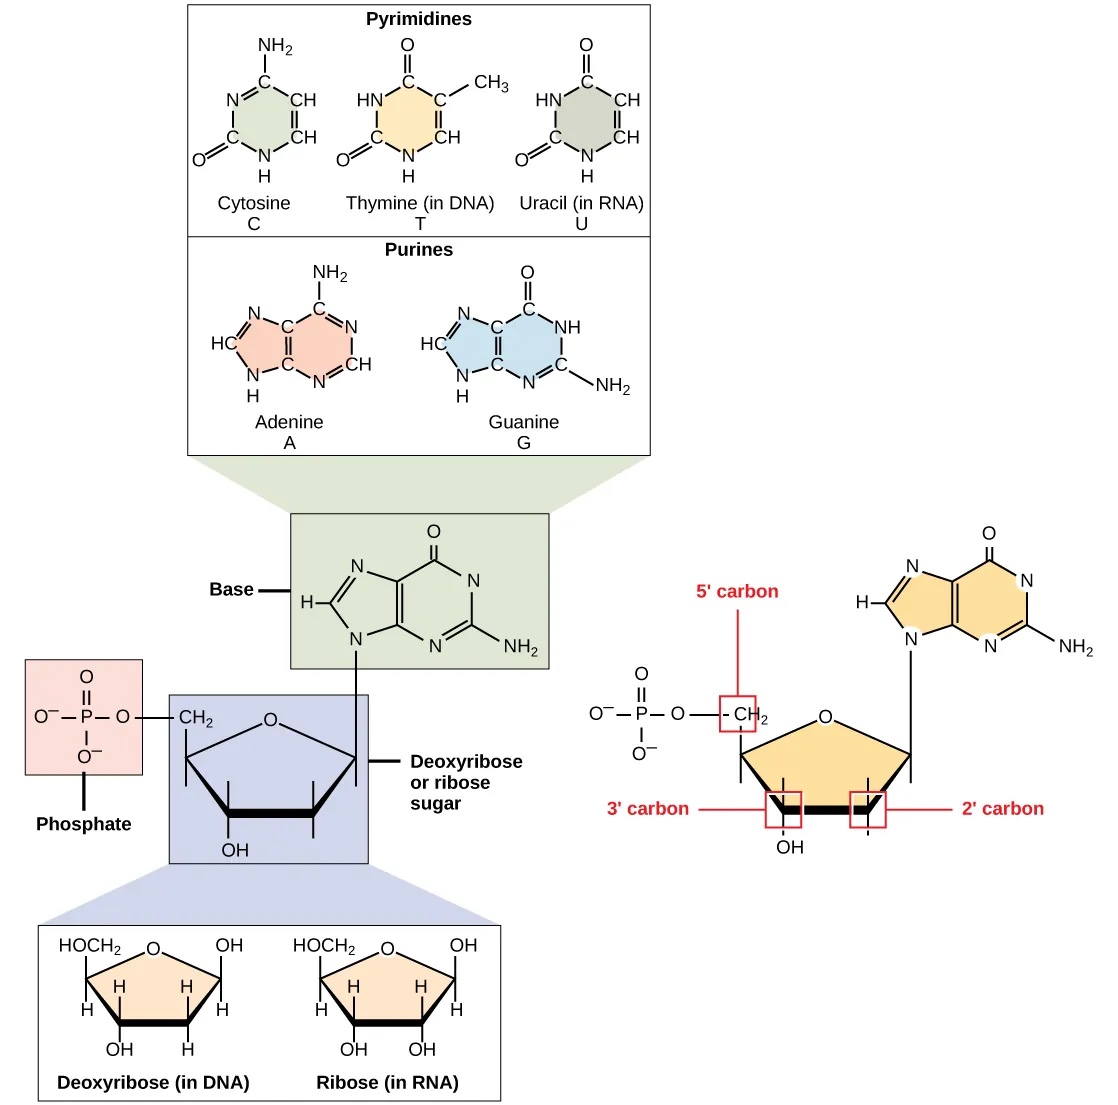
\includegraphics[width=0.9\linewidth]{files/nucleotide-1c35cedc9ecc9b60b760ac4c6644688f.jpg}
\caption[]{The components of a nucleotide.
Credits: \href{https://creativecommons.org/licenses/by/4.0}{CC BY 4.0} \cite{nucleotide_2018}.}
\label{nucleotide}
\end{figure}

The bases can be divided into two categories: purines (with a double ring structure) and pyrimidines (with a single ring structure) (Figure~\ref{nucleotide}).
DNA contains A, T, C, and G; whereas RNA contains A, U, C, and G.

\begin{framed}
\textbf{Important}\\
Nucleotides are central molecules in all life.
You do not need to remember the exact chemical structure, but you need to know the difference between DNA and RNA, the different bases and their category (purines or pyrimidines).
\end{framed}


\bigskip
\centerline{\rule{13cm}{0.4pt}}
\bigskip

\paragraph{The DNA double helix}

The DNA molecule is a polymer of deoxyribonucleotides and forms a right-handed double helix.
The sugar and phosphate are on the outside forming the helix's backbone and the bases are stacked in the interior and bind each other by hydrogen bonds.
Thereby A pairs with T via two hydrogen bonds and C pairs with G via three hydrogen bonds, they are \textbf{complementary} bases.
These pairings are also called Watson-Crick base-pairing, named after the discoverers of DNA.

% :::{figure} images/chapter1/dna.jpg
% :alt: DNA structure
% :width: 70%
% :name: dna
% 
% The DNA structure.
% Credits: {cite}`dna_2008`.
% :::
% #% Unable to use figure dna due to copyright.

\begin{figure}[!htbp]
\centering
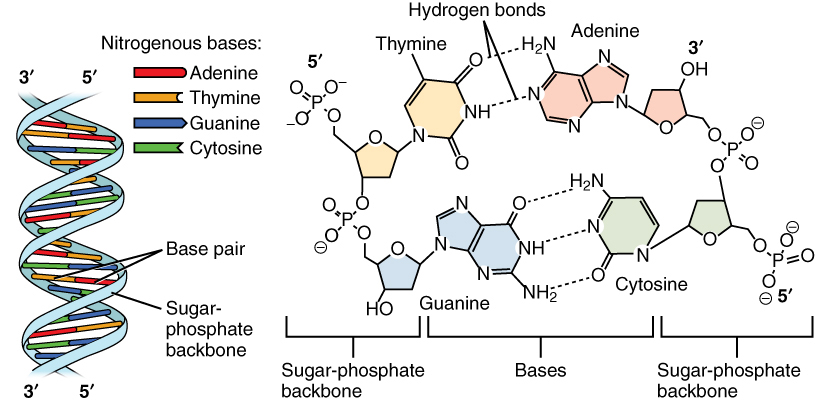
\includegraphics[width=0.8\linewidth]{files/dna_alt-0d35e3218bc7b4f7a3ade1e1f483b3ac.jpg}
\caption[]{The DNA structure.
Credits: \href{https://creativecommons.org/licenses/by/3.0/}{CC BY 3.0} \cite{dna_alt_2013}.}
\label{dna_alt}
\end{figure}

The two strands of the helix run in opposite directions, also called anti-parallel, i.e., one goes from 5' to 3' and the other from 3' to 5' (Figure~\ref{dna_alt}).
The nucleotide sequence is typically written in 5' to 3' direction.
Due to the complementarity, the base sequence of a strand can be deduced from the base sequence from the other strand.
This is called the \textbf{reverse complement}.
For example, the reverse complement of AAGT is ACTT, where both strands are given in 5' to 3' direction.


\bigskip
\centerline{\rule{13cm}{0.4pt}}
\bigskip

\paragraph{DNA replication}\label{chapter1_replication}

As the two DNA strands are only connected via hydrogen bonds, they can be separated relatively easily, for example during DNA replication (Figure~\ref{replication_alt}).
The separated strands each serve as a template on which a new complementary strand is synthesized by the enzyme DNA polymerase in 5' to 3' direction.
This mode of replication is called semiconservative.

% :::{figure} images/chapter1/replication.jpg
% :alt: Replication
% :width: 50%
% :name: replication
% 
% A) The process of DNA replication.
% Credits: [CC0 1.0](https://creativecommons.org/publicdomain/zero/1.0/) {cite}`replication_a_2013`.
% B) Semiconservative DNA replication, where the two copies each contain one original strand and one new strand.
% Credits: [CC BY-SA 2.5](https://creativecommons.org/licenses/by-sa/2.5/) {cite}`replication_b_2005`.
% :::
% #% Unable to use figure replication due to copyright.

\begin{figure}[!htbp]
\centering
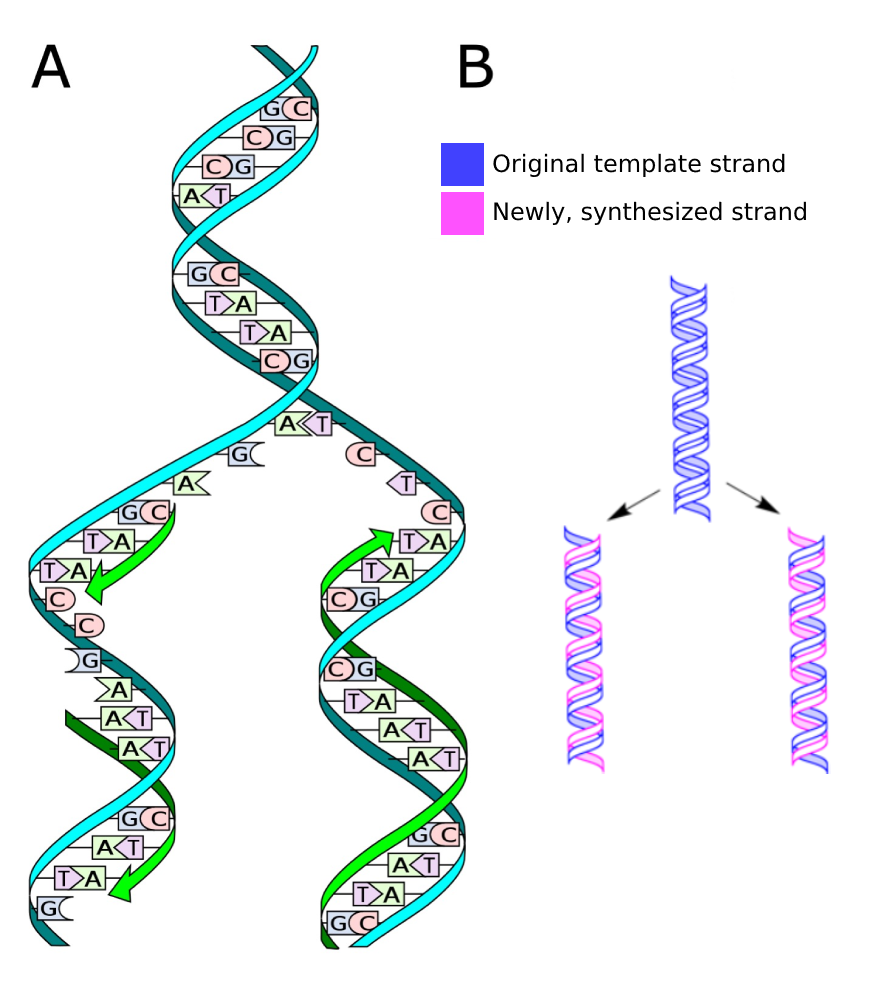
\includegraphics[width=0.5\linewidth]{files/replication_alt-f04199f765869f1200a2c0d77cd5136c.png}
\caption[]{A) The process of DNA replication.
Credits: \href{https://creativecommons.org/publicdomain/zero/1.0/}{CC0 1.0} \cite{replication_a_2013}.
B) Semiconservative DNA replication, where the two copies each contain one original strand and one new strand.
Credits: \href{https://creativecommons.org/publicdomain/zero/1.0/}{CC0 1.0} modified from \cite{replication_b_alt_2009}.}
\label{replication_alt}
\end{figure}

The error rate of DNA replication is remarkably low, about one erroneous base in 10\textsuperscript{9} bases.
This property preserves the genetic information during cell division, and also over generations.
It also leads to mutations over evolutionary time (Figure~\ref{dna_mutation}), as we will see later (Substitutions).

\begin{figure}[!htbp]
\centering
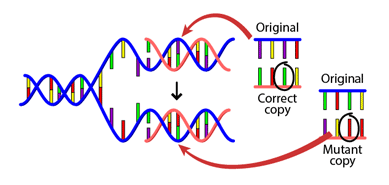
\includegraphics[width=0.5\linewidth]{files/dna_mutation-68a911a7c532b62f50f2909c59238895.png}
\caption[]{A DNA mutation that occurs during replication.
Credits: \href{https://creativecommons.org/licenses/by-nc-sa/4.0/}{BY-NC-SA 4.0} \cite{dna_mutation_2020}.}
\label{dna_mutation}
\end{figure}


\bigskip
\centerline{\rule{13cm}{0.4pt}}
\bigskip

\paragraph{RNA, transcription, and splicing}\label{chapter1_rna_transcription_splicing}

During transcription, RNA polymerase reads the template strand (also called noncoding strand) in the 3' to 5' direction (Figure~\ref{transcription}).
This produces an RNA molecule from 5' to 3', which is a copy of the coding strand.
During transcription thymine is replaced by uracil.
In contrast to DNA, RNA does not form a stable double helix.
RNA is mainly single stranded, but most RNAs show intramolecular base pairing between complementary bases.

There are four major types of RNA:

\begin{itemize}
\item Messenger RNA (mRNA): RNA molecules that will later be translated into proteins and therefore serve as a `messenger' in protein production.
\item Ribosomal RNA (rRNA): the primary component of ribosomes (the `powerplants' of a cell).
\item Transfer RNA (tRNA): functions as `adapter molecule' that serve as the physical link between mRNA and the amino acid sequence of a protein during translation.
\item MicroRNA (miRNA): non-coding RNA molecules of 21-23 nucleotides involved in RNA silencing and post-transcriptional regulation of gene expression.
\end{itemize}

\begin{figure}[!htbp]
\centering
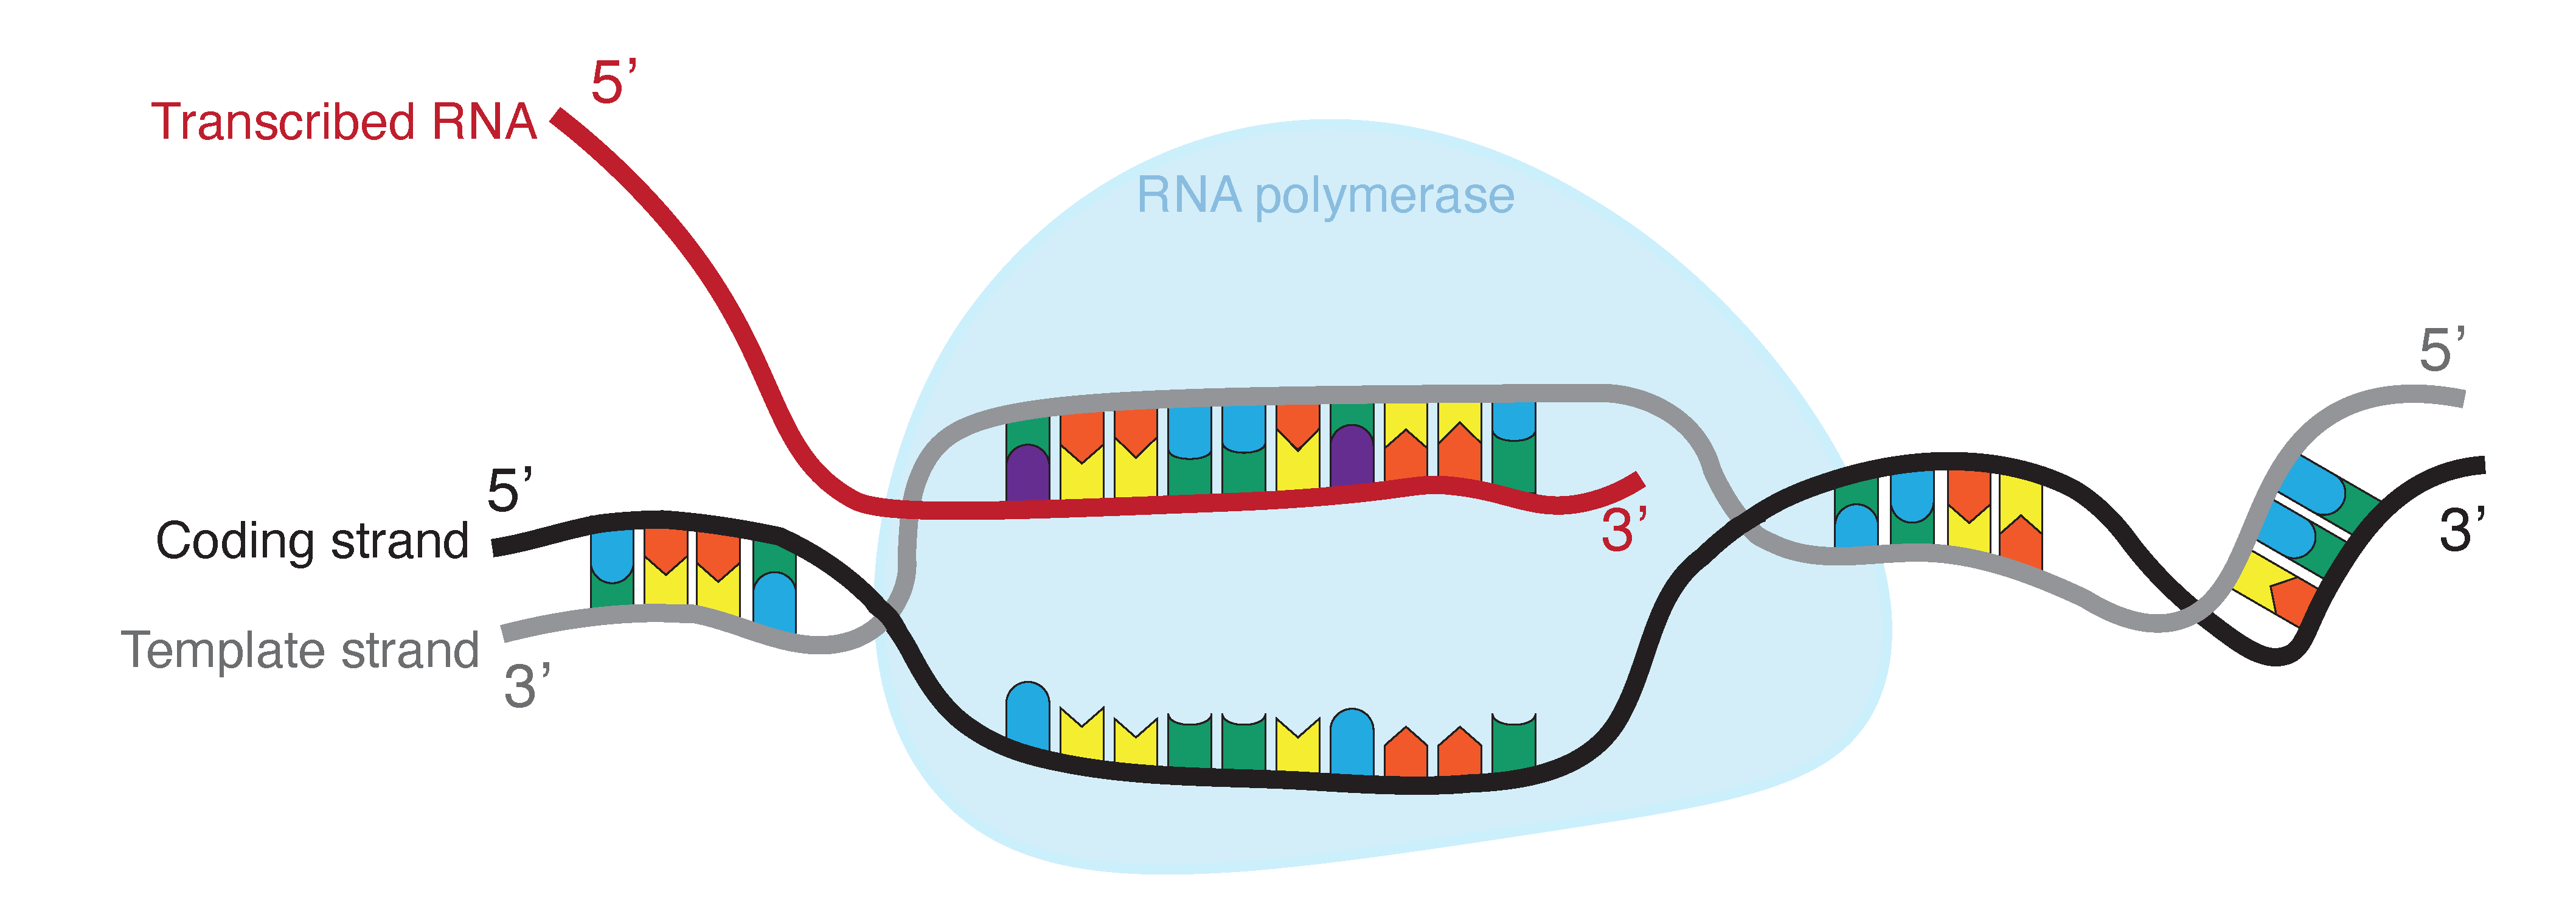
\includegraphics[width=0.7\linewidth]{files/transcription-a75e6e7573d01b067818d6dc4aa4f2fa.png}
\caption[]{RNA is produced by transcribing DNA: as such, it is a direct copy of the information contained in the DNA.
Where DNA contains thymine (T, indicated in blue), RNA contains uracil (U, indicated in purple).
Credits: \href{https://creativecommons.org/licenses/by-nc/4.0/}{CC BY-NC 4.0} \cite{own_1_2024}.}
\label{transcription}
\end{figure}

In eukaryotes, precursor mRNA molecules undergo splicing.
During RNA splicing, the spliceosome protein complex removes introns: specific non-coding parts of an mRNA molecule that are not used during translation (Figure~\ref{splicing}), to create mature mRNA.
Most introns are characterized by a GU and AG dinucleotide motif in the 5' and 3' end respectively.

\begin{figure}[!htbp]
\centering
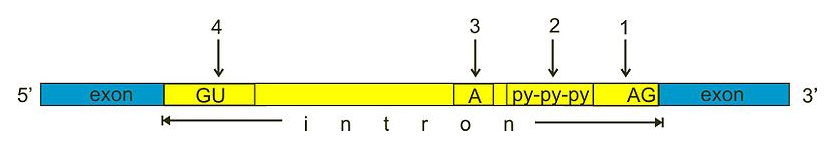
\includegraphics[width=0.7\linewidth]{files/splicing-ae129e41abb4fdbb769ee710d9e66b60.jpg}
\caption[]{During splicing, introns are removed from precursor mRNA moleculus to create mature mRNA.
Most introns contain several canonical elements that help in recognition by the spliceosome and in creating a specific secondary structure of the intronic RNA that facilitates removal: \textbf{(1)} 3' splice site, \textbf{(2)} poly pyrimidine tract, \textbf{(3)} branch site, \textbf{(4)} 5' splice site'.
Credits: \href{https://creativecommons.org/publicdomain/zero/1.0/}{CC0 1.0} \cite{splicing_2011}.}
\label{splicing}
\end{figure}


\bigskip
\centerline{\rule{13cm}{0.4pt}}
\bigskip

\paragraph{Translation}\label{chapter1_translation}

During protein translation, ribosomes synthesize polypeptides from messenger RNA (mRNA) (Figure~\ref{translation_alt}).
During this process tRNAs decode the information on the RNA into amino acids, where a codon consisting of three nucleotides encodes the information for one amino acid.

% :::{figure} images/chapter1/translation.jpg
% :alt: Translation
% :width: 70%
% :name: translation
% 
% The translation process, where ribosomes with tRNA molecules "read" codons on the mRNA using anticodons, which then get translated into their corresponding amino acids.
% These amino acids are linked together by peptide bonds to form a polypeptide chain.
% :::
% #% Unable to use figure translation due to copyright.

\begin{figure}[!htbp]
\centering
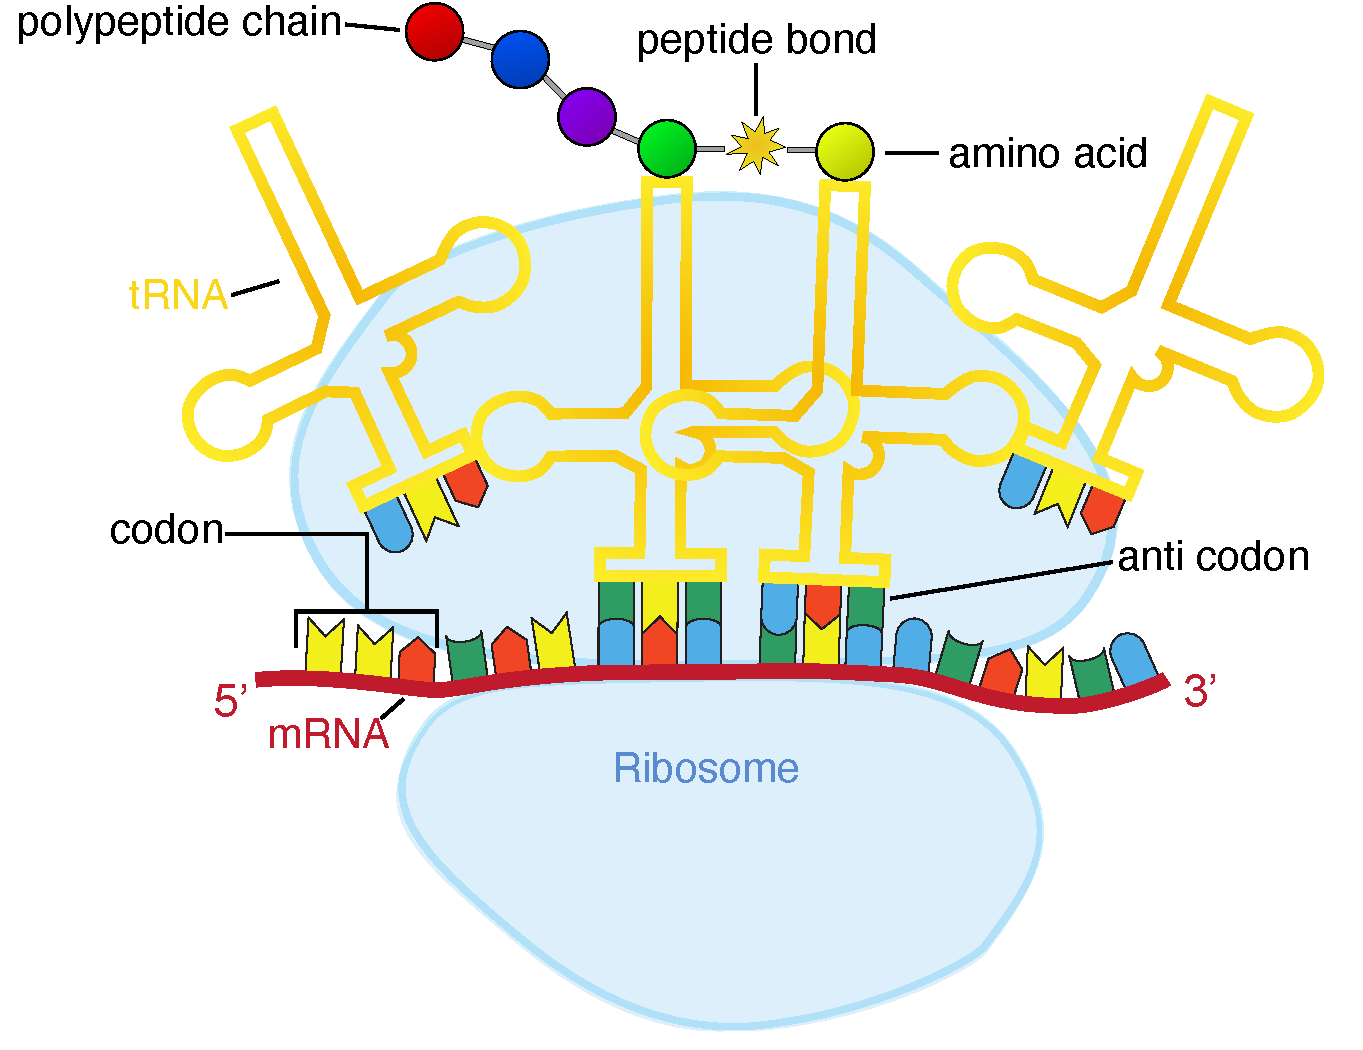
\includegraphics[width=0.7\linewidth]{files/translation_alt-47ee1f3f0d058509ab6b6043187d4a5e.pdf}
\caption[]{The translation process, where ribosomes with tRNA molecules ``read'' codons on the mRNA using anticodons, which then get translated into their corresponding amino acids.
These amino acids are linked together by peptide bonds to form a polypeptide chain.
Credits: \href{https://creativecommons.org/licenses/by-nc/4.0/}{CC BY-NC 4.0} \cite{own_1_2024}.}
\label{translation_alt}
\end{figure}

\begin{framed}
\textbf{See Also}\\
The details of transcription and translation differ between prokaryotes and eukaryotes. You can look up Chapters 15 and 16 of \href{https://openstax.org/details/books/biology-2e}{Biology 2e} to learn more.
\end{framed}

\paragraph{The genetic code}\label{chapter1_genetic_code}

The genetic code shows the correspondence between codons and amino acids (Figure~\ref{geneticcode}).
Since 64 possible codons code for 20 different amino acids, the genetic code is degenerate, i.e., most amino acids are specified by more than one codon.
Thus, the codons encoding one particular amino acid may differ in one or two of their positions.
You can notice in Figure~\ref{geneticcode} that the third codon position often differs between codons for the same amino acid.
As a result of the code degeneracy, the protein sequence can be deduced from the DNA or RNA sequence but not vice versa.

There are three codons that do not encode for an amino acid, but instead signal the end of the protein sequence, called \textbf{stop codons}.
Furthermore, translation generally starts with the start codon AUG encoding methionine.
More information of how protein information is encoded in genomes can be found in the section on genome~annotation.

\begin{figure}[!htbp]
\centering
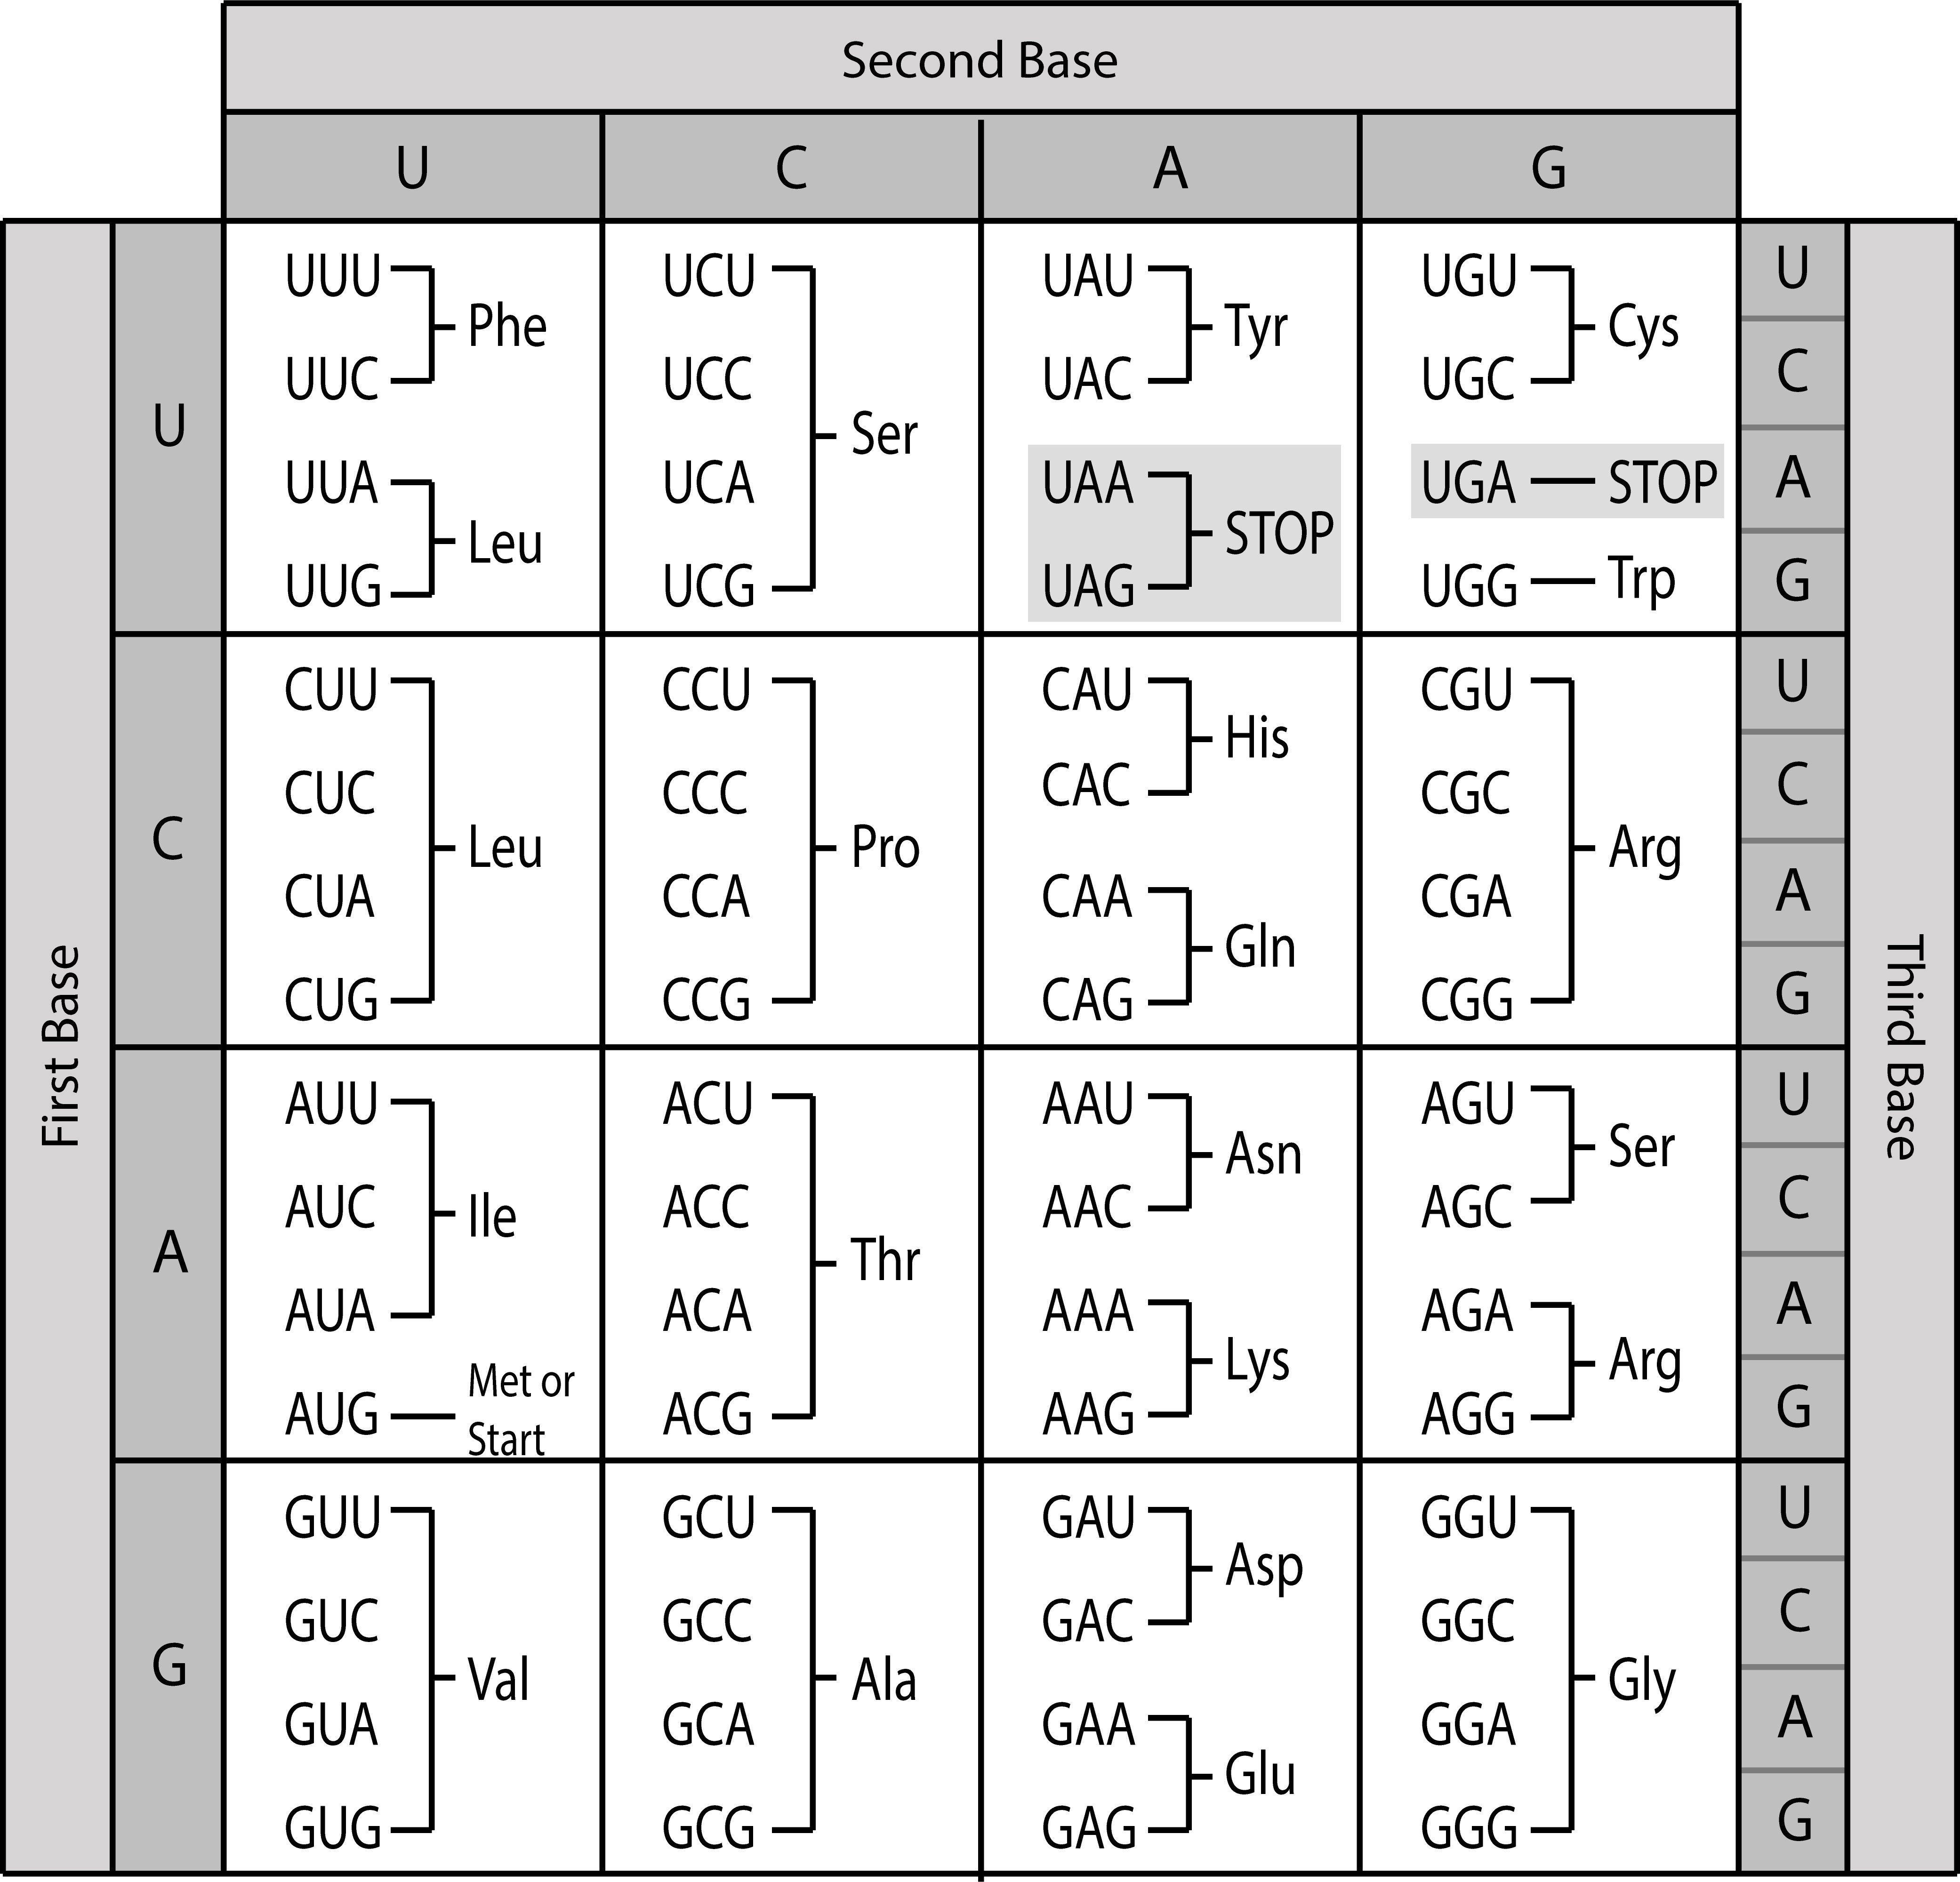
\includegraphics[width=0.8\linewidth]{files/geneticcode-3167edd785c0ef0c20cd7c489c096264.jpg}
\caption[]{The universal genetic code. Note that exceptions to this code exist, for example the vertebrate mitochondrial code.
Credits: \href{https://creativecommons.org/licenses/by/4.0}{CC BY 4.0} \cite{geneticcode_2018}.}
\label{geneticcode}
\end{figure}

\begin{framed}
\textbf{Important}\\
The universal genetic code is very important to understand how information flows from genes to proteins.
Nevertheless, you do not need to recall it, but can always look it up.
When needed, it will also be provided in the exam.
\end{framed}

\paragraph{The central dogma of molecular biology}

According to the central dogma of molecular biology, the flow of genetic information is essentially in one direction: from DNA via RNA to proteins (Figure~\ref{dogma_alt}).
Nevertheless, there are also genes that do not code for proteins, but where functional RNA is the end product. Furthermore, mobile genetic elements and viruses can encode reverse transcriptases (which can synthesize DNA from an RNA template) or RNA dependent RNA polymerases (which can replicate RNA).

% :::{figure} images/chapter1/dogma.jpg
% :alt: Central dogma
% :width: 35%
% :name: dogma
% 
% The central dogma of molecular biology.
% Credits: [CC BY-SA 3.0](https://creativecommons.org/licenses/by-sa/3.0/) {cite}`dogma_2008`.
% :::
% #% Unable to use figure dogma due to copyright.

\begin{figure}[!htbp]
\centering
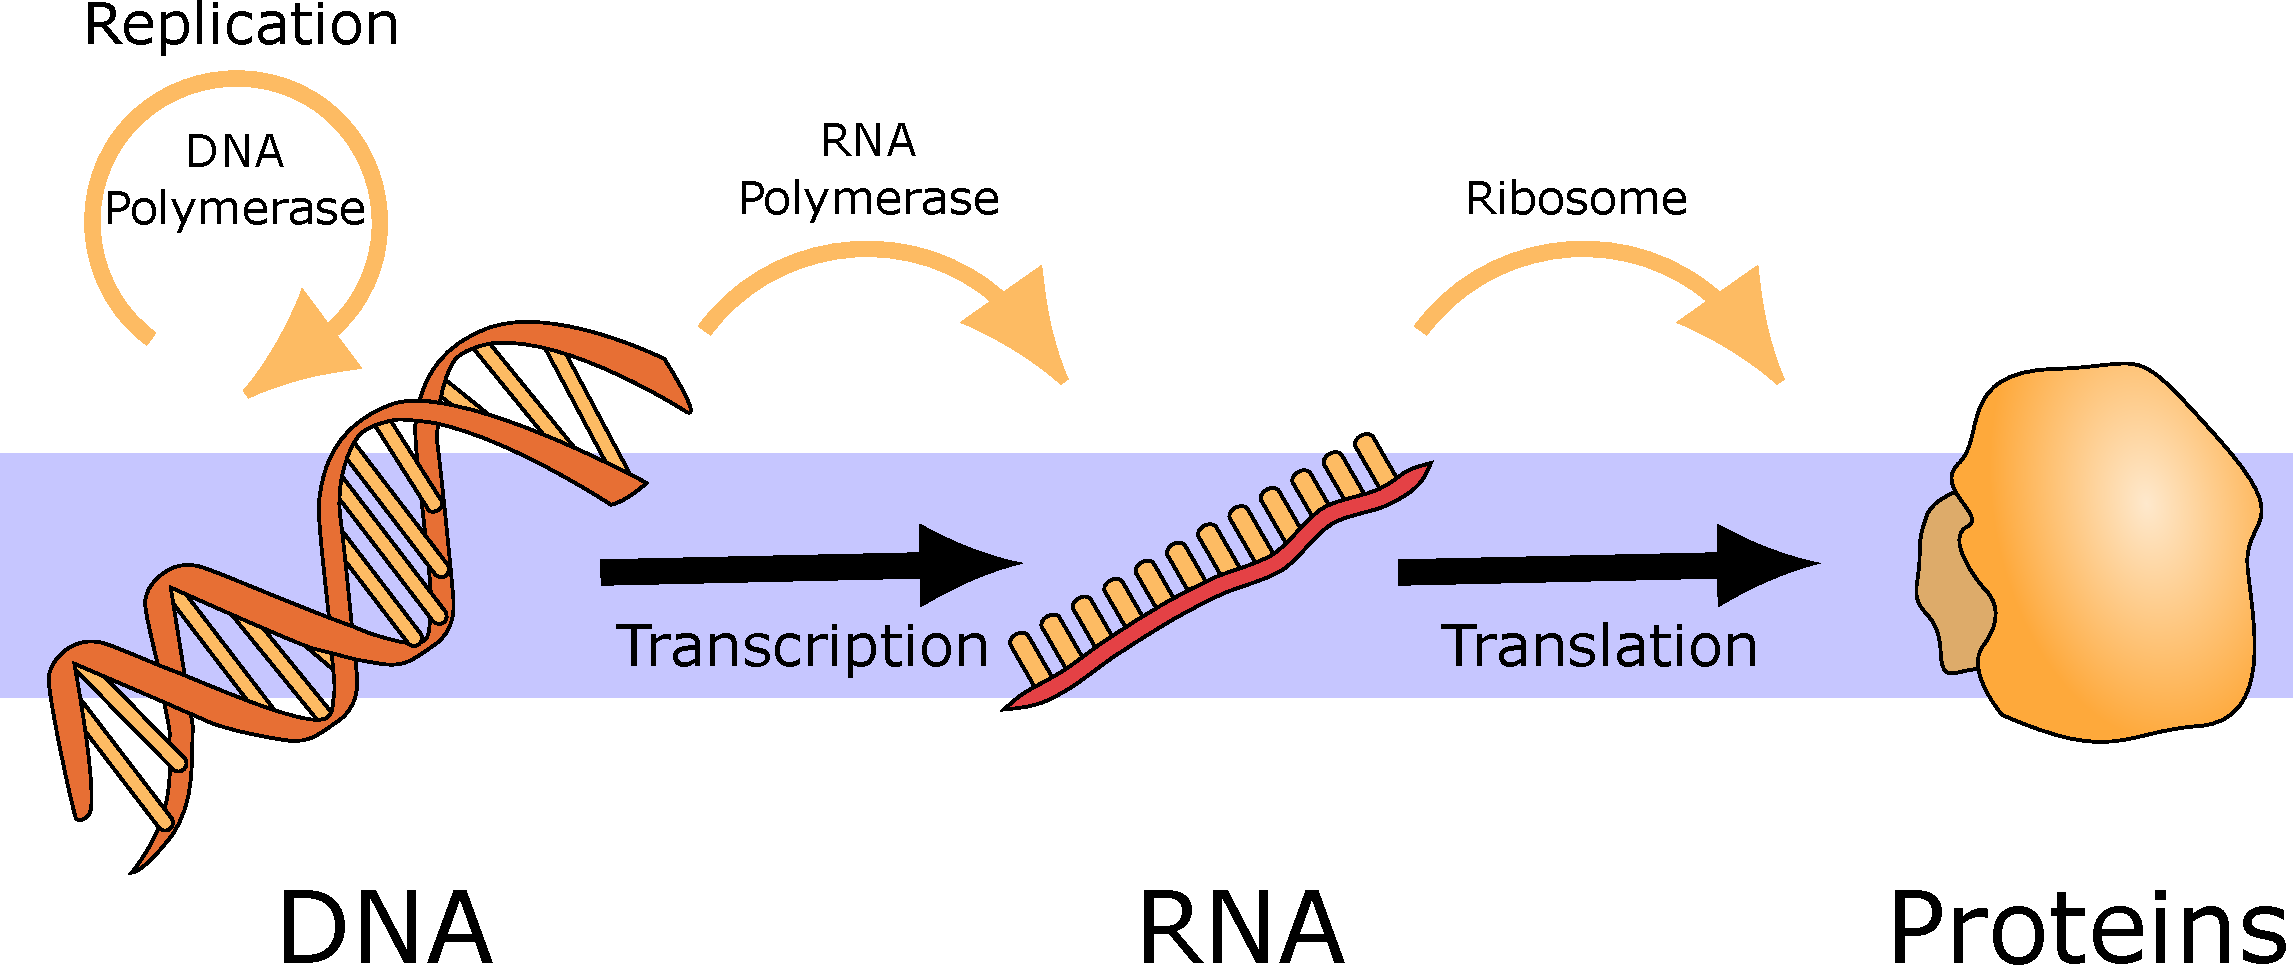
\includegraphics[width=0.8\linewidth]{files/dogma_alt-2d2dc9071cc69db13eb71dff5220b6b2.pdf}
\caption[]{The central dogma of molecular biology.
Credits: \href{https://creativecommons.org/publicdomain/zero/1.0/}{CC0 1.0} modified from \cite{dogma_alt_2008}.}
\label{dogma_alt}
\end{figure}

\paragraph{Proteins}

Proteins are large, complex macromolecules that play many important roles in the body.
They are critical to most of the work done by cells and are required for the structure, function and regulation of the body's tissues and organs.
The basic building blocks of proteins are amino acids.


\bigskip
\centerline{\rule{13cm}{0.4pt}}
\bigskip

\subparagraph{Amino acids}\label{chapter1_aminoacids}

An amino acid contains a central carbon atom (called $\alpha$-carbon, or C\textsubscript{$\alpha$}) (Figure~\ref{aminoacid}).
The $\alpha$-carbon is bound to an amino group (NH\textsubscript{2}), a carboxyl group (COOH), and a hydrogen atom. In addition, each amino acid has a specific residue (R) group.

\begin{figure}[!htbp]
\centering
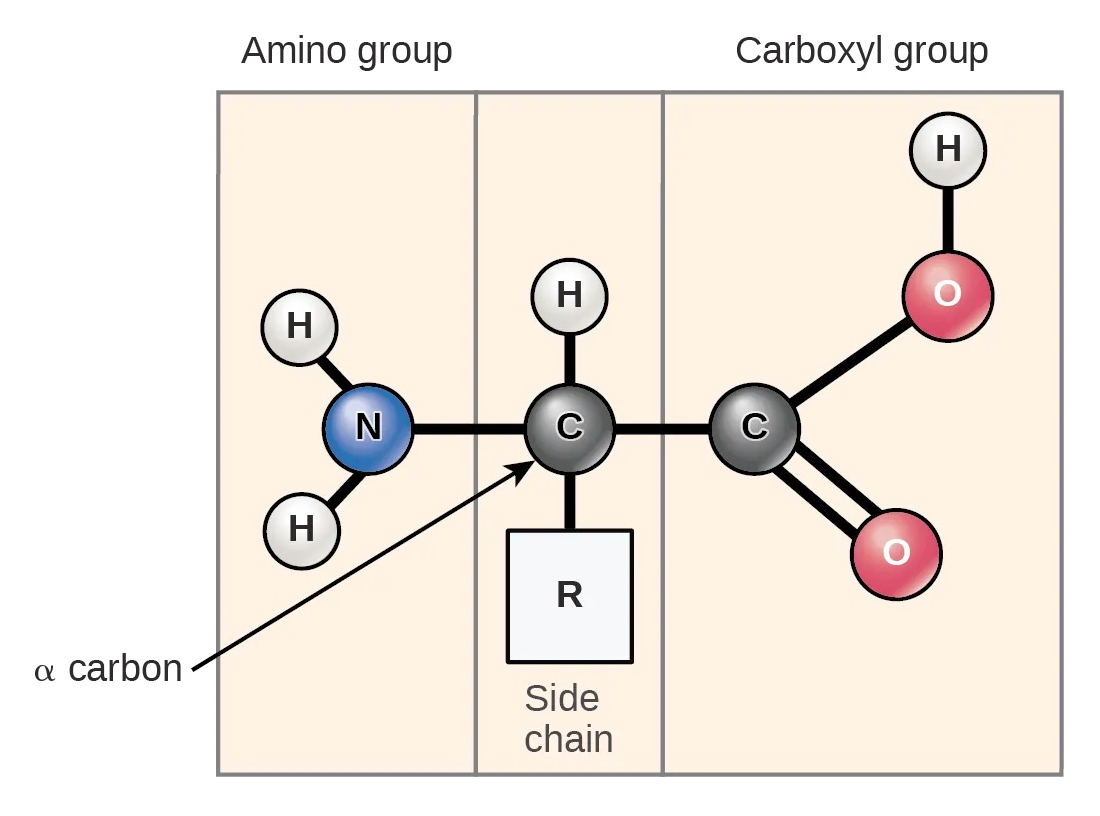
\includegraphics[width=0.6\linewidth]{files/aminoacid-43fb3a83f9ded9cb29064fb29d80b29c.jpg}
\caption[]{The structure of an amino acid.
Four elements are connected to the $\alpha$-carbon: an amino group, a hydrogen atom, a carboxyl group, and a side chain (R group).
Credits: \href{https://creativecommons.org/licenses/by/4.0}{CC BY 4.0} \cite{proteins_2018}.}
\label{aminoacid}
\end{figure}

\begin{framed}
\textbf{Important}\\
Amino acids differ in their chemical properties, which are determined by their R groups.
It is important to know (by heart) the amino acids, their one-letter and three-letter abbreviation, and their fundamental properties as given in the table.
\end{framed}

\begin{table}
\centering
\caption[]{Amino acids and their abbreviations and basic properties}
\label{aminoacidtable}
\begin{tabular}{p{\dimexpr 0.250\linewidth-2\tabcolsep}p{\dimexpr 0.250\linewidth-2\tabcolsep}p{\dimexpr 0.250\linewidth-2\tabcolsep}p{\dimexpr 0.250\linewidth-2\tabcolsep}}
\toprule
Amino acid & Three-letter code & One-letter code & Property \\
\hline
Arginine & Arg & R & Positively charged \\
Histidine & His & H & Positively charged \\
Lysine & Lys & K & Positively charged \\
Aspartic acid & Asp & D & Negatively charged \\
Glutamic acid & Glu & E & Negatively charged \\
Serine & Ser & S & Polar uncharged \\
Threonine & Thr & T & Polar uncharged \\
Asparagine & Asn & N & Polar uncharged \\
Glutamine & Gln & Q & Polar uncharged \\
Alanine & Ala & A & Hydrophobic \\
Valine & Val & V & Hydrophobic \\
Isoleucine & Ile & I & Hydrophobic \\
Leucine & Leu & L & Hydrophobic \\
Methionine & Met & M & Hydrophobic \\
Phenylalanine & Phe & F & Hydrophobic and aromatic \\
Tyrosine & Tyr & Y & Hydrophobic and aromatic \\
Trypotophan & Trp & W & Hydrophobic and aromatic \\
Glycine & Gly & G & Special (only H as side chain) \\
Proline & Pro & P & Special (side chain bound to backbone nitrogen) \\
Cysteine & Cys & C & Special (forms disulfide bonds) \\
\bottomrule
\end{tabular}
\end{table}

Some amino acids have non-polar side chains, and these are generally \textbf{hydrophobic}, i.e., water molecules cannot form hydrogen bonds with these molecules.
Thus, they can often be found in the interior of proteins together with other hydrophobic amino acids.
\textbf{Aromatic} amino acids contain aromatic rings, and often stabilize folded protein structures.

In contrast, the charged and the polar amino acids are \textbf{hydrophilic}, i.e., water molecules can form hydrogen bonds with these molecules.
They can often be found on the surface of proteins or in the interior, when they can interact with another oppositely charged amino acid.
\textbf{Positively charged} amino acids, are also called basic amino acids and \textbf{negatively charged} amino acids are also called acidic amino acids.

Although amino acids can be classified into these groups based on their properties, some amino acids stand out.
The smallest amino acid is glycine, which provides great flexibility due to its small size.
In contrast, proline is an amino acid, where the side chain is bonded to the backbone nitrogen atom, which makes it very rigid.


\bigskip
\centerline{\rule{13cm}{0.4pt}}
\bigskip

\subparagraph{Protein structure}\label{chapter1_protein_structure}

A protein is made up of one or more long, folded chains of amino acids (each called a \textbf{polypeptide}).
The 3D structure of a protein is also called its \textbf{conformation}.
The protein conformation is described on four levels - primary to quaternary structure (Figure~\ref{struclevels_alt}).

% :::{figure} images/chapter1/struclevels.jpg
% :alt: The four levels of protein structure
% :width: 90%
% :name: struclevels
% 
% The four levels of protein structure.
% Credits: Rao, A. Ryan, K. and Tag, A. Department of Biology, Texas A&M University.
% :::
% #% Unable to use figure struclevels due to copyright.

\begin{figure}[!htbp]
\centering
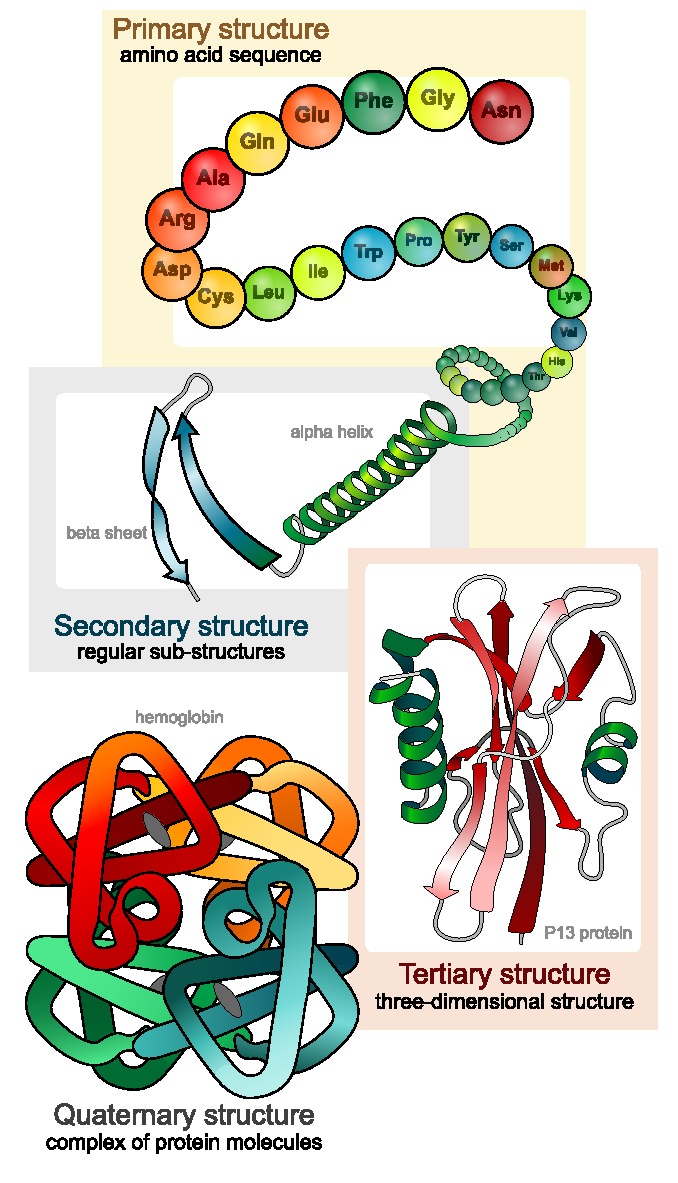
\includegraphics[width=0.6\linewidth]{files/struclevels_alt-0651e6addf2ddae34e55d1fbb7a283cd.pdf}
\caption[]{The four levels of protein structure.
Credits: \href{https://creativecommons.org/publicdomain/zero/1.0/}{CC0 1.0} \cite{struclevels_alt_2008}.}
\label{struclevels_alt}
\end{figure}

The structure of a protein is critical for its function.
For example, in an enzyme, the active site must be in the correct structure to be able to bind the substrate.
Other proteins might bind proteins (and influence their activity) or bind DNA (and regulate gene expression).
Additionally, some proteins are secreted from the cell or might function within the cell membrane.
Finally, proteins are often modified after protein synthesis (see Translation), called post-translational modification.
These modifications can be important for protein function.


\bigskip
\centerline{\rule{13cm}{0.4pt}}
\bigskip

\subparagraph{Primary structure}

In a protein, amino acids are connected by covalent bonds, called peptide bonds.
A peptide bond connects one amino acid's carobxyl group and the next amino acid's amino group (Figure~\ref{peptidebond}).
The sequence of amino acids linked by peptide bonds is called the \textbf{primary structure}.
The protein sequence is determined by the gene sequence encoding the protein.
The continuous chain of atoms along the protein is also called the \textbf{backbone}, it consists of the three backbone atoms (nitrogen, C\textsubscript{$\alpha$}, carbon).

\begin{figure}[!htbp]
\centering
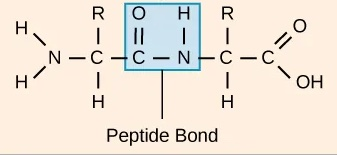
\includegraphics[width=0.4\linewidth]{files/peptidebond-e8f0cd028cafbd2c5d54433c3d2dae1a.jpg}
\caption[]{A peptide bond connecting two amino acids.
Credits: \href{https://creativecommons.org/licenses/by/4.0}{CC BY 4.0} \cite{proteins_2018}.}
\label{peptidebond}
\end{figure}

Each protein has a free amino group on one end, called the \textbf{N terminus}.
The other end has a free carboxyl group, called the \textbf{C terminus}.

\begin{framed}
\textbf{Note 1.1: possible polypeptide chains}\\
As there are 20 distinct amino acids, there can be a huge number of different polypeptide chains, i.e., 20\textsuperscript{n} for a polypeptide of length n.
Most of these potential sequences do not adopt a stable conformation, thus only a tiny fraction of these possibilities exist in nature.
\end{framed}


\bigskip
\centerline{\rule{13cm}{0.4pt}}
\bigskip

\subparagraph{Secondary structure}\label{chapter1_secondary_structure}

Secondary structures are local conformations in the protein that are stabilized by hydrogen bonds between backbone atoms.
We distinguish the regular helices (i.e., alpha helix - $\alpha$-helix) and sheet structures (i.e., beta sheet - $\beta$-sheet) (Figure~\ref{secstructure_alt}) and irregular turns.

\textbf{$\alpha$-helices} are stabilized by hydrogen bonds between the oxygen atom in the C group in one amino acid, and the hydrogen in the N group of the amino acids that is four amino acids farther along the chain.
Every helical turn has 3.6 amino acids residues and the side chains stick out of the helix.

$\beta$-pleated sheets (short: \textbf{$\beta$-sheets}) consist of $\beta$-strands, where the R groups extend above and below the strands.
The strands have a direction determined by the N- and C-terminus of the protein and are usually depicted as an arrow pointing towards the C-terminus.
Depending on the direction, strands can align parallel or antiparallel to each other.

% :::{figure} images/chapter1/secstructure.jpg
% :alt: Secondary structure elements
% :width: 80%
% :name: secstructure
% 
% α-helices and β-sheets are stablized by hydrogen bonds between the backbone of proteins, i.e., the side chains are not involved.
% The hydrogen bonds form between the oxygen atom in the C group in one amino acid and the hydrogen in the N group.
% Black = carbon, white = hydrogen, blue = nitrogen, and red = oxygen. Credits: Rao, A., Tag, A. Ryan, K. and Fletcher, S. Department of Biology, Texas A&M University.
% :::
% #% Unable to use figure secstructure due to copyright.

\begin{figure}[!htbp]
\centering
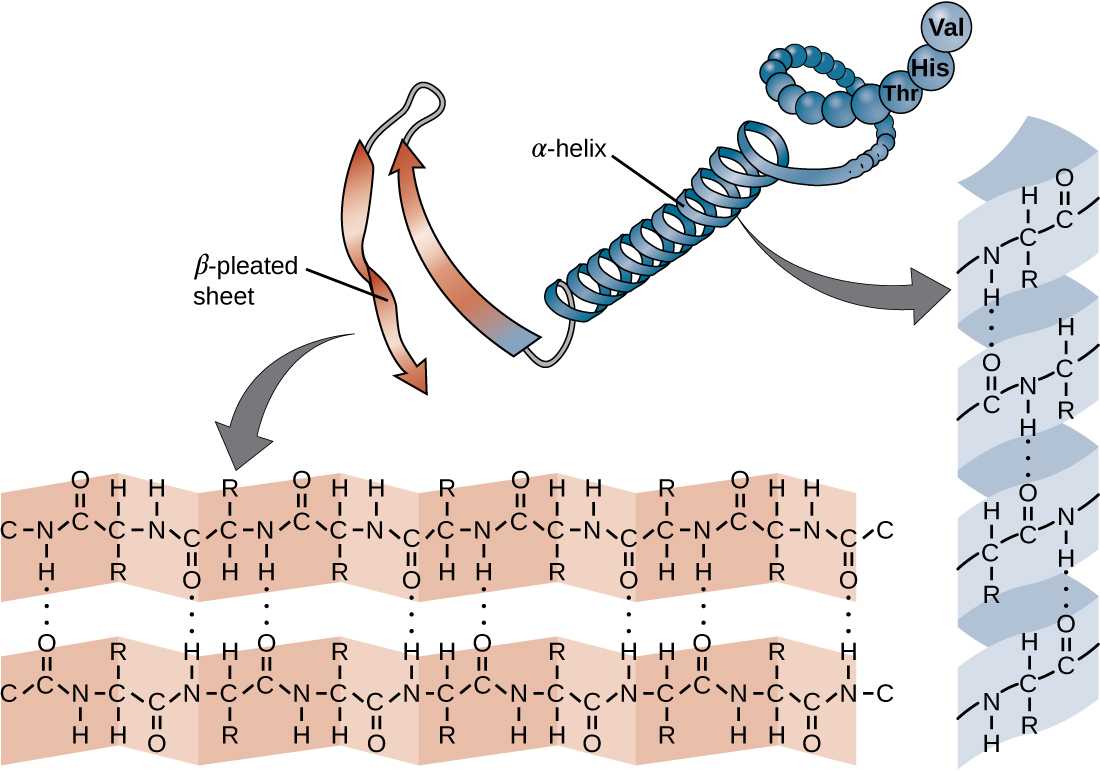
\includegraphics[width=0.8\linewidth]{files/secstructure_alt-aad81a4d80b9af3bc2a1f645520d36e5.jpg}
\caption[]{$\alpha$-helices and $\beta$-sheets are stablized by hydrogen bonds (the dotted lines) between the backbone of proteins, i.e., the side chains are not involved.
The hydrogen bonds form between the oxygen atom in the C group in one amino acid and the hydrogen in the N group.
Credits: \href{https://creativecommons.org/licenses/by/4.0}{CC BY 4.0} modified from \cite{secstructure_alt_nd}.}
\label{secstructure_alt}
\end{figure}

\textbf{Turns} are short secondary structure elements that are stabilized by hydrogen bonds between amino acids that are 1 to 5 peptide bonds away.
The most common form are $\beta$-turns, which connect antiparallel $\beta$-strands.

\begin{framed}
\textbf{Note 1.2: Secondary structure amino acid preference}\\
Although secondary structure elements are formed by hydrogen bonds between the backbone, certain amino acids are favoured in secondary structures and others are disfavoured.
For example, methionine, alanine, leucine, and glutamic acid are favoured in $\alpha$-helices, whereas proline, glycine, and tyrosine are disfavoured.
Also, valine, isoleucine, tyrosine, cysteine, tryptophan, phenylalanine, and threonine are more frequently found in $\beta$-sheets, compared to $\alpha$-helices.
In turns, glycine, asparagine, proline, and serine are preferred.
These preferences are used to predict secondary structure elements in proteins (see chapter~4).
\end{framed}

The peptide bond is very rigid and planar, i.e., it cannot rotate to form the elements of protein structure.
However, the N-C\textsubscript{$\alpha$} and the C\textsubscript{$\alpha$}-C bonds can freely rotate, being only limited by the size and properties of the R-groups.
The 3D shape of the polypeptide backbone is thus determined by two \textbf{torsion angles}:
phi ($\varphi$) between N and C\textsubscript{$\alpha$} and psi ($\psi$) between C\textsubscript{$\alpha$} and C (Figure~\ref{phipsi_alt}A).
Although $\varphi$ and $\psi$ can rotate in principle, steric hindrance prevents certain combinations of angles, i.e., the bulkiness of the R-groups restricts the possible conformations.
Thus, certain combinations of $\varphi$ and $\psi$ are preferred.
We can plot the combinations of $\varphi$ and $\psi$ in a protein, in a so-called \textbf{Ramachandran plot} (Figure~\ref{phipsi_alt}B).

The regular secondary structure elements ($\alpha$-helix and $\beta$-sheet) contain consecutive amino acids with similar ($\varphi$,$\psi$) values.
These regions are typically highly populated in a Ramachandran plot.
Thus, the Ramachandran plot can be used to assess how plausible a predicted protein structure is.

% :::{figure} images/chapter1/phipsi.jpg
% :alt: Phi, psi, and Ramachandran plot
% :width: 70%
% :name: phipsi
% 
% A) Peptide bond, φ, and ψ.
% B) A typical Ramachandran plot. The regions marked "core" do not have any steric hindrance.
% Yellow areas are generally allowed.
% White areas represent conformations that are generally sterically unfavorable.
% Credits: {cite}`phipsi_2014`.
% :::
% #% Unable to use figure phipsi due to copyright.

\begin{figure}[!htbp]
\centering
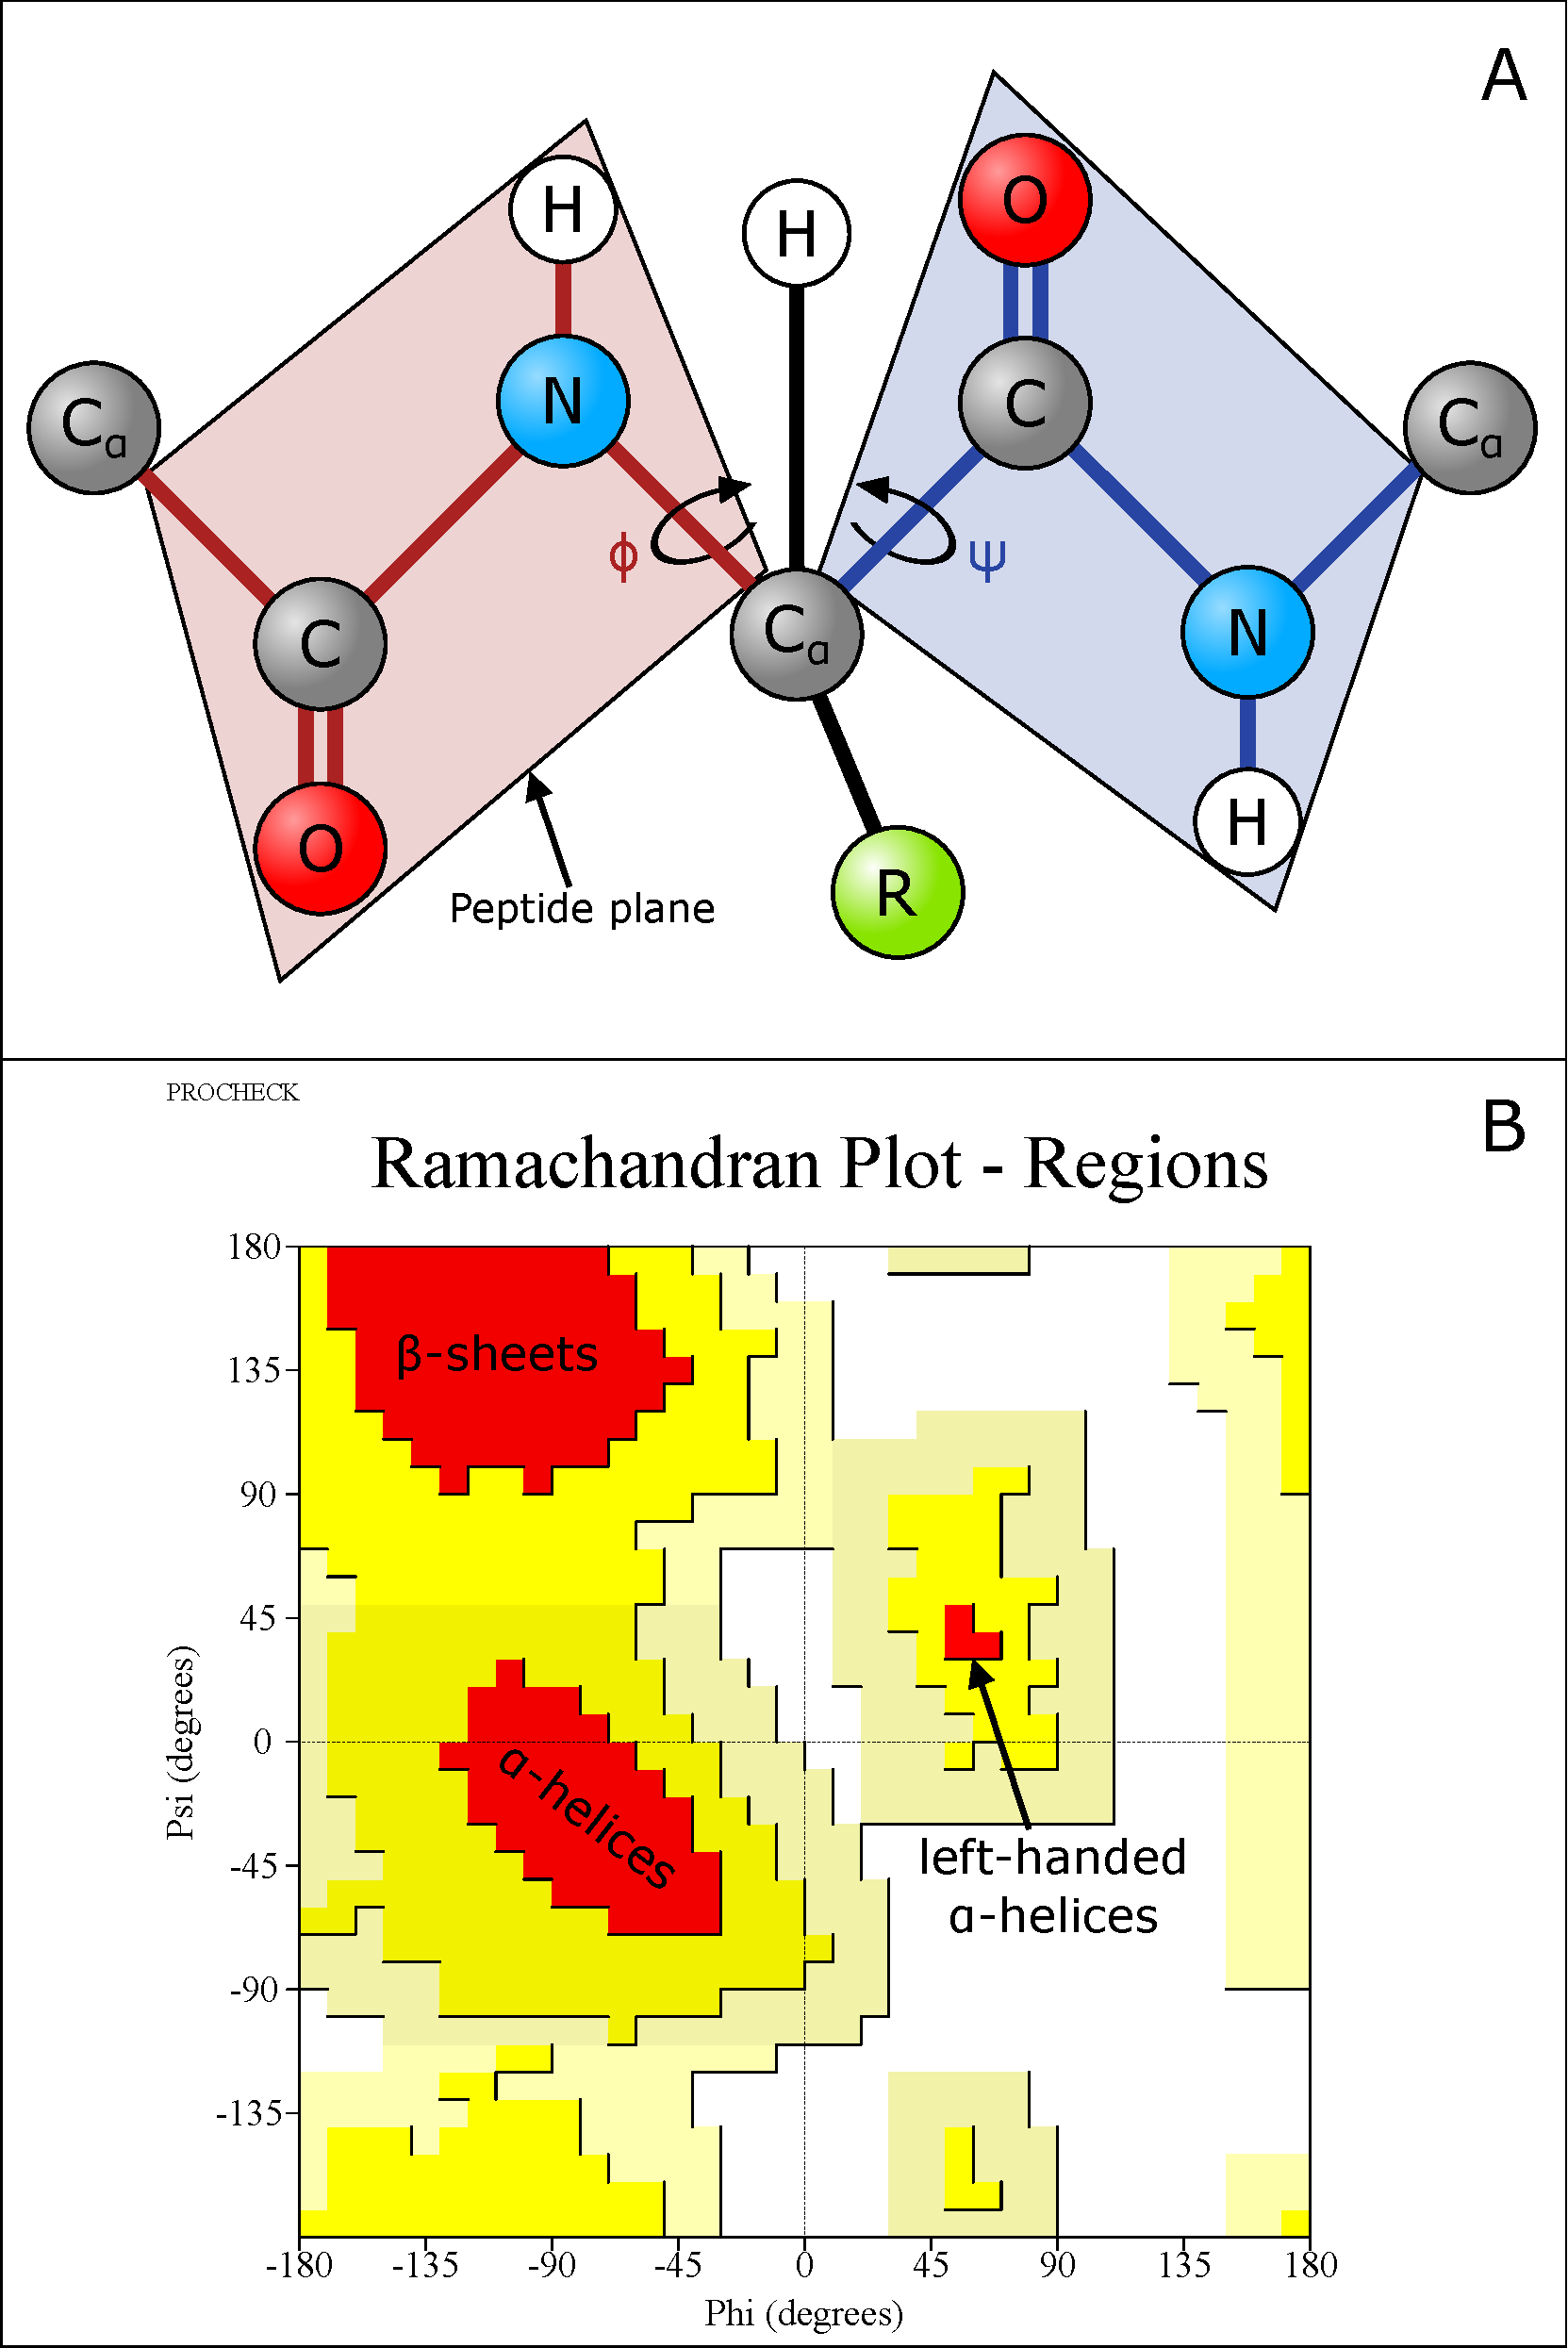
\includegraphics[width=0.5\linewidth]{files/phipsi_alt-4119b9376f7dfe565d87043a7e7a0417.pdf}
\caption[]{A) The $\varphi$, and $\psi$ torsion angles of a polypeptide chain. Credits: \href{https://creativecommons.org/licenses/by-nc/4.0/}{CC BY-NC 4.0} \cite{own_1_2024}.
B) A typical Ramachandran plot. The red regions marked do not have any steric hindrance, yellow areas represent conformations that have steric hindrance, light yellow areas represent conformations that are generally sterically unfavorable, and white areas do not have any allowed conformations.
Credits: Ramachandran plot modified from \href{https://www.ebi.ac.uk/thornton-srv/software/PROCHECK/index.html}{PROCHECK} \cite{procheck_1993}.}
\label{phipsi_alt}
\end{figure}

\begin{framed}
\textbf{See Also}\\
An illustrative animation on $\varphi$ and $\psi$.
\end{framed}


\bigskip
\centerline{\rule{13cm}{0.4pt}}
\bigskip

\subparagraph{Tertiary structure}

The tertiary structure of a protein describes the complete folding of an entire polypeptide chain.
In contrast to the secondary structure, the tertiary structure of a protein involves interactions between the amino acid's side chains that can occur at short-range and long-range (Figure~\ref{terstructure}).
Thus, the chemical properties of the amino acids are very important for the tertiary structure.
Different types of interactions stabilize the tertiary structure:

\begin{itemize}
\item Hydrogen bonds involving polar amino acids.
\item Ionic bonds between positively and negatively charged amino acids.
\item Hydrophobic R groups that tend to lie in the protein's interior, stabilized by hydrophobic interactions.
\item Disulfide bonds (i.e., covalent bonds between cysteines).
\end{itemize}

\begin{figure}[!htbp]
\centering
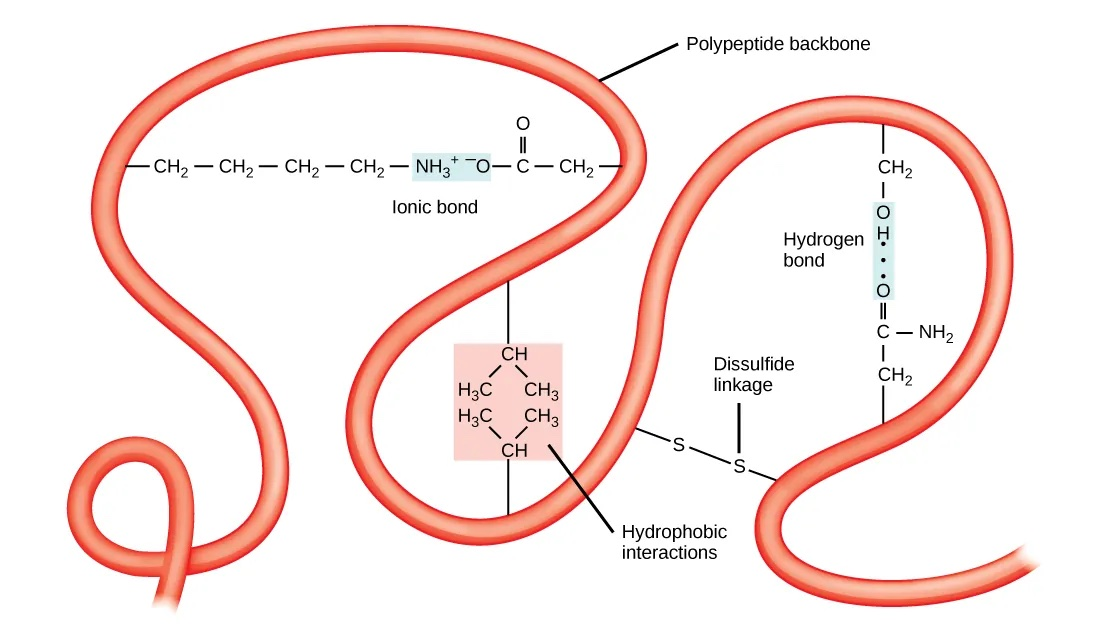
\includegraphics[width=0.8\linewidth]{files/terstructure-4b7f78306caf16f9c7283bc23fe4a55b.jpg}
\caption[]{Chemical interactions that stabilize the tertiary structure of proteins.
Credits: \href{https://creativecommons.org/licenses/by/4.0}{CC BY 4.0} \cite{proteins_2018}.}
\label{terstructure}
\end{figure}

\begin{framed}
\textbf{Note 1.3: Denaturation}\\
The noncovalent bonds that stabilize the protein structure are broken at high temperature.
Thus, most proteins unfold above about 60°C.
This process is called denaturation and is generally irreversible.
When proteins denature, they lose their function.
\end{framed}

\textbf{Domains} are distinct functional and/or structural units in a protein and are typically 50 to 350 amino acids long.
Usually, a domain is responsible for a particular function or interaction, contributing to the overall role of a protein.
A domain can exist in different contexts with other domains (Figure~\ref{domains}).
In a multidomain protein, each domain folds independently of the others.

\begin{figure}[!htbp]
\centering
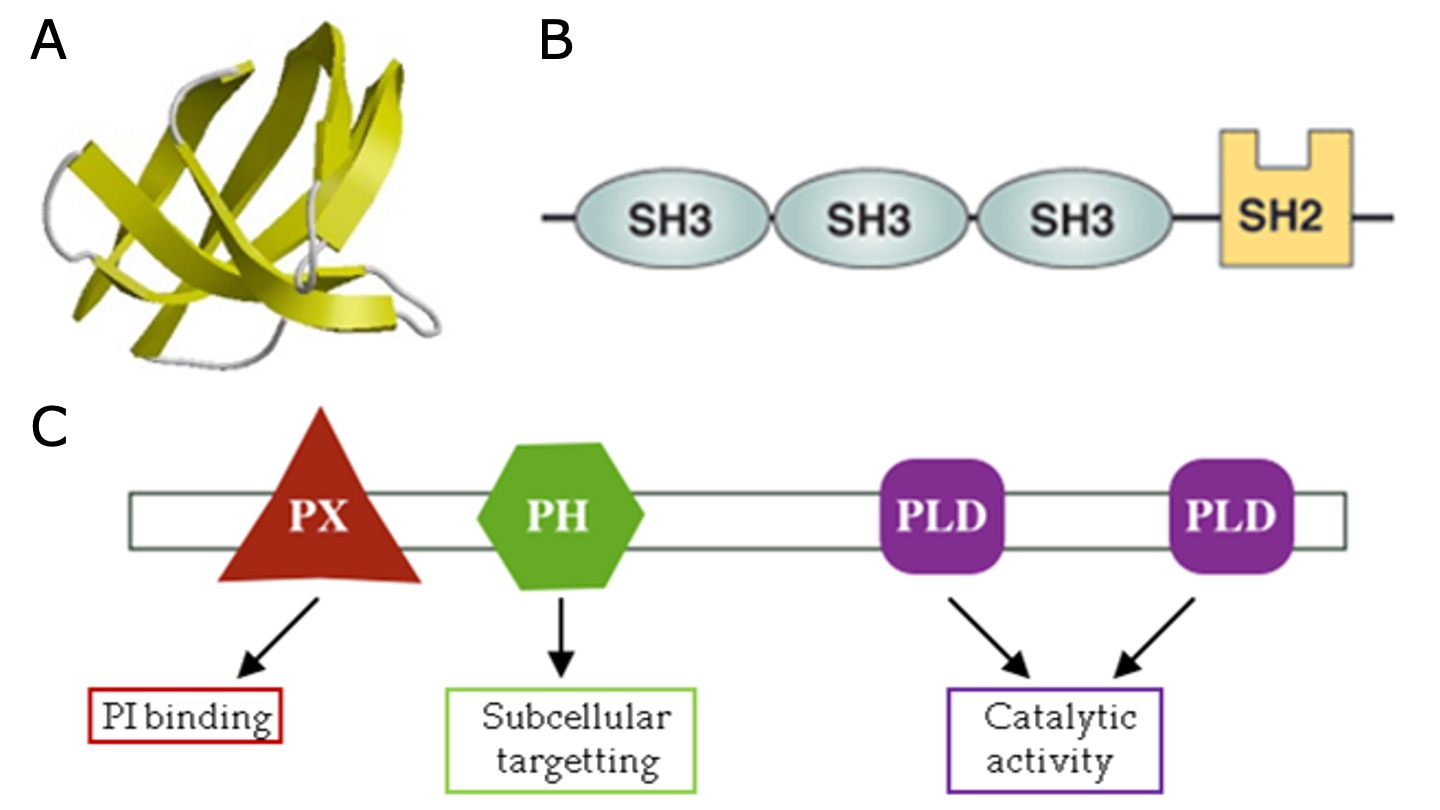
\includegraphics[width=0.7\linewidth]{files/domains-7cca8056e5affaf9aa34f387f50bc335.jpg}
\caption[]{A) Example of an Src homology 3 (SH3) domain that is involved in protein-protein interaction. SH3 domains occur in a diverse range of proteins with different functions.
B) The cytoplasmic protein Nck contains multiple SH3 domains.
C) Domain composition of phospholipase D1, which has multiple functional domains that contribute to its overall function.
Credits: \href{https://creativecommons.org/licenses/by/4.0}{CC BY 4.0} \cite{domains_2023}.}
\label{domains}
\end{figure}


\bigskip
\centerline{\rule{13cm}{0.4pt}}
\bigskip

\subparagraph{Quaternary structure}

Finally, individual folded polypeptides can interact to form \textbf{protein complexes}, also called quaternary structures.
The quaternary structure is stabilized by the same types of interactions as the tertiary structure.
The difference is that the amino acids involved belong to different polypeptides.

Many functional proteins are composed of multiple subunits, they are also called \textbf{oligomers} (Figure~\ref{oligomers}).
The subunits can originate from the same protein sequence (called a homomer) or from different sequences (called a heteromer).
Proteins consisting of two subunits are also called dimer.

\begin{figure}[!htbp]
\centering
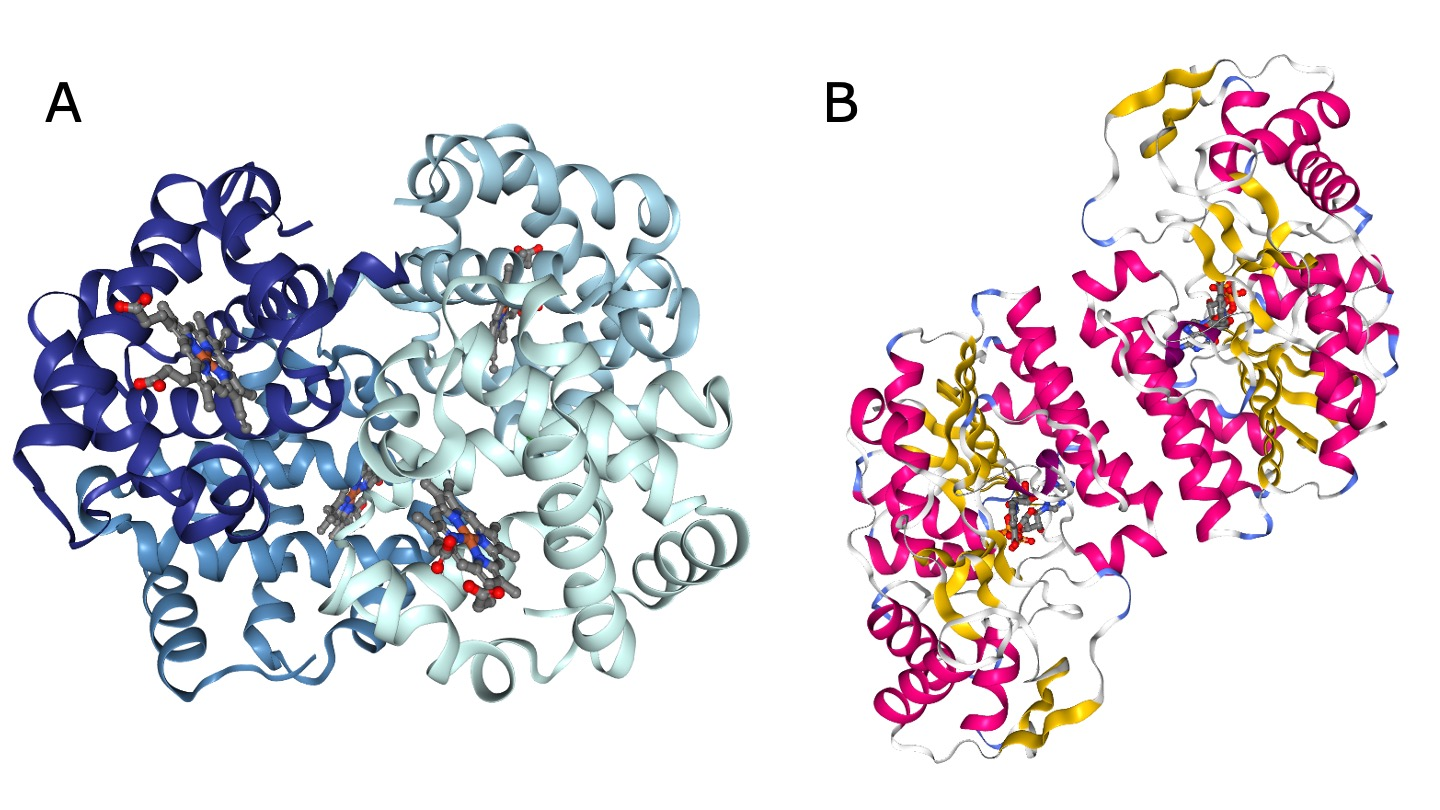
\includegraphics[width=0.7\linewidth]{files/oligomers-eac46cb02a81a2c53b32d003ffc2198f.jpg}
\caption[]{Examples of oligomers.
A) Myoglobin, a heteromer of four subunits (PDB structure 1HV4 colored by chain). Credits: \citet{rcsb_2000, oligomers_a_2001, ngl_2018}.
B) UDP-galactose 4-epimerase, a homodimer (PDB structure 1EK5 colored by secondary structure). Credits: \citet{rcsb_2000, oligomers_b_2000, ngl_2018}.}
\label{oligomers}
\end{figure}


\bigskip
\centerline{\rule{13cm}{0.4pt}}
\bigskip

\subparagraph{Substitutions}\label{chapter1_substitutions}

Mutations in the gene sequence can lead to changes in the primary structure of the protein, e.g., a substitution of one amino acid by a different one.
Often, such substitutions still lead to highly similar protein structures that perform a similar or even the same function, especially when the exchanged amino acids have similar chemical properties.
Nevertheless, single amino acid substitutions can have severe consequences.
A prominent example is sickle cell anemia, where a substitution of valine to glutamic acid in hemoglobin $\beta$ results in a structural change that leads to a distortion in red blood cells (Figure~\ref{sicklecell}).

\begin{figure}[!htbp]
\centering
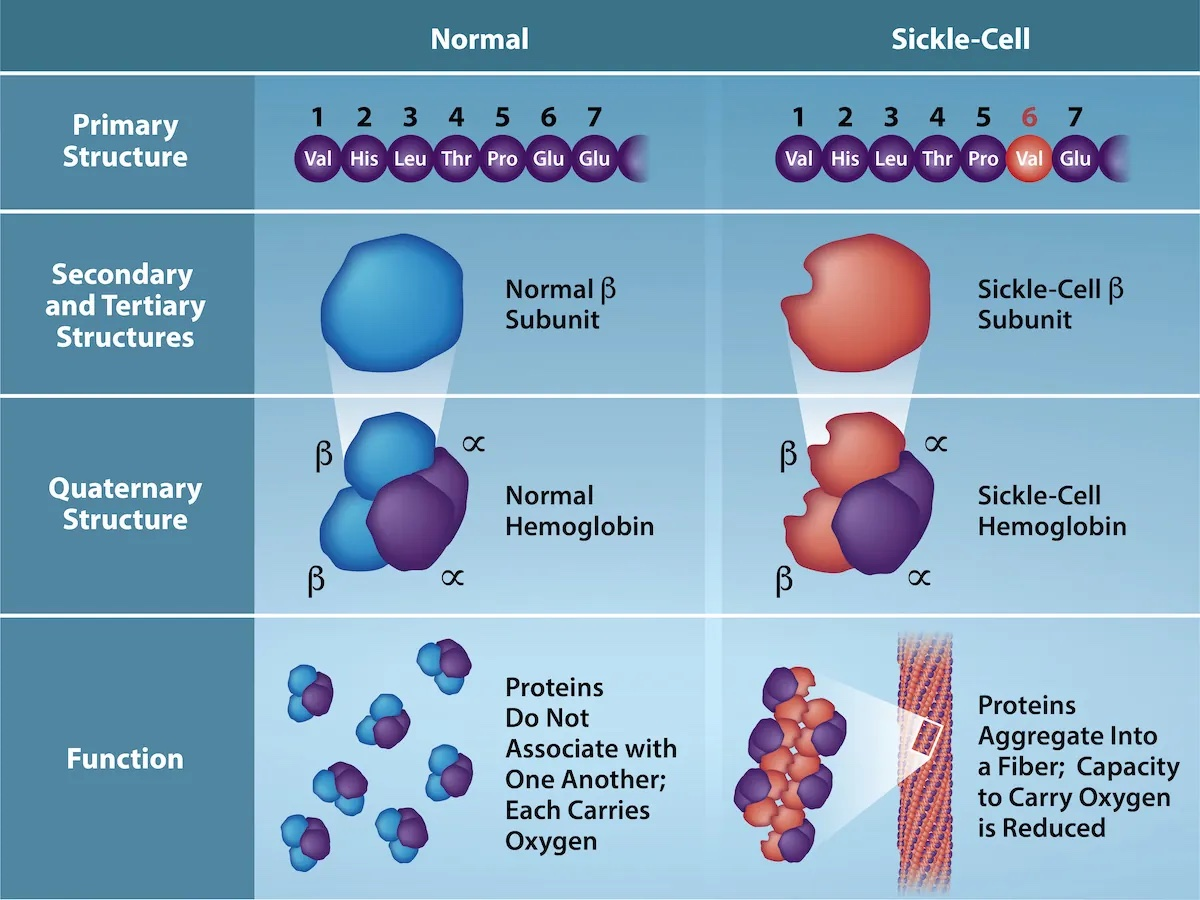
\includegraphics[width=0.7\linewidth]{files/sicklecell-9c221211df6604b37609733b9d82c043.jpg}
\caption[]{Consequences of a substitution in hemoglobin $\beta$ resulting in sickle cell anemia.
Credits: Rao, A., Tag, A. Ryan, K. and Fletcher, S. Department of Biology, Texas A\&M University.}
\label{sicklecell}
\end{figure}

% #% Figure sicklecell is credited but the image is not found on a specific webpage. Is showing credits enough? - Similar to Pearson imagery (Campbell Biology 11th edition Figure 5.19).


\bigskip
\centerline{\rule{13cm}{0.4pt}}
\bigskip

\subparagraph{Visualization}

There are many styles to view protein molecular structures. Some styles focus on detailed chemical structure, others are targeted at the protein surface.
For some examples see Figure~\ref{protrep}.

\begin{figure}[!htbp]
\centering
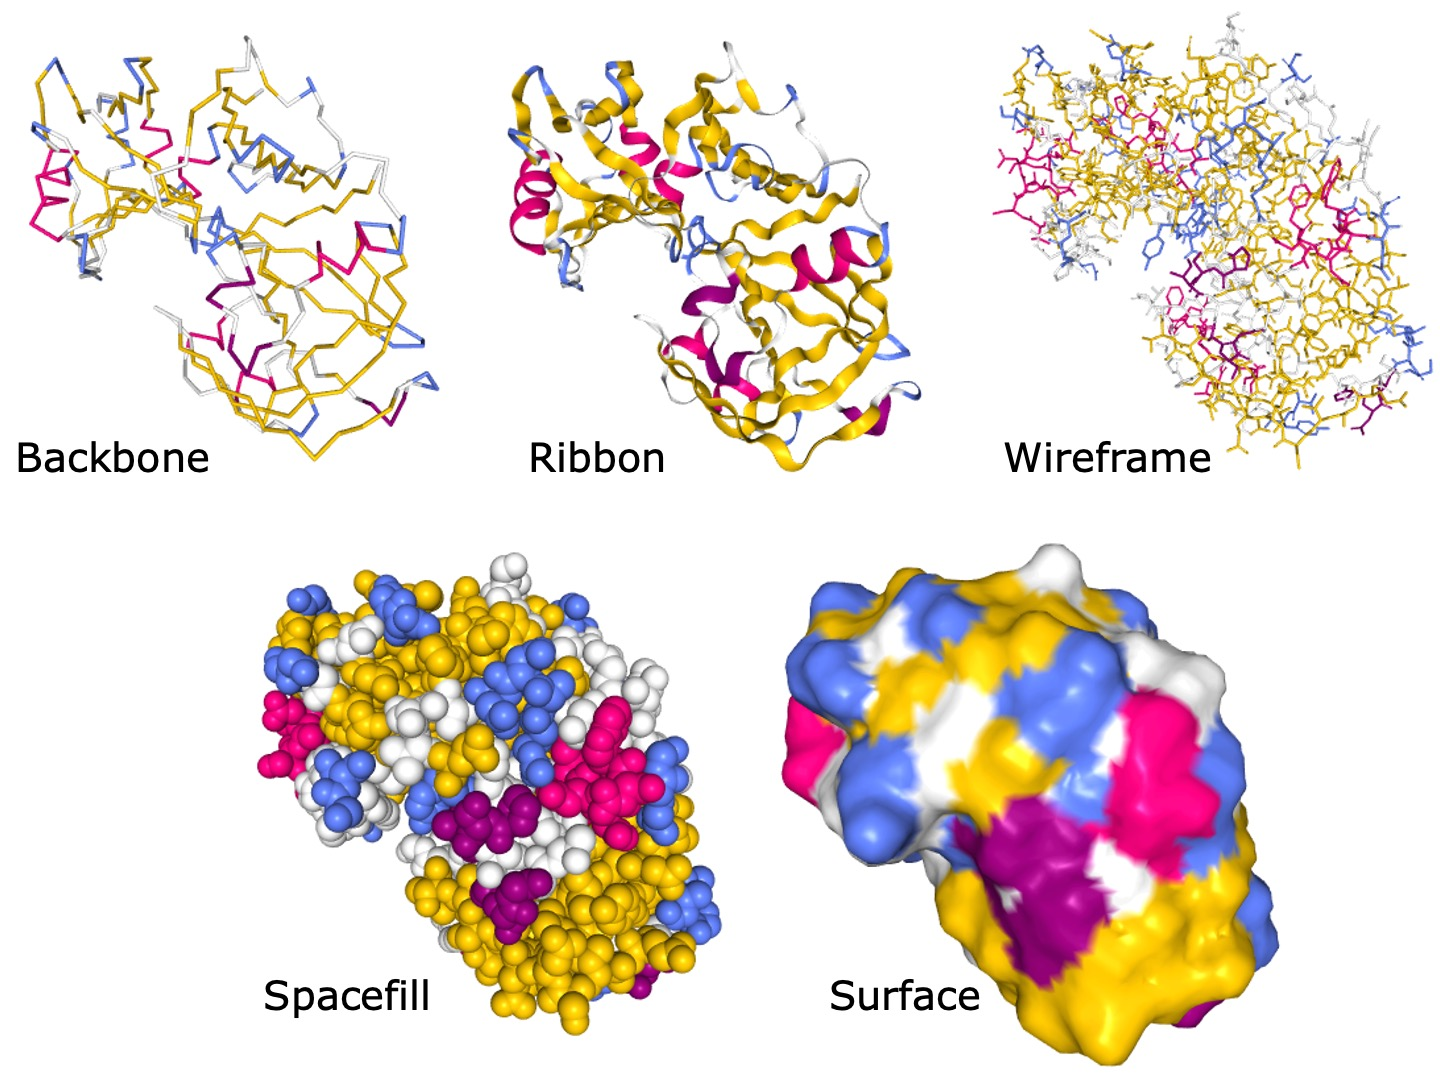
\includegraphics[width=0.6\linewidth]{files/protrep-dbcbffe70f8b8a99767b7579c1bd83d0.jpg}
\caption[]{Different representations of the PDB structure 5PEP generated with NGL. Credits: \citet{rcsb_2000, protrep_1990, ngl_2018}.}
\label{protrep}
\end{figure}

% #% The citation above does not end up in alphabetical order. This is probably caused by ngl_2018 being referenced earlier in the markdown than protrep_1990. Not sure how to fix without adopting a custom inline citation reference style.

\begin{framed}
\textbf{See Also}\\
Most of the figures in this section are taken from \href{https://openstax.org/books/biology-2e/pages/3-4-proteins}{OpenStax}, where you can also find more information on proteins.
\end{framed}


\bigskip
\centerline{\rule{13cm}{0.4pt}}
\bigskip

\subsubsection{Genome annotation}\label{chapter1_genome_annotation}

Genome annotation is the process of deciphering what information is encoded in an organism's DNA.
It is an ongoing effort in organisms with known genome sequences.
Even moreso, genome annotation is a critical step in acquiring biological insights from newly sequenced genomes.
Given the large size of any genome, automated procedures are used to identify various genomic elements such as genes, regulatory regions, transposable elements, or other non-coding elements.
Each of these bioinformatic procedures typically focuses on identifying one type of element, and as such a complete genome annotation project can be thought of as a pipeline of various procedures.
The following section describes the most common steps in genome annotation.

\begin{framed}
\textbf{Note 1.4: Alignment algorithms}\\
Several steps in the genome annotation process make use of algorithms that can search or align biological sequences, for example the BLAST algorithm.
\href{/chapter2}{Chapter 2} covers sequence alignment and search in greater detail.
For now, it is sufficient to know that these algorithms can quickly search very large collections of biological sequences to identify sequences that look similar (what we mean \textit{exactly} by `similar' is also part of \href{/chapter2}{chapter 2}).
\end{framed}

\paragraph{Repeat masking}\label{Chapter1_repeat_masking}

Repeat masking involves the identification and masking (hiding) of repetitive sequences within a genome.
It is an essential first step in annotating most genomes because repetitive sequences can pose significant challenges in genome annotation.
Masking repeats generally improves:

\begin{itemize}
\item Accuracy: repetitive elements can be mistakenly annotated as genes or other functional elements, leading to inaccurate predictions and interpretations of the genome.
\item Computational efficiency: identifying and processing repetitive sequences can be computationally intensive.
However, masking these repetitive regions reduces the computation time of all downstream analyses.
\item Biological relevance: repetitive sequences are usually not involved in the coding of proteins of interest.
Therefore, focusing on non-repetitive regions is a smart choice in understanding the genes and regulatory elements that drive biological processes.
\end{itemize}

Most repeat masking workflows work by first compiling (or using a precompiled) `repeat library': a collection of known repetitive elements that have previously been characterized.
Subsequently, the genome to be annotated is compared against this repeat library using various computational algorithms, such as BLAST or RepeatMasker.
When a match is found, the corresponding region in the genome is `masked' or annotated as a repetitive element.
This means that these regions are excluded from further analysis or labeled as repetitive.

\paragraph{Gene prediction}\label{Chapter1_gene_prediction}

The process of finding protein coding genes differs between prokaryotic and eukaryotic genomes.
In both cases the aim is to find open reading frames (ORFs): contiguous stretches of DNA that encode proteins.
However, since RNA splicing (Figure~\ref{splicing}) is almost absent in prokaryotic genomes, prokaryotic ORFs can be found directly in the genomic DNA.
As a result, simply enumerating all possible ORFs in a genome is a common step in prokaryotic genome annotation.
In contrast, ORFs in eukaryotic genomes are found on \textit{mature} mRNAs. As such, all eukaryotic gene prediction methods take splicing into account, thereby greatly increasing their computational complexity.
Both prokaryotic and eukaryotic gene prediction typically can be classified as either evidence based prediction or ab initio prediction, both will be explained below.

\subparagraph{Evidence based prediction}

This data-driven approach uses existing and newly generated data to get hints on what regions of a genome encode genes.
Depending on the type of data, these predictions have more or less predictive power.
Some commonly used evidence types are:

\begin{itemize}
\item RNA-sequencing data: the most direct form of evidence for what regions of the genome are transcribed.
As such, RNA-sequencing (often abbreviated to RNA-seq) `reads' often provide the best form of evidence in identifying splice sites in eukaryotes.
Note that not all transcribed RNA will be translated into proteins, and that therefore not all RNA-sequencing reads are evidence for protein coding genes.
Distinguishing between protein-coding and non-coding RNA is not always trivial.
\item Homology evidence: Aligning DNA or protein sequences of known genes (from other organisms) is valuable evidence in finding coding regions of the genome.
Due to the redundancy in the genetic code, it is not trivial to correctly identify splice sites when aligning protein sequences to a genome.
Homology evidence from closely related organisms leads to higher quality predictions than evidence from distantly related organisms.
\item Whole-genome alignments: this approach uses the annotated genome of a closely related organism to directly identify coding regions in a novel genome.
For example: whole-genome alignment of mouse and human genomes reveals that large parts of mouse chromosome 2 are homologous to human chromosome 20.
The alignment procedure results in a direct 1-to-1 mapping of mouse and human genome coordinates, and as such annotation coordinates can be transferred between genomes.
\end{itemize}

\subparagraph{Ab initio prediction}

\begin{quote}
\textit{Ab initio} (latin): from first principles, from the beginning
\end{quote}

These methods rely on statistics to learn a predictive model from a known annotated genome.
Various forms of ab initio models exist, and whereas implementation details differ, most follow a similar line of reasoning.
For now, we will stick to a high level description.
All ab initio models scan through a DNA sequence and at each position give a score for a specific type of annotation.
In addition, they often take their genomic context into account.
For example, the probability of a protein-coding annotation on a nucleotide A is high when the next two observed nucleotides are T and G, producing the ATG start-codon methionine.
In addition, most methods also take the \textit{predicted annotation} of the genomic context into account.
For example: the probibility that ATG actually codes for a start codon is much higher if we can predict an in-frame stop codon.
In eukaryotic genome prediction these models become quite complex because they have to include splice sites in all three reading frames.
How \textit{exactly} a model decides what annotation score to give to which nucleotide is part of the model architecture and parameterization.
In all cases, the model parameters are chosen to accurately reproduce a known genome annotation.
If sufficient data is used to learn the model parameters, it is assumed that these models can be used to predict annotations on novel genome sequences.
Like homology-based prediction, this model-based approach works best for closely related organisms. In the past, almost all ab initio prediction methods were formulated as hidden Markov models (HMMs) (see Note 1.5). Examples of tools implementing HMM based ab initio prediction are SNAP, GeneMark, and Augustus. With the availability of more high quality data (genome sequences and accompanying annotations), approaches based on deep learning and generative AI have proven to frequently perform better than HMM based approaches.

\begin{framed}
\textbf{Note 1.5: Hidden Markov models (HMMs)}\\
Hidden Markov models (HMMs) are useful for the statistical modelling of general sequence characteristics. As such they find widespread adoption in bioinformatics to study biological sequences. Providing a full technical description of all aspects of HMMs is outside of the scope of this book. Here we will stick to a somewhat simplistic description to provide a first introduction.

A hidden Markov model can be used to predict some unobserved labelling across a sequence of observations. For example: in genome annotation, coding and non-coding regions of a genome can be treated as an unobserved characteristic, where the nucleotides are the sequence of observations. As such, `hidden' refers to the \textit{unobserved labelling}. In addition, `Markov' refers to some useful statistical assumptions on the nature of independence between observations and labellings that enable efficient computation.

More formally, the unobserved labellings are referred to as the `hidden states', and every hidden state contains some probabilities of observing our sequence of interest, called the `emission probabilities'. To complete our HMM definition, we define `transition probabilities' between hidden states.

The combination of hidden states, emission probabilities, and transition probabilities enable asking questions such as `given my current observation and a certain label of my previous observation, what is the most likely label for my current observation?'. In the context of genome annotation this would translate to for example `given that I see a stop-codon, and that my previous label was coding sequence, what is my current most likely label?', the answer to which would be `non-coding' (See Figure~\ref{coding_hmm}).

\begin{figure}[!htbp]
\centering
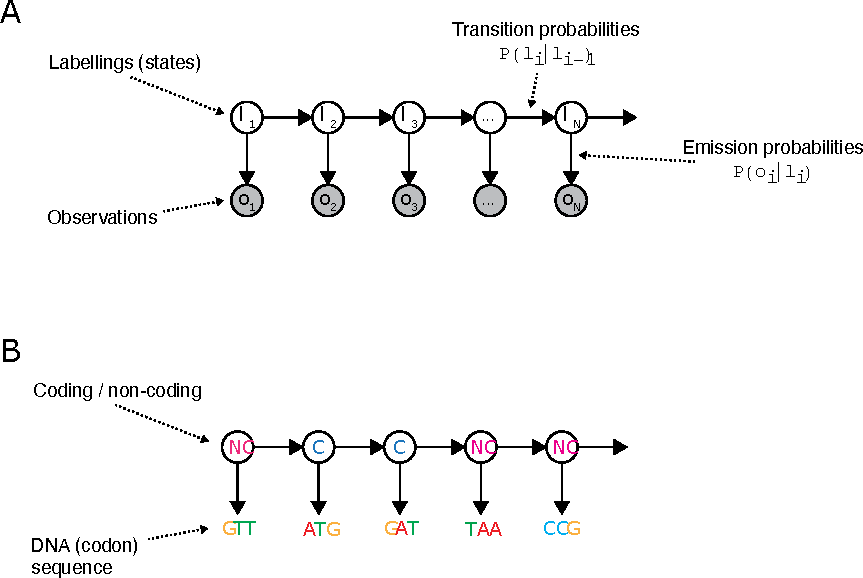
\includegraphics[width=1\linewidth]{files/coding_hmm-22db191de15f76bd6deb9e5904ea2580.pdf}
\caption[]{\textbf{A}: Graphical representation of a general hidden Markov model. Shaded circles indicate observations, white circles indicate unobserved labellings (hidden states). Black arrows indicate transition probabilities between hidden states, and emission probabilies for observations from hidden states. Note that there are no arrows between observations! This is one of the properties of HMMs that enable efficient computation. \textbf{B}: A (simplified) HMM variant that labels a sequence of DNA codons as either coding or non-coding. Real-world gene predicition HMMs use a more elaborate structure with more hidden states, and six-frame representations of the DNA.
Credits: \href{https://creativecommons.org/licenses/by-nc/4.0/}{CC BY-NC 4.0} \cite{own_1_2024}.}
\label{coding_hmm}
\end{figure}

\href{/chapter2}{Chapter 2} and \href{/chapter4}{Chapter 4} cover various other applications of HMMs in bioinformatics, such as defining and prediction sequence domains, or transmembrane properties of proteins.
\end{framed}

\paragraph{Evidence/prediction integration}

From the previous sections it has now become clear there are several ways of predicting what the genes in a genome look like.
Since these various approaches almost never agree exactly in their predictions, a final step in genome annotation is evidence and prediction integration.
Typically a weighted consensus approach is used: each individual source of evidence is given a weight representing how much it should influence the final decision, after which a majority vote decides what the annotation should look like.
Typically RNA-seq evidence gets a high weight, and various forms of homology evidence can be weighted depending on how closely related they are to the genome of interest.

\paragraph{Functional annotation}\label{chapter1_functional_annotation}

So far, all described steps in the genome annotation process have dealt with what genes look like on a structural level.
To gain biological insight, the next step is to assign functional annotations to the predicted genes.
This functional annotation step consists of using various sequence alignment and search tools to find sequences with a known function/description and to transfer the information of the known gene to the predicted gene.
Several databases of high-quality known functions are often used, which are described in more detail in the next section of this chapter.
In Chapter~2 we will learn about approaches how to search these databases efficiently.

\begin{framed}
\textbf{Note 1.6: Visualizing gene structure}\\
\textbf{Gene models}: the genomic structure of a gene (often referred to as a gene `model') is typically visualized by a set of lines and rectangles with predefined meaning.

\begin{figure}[!htbp]
\centering
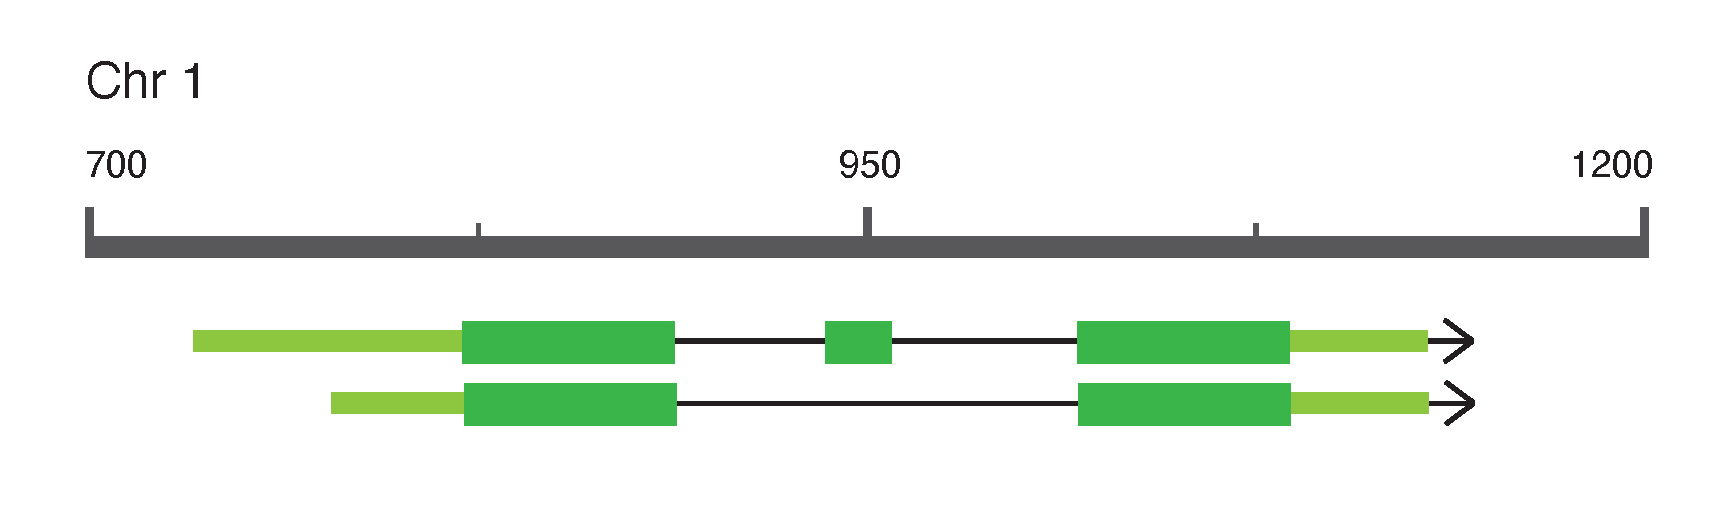
\includegraphics[width=1\linewidth]{files/genemodel-7bb5f6683cb808b770f42927d7e7aacb.png}
\caption[]{An example gene model.
Various visualization conventions can be identified: boxes represent genomic regions that are transcribed.
Boxes are exons, lines between boxes are introns. Narrow boxes (sometimes with a lighter color) are untranscribed regions (UTRs), wider boxes (sometimes darker colored) are coding sequence regions (CDS).
The arrow indicates the direction of transcription.
In this example a gene on chromosome 1 with two splice variants is shown, where the first variant has a slightly longer 5' UTR and an additional CDS exon in between the first and last exons.
Credits: \href{https://creativecommons.org/licenses/by-nc/4.0/}{CC BY-NC 4.0} \cite{own_1_2024}.}
\label{genemodel}
\end{figure}

\textbf{Genome browsers} facilitate interactive visualization of annotations and evidence alignments on genome sequences.
Various implementations exist, but all genome browsers typically provide a linear view of a chromosome that can be scrolled and zoomed.
In addition, various annotation `tracks' can often be toggled, to display for instance known gene structures, RNA sequencing alignments, or homologous protein sequence alignments.
Most visualization elements can be clicked to open pop-up windows with additional information.

\begin{figure}[!htbp]
\centering
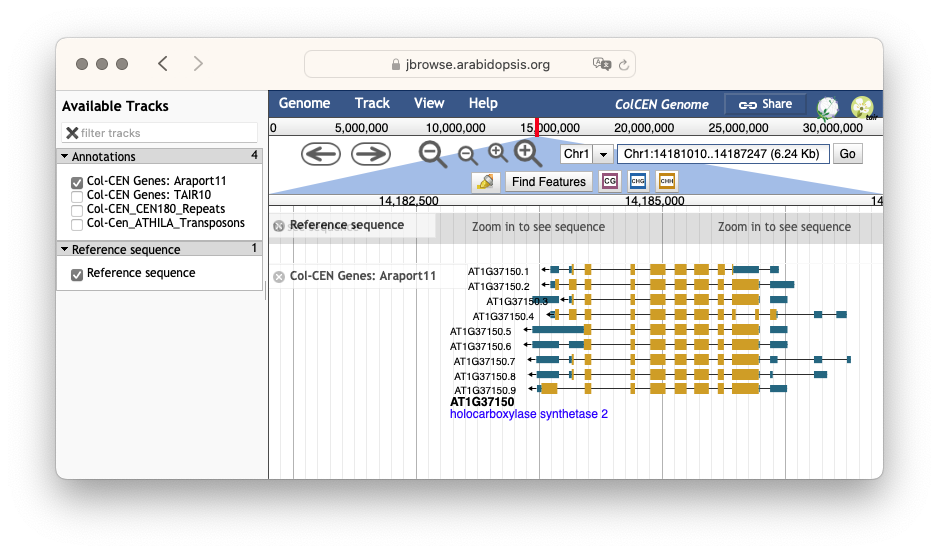
\includegraphics[width=1\linewidth]{files/jbrowse-54f15198e78cd826afaaf0266ba943cb.png}
\caption[]{A screenshot of the JBrowse genome browser showing \textit{Arabidopsis thaliana} chromosome 1 with a gene that has multiple splice variants. Credits: \cite{jbrowse_2016}.}
\label{jbrowse}
\end{figure}
\end{framed}


\bigskip
\centerline{\rule{13cm}{0.4pt}}
\bigskip

\subsubsection{Databases}\label{chapter1_databases}

\paragraph{Introduction}

Databases are at the core of bioinformatics.
In all analyses, we integrate pre-existing data and we need to access this data.
The journal Nucleic Acids Research publishes an entire issue in the beginning of each year on new and updated databases.
The list of these databases can also be accessed \href{https://www.oxfordjournals.org/nar/database/c}{online}.

Computer scientists have developed different kinds of databases.
One example are relational databases, which can be queried by \textbf{SQL} (structured query language) and which perform well for data that is processed computationally.
Another example are \textbf{XML} (extended markup language) databases which store data in specified well-structured XML files.
Nevertheless, most databases for biological sequence data use \textbf{flat file databases}, where the data is saved in structured text files.
This data can be manipulated in a text editor without requiring an additional program for database management, and they can be easily exchanged between scientists.
On the downside, searching them has a lower performance.
This is why they are often indexed, i.e., they contain an \textbf{index} of keywords, similar to a glossary in a book.

Depending on the kind of data included, we distinguish different kinds of biological databases:

\begin{itemize}
\item \textbf{Primary databases} contain primary sequence information from experimentally derived data that is directly submitted by the scientists that generated the data.
\item \textbf{Secondary databases} provide the results of analyses of the information in primary databases.
\end{itemize}

Each entry in a database has a unique \textbf{accession number}.
This number is permanent and provides an unambiguous way to link to the entry.
The information that the accession refers to should not change.
To still allow updates to an entry, the accession number can contain a \textbf{version}, usually after a dot.
For example, NC\_003070.9 is the latest version (version 9) for \textit{Arabidopsis thaliana} chromosome 1 in RefSeq.

Database entries often link to each other via \textbf{cross links}.

\begin{framed}
\textbf{See Also}\\
\href{https://www.ncbi.nlm.nih.gov/pmc/articles/PMC5104318/}{Ten Simple Rules for Developing Public Biological Databases} contains additional reading material on what it takes to properly maintain a public database service.
\end{framed}


\bigskip
\centerline{\rule{13cm}{0.4pt}}
\bigskip

\paragraph{GenBank}

\href{https://www.ncbi.nlm.nih.gov/genbank/}{GenBank} is a popular primary database for nucleotide sequences and is based at the \href{https://www.ncbi.nlm.nih.gov/}{NCBI} (National Center for Biotechnology Information).
A GenBank release usually occurs every two months and the most recent \href{https://www.ncbi.nlm.nih.gov/genbank/release/current/}{release} from the 15\textsuperscript{th} of December 2023 contains {\textasciitilde}250 million sequences and additionally {\textasciitilde}3.7 billion WGS (whole genome shotgun) records.
The latter are genome assemblies or genomes that were not yet completed.
The complete database is available for download via FTP, but the most convenient way to access individual entries is via the search on the GenBank website (Figure~\ref{genbank_figure}).

\begin{figure}[!htbp]
\centering
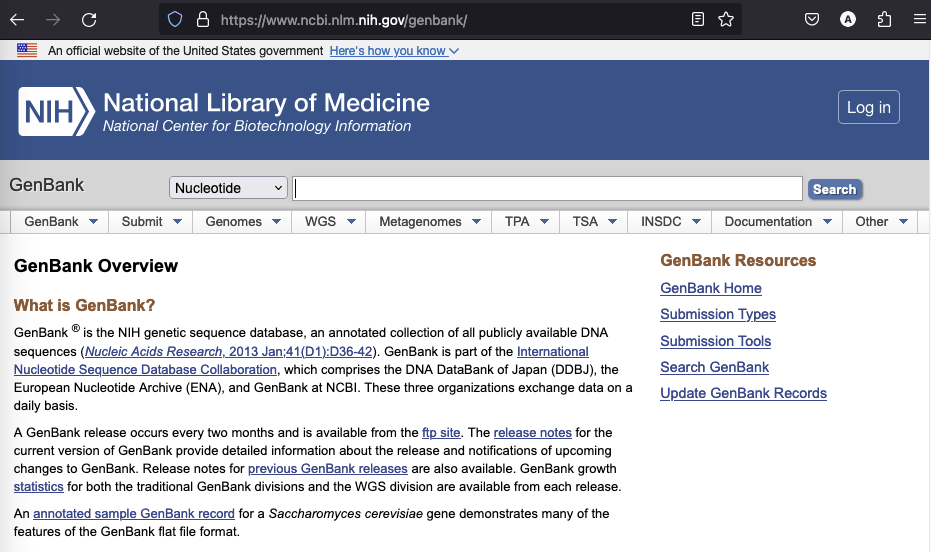
\includegraphics[width=1\linewidth]{files/genbank-f7d7daa5982bc401e1c7f56159ba59fb.png}
\caption[]{A screenshot of the GenBank website. Credits: \cite{genbank_2012}.}
\label{genbank_figure}
\end{figure}

\begin{framed}
\textbf{Additional information}\\
These days, it is required for publication in most peer-reviewed journals that scientists submit their sequence data to GenBank or an associated database, alongside sufficiently informative meta-data that describes how the data was generated.
\end{framed}

Since data is directly submitted to GenBank, the information for some loci can be highly redundant.
The sequence records are owned by the original submitter and cannot be altered by someone else.

\begin{framed}
\textbf{Note 1.7: Database redundancy}\\
`Redundancy' in the context of a database refers to identical data that is present more than once.
Typically, \textit{metadata} is not taken into account when determining redundancy.
Example: two different labs have determined the DNA sequence of a bacterial gene involved in some disease.
The metadata will be different, but the sequence data will be identical, so these two database records are redundant.

NCBI hosts several databases that are classified as `non-redundant', for example \href{https://www.ncbi.nlm.nih.gov/refseq/about/nonredundantproteins/}{RefSeq non-redundant proteins}.
Here, redundancy is defined so that a `non-redundant protein record always represents one exact sequence that has been observed once or many times in different strains or species'.
\end{framed}

Genbank is part of the \href{https://www.insdc.org/}{INSDC} (International Nucleotide Sequence Database Collaboration).
The other two member databases are \href{https://www.ebi.ac.uk/ena/browser/home}{ENA} (European Nucleotide Archive) and \href{https://www.ddbj.nig.ac.jp/index-e.html}{DDBJ} (DNA Data Bank of Japan).
The data submitted to either database is exchanged daily, so all databases contain essentially the same information.


\bigskip
\centerline{\rule{13cm}{0.4pt}}
\bigskip

\paragraph{RefSeq}

The Reference Sequence (\href{https://www.ncbi.nlm.nih.gov/refseq/}{RefSeq}) collection is also hosted at NCBI and contains genomic DNA, transcripts, and proteins.
The aim of RefSeq is to provide non-redundant, curated data.
RefSeq genomes are copies of selected assembled genomes in GenBank.
Additionally, transcript and protein records are generated by several processes:

\begin{itemize}
\item Computation via the \href{https://www.ncbi.nlm.nih.gov/genome/annotation\_euk/}{eukaryotic} or \href{https://www.ncbi.nlm.nih.gov/genome/annotation\_prok/}{prokaryotic} annotation pipeline.
\item Manual curation.
\item Transfer of information from annotated genomes in GenBank.
% #% The eukaryotic and prokaryotic RefSeq links lead to soon to be redundant pages. Not sure what to replace this with.

In contrast to GenBank, RefSeq records are owned by NCBI and can be updated to maintain annotation.
The current release is 222 from the 8\textsuperscript{th} of January 2024 and contains {\textasciitilde}305 million proteins from {\textasciitilde}145,000 organisms.
\end{itemize}

The RefSeq accessions directly provide information on \href{https://www.ncbi.nlm.nih.gov/books/NBK21091/table/ch18.T.refseq\_accession\_numbers\_and\_mole/?report=objectonly}{molecule types}.
For example, \texttt{NC\_} accessions denote complete genomes, \texttt{NP\_} accessions denote proteins in one genome, and \texttt{WP\_} accessions denote proteins in multiple genomes.


\bigskip
\centerline{\rule{13cm}{0.4pt}}
\bigskip

\paragraph{UniProt}\label{chapter1_uniprot}

There is lots of information available for proteins, such as sequence information, domains, expression, or 3D structure.
The aim of the Universal Protein Resource (\href{https://www.uniprot.org/}{UniProt}) is to provide a comprehensive resource for proteins and their annotation.
UniProt contains three databases (Figure~\ref{uniprot}):

\begin{itemize}
\item UniProt Knowledgebase (UniProtKB) - see below.
\item UniProt Reference Clusters (\href{https://www.uniprot.org/help/uniref}{UniRef} - clusters of protein sequences at 100\%, 90\%, and 50\% identity.
\item UniProt Archive (\href{https://www.uniprot.org/help/uniparc}{UniParc} - non-redundant archive of publicly available protein sequences seen across different databases.
\end{itemize}

\begin{figure}[!htbp]
\centering
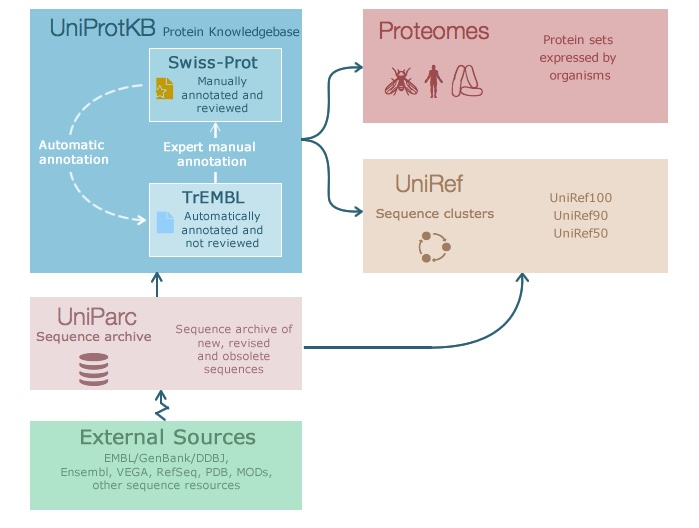
\includegraphics[width=0.7\linewidth]{files/uniprot-93dd5f84ee9208207fa0fe44b574d65a.jpg}
\caption[]{The information flow in Uniprot.
Credits: \href{https://creativecommons.org/licenses/by-nc-nd/4.0/}{CC BY-NC-ND 4.0} \cite{uniprot_2021}.}
\label{uniprot}
\end{figure}

\textbf{UniProtKB} is the central hub for functional information on proteins.
For each protein it contains the core data (such as sequence, name, description, taxonomy, citation) and as much annotation information as possible.
It contains many cross-references to other databases and is generally a very good starting point to find information on a protein.

UniProtKB consists of two sections:

\begin{itemize}
\item \href{https://web.expasy.org/docs/userman.html\#what\_is\_sprot}{Swiss-Prot} - manually-annotated records with information extracted from literature and curated computational analysis.
\item \href{https://web.expasy.org/docs/userman.html\#what\_is\_trembl}{TrEMBL} - automatically annotated records that are not reviewed.
\end{itemize}

UniProtKB is updated every 8 weeks. The current release has {\textasciitilde}570,000 entries in Swiss-Prot and {\textasciitilde}248 million entries in TrEMBL.


\bigskip
\centerline{\rule{13cm}{0.4pt}}
\bigskip

\paragraph{Prosite}\label{chapter1_prosite}

\href{https://prosite.expasy.org/}{Prosite} is a secondary database of protein domains, families, and functional sites.
Some regions in protein families are more conserved than others because they are important for the structure or function of the protein.
Prosite contains motifs and profiles specific for many protein families or domains.
Searching motifs in new proteins can provide a first hint for protein function.

The current release of Prosite from the 24\textsuperscript{th} of January 2024 contains 1311 patterns, 1386 profiles, and 1400 ProRule entries.

A Prosite \textbf{pattern} is typically 10 to 20 amino acids in length.
These short patterns are usually located in short well-conserved regions, such as catalytic sites in enzymes or binding sites.
A pattern is represented as a regular expression, where amino acids are separated by hyphens and \texttt{x} denotes any letter.
Repetitions can also be given as the number of repetitions in brackets.
For example, \texttt{[AC]-x-V-x(4)-\{ED\}} matches sequences that contain the following amino acid sequence: Ala or Cys-any-Val-any-any-any-any-any but Glu or Asp.
Note that this representation is \textbf{qualitative}, a sequence either matches a pattern or it does not.

Patterns cannot deal with mismatches and are limited to exact matches to the pattern.
Thus, they are not well suited to identify distant homologs.
A Prosite \textbf{profile} is more general than a pattern and can also detect poorly conserved domains or families.
They characterize protein domains over their entire length and do not just model the conserved parts.
Profiles are estimated from multiple sequence alignments and we learn more about them in \href{/chapter2}{chapter 2}.
For now, it is important to know that profiles model matches, insertions, and deletions.
Importantly, profiles are \textbf{quantitative} representations, they will return a score how well the sequence fits to the profile.
A threshold can be applied to get high-scoring profiles for a sequence.
In contrast to patterns, a mismatch to a profile can be accepted if the rest of the sequence is highly similar to the profile.
Profiles are well suited to model structure properties of a domain.

Notably, profiles cover the structural relationships of domains, but they might also score a sequence highly that lacks important functional residues.
To include that information, \textbf{ProRule} contains additional information about Prosite profiles, such as the position of structurally or functionally important amino acids.
ProRule is used to guide curated annotation of UniProtKB/Swiss-Prot.

\paragraph{InterPro}\label{chapter1_interpro}

The Integrated Resource of Protein Families, Domains and Sites (\href{https://www.ebi.ac.uk/interpro/}{InterPro}) integrates 13 member databases (including Prosite and Pfam) into a comprehensive secondary database.
Additionally, it provides annotation from other tools, for example to annotate signal peptides and transmembrane regions.
It allows to identify functionally important domains and conserved sites in a sequence by simultaneously annotating it using the member databases.
Interpro can be used to find out which protein family a sequence belongs to, or what its putative function is.
Additionally, one InterPro entry can integrate entries from the member databases, if they represent the same biological entity, reducing redundancy.
InterPro entries are also linked to Gene~Ontology.
They are curated before being released.

InterPro is updated every 8 weeks. The current release from the 25\textsuperscript{th} of January 2024 contains {\textasciitilde}41,000 entries, which represent different types:

As an example, look at the \href{https://www.ebi.ac.uk/interpro/entry/InterPro/IPR010945/}{InterPro entry} for the type 2 malate dehydrogenase protein family.
The entry has a name (malate dehydrogenase, type 2) and accession (IPR010945).
The contributing entries in member databases are shown on the right-hand side, with links to the individual member database entries.
A descriptive abstract explains what these proteins are and what their function is.
A set of GO terms is also provided, which describe the characteristics of the proteins matched by the entry.

You can get the InterPro annotation for a protein by running a new sequence search (Figure~\ref{interpro-search}), or by by looking up its UniProt accession (Figure~\ref{interpro-browse}).

\begin{figure}[!htbp]
\centering
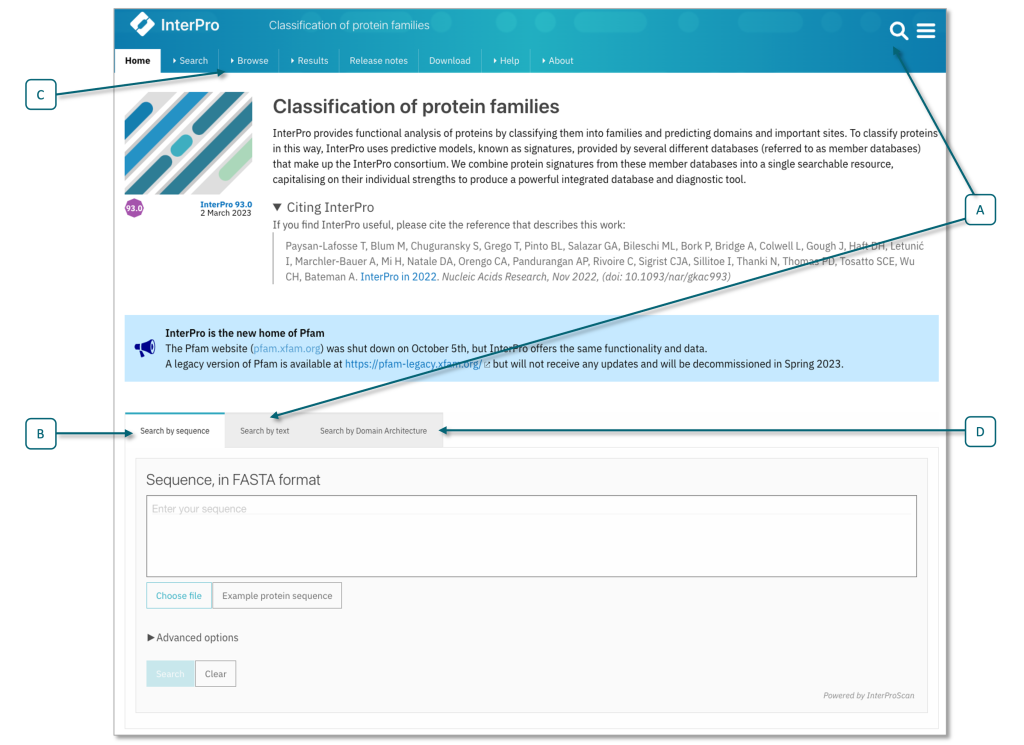
\includegraphics[width=1\linewidth]{files/interpro-search-6c154991474b34bbe8ce014cfbd76ce3.png}
\caption[]{Search fields on the InterPro home page, showing text search field (A) and the sequence search (B) options, including `Advanced options', where you can limit your search to member databases or sequence features of interest.
Selecting the browse tab in the top menu (C) allows access to a browse search, (e.g., search for member database signature, InterPro entry type), see also Figure~\ref{interpro-browse}.
You can also search for a particular domain architecture (D).
Credits: \cite{interpro_2022}.}
\label{interpro-search}
\end{figure}

\begin{figure}[!htbp]
\centering
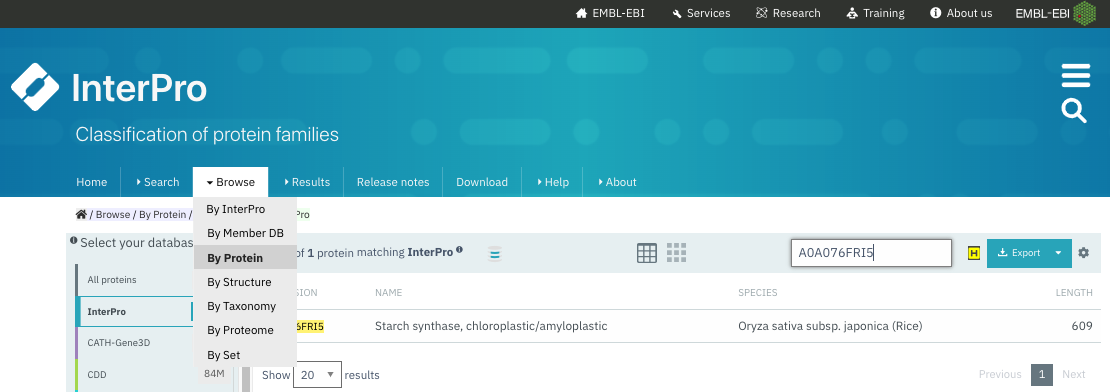
\includegraphics[width=1\linewidth]{files/interpro-browse-1ae9c2adc4608445ebe1acc3eca4156e.png}
\caption[]{Browse the annotated proteins in Interpro and search for a UniProt accession.
See resulting entry in (Figure~\ref{interpro-prot}). Credits: \cite{interpro_2022}.}
\label{interpro-browse}
\end{figure}

\begin{figure}[!htbp]
\centering
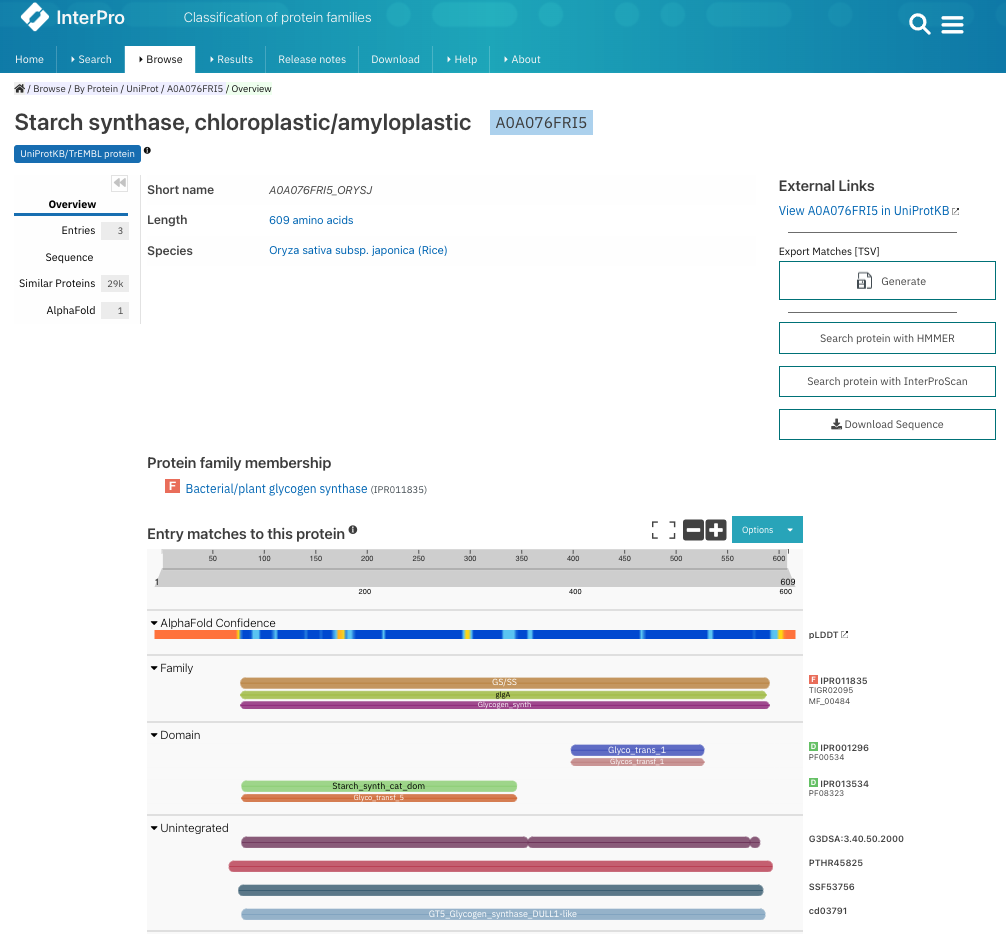
\includegraphics[width=1\linewidth]{files/interpro-prot-21d5398cff123b16fdb878429744a14e.png}
\caption[]{The result page when looking up UniProt accession \href{https://www.ebi.ac.uk/interpro/protein/UniProt/A0A076FRI5/}{A0A076FRI5} in InterPro.
You can see the family and domain annotation and on the right the accessions in InterPro and in the member databases.
You can click on each of these accessions to get to the entry information. Credits: \cite{interpro_2022}.}
\label{interpro-prot}
\end{figure}

You may have noticed a colored letter before each InterPro accession, e.g., F before IPR011835 or D before IPR001296 (Figure~\ref{interpro-prot}).
These icons denote the different InterPro entry types:

\begin{itemize}
\item (Homologous) Superfamily - a large diverse family, usually with shared protein structure.
\item Family - a group of proteins sharing a common evolutionary origin, reflected by their related functions and similarities in sequence or structure.
\item Domain - a distinct functional or structural unit in a protein, usually responsible for a particular function or interaction.
\item Repeat - typically a short amino acid sequence that is repeated within a protein.
\item Site - a group of amino acids with certain characteristics that may be important for protein function, e.g., active sites or binding sites
\end{itemize}

\begin{figure}[!htbp]
\centering

\includegraphics[width=0.4\linewidth]{files/interpro-types-5f7c10e9e25c86c696214d3eeac1e545.png}
\caption[]{The icons for the different InterPro entries (homologous superfamily, family, domain, repeat or site).
Credits: \href{https://creativecommons.org/licenses/by-sa/4.0/}{CC BY-SA 4.0} \cite{interpro-types_2020}.}
\label{interpro-types}
\end{figure}

\begin{framed}
\textbf{See Also}\\
You can find more information on InterPro entry types with examples \href{https://www.ebi.ac.uk/training/online/courses/interpro-functional-and-structural-analysis/what-is-an-interpro-entry/interpro-entry-types/}{here}.
\end{framed}

\paragraph{Pfam}\label{chapter1_pfam}

Pfam is an important resource for protein domains.
In Pfam, domains are classified according to profiles that are modelled as Hidden Markov models (HMMs).
We will learn more on HMMs in \href{/chapter2}{chapter 2}.

% #% Create a direct cross-link to HMMs in chapter 2 when written.

Pfam is now integrated in InterPro.
Each Pfam domain can be represented with a logo, where the amino acids frequent at a particular position are represented as larger letters (Figure~\ref{pfam-profile}).

\begin{figure}[!htbp]
\centering
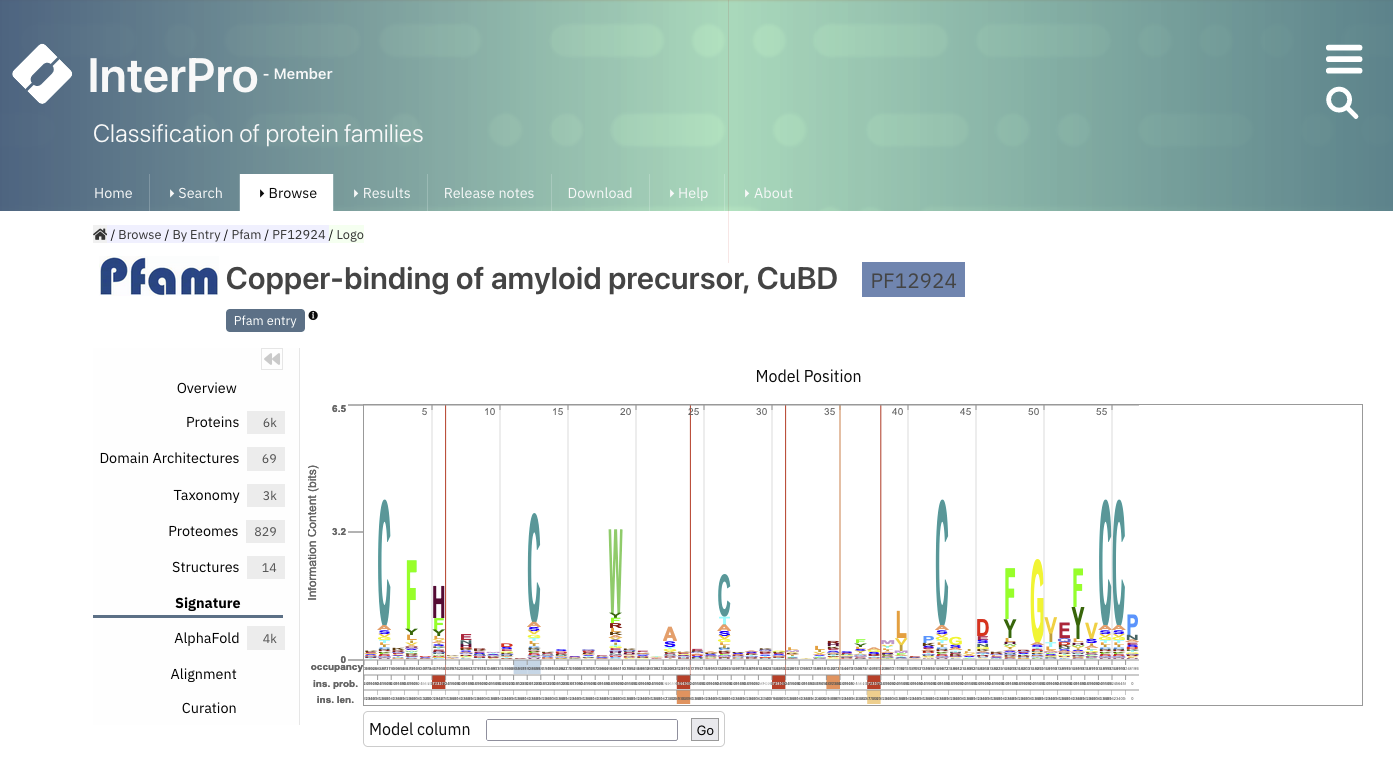
\includegraphics[width=0.7\linewidth]{files/pfam-profile-46bb7a5320328b531204cc524a214845.png}
\caption[]{The Pfam logo for PF12924.
Credits: \cite{interpro_2022}.}
\label{pfam-profile}
\end{figure}


\bigskip
\centerline{\rule{13cm}{0.4pt}}
\bigskip

\paragraph{File formats}

There are many different formats for biological data.
A format is a set of rules about the contents and organization of the data.
You should be familiar with a couple of common data formats in bioinformatics, which you will experience in the practicals.

\begin{framed}
\textbf{Note 1.8: Examples of common data formats in bioinformatics}\\
\begin{itemize}
\item FASTA
\item Genbank
\item GFF (Generic Feature Format)
\item FASTQ
\item SAM/BAM (Sequence Alignment/Map format)
\item VCF (Variant Call Format)
\item PDB (structure data)
\end{itemize}
\end{framed}

\subparagraph{Plain text files}

Many of the biological data formats are plain text files, they only contain letters, numbers, and symbols, but no formatting, such as font size or colors.
As a convention, they usually have the ending \texttt{.txt}.
The advantage of plain text files is that they can be opened with any text editor on any computer.
Plain text differs from rich text format, where the latter can also include formatting.
Many bioinformatics programs expect plain text files as input.
Thus, when creating them on your computer, take care to save in this format, and not for example in rtf or word.

On a Windows computer, plain text files can for example be created with the Notepad program (Figure~\ref{notepad}).

\begin{figure}[!htbp]
\centering
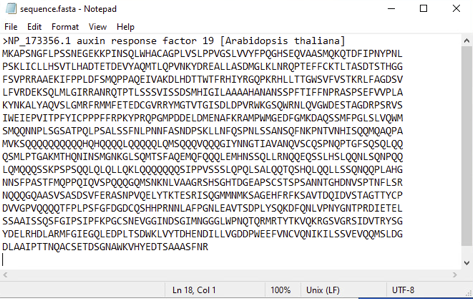
\includegraphics[width=0.7\linewidth]{files/notepad-5b8ceca90dcca4116236b117fb2fa376.png}
\caption[]{A screenshot of Notepad on Windows.
Credits: \href{https://creativecommons.org/licenses/by-nc/4.0/}{CC BY-NC 4.0} \cite{own_1_2024}.}
\label{notepad}
\end{figure}

On a Mac, plain text files can for example be created with the TextEdit program (Figure~\ref{textedit}).
Take care to set the settings to plain text.

\begin{figure}[!htbp]
\centering
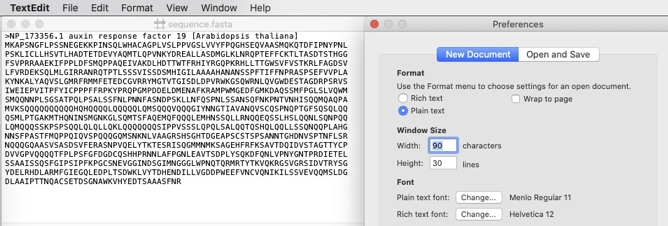
\includegraphics[width=1\linewidth]{files/textedit-0cc959f5c3e7cca8c6a83748cdd24856.png}
\caption[]{A screenshot of TextEdit on Mac.
Credits: \href{https://creativecommons.org/licenses/by-nc/4.0/}{CC BY-NC 4.0} \cite{own_1_2024}.}
\label{textedit}
\end{figure}

\begin{framed}
\textbf{See also}\\
If you are not yet familiar with plain text editors, then try it now and write and save a plain text file on your computer!
\end{framed}

There are some important file formats in bioinformatics.
A \textbf{fasta file} stores a DNA or protein sequence (Figure~\ref{fasta}).
Information on the sequence is found in the header (starting with \texttt{\textgreater }), which is on one line and the sequence can go over multiple lines.
A multi-fasta file stores multiple sequences.

\begin{figure}[!htbp]
\centering
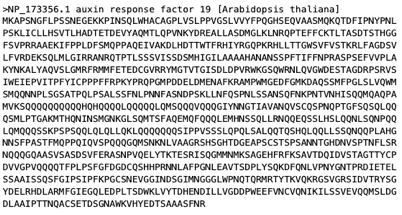
\includegraphics[width=0.5\linewidth]{files/fasta-838a5085fa938c75bc15fa75c6541b53.png}
\caption[]{A sequence in fasta format.
Credits: \href{https://creativecommons.org/licenses/by-nc/4.0/}{CC BY-NC 4.0} \cite{own_1_2024}.}
\label{fasta}
\end{figure}

The \textbf{GenBank file format} is a popular format to represent genes or genomes.
\href{https://www.ncbi.nlm.nih.gov/Sitemap/samplerecord.html}{Here} you can find an example GenBank record with annotations.
Important elements are the Locus, Definition (i.e., the name), and the Organism.
Additionally, Features, such as genes and CDSs (coding sequences) are listed.

\subparagraph{Binary files}

Binary files are all the files that are not text files, they cannot be opened in a text editor.
Instead, they need special programs to write and to open and interpret them.
Examples are word files (\texttt{.docx}) which can be opened with Word, pdf files (\texttt{.pdf}) which can be opened with Acrobat Reader, or image files (e.g., \texttt{.png}) which can be opened with image viewers.

Binary files are are also sometimes used in bioinformatics.
Examples include the bam format, which is a binary version of the sam format or the gzip format.
Gzip is used for compressing text files without the loss of information.
For large files, lots of disk space can be saved this way.


\bigskip
\centerline{\rule{13cm}{0.4pt}}
\bigskip

\subsubsection{Ontologies}\label{chapter1_ontologies}

An ontology is a comprehensive and structured vocabulary for a particular domain, such as biology, genetics, or medicine.
It defines the various terms used in a domain, along with their meanings and interconnections.
As such, ontologies serve as standardized frameworks for organizing and categorizing information in a way that enables effective communication and reasoning among researchers, practitioners, and computer systems.
For example, the terms in an ontology can encompass biological entities like genes, proteins, and cells, as well as processes, functions, and interactions that occur within living organisms.
Most of the databases mentioned mentioned in this chapter use ontologies in some way to describe their data.

Ontologies play a crucial role in bioinformatics because they facilitate:

\begin{enumerate}
\item \textbf{Standardization and consistency}: ontologies provide a common language and consistent framework for researchers and professionals, ensuring that everyone understands and uses terms in the same way.
\item \textbf{Interoperability}: ontologies facilitate the sharing and integration of data and knowledge across different research groups, institutions, and databases.
They enable computer systems to process data more accurately, leading to more meaningful analyses and discoveries.
\item \textbf{Scientific reasoning}: by organizing information in a logical and structured way, ontologies help researchers generate hypotheses, design experiments, and validate findings more effectively.
\end{enumerate}

\begin{framed}
\textbf{Note 1.9: FAIR principles}\\
As described above, ontologies facilitate scientific reproducibility.
A key concept in scientific reproducibility are the FAIR principles, with FAIR standing for Findable, Accessible, Interoperable, and Reusable.
This reader does not describe them in detail, but you should read the following online resource to familiarize yourself with the \href{https://www.go-fair.org/fair-principles/}{FAIR principles}.
\end{framed}

Ontologies typically form a hierarchy, where specific terms point to more generic terms. More generally, most ontologies are represented as a graph, where ontology terms are the nodes and relationships between terms are edges. As such, one ontology term may have more than one parent term.

A variety of ontologies are frequently used in the life sciences, some of which are discussed in greater detail below.

\paragraph{Gene Ontology}\label{chapter1_gene_ontology}

The \href{http://geneontology.org/}{Gene Ontology} (GO) is a knowledgebase for the function of genes and gene products (e.g. proteins). It is organised into three different domains covering various aspects:

\begin{itemize}
\item Molecular Function: molecular-level functions performed by gene products (e.g. proteins), such as `catalysis' or `transport'.
Most molecular functions can be performed by individual gene products, but some functions are performed by complexes consisting of multiple (possibly differing) gene products.
GO molecular functions often include the word ``activity'' (an \textit{amylase} enzyme would have the GO molecular function \textit{amylase activity}).
\item Cellular Component: the cellular structures (or location relative to them) in which a gene product performs its function.
Can be cellular compartments (e.g., \href{http://amigo.geneontology.org/amigo/term/GO:0005739}{mitochondrion}) or macromolecular complexes of which they are part (e.g., the \href{http://amigo.geneontology.org/amigo/term/GO:0005840}{ribosome}).
\item Biological Process: the larger biological programs composed of multiple molecular activities, for example \href{http://amigo.geneontology.org/amigo/term/GO:0006281}{DNA repair} or \href{http://amigo.geneontology.org/amigo/term/GO:0007165}{signal transduction}.
\end{itemize}

\begin{framed}
\textbf{Note 1.10: Molecular pathway?}\\
A biological process is not equivalent to a molecular pathway.
At present, the gene ontology does not represent the dynamics or dependencies that would be required to fully describe a pathway.
\end{framed}

A good example of how ontologies are represented as graphs is the biological process \href{http://amigo.geneontology.org/amigo/term/GO:0019319}{hexose biosynthetic process}, which has two parents: \href{http://amigo.geneontology.org/amigo/term/GO:0019318}{hexose metabolic process} and \href{http://amigo.geneontology.org/amigo/term/GO:0046364}{monosaccharide biosynthetic process}.
This reflects that biosynthetic process is a subtype of metabolic process and a hexose is a subtype of monosaccharide. (Figure~\ref{go}).

Edges between GO terms in the GO hierarchy can represent various relationships between genes and gene products.
The four main relationship types used in the gene ontology are `is a', `part of', `has part', and `regulates' (see Figure~\ref{so}).

\begin{figure}[!htbp]
\centering
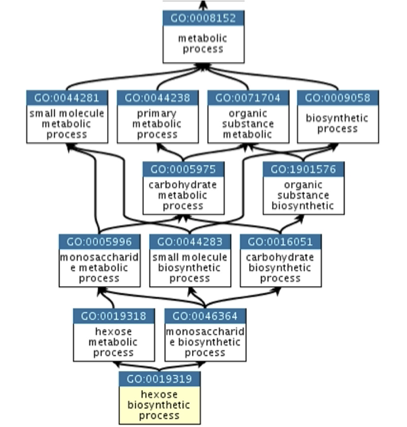
\includegraphics[width=0.55\linewidth]{files/go-67ecfd572d47f6ed3bdc35c0013264b8.png}
\caption[]{An extract of the Gene Ontology hierarchy.
Credits: \cite{go_2009}}
\label{go}
\end{figure}

\paragraph{Sequence Ontology}\label{chapter1_sequence_ontology}

The \href{http://sequenceontology.org}{Sequence Ontology} (SO) describes biological sequence elements such as genes or repeats, along with their features and attributes.

The sequence ontology is organized on four main levels:

\begin{itemize}
\item Attribute: an attribute describes a certain quality of a given sequence, for example the sequence source (i.e., how it was generated).
\item Collection: multiple discontiguous sequences together, for example the chromosomes of a complete genome.
\item Feature: the most general top-level entry that describes any extent of a continuous biological sequence, for example a \href{http://sequenceontology.org/browser/current\_release/term/SO:0000704}{gene} is a \href{http://sequenceontology.org/browser/current\_release/term/SO:0000001}{region}, which in turn is a sequence feature.
\item Variant: intended to describe genetic variation. The definition of a sequence variant is composed of other entries in the sequence ontology: ``A \href{http://sequenceontology.org/browser/current\_release/term/SO:0001060}{sequence\_variant} is a non-exact copy of a \href{http://sequenceontology.org/browser/current\_release/term/SO:0000110}{sequence\_feature} or \href{http://sequenceontology.org/browser/current\_release/term/SO:0001026}{genome} exhibiting one or more \href{http://sequenceontology.org/browser/current\_release/term/SO:0001059}{sequence\_alterations}''
\end{itemize}

\begin{figure}[!htbp]
\centering
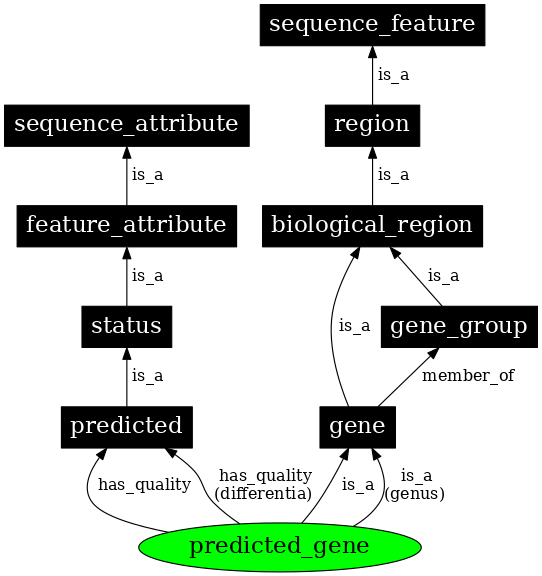
\includegraphics[width=0.4\linewidth]{files/sequence_ontology-3ebb78a944729d0afd7391447a463a9f.png}
\caption[]{An extract of the Sequence Ontology hierarchy.
Credits: \cite{so_2005}.}
\label{so}
\end{figure}

\paragraph{Other ontologies}\label{chapter1_other_ontologies}

Many more ontologies exist and are relevant to biomedical research.
The European Bioinformatics Institure (EBI) provides an \href{https://www.ebi.ac.uk/ols4/}{ontology lookup service} that facilitates searching for ontologies.
Examples of other ontologies are the \href{https://www.ebi.ac.uk/ols/ontologies/po}{plant ontology} that describes various anatomical structures in plants, and the \href{https://disease-ontology.org/}{human disease ontology}.


\bigskip
\centerline{\rule{13cm}{0.4pt}}
\bigskip

\subsubsection{Practical assignments}

This practical contains questions and exercises to help you process the study materials of Chapter 1.
You have 2 mornings to work your way through the exercises.
In a single session you should aim to get about halfway through this guide (i.e., day 1: assignment 1-3, day 2: assignment 4 and project preparation exercise).
Use the time indication to make sure that you do not get stuck in one assignment.
These practical exercises offer you the best preparation for the project.
Especially the \textbf{project preparation exercise} at the end is a good reflection of the level that is required to write a good project report.
Make sure that you develop your practical skills now, in order to apply them during the project.

\textbf{Note, the answers will be made available after the practical!}

\begin{framed}
\textbf{\textbf{Project Preparation Exercise}}\\
We want to obtain insights into members of the ARF gene family in \textit{Arabidopsis thaliana}.
ARF5 (UniProt ID P93024) and IAA5 (UniProt ID P33078) are two well-studied \textit{A. thaliana} proteins that play a role in auxin-mediated regulation of gene expression.
They are therefore chosen here as the starting points for exploring the plant ARF gene family.
Perform a small background study on ARF5 and IAA5.
Explore the protein sequences, properties (e.g., length, composition, etc.), interaction partners, and functional regions of ARF5 and IAA5.
Finally, explore the genes encoding ARF5 and IAA5 in \textit{A. thaliana} (genomic location, exon structure, expression, etc.).

Describe the following items in a few bullet points each.
You may include up to two figures or tables.

\begin{enumerate}
\item \textbf{Materials \& Methods} What did you do? Which data, databases and tools did you use, and why did you choose these? What important settings did you select?
\item \textbf{Results} What did you find, what are the main results? Report the relevant data, numbers, tables/figures, and clearly describe your observations.
\item \textbf{Discussion \& Conclusion} Do the results make sense? Are they according to your expectation or do you see something surprising? What do the results mean, how can you interpret them? Do different tools agree or not? What can you conclude? Make sure to describe the expectations and assumptions underlying your interpretation.
\end{enumerate}
\end{framed}

\subsubsection{Glossary}

\section{2. Alignment, sequence search, and primer design}

\begin{framed}
\textbf{Learning outcomes}\\
In this chapter, you will study sequence alignment.

Make sure you understand what DNA and protein alignments are used for and that you can explain the differences between local and global alignments.
You should be familiar with concepts related to alignments and sequence search, like dotplots, alignment scores, e-values, and substitution matrices.
Make sure you understand what multiple alignments are used for and that you can explain the differences between different solutions for the MSA problem.
You should understand what motifs are and the basics of profile hidden Markov models.
This chapter concludes with a section on PCR primer design as an example on the use of sequence alignment algorithms in practice.

During the practical you will learn how to make pairwise and multiple-sequence alignments, perform sequence searches and motif analyses, design primers, and discuss the results.
\end{framed}

\subsection{Introduction}

% #%[TODO: There can be more biological examples in this section]

Comparing DNA and protein sequences is a key tool in the field of applied bioinformatics.
By analyzing these sequences, researchers can annotate genes from new genomes, build models of protein structures, and investigate gene expression, i.e., which genes are turned on and off.
It is important to notice that nature tends to stick with what works, rather than reinventing the wheel for each species.
Instead, organisms evolve from ancestors, they accumulate mutations (Chapter~1), and gradually develop new traits over time.
That means that similar genes can be found in different organisms and the functional information can be transferred from one protein to another if both possess a certain degree of similarity.
However, even though two proteins may look similar, they could also have different functions.
Generally, similarities arise because of shared ancestry (divergent evolution), nevertheless, similarities can also appear independently (convergent evolution).

Before diving into the analysis of whether sequences are related, it is important to understand some key terms.

\begin{framed}
\textbf{Homology and similarity}\\
\textbf{Homology} means that sequences share a common evolutionary history and therefore have a common ancestor.
Homology is not quantifiable.
If two sequences have a common ancestor, they are homologous.
Thus, two sequences are either homologous or they are not.

\textbf{Sequence identity} and \textbf{sequence similarity} are often used to infer whether two sequences are homologous.
We can measure the identity or similarity between sequences and we will see how to do this later in this chapter.

In contrast, we cannot measure homology, but we can only infer it.
\end{framed}

\begin{framed}
\textbf{See also}\\
Here is a classic paper on homologous protein families: \href{https://pubmed.ncbi.nlm.nih.gov/9381173/}{Tatusov et al., 1997}.
\end{framed}

\subsection{Dot plots}

Dot plots are a simple way to visualize similar regions between two sequences.
They are represented by a two-dimensional array, where one sequence is written vertically and the other horizontally.
A dot is placed in a cell, where the residues are identical.
In the resulting plot, similar regions appear as diagonal stretches and insertions and deletions appear as a discontinuity in a diagonal line (Figure~\ref{dotsmall}).

\begin{figure}[!htbp]
\centering
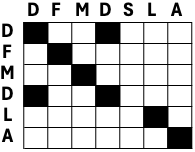
\includegraphics[width=0.9\linewidth]{files/dot_small2-db4f4d0b90fecfbd44f5897dc049fa70.png}
\caption[]{A small example of a dotplot. \newline
Credits: \href{https://creativecommons.org/licenses/by-nc/4.0/}{CC BY-NC 4.0} \cite{own_2_2024}.}
\label{dotsmall}
\end{figure}

A sequence can also be compared to itself, then the main diagonal will be filled with dots and additional repeats are on the off-diagonal (Figure~\ref{dotlarge}).

\begin{figure}[!htbp]
\centering
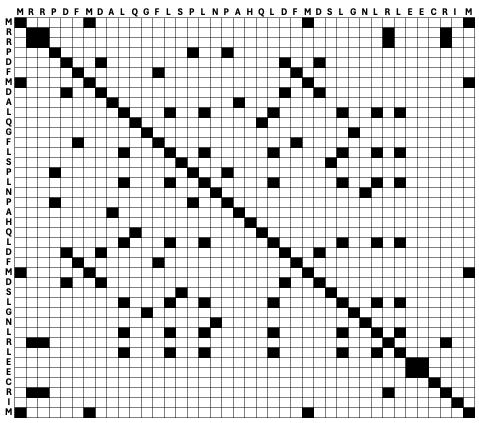
\includegraphics[width=1\linewidth]{files/dot_large-dc5236a779ddd7ca60530ad37c9d5291.png}
\caption[]{An example of a dotplot to compare a sequence with itself. Credits: \href{https://creativecommons.org/licenses/by-nc/4.0/}{CC BY-NC 4.0} \cite{own_2_2024}.}
\label{dotlarge}
\end{figure}

This simple way of marking identical residues shows a lot of background noise.
To detect interesting patterns, typically a filter is applied.
For example, a minimum identity should be present across a certain window size, i.e., consecutive number of residues being considered.
This feature is implemented in a webserver to visualize dotplots, \href{https://dotlet.vital-it.ch/}{dotlet} \cite{dotlet_2000} (Figure~\ref{dotweb}).

\begin{figure}[!htbp]
\centering
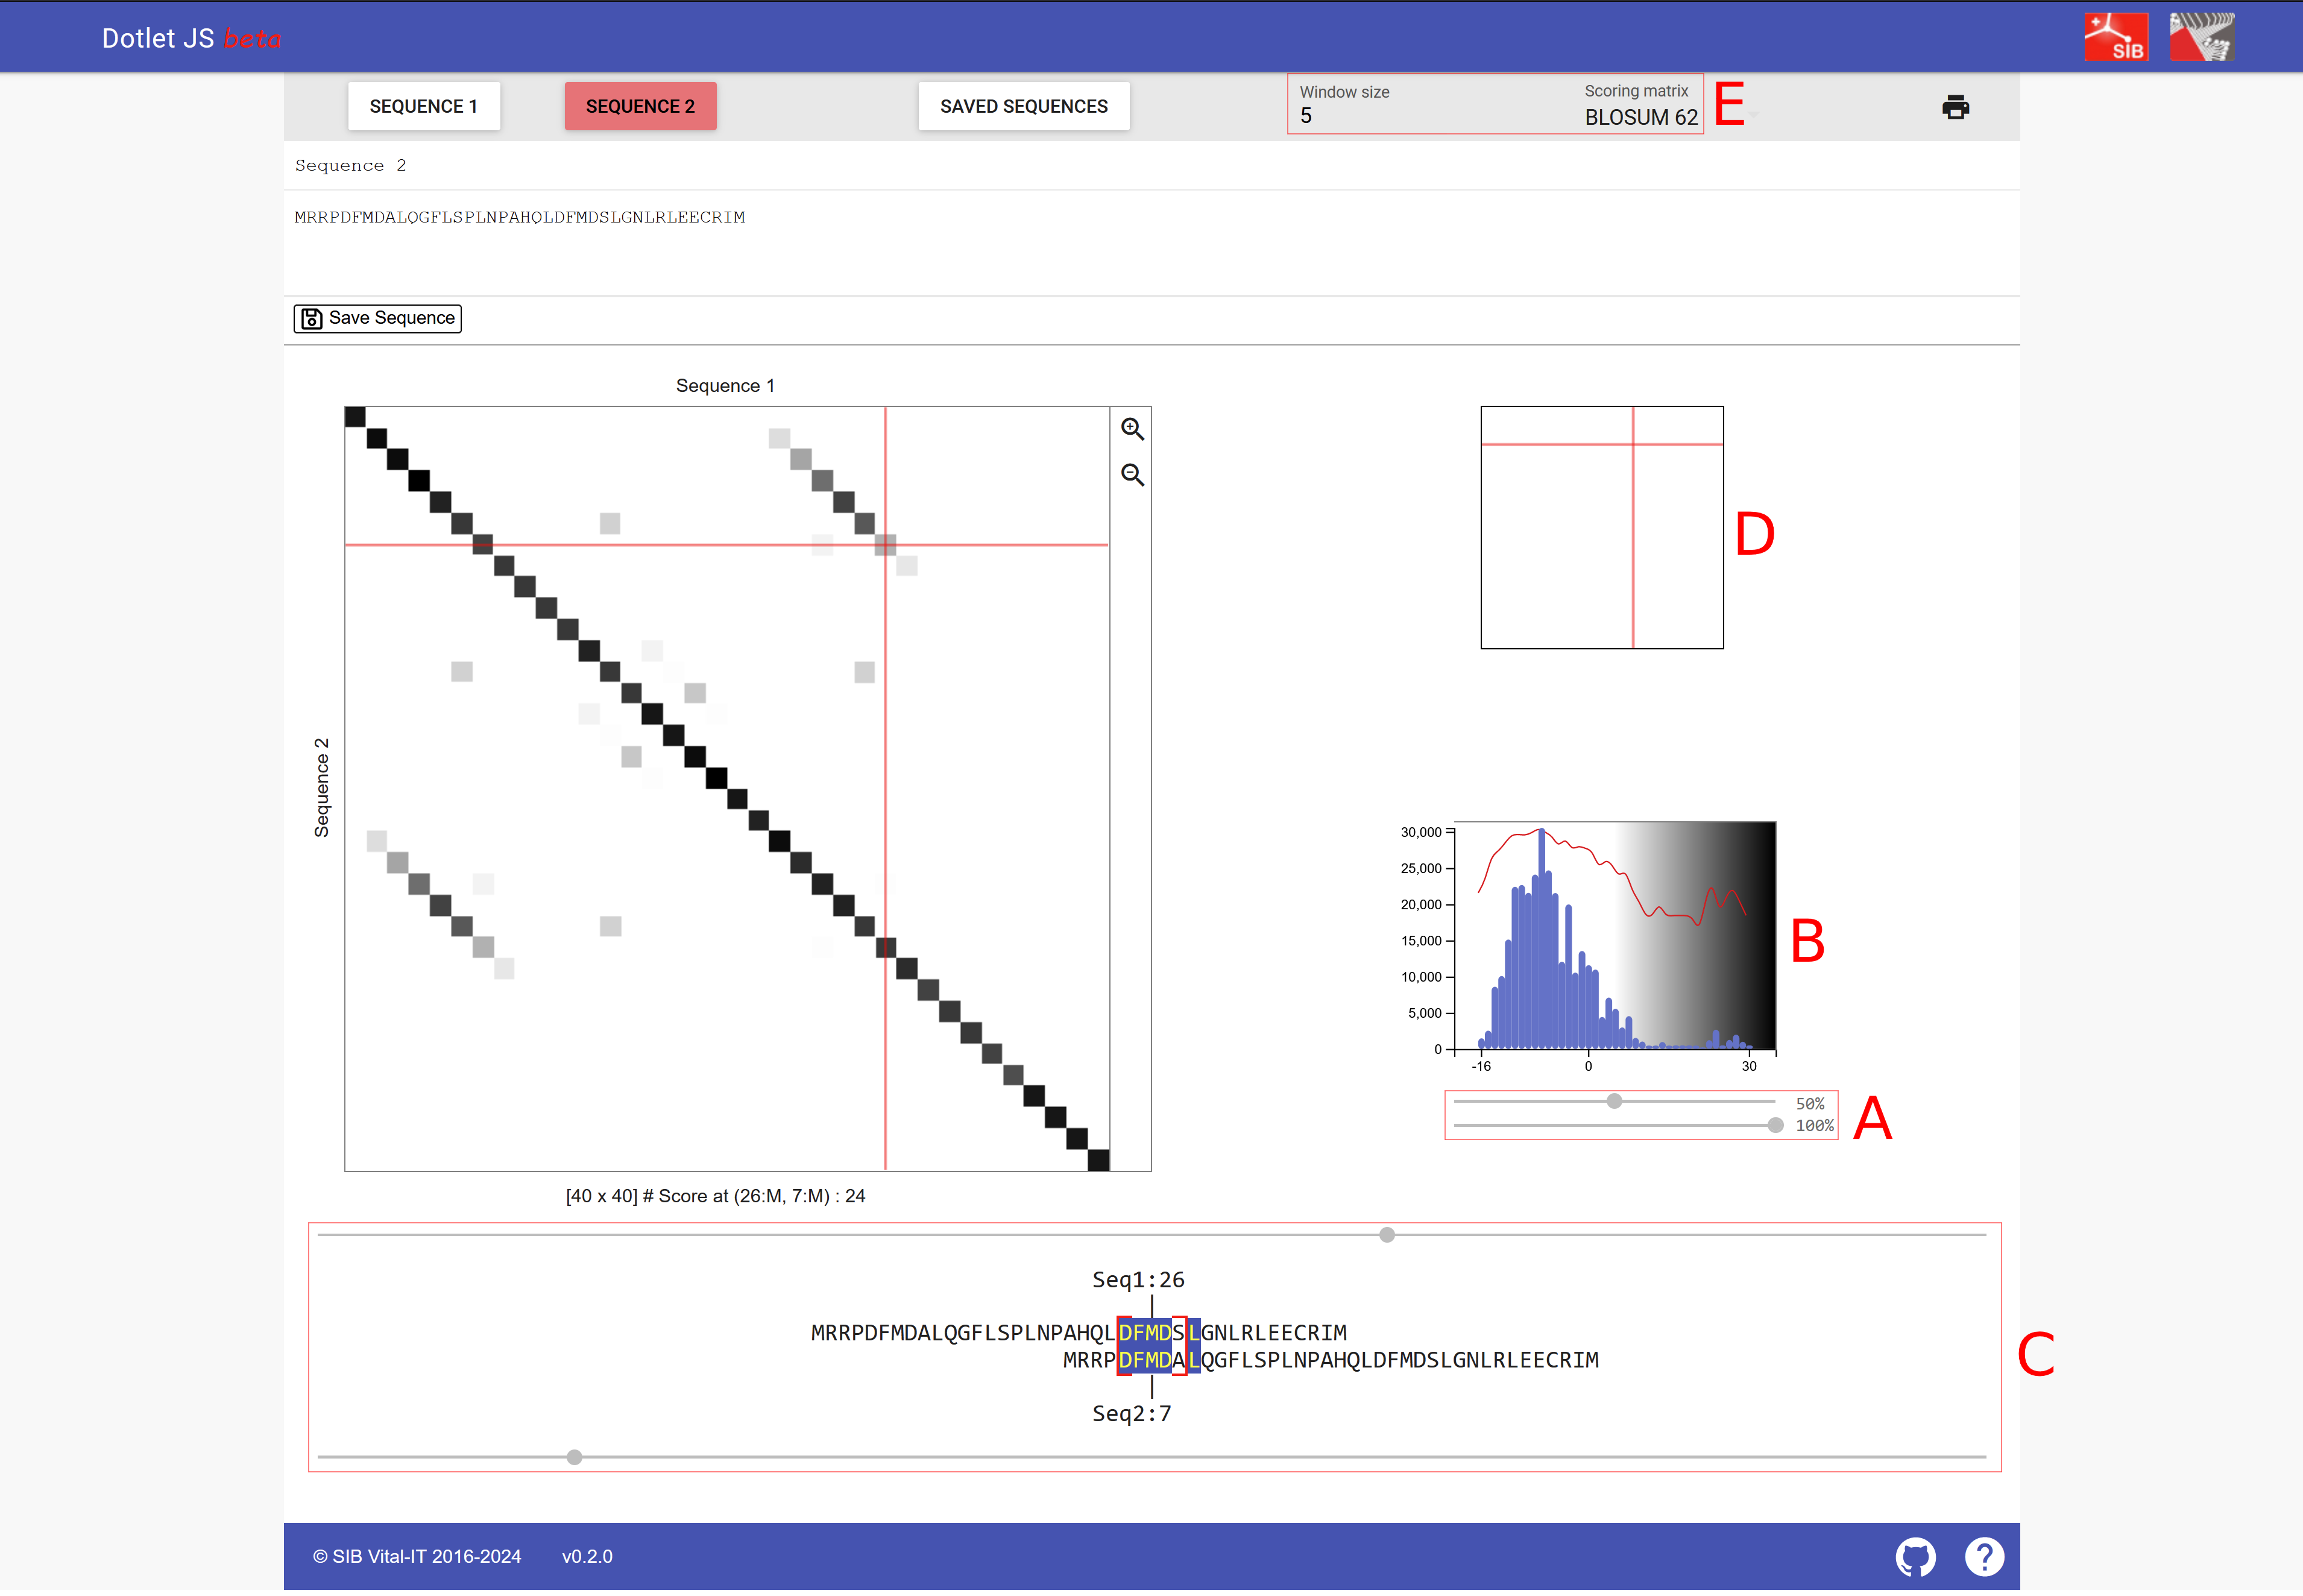
\includegraphics[width=1\linewidth]{files/dot_web-0662600de881673d53ee7891b616612c.png}
\caption[]{A screenshot of \href{https://dotlet.vital-it.ch/}{dotlet} with sequence \texttt{MRRPDFMDALQGFLSPLNPAHQLDFMDSLGNLRLEECRIM}.

\begin{itemize}
\item (A) The two sliders to change the appearence of the plot: The top slider can adjust the sensitivity, moving it to the right, fewer similar regions are shown; moving it to the left, also regions with lower similarity appear.
The bottom slider adjusts the color scheme and is less relevant compared to the top slider.
\item (B) The histogram indicates how many hits with a particular similarity are shown; thus the slider can be adjusted to the right tail of the histogram.
\item (C) The two sliders that can adjust how the two sequences are positioned against each other.
\item (D) Serves a similar function as the two sliders of C but allows for arrow key navigation of the dotplot.
\item (E) Here you can select the window size of sequence comparison and the scoring matrix (window size is explained below and substitution matrices will also be explained below).
\item Credits: \cite{dotlet_2000}.
\end{itemize}}
\label{dotweb}
\end{figure}

\subsection{Pairwise alignment}

Dot plots provide a visual way to compare two sequences, however, they do not provide the similarity between two sequences.
To calculate sequence similarity or sequence identity, we need to perform a \textbf{pairwise sequence alignment}.
In an alignment, the two sequences will be placed above each other and gaps can be introduced to represent insertions or deletions of residues.
We also say that the two sequences will be \textbf{aligned}.
The resulting alignment contains matches, mismatches, and gaps (Figure~\ref{algterm})

\begin{figure}[!htbp]
\centering
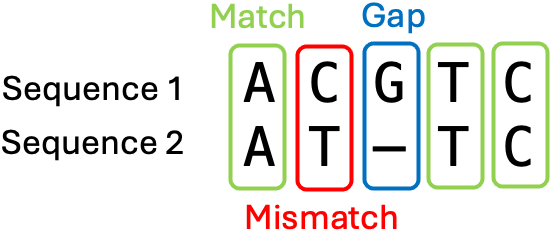
\includegraphics[width=0.5\linewidth]{files/alg_term-f276ccefbf1d202caaf7f23d7464dc58.png}
\caption[]{A small example of two aligned sequences.
Credits: \href{https://creativecommons.org/licenses/by-nc/4.0/}{CC BY-NC 4.0} \cite{own_2_2024}.}
\label{algterm}
\end{figure}

\subsubsection{Alignments of DNA sequences}

Every position in a sequence could potentially have an instertion or a deletion, so there are many possible locations and combinations for gaps and thus many potential alignments.
The final alignment will be the one with the maximum total alignment score.
This score is determined by the scoring parameters that are chosen before the alignment calculation.
An example of DNA sequence scoring paramaters could be that matches score 1 and mismatches -1 and that there is a gap penalty of -1.
The total alignment score is calculated by summing over all columns in the alignment (Figure~\ref{algscore}).

\begin{figure}[!htbp]
\centering
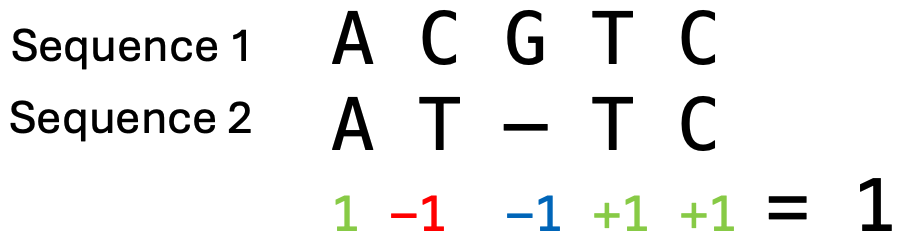
\includegraphics[width=0.6\linewidth]{files/alg_score-2bc8cb8229af1c45cf35062f015e5541.png}
\caption[]{An example calculation of the alignment score, where matches score 1, mismatches -1 and there is a gap penalty of -1.
This results in a total score of 1 for this alignment.
Credits: \href{https://creativecommons.org/licenses/by-nc/4.0/}{CC BY-NC 4.0} \cite{own_2_2024}.}
\label{algscore}
\end{figure}

The choice of the scoring parameters has an impact which alignment will have the maximum score.
To understand the impact of the parameters on the final alignment, fill in table Figure~\ref{algex}.

\begin{figure}[!htbp]
\centering
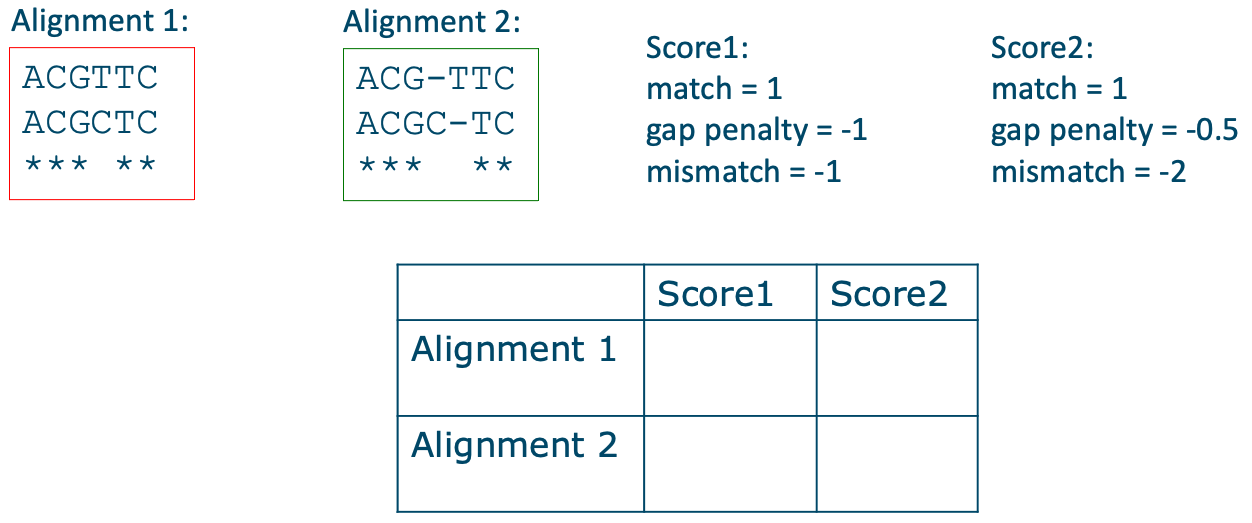
\includegraphics[width=1\linewidth]{files/alg_exercise-44d2e5d97743e3370181c88ae34956bf.png}
\caption[]{\textbf{Assignment}: Fill the table for the two alignments and the two sets of scoring parameters.
Credits: \href{https://creativecommons.org/licenses/by-nc/4.0/}{CC BY-NC 4.0} \cite{own_2_2024}.}
\label{algex}
\end{figure}

\begin{framed}
\textbf{Note 2.1: Affine gap costs}\\
The DNA and protein sequences that we want to align often have varying lengths, which is the result of insertions and deletions during evolution.
Insertion and deletion events can affect one or multiple residues, where one event of length 2 is more likely to happen than two independent events of length 1.
To include this in the scoring scheme, alignment programms use \textbf{affine gap costs} that distinguish between opening a gap and extending a gap.
For example, the default parameters of the pairwise alignment program \href{https://www.ebi.ac.uk/jdispatcher/psa/emboss\_needle}{needle} \cite{EMBL_tools_2022} are:

Gap open (score for the first residue in a gap): -10

Gap extend (score for each additional residue in a gap): -0.5
\end{framed}

\subsubsection{Alignments of protein sequences}

\paragraph{Substitution matrices}\label{chapter2_substitution_matrices}

In chapter~1, we learned that different amino acids have different chemical properties.
When the protein structure and function are conserved, it is more likely that an amino acid gets exchanged by a chemically similar amino acid, compared to a very different one.
When aligning protein sequences, we thus want to penalize the exchange of chemically dissimilar amino acids and reward the exchange of chemically similar amino acids.
To this end, the score of matches and mismatches is generally determined by a \textbf{substitution matrix}, e.g., BLOSUM62 - \textbf{BLOSUM (BLOck SUbstitution Matrix)} (Figure~\ref{blosum62}).
The substitution matrix and the gap parameters then determine the alignment score (Figure~\ref{aa_alg}).

\begin{figure}[!htbp]
\centering
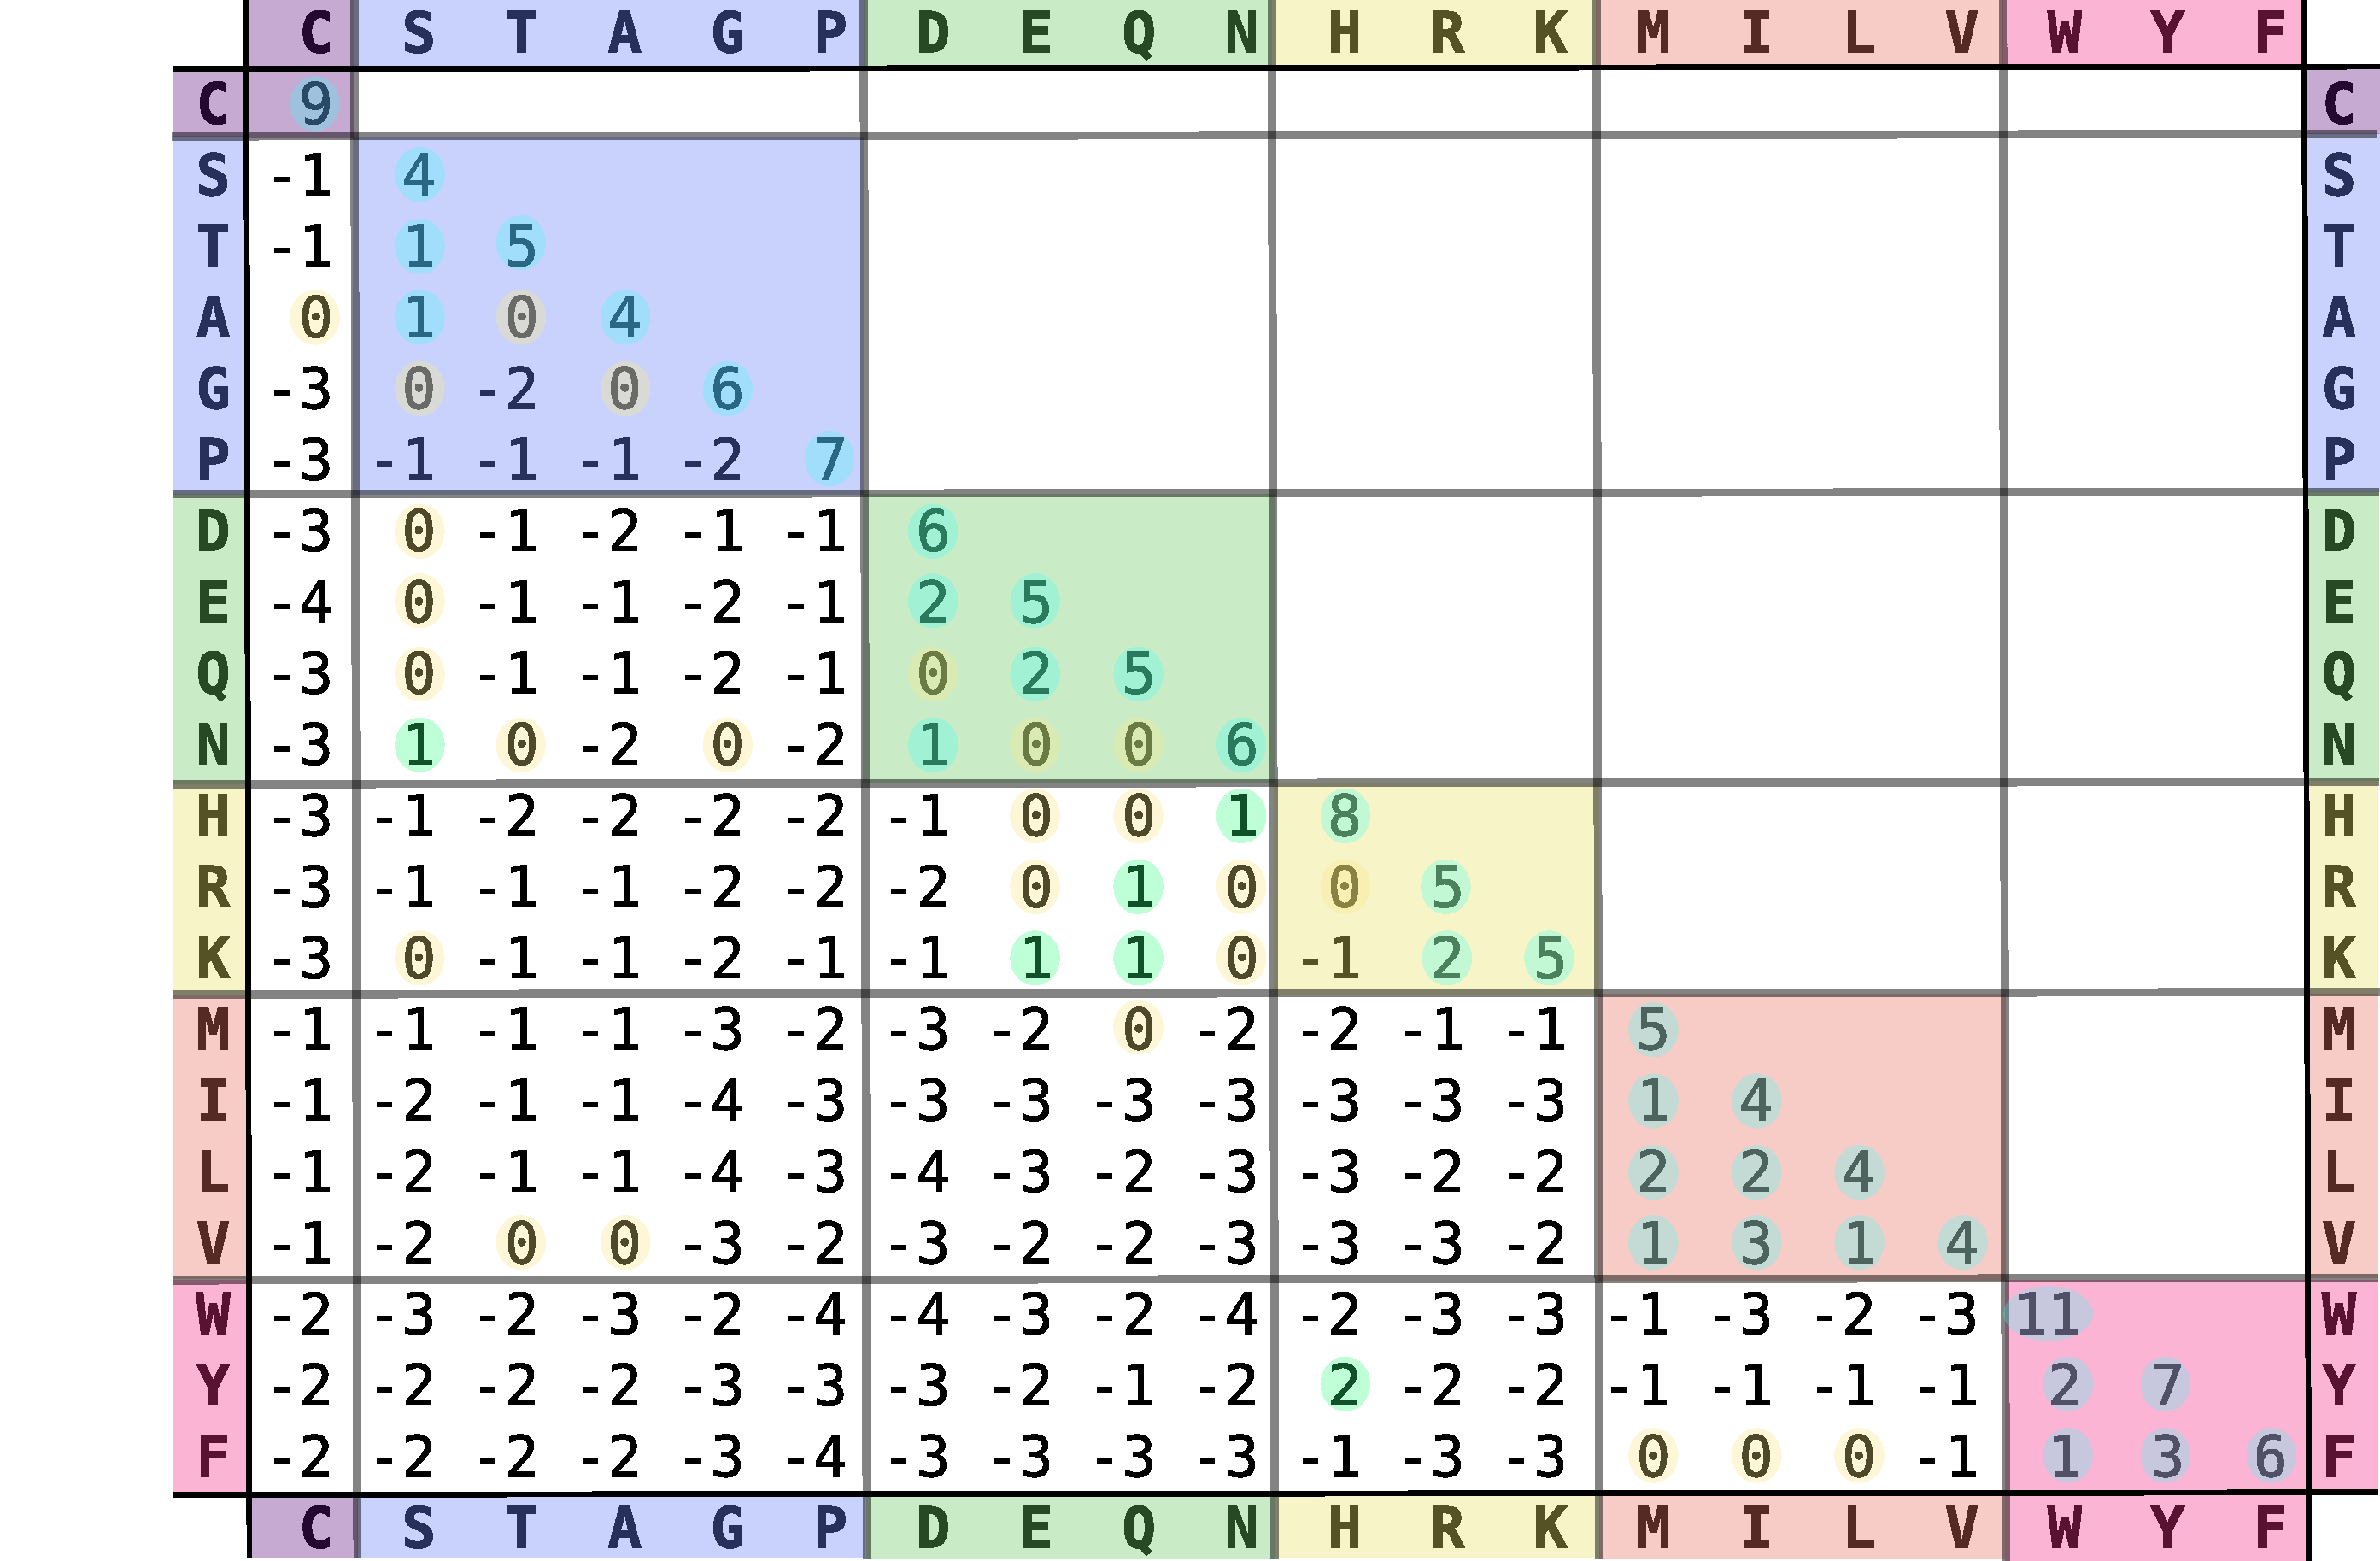
\includegraphics[width=1\linewidth]{files/blosum62-998aa3486f71a507d639852ff7479e95.pdf}
\caption[]{The BLOSUM62 amino acid substitution matrix.
The matrix is ordered and positive values and zero values are highlighted.
Credits: \href{https://creativecommons.org/licenses/by-sa/4.0/}{CC BY-SA 4.0} \cite{blosum62_2022}.}
\label{blosum62}
\end{figure}

\begin{framed}
\textbf{Box 2.1: Assignment}\\
Look at the amino acid properties in the table in chapter~1, choose some amino acids with the same properties and some with different properties.
Then look up these pairs in the BLOSUM62 matrix.
What do you observe?
\end{framed}

\begin{figure}[!htbp]
\centering
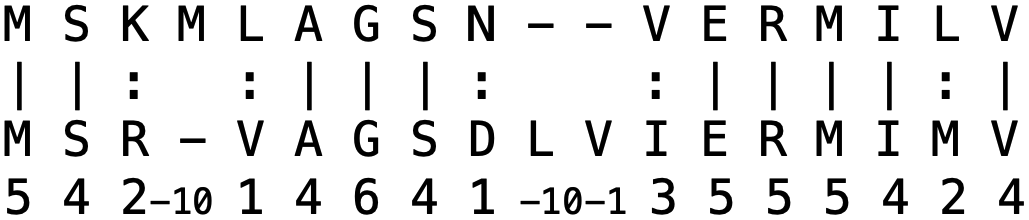
\includegraphics[width=1\linewidth]{files/aa_alg-cf3f1a5e13f7346c86c1b95980331ff4.png}
\caption[]{Example of a pairwise protein alignment.
With the BLOSUM62 scoring matrix, a gap opening score of -10, and a gap extension score of -1, the resulting alignment score is 34.
Credits: \href{https://creativecommons.org/licenses/by-nc/4.0/}{CC BY-NC 4.0} \cite{own_2_2024}.}
\label{aa_alg}
\end{figure}

Note that we motivated the use of amino acid substitution matrices by the chemical properties of amino acids; however, these properties were not directly used when determining these matrices.
Instead, the BLOSUM matrix is determined by aligning conserved regions from Swiss-Prot (chapter~1) and clustering them based on identity.
Then, the substitutions between the different pairs of amino acids within a cluster are counted, which is used to compute the BLOSUM scores.
Thus, these scores reflect directly which amino acids are exchanged more often with each other over evolutionary time and we can observe that this frequency is strongly correlated to their chemical properties.
There are different versions of BLOSUM, for example BLOSUM62 was derived by clustering sequences with an identity of 62\% and it is appropriate for comparing protein sequences having around 62\% identity.
Other available matrices are for example BLOSUM45 and BLOSUM80 (Figure~\ref{submat}).

Another group of matrices that was derived even before BLOSUM is \textbf{PAM (Point Accepted Mutation)}.
The entries in a PAM matrix denote the substitution probabilities of amino acids over a defined unit of evolutionary change.
For example, PAM1 represents one substitution per 100 amino acid residues and is thus appropriate for very closely related sequences.
A commonly used matrix is PAM250, which means that 250 mutations happened over 100 residues; that is, many residues have been affected by more than one mutation.

\begin{figure}[!htbp]
\centering
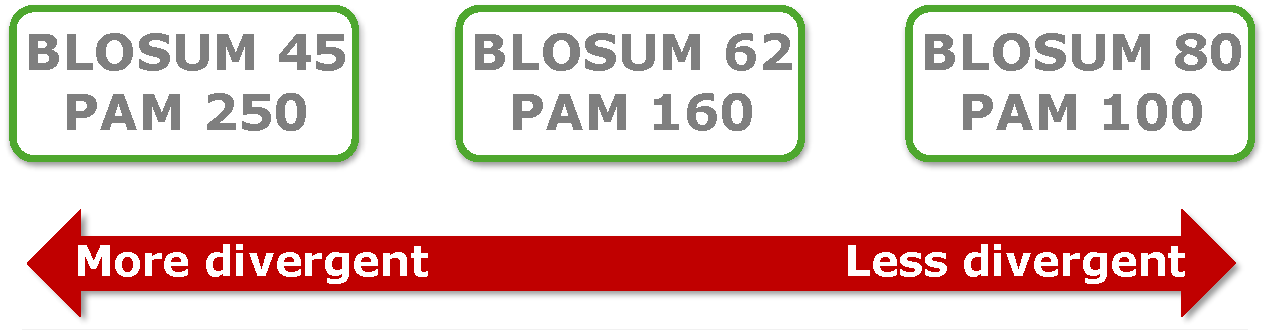
\includegraphics[width=0.8\linewidth]{files/submat-50e39b907c3803a8ca0b3f7fe7f14a07.pdf}
\caption[]{An overview of different available substitution matrices.
Credits: \href{https://creativecommons.org/licenses/by-nc/4.0/}{CC BY-NC 4.0} \cite{own_2_2024}.}
\label{submat}
\end{figure}

\begin{framed}
\textbf{See Also}\\
An introduction into PAM and BLOSUM substitution matrices.
\end{framed}

\paragraph{Protein identity and similarity}

For two protein sequences, we can distinguish two different measures of how much they are alike: identity and similarity, which are defined slightly differently.
The \textbf{protein identity} is given by the number of identical amino acids divided by the alignment length.
The \textbf{protein similarity} is given by the number of similar amino acids \textbf{and} the number of identical amino acids divided by the alignment length.
In the pairwise alignment program \href{https://www.ebi.ac.uk/jdispatcher/psa/emboss\_needle}{needle}, \textbf{identical amino acids} are marked by a pipe symbol/vertical line (|), \textbf{similar amino acids} are marked by a colon (:) and defined by pairs that have a positive score (i.e., \textgreater 0) in the chosen substitution matrix (Figure~\ref{aa_sim}).

\begin{figure}[!htbp]
\centering
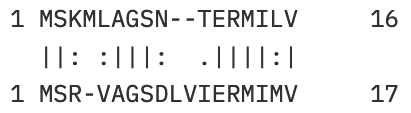
\includegraphics[width=0.6\linewidth]{files/aa_sim-813512ae657cda606e163020688689f4.png}
\caption[]{Example protein alignment. The percent identity is 10 / 18 = 55.6\% and the percent similarity is 14 / 18 = 77.8\%.
Credits: \href{https://creativecommons.org/licenses/by-nc/4.0/}{CC BY-NC 4.0} \cite{own_2_2024}.}
\label{aa_sim}
\end{figure}

Note that the pairwise alignment method does not try to maximize similarity or identity, but they are a result of the chosen parameters.
Especially for distantly related sequences, the parameters can have a big impact on the alignment and thus on the estimated identity and similarity.
In Figure~\ref{alg_gap}, you can find an example of two protein kinases from rice.

\begin{figure}[!htbp]
\centering
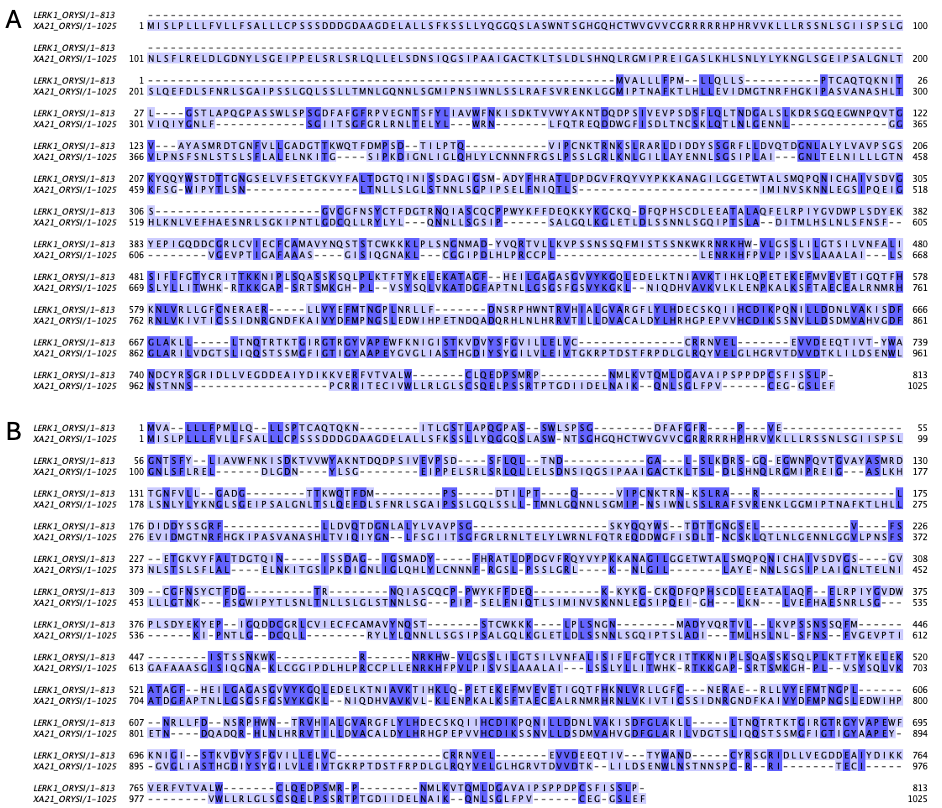
\includegraphics[width=1\linewidth]{files/alg_gap-a25ce3110d8094cc1b4da311bca7e507.png}
\caption[]{Alignments of the same two sequences (LERK1\_ORYSI and XA21\_ORYSI) with different parameters:
A) BLOSUM62 matrix, gap open: -10, gap extend: -0.5. Identity = 210/1191 (17.6\%), Similarity = 345/1191 (29.0\%).
B) BLOSUM62 matrix, gap open: -5, gap extend: -0.5. Identity = 305/1166 (26.2\%), Similarity = 428/1166 (36.7\%).
Credits: \href{https://creativecommons.org/licenses/by-nc/4.0/}{CC BY-NC 4.0} \cite{own_2_2024} made using \href{https://www.ebi.ac.uk/jdispatcher/psa/emboss\_needle}{needle} \cite{EMBL_tools_2022}.}
\label{alg_gap}
\end{figure}

Up until now, we have only considered pairwise alignments, where both sequences are aligned completely, these are called \textbf{global alignments}.

\begin{framed}
\textbf{Note 2.2: Finding the best alignment}\\
There is a huge number of alignments possible for two sequences, since the gaps can be placed in many different ways.
However, to find the \textbf{optimal alignment}, i.e., the one with the highest score, it is not necessary to explore all these possibilities.
Efficient algorithms exist that guarantee to find the optimal alignment.
The Needleman-Wunsch algorithm was the first algorithm and can solve this task in a time that is quadratic to the length of the input sequences.
\end{framed}

\subsubsection{Local alignments}

The previous example shows that some sequences might not be related over their full length.
We have seen in chapter~1 that many proteins are composed of domains.
When comparing two proteins, only some parts that correspond to the domains might be related.
Then, it is more appropriate to perform a \textbf{local alignment}.
Local alignment is also a good tool for identifying functional sites from which sequence patterns and motifs can be derived Figure~\ref{alg_local}.

The aim of a local alignment is to find the best subsequences of both input sequences that result in the maximum alignment score given the alignment parameters.
As for global alignment, efficient algorithms exist to solve this task.
The Smith-Waterman algorithm can also solve this task in a time that is quadratic in the length of the input sequences, just like the Needleman-Wunsch algorithm for global alignments.

\begin{figure}[!htbp]
\centering
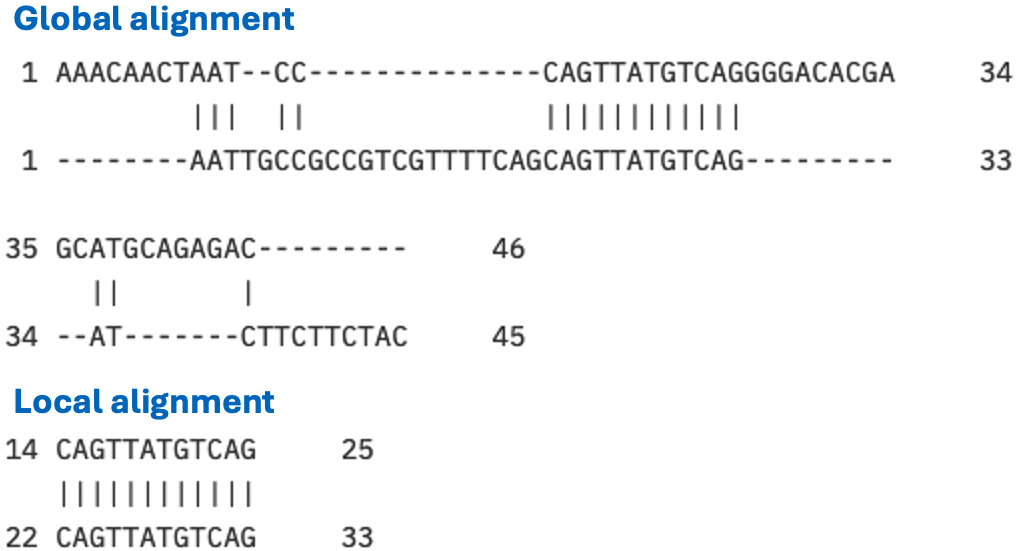
\includegraphics[width=1\linewidth]{files/alg_local-4f60831aa4af06a36d5d4c5a4124517f.png}
\caption[]{Alignments of the same two sequences, once using the global alignment program \href{https://www.ebi.ac.uk/jdispatcher/psa/emboss\_needle}{needle} and once using the local alignment program \href{https://www.ebi.ac.uk/jdispatcher/psa/emboss\_water}{water} \cite{EMBL_tools_2022}.
The same alignment paramters were used: \href{https://rosalind.info/glossary/dnafull/}{DNAfull matrix}, gap open -10, gap extend -0.5.
The global identity is 20/71 (28.2\%) and the local identity is 12/12 (100.0\%).
Credits: \href{https://creativecommons.org/licenses/by-nc/4.0/}{CC BY-NC 4.0} \cite{own_2_2024}.}
\label{alg_local}
\end{figure}

\subsection{Search in sequence databases}\label{chapter2_sequence_search}

In Chapter 1, we learned about different sequence~databases.
We often want to search novel sequences in these databases, for example to learn which other organisms have homologs.
Two sequences that are highly similar, might also share the same function.
This relationship is used for the functional~annotation of sequences, where the search in databases is an important step.

\begin{framed}
\textbf{Note 2.3: Similarity by chance}\\
When all nucleotides occur randomly and at the same frequency, then each sequence of length \texttt{x} is expected to occur with a frequency of 1/4\textsuperscript{x}, e.g., a sequence of length 3 has a frequency of 1/64 and a sequence of length 10 has a frequency of about 1 in a million.
This becomes important since these days, databases are very large, they can contain millions of sequences.
Due to this large amount of data, some similarities might just be observed by chance, especially if our sequence of interest is short.
Thus, statistical methods have been developed to estimate if an observed alignment might have just occured due to chance (see below).
\end{framed}

\subsubsection{Database search vs. pairwise alignment}

Pairwise alignments are also used when searching sequences in sequence databases.
In this task, we have a query sequence and we want to find similar sequences in a database; these similar sequences are called subjects or hits.
Although the algorithms that were discussed in the previous section are relatively fast when two sequences are aligned, it would still take too long overall to perform pairwise sequence alignments of the query with all potential subjects from the database.
We thus need even more efficient algorithms.

\begin{framed}
\textbf{Note 2.4: Heuristic algorithms}\\
The Needleman-Wunsch and the Smith-Waterman algorithm described in the previous section guarantee to find the alignment with the best score for the given sequences and parameters.
In contrast, an \textbf{heuristic algorithm} employs some heuristics, which generally lead to good results and which make the algorithm much faster. However, the method does not guarantee to find the optimal score anymore.
\end{framed}

\subsubsection{BLAST}

Basic Local Alignment Search Tool (\textbf{BLAST}) is a heuristic method to find regions of local similarity between protein or nucleotide sequences.
The program compares nucleotide or protein sequences to sequences in a database and calculates the statistical significance of the matches.
Both the standalone and web version of BLAST are available from the National Center for Biotechnology Information (\href{https://www.ncbi.nlm.nih.gov}{NCBI}).

\paragraph{The algorithm}\label{chapter2_blast_algorithm}

The starting point of BLAST is the set of words that two sequences have in common, where a word is a part of a sequence of a fixed length.
For protein blast, the default word size is 5 and for nucleotide blast it is 11.
To find these common words, first a lookup table of the query words is reconstructed (Figure~\ref{blast_figure}A), where neighborhood words are listed as well.
Neighborhood words are all the words that have a high alignment score with the query word (Figure~\ref{blast_figure}B).
Then, BLAST scans the database for word matches.
For protein blast, two matches within 40 residues must be found such that the BLAST considers the hit as an initial match (Figure~\ref{blast_figure}C).
Note that for nucleotides, initial hits are found in a simpler way:
Only one exact match must be found, i.e., no neighborhood is considered.

After finding initial matches, BLAST extends these matches into local alignments (Figure~\ref{blast_figure}D).
As this extension happens, the alignment score increases or decreases.
When the alignment score drops below a set level, the extension stops.
This prevents the alignment from stretching into areas where there is very little similarity between the query and hit sequences.
If the obtained alignment receives a score above a certain threshold, it will be included in the final BLAST result.
BLAST is thus a heuristic algorithm, but its careful process helps to ensure a reasonable trade-off between run time and accuracy.

\begin{figure}[!htbp]
\centering
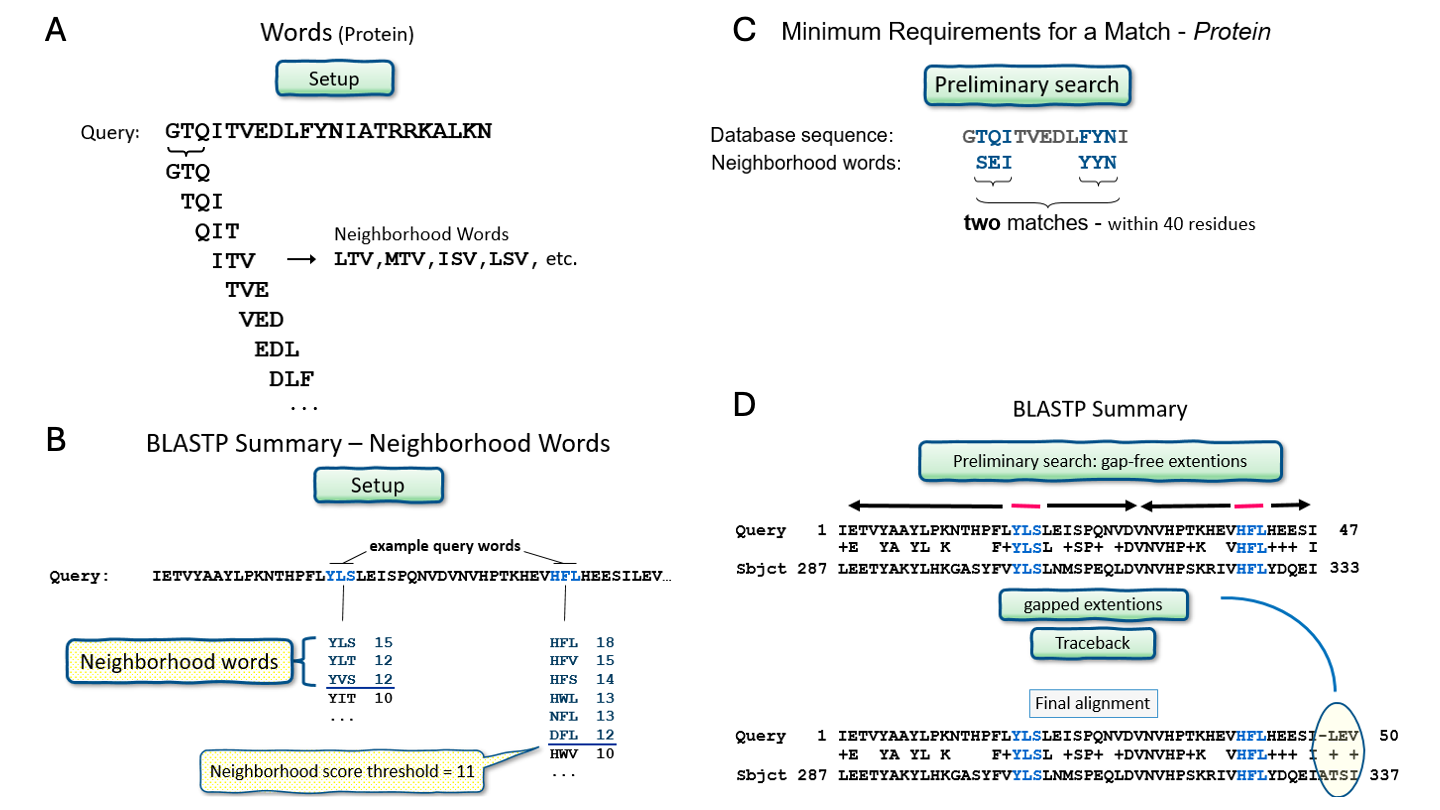
\includegraphics[width=1\linewidth]{files/blast-d0e05e10ecd313dcc8deac97dde44ba2.png}
\caption[]{An overview of the BLAST algorithm.
Credits: \href{https://creativecommons.org/publicdomain/zero/1.0/}{CC0 1.0} \cite{blast_2022}.}
\label{blast_figure}
\end{figure}

\paragraph{BLAST output}

The BLAST output contains vast information on the found hits, their alignments, and taxonomy (Figure~\ref{blast_output}).

\begin{figure}[!htbp]
\centering
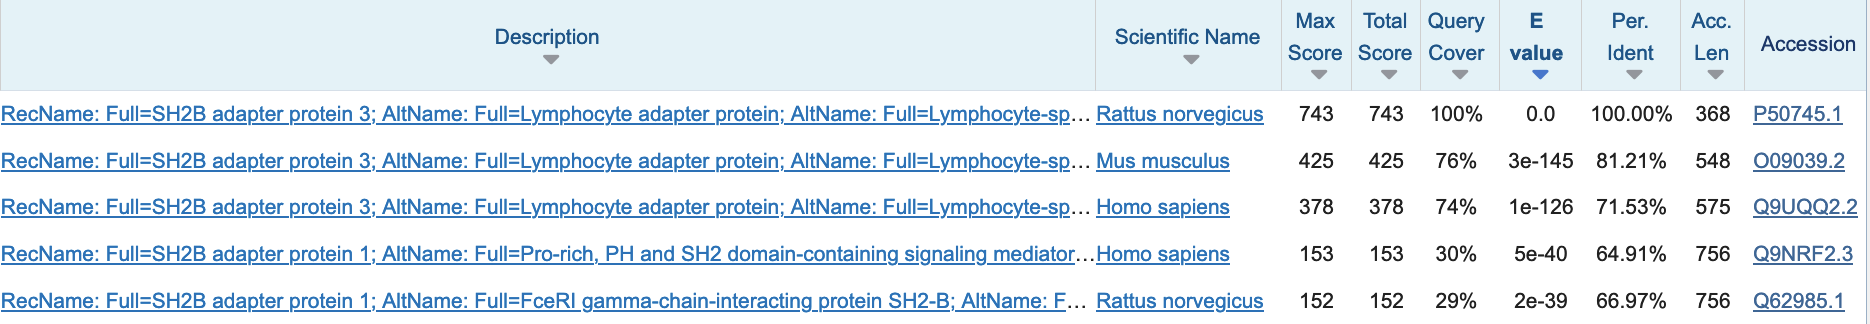
\includegraphics[width=1\linewidth]{files/blast_output-fb4ececca6ae3390731902ad57c4b880.png}
\caption[]{Top 5 blast hits when searching the rat protein P50745 in the Swiss-Prot 2024\_02 release database.
Credits: \cite{blast_2009}}
\label{blast_output}
\end{figure}

\begin{framed}
\textbf{Note 2.5: E-value}\\
An important output statistic is the expectation value (\textbf{e-value}), which is the number of BLAST hits you expect to see by chance in the database, with the observed score or higher.
Note that due to this definition, the e-value depends on the database size.
Since it is more likely to find something by chance in a larger database, the e-value for the same hit would be higher compared to a smaller database.
Thus, to find as many good hits as possible, it makes sense to use the smallest specific database that contains all the sequences you are interested in.
For example, if you are only interested in plants, then restrict your search to only plant sequences.
During the practical you will get to know how to do that in the online BLAST interface.

The BLAST output is sorted by increasing e-value.
This can result in very low numbers and the BLAST output uses the scientific notation to list these, where e.g., 3e-145 means 3*10\textsuperscript{-145}.
Thus, the hits listed in Figure~\ref{blast_output} are likely not random, since their number to be observed by chance is very low.
If the alignment is not by chance, then it might be due to a biological meaningful relationship between the two sequences.
However, it is difficult to define a clear e-value cutoff for biologically meaningful hits.
Commonly used cutoffs are 1e-5 or 1e-10.
\end{framed}

Note that you cannot infer homology by e-value alone, also the coverage and percent identity need to be taken into account.
For example, in Figure~\ref{blast_output}, all hits have very low e-value:
the first hit is to the sequence itself, then there are hits with high identity and high coverage in mouse and human, these might be homologous sequences.
The 4\textsuperscript{th} and 5\textsuperscript{th} hit are only local, since the query cover is {\textasciitilde}30\%, these sequences might only share a homologous domain with the query protein.

\paragraph{BLAST types}

Different types of BLAST exist to search nucleotides or proteins in the respective databases:
\texttt{blastn} searches a nucleotide sequence in a nucleotide database and \texttt{blastp} searches a protein sequence in a protein database.
In addition, the query and/or the database can also be translated in all six reading frames to allow additional kinds of comparisons (Figure~\ref{blast_types}).

% #%[TODO: check that the reading frame translation is clear from chapter 1 or explain more]

Different BLAST types exist for these different kinds of comparisons, where these translations are done automatically (Figure~\ref{blast_types}).

\begin{figure}[!htbp]
\centering
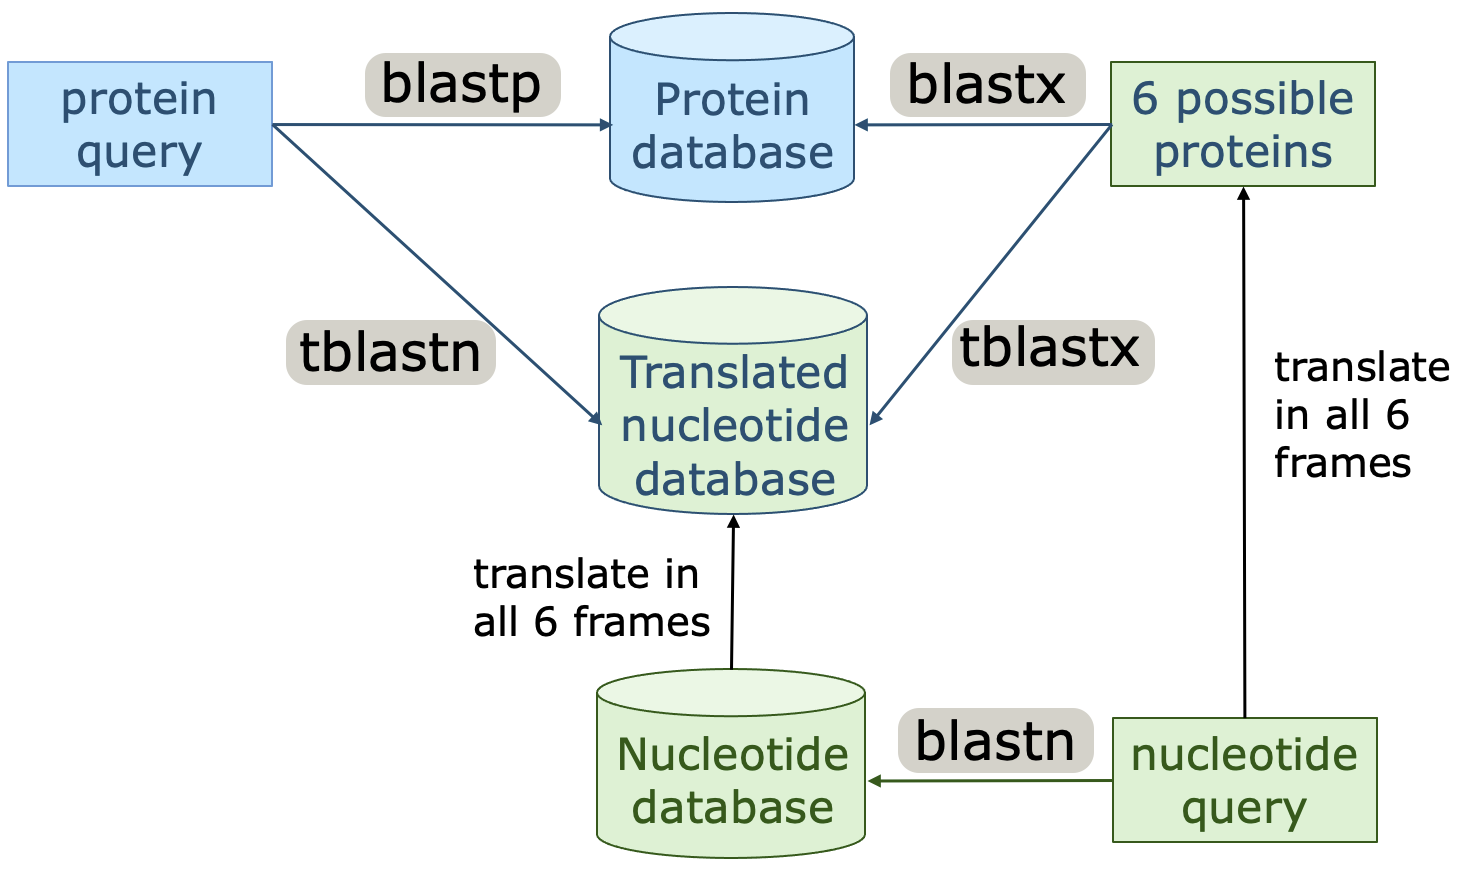
\includegraphics[width=1\linewidth]{files/blast_types-8aed2a3367dbf2bc5c263e0b04d8556e.png}
\caption[]{Different BLAST types to compare different data types. Credits: \href{https://creativecommons.org/licenses/by-nc/4.0/}{CC BY-NC 4.0} \cite{own_2_2024}.}
\label{blast_types}
\end{figure}

% #%[TODO chapter 1: File formats]

\subsection{Multiple sequence alignment}

One straightforward observation from a sequence search is that one query sequence often has multiple similar sequences (Figure~\ref{blast_output}). This can lead to research questions on for example evolution (where do these sequences come from?), function (why are some sequences more similar to each other than to others?), or structure (are all parts of these sequences equally similar/dissimilar?). To compare all of these sequences with each other using a pairwise alignment strategy would quickly lead to a large number of comparisons and would be difficult to interpret. Instead, in cases where we want to compare 3 or more sequences with each other, we turn to \textbf{multiple sequence alignment}.

The objective of performing multiple sequence alignment is to identify matching residues (DNA, RNA, or amino acids) across multiple sequences of potentially differing lengths. Similar to pairwise alignment, the result is called `a multiple sequence alignment'. The resulting multiple sequence alignment can be thought of as a square matrix: rows represent the sequences that we started with, columns represent homologous residues across sequences, and the entries are either residues or gaps (Figure~\ref{msa_concept}).

\begin{figure}[!htbp]
\centering
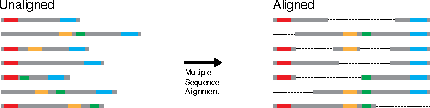
\includegraphics[width=0.8\linewidth]{files/msa-efb05f944d68f64bc1622ab87c647c51.pdf}
\caption[]{Conceptual diagram depicting multiple sequence alignment. Colored dots represent similar sequence elements, in the multiple sequence diagram on the right these elements align in vertical columns. Credits: \href{https://creativecommons.org/licenses/by-nc/4.0/}{CC BY-NC 4.0} \cite{own_2_2024}.}
\label{msa_concept}
\end{figure}

% #% INSERT: SOME SECTION ON RELEVANCE OF MSA

Various algorithms for creating multiple sequence alignments exist. Here we will go over two main concepts that are adopted by many tools: progressive alignment and iterative alignment.

\subsubsection{Progressive alignment}

To avoid having to reconcile many pairwise alignments, progressive alignment takes an iterative approach using a guide tree. The guide tree represents a crude measure of similarity between all sequences that are to be analyzed. Progressive alignment picks the two most similar sequences using the guide tree and initializes the multiple sequence alignment by aligning these two sequences with a global alignment strategy. Subsequently, the guide tree is used to determine the order in which sequences are added to the alignment. One way of thinking about this, is that progressive alignment creates increasingly large `blocks' of sequences, where a block is always treated as a unit (e.g. introducing a gap will happen for all sequences in the block). By iterating through the guide tree, this alignment strategy `progresses' to the final result, hence the name `progressive alignment'.

\begin{framed}
\textbf{Box 2.2: Constructing a guide tree}\\
The guide tree that is used by the progressive alignment strategy is typically created with a clustering algorithm that takes as input all pairwise distances between sequences. Obtaining these pairwise distances can be done through e.g. local alignment scores, but another common approach is to count the number of subsequences of length $K$ (also known as k-mers) that are present in both sequences of a sequence pair. The downside of this k-mer based strategy is that it provides a crude distance measure (and is therefore not very accurate), the benefit is that it is very fast.

In addition, once a multiple sequence alignment has been created with the progressive strategy, it is straightforward to recompute the guide tree based on this first multiple sequence alignment and calculate a second multiple sequence alignment based on this updated guide tree. This recomputing of the guide tree could in theory be repeated infinitely many times, in practice it seems sufficient to only recompute once. The often used multiple sequence alignment program \texttt{mafft} implements recomputing the guide tree in the \texttt{FFT-NS-2} algorithm.
\end{framed}

\subsubsection{Iterative refinement}

One potential downside of the progressive alignment strategy is that some of the intermediate blocks represent sub-optimal alignments. For example, when a gap is introduced during an early stage of the progressive approach, it is never removed from the alignment. Identifying and potentially improving such cases is often referred to as `iterative refinement' and typically happens on a multiple sequence alignment that was created with a progressive strategy.

Iterative refinement takes as input a multiple sequence alignment, a scoring function for the multiple sequence alignment, and a function to rearrange the multiple sequence alignment. It produces a `refined' multiple sequence alignment by rearranging the multiple sequence alignment and only keeps the new multiple sequence alignment if the score has increased. This process is typically repeated untill the score no longer increases (or for a fixed number of iterations).

Since iterative refinement methods typically start with a progressive alignment and improve its score, programs that implement an iterative refinement strategy (e.g., the FFT-NS-i method in \texttt{mafft}) typically perform better, but also need more time, than programs that are based on progressive alignment (e.g., the FFT-NS-2 method in \texttt{mafft} and the Clustal program) \cite{katoh_mafft_2014}.

\begin{framed}
\textbf{Box 2.3: Scoring and rearranging multiple sequence alignments}\\
For iterative refinement, various scoring and rearranging strategies exist. Here we outline a common approach for both: the weighted sum-of-pairs scoring function and the partitioning rearrangement strategy.

\textbf{Weighted sum-of-pairs scoring}: A generalization of the sum-of-pairs method, where the sum-of-pairs method simply calculates and sums all possible pairwise alignment scores. The generalization consists of adding specific weighing factors to each pair, where the weights are determined by the phylogenetic relationship between the sequences.

\textbf{Partitioning rearrangement}: Following a guide tree, the multiple sequence alignment is partitioned into two sub-alignments (or blocks) along each branch of the tree. Each pair of blocks is then realigned, but the resulting alignment is only kept if the score of the realigned blocks has increased.
\end{framed}

\subsection{Motifs}

Having established how to obtain a multiple sequence alignment, we now focus on several interpretations. One thing that all of these interpretations have in common, is that they enable the identification of (and search for) commonly occurring sequence patterns. A frequently used term for a commonly occurring sequence pattern is \textbf{motif}, which we will use from now on. All interpretations of motifs are based on summarizing the \textit{columns} of the multiple sequence alignment, in an attempt to describe commonly occurring residues across all sequences.

\begin{framed}
\textbf{Note 2.5: MSAs VS motifs}\\
Since all motifs are based on multiple sequence alignments, it may seem tempting to use the terms interchangeably. A key distinction is that a motif always represent a commonly occurring pattern, whereas a multiple sequence alignment can also contain regions of low conservation/similarity. In addition, one multiple sequence alignment can contain multiple motifs.
\end{framed}

Arguably the simplest representation of a motif is the \textbf{consensus sequence} (Figure~\ref{motif_concept}B), where every column of the multiple sequence alignment is represented by the most frequently occurring residue (i.e. the majority consensus). The downside of a consensus sequence is that it does not represent any of the variation present in the motif.

An extension of the consensus sequence that can represent some variation in a motif is the \textbf{pattern string} (Figure~\ref{motif_concept}C).
In pattern strings, unambigous positions are represented by single letters and there is a special syntax for representing variation:
Positions in the MSA with more than one character are represented by multiple characters in between square brackets.
A pattern string containing, for example, the pattern \texttt{[AG]} indicates that one position in the motif can be either \texttt{A} or \texttt{G}. As such, pattern strings take inspiration from \href{https://en.wikipedia.org/wiki/Regular\_expression}{regular expressions}. Various types of pattern strings exist, for example \texttt{PROSITE} \textbf{REF} strings used in the Prosite~database contain syntax for representing positions in a motif where the residue is irrelevant (marked by an \texttt{*}). Pattern strings are capable of representing some variation in the motif, but they cannot express how likely the occurence of specific variants is (in the example \texttt{[AG]}, both \texttt{A} and \texttt{G} are equally likely to occur).

To express the likelihood of a specific residue occurring at a specific position, a \textbf{Position Specific Scoring Matrix (\gls{term-pssm})} can be used (Figure~\ref{motif_concept}D).
Every row represents one of the possible characters in the MSA and every column represents a column in the MSA, where numbers indicate the probability of observing a specific character at a specific position.
Hence, every column sums to one.
For example: a DNA PSSM would have four rows, representing the nucleotides \texttt{A}, \texttt{C}, \texttt{G}, or \texttt{T}. The entries represent probabilities of observing a specific residue at a specific position. As a consequence, all columns in a PSSM must sum to one. Since a PSSM contains probabilities, it is relatively straightforward to calculate how well an unknown sequence matches an existing PSSM: assuming independence between positions, one simply multiplies the observation probabilities of the characters in the novel sequence.

Finally, sequence logos are a graphical representation of an alignment (Figure~\ref{motif_concept}E). Every position in the sequence logo represents a position in the MSA, characters are scaled proportional to their probability of being observed at their respective positions (e.g. an unambiguous position has one large character, a position with several options has multiple small characters).

\begin{figure}[!htbp]
\centering
\includegraphics[width=0.6\linewidth]{files/msa-pattern-pssm-log-5b80b466575997384e0c8bd00280fcc2.pdf}
\caption[]{Conceptual diagram depicting various representations of a conserved motif. \textbf{A:} Multiple sequence alignment (MSA) of 5 sequences and 7 positions. \textbf{B:} Consensus sequence. \textbf{C:} Pattern string. \textbf{D:} Position Specific Scoring Matrix (PSSM). \textbf{E:} Sequence logo.
Credits: \href{https://creativecommons.org/licenses/by-nc/4.0/}{CC BY-NC 4.0} \cite{own_2_2024}.}
\label{motif_concept}
\end{figure}

\subsection{Profile hidden Markov models (pHMMs)}

The previous sections on multiple sequence alignments and motifs explained some basics of how collections of similar sequences can be summarized and used. In this section we highlight a powerful approach for using the information in MSAs to perform sequence search and comparison: \textbf{profile hidden Markov models (pHMMs)}. Some of the fundamentals of general hidden Markov models (HMM) have been covered in \href{/chapter1}{Chapter 1}, here we introduce how a few simple adaptations to the general concept of HMMs unlocks a powerful sequence search approach.

The simplest introduction of profile hidden Markov models is to think of them as an extension of a position specific scoring matrix. Like a PSSM, a pHMM contains probabilities of observing certain characters at certain positions in an MSA. However, a pHMM adds the notion that the biological phenomenon of insertion and deletion of sequence elements requires unique distributions of observation probabilities. Following the hidden Markov model formulation: the \textit{hidden states} match/insert/delete all have their own unique \textit{emission probabilities} for the possible characters. In addition, a pHMM includes \textit{transition probabilities} between the  hidden states. A graphical representation of a simple profile HMM can be seen in Figure~\ref{simple_hmm}. Just like in PSSMs, a probabilistic score can be calculated for a novel sequence matching an existing HMM.
Due to the probabilistic nature of HMMs, the length of insertions is in principle unrestricted, whereas particular ranges are defined for PSSMs.
Efficient algorithms for working with pHMMs exist and have been implemented in for example the HMMer suite. The exact details of these algorithms are outside of the scope of this book.

\begin{figure}[!htbp]
\centering
\includegraphics[width=0.6\linewidth]{files/hmm-e0733ae4fec57ce5502f9917dc126281.pdf}
\caption[]{Schematic representation of a simple DNA profile HMM containing all model probabilities. The model consists of three hidden states: match (yellow square), deletion (red circle), and insertion (blue diamond). Emission probabilities are indicated inside the hidden states, transition probabilities between hidden states are indicated next to arrows.
Credits: \href{https://creativecommons.org/licenses/by-nc/4.0/}{CC BY-NC 4.0} \cite{own_2_2024}.}
\label{simple_hmm}
\end{figure}

\begin{framed}
\textbf{Box 2.4: Calculating the probability of a sequence}\\
In principle the information in Figure~\ref{simple_hmm} is enough to calculate the probability of a sequence belonging to this pHMM. For example, the sequence \texttt{GAT} would get a probability of $(0.8 * 0.6) * (0.4 * 0.7) * (0.3 * 0.4) * 0.8 = 0.013$. We arrive at this number by multiplying all relevant transition and emission probabilities. Note that determining the relevant probabilities can be more involved than in this simple example. Efficient algorithms for determining the optimal path through the HMM graph exist, but are outside of the scope of this book. In addition, we do not expect that you can perform these calculation by hand.
\end{framed}

\begin{framed}
\textbf{Sequence search with MSAs}\\
The ability to convert a multiple sequence alignment into a collection of probabilities (e.g. PSSMs or HMMs) makes it possible to calculate the probability of a novel sequence `belonging' to the multiple sequence alignment. This technique generally allows for a more sensitive approach than searching based on pairwise alignments. In practice this often means that matching sequences can be identified over larger evolutionary distances. Tools that implement some version of this approach are \texttt{psiBLAST} (which uses PSSMs) and various \texttt{HMMer} tools (all using pHMMs).
\end{framed}

\begin{framed}
\textbf{Box 2.5: pHMMs in databases}\\
The ability to group biological sequences based on conserved/co-occurring regions and subsequently using this for sequence search is exploited in a wide range of biological sequence databases. Some of these databases have been introduced in \href{/chapter1}{chapter 1}, here we briefly outline a few more details on how HMMs are incorporated into many of these resources by using Pfam as an example. All entries in the PFAM database are represented by profile HMMs. The entries are subdivided into one of six categories: family, domain, repeat, conserved site, coiled coil, or disordered. The main distinction between these six categories is the length of the matching sequences: a `family' PFAM HMM is expected to match across the entire length of a protein sequence, a `conserved site' is typically only a small region in a protein. As such, multiple PFAM HMMs can match a given protein sequence. The combination of matching PFAM HMMs on a given sequence can be used to give a fine-grained description of known elements in a sequence.
\end{framed}

\subsection{PCR primer design}

Many laborary techniques in biomedical applications rely on the polymerase chain reaction (PCR, see box 2.6) for amplifying specific fragments of DNA. Examples include pathogen detection, analyzing genetic variation, targeted mutagenesis, de novo protein synthesis, and studying gene expression patterns. Which DNA fragments are amplified is determined largely by which PCR \textit{primers} are used. To design primers that succesfully amplify the DNA of interest, several computational steps are combined. This section highlight some of these bioinformatic considerations.

\begin{framed}
\textbf{Box 2.6: The polymerase chain reaction (PCR)}\\
Invented in 1983 by Kary B. Mullis, the polymerase chain reaction was first published in 1985 in a study on sickle cell anemia \cite{saiki1985enzymatic}. Ten years after its discovery, PCR's many biomedical applications gained its inventor the 1993 Nobel prize (shared with Michael Smith for his work on site-directed mutagenesis).

As a method for amplifying DNA, PCR relies on the naturally occurring process of DNA replication by the polymerase enzyme to duplicate DNA (See Chapter~1). The reaction uses so-called primers to select which regions of DNA to amplify, and a temperature-cycling scheme to double the number of reaction products in each cycle (Figure~\ref{PCR}). PCR primers are relatively short fragments of single stranded DNA that `prime' the polymerase: they determine where DNA replication should start. Primers always come in pairs: by using a forward and reverse primer at opposing ends and strands of the desired DNA region, it is ensured that two copies of DNA can be made from one original DNA region.

During the reaction, typically three different temperature phases are alternated: (1.) the denaturation phase ({\textasciitilde}95°C) breaks up the double stranded DNA into single stranded DNA, (2.) the annealing phase ({\textasciitilde}55°C) allows the primers to bind to their complementary DNA, forming a small section of double stranded DNA, and (3.) the extension phase ({\textasciitilde}72°C) allows the polymerase enzyme to extend the double stranded section, creating two full double stranded copies of the original material. Repeating this process keeps on doubling the number of copies, which is why it is referred to as a chain reaction.
A crucial discovery in the invention of the PCR reaction for biomedical applications is the use of a polymerase enzyme that can withstand the high temperatures of the denaturation phase. The first thermostable polymerase was extracted from a species of bacteria living in hot springs: \textit{Thermus aquaticus} (hence the name \textit{Taq} polymerase).

\begin{figure}[!htbp]
\centering
\includegraphics[width=1\linewidth]{files/PCR-2730412a7c2a4e280ab9bfd52d21dbf7.jpg}
\caption[]{The polymerase chain reaction uses primers to select a desired region of DNA, and doubles it's reaction products every cycle.
Credits: \cite{PCR_NHGR}.}
\label{PCR}
\end{figure}
\end{framed}

PCR primers typically have to meet several requirements to result in a successful PCR product: they have to be biochemically feasible (i.e. denature, anneal, and extend at the right temperature), they have to be specific (only amplify the region of interest), they should produce a product of a reasonable size ({\textasciitilde}500-1000 nucleotides, depending on the application), and they should be stable as single stranded DNA. The combination of these requirements typically allows primers of {\textasciitilde}18-30 nucleotides long. To aid in the quick design of potentially successful primers, tools such as Primer-BLAST or Primer3+ automatically check most of the mentioned requirements. For example, Primer-BLAST lets a user upload a sequence of DNA that should be amplified, and can be configured to find primer products of a specific size. In addition, putative off-target amplification (i.e. specificity) is checked using BLAST on a database of choice, and several desired temperatures can be configured.

\begin{framed}
\textbf{Approximating PCR denaturation temperature $T_m$}\\
The temperature at which approximately half of the DNA strands in a solution are in a denatured stated is referred to as the \textit{melting temperature} $T_m$, and is an important parameter in primer design. The exact melting temperature depends on the exact length and nucleotide composition of the DNA fragment, but for short sequences a useful approximation exists. This approximation can come in handy for quick checks and predictions.

For primers shorter than 14 nucleotides, the melting temperature can be approximated with the following formula:

$T_m = 2 * (A + T) + 4 * (G + C)$

Where A, C, G, and T are the number of respective nucleotides in the primer.
\end{framed}


\bigskip
\centerline{\rule{13cm}{0.4pt}}
\bigskip

\subsection{Practical assignments}

This practical contains questions and exercises to help you process the study materials of chapter 2.
There are two supervised practical sessions, one on Wednesday and one on Thursday.
On the first practical day you should aim to get about halfway through this guide.
Thus, you should aim to be finished with Assignment III.
Use the time indication to make sure that you do not get stuck in one assignment.
These practical exercises offer you the best preparation for the project.
Make sure that you develop your practical skills now, in order to apply them during the project.

\textbf{Note, the answers will be published after the practical!}

\begin{framed}
\textbf{\textbf{Project Preparation Exercise}}\\
We continue the project exercise from chapter 1.
Both ARF5 and IAA5 belong to large gene families in \textit{A. thaliana}.
Now, focus on the ARF5 family and explore it by identifying homologs and looking for conserved parts among the family members.
Perform this analysis both within \textit{Arabidopsis thaliana} and outside of this species.
Assess in which plant families members are detected.

Describe the following items in a few bullet points each.
You may include up to two figures or tables.

\begin{enumerate}
\item \textbf{Materials \& Methods} What did you do? Which data, databases and tools did you use, and why did you choose them? What important settings did you select?
\item \textbf{Results} What did you find, what are the main results? Report the relevant data, numbers, tables/figures, and clearly describe your observations.
\item \textbf{Discussion \& Conclusion} Do the results make sense? Are they according to your expectation or do you see something surprising? What do the results mean, how can you interpret them? Do different tools agree or not? What can you conclude? Make sure to describe the expectations and assumptions underlying your interpretation.
\end{enumerate}
\end{framed}

\subsection{Glossary}

\subsection{References}

\section{3. Phylogenetics and tree reconstruction}

\begin{framed}
\textbf{Learning outcomes}\\
\begin{itemize}
\item 1
\item 2
\item 3
\end{itemize}
\end{framed}

In this chapter you will learn to use a \textit{Multiple Sequence Alignment} (MSA), like the ones you compiled in \href{/chapter2}{chapter 2}, and visualize the variation it contains as a phylogenetic tree.
A phylogenetic tree is considered a highly efficient \textit{data structure} summarizing the data and its variation contained in your MSA.
A tree is built from \textit{characters} which are the individual columns or positions in your MSA.
Characters have states, which are in this case the individual nucleotide or amino acid \textit{substitutions} occurring in that position (see Characters~&~trees below).
Invariable characters are columns or positions `occupied' by just one type of nucleotide or amino acid, whereas variable characters may have up to 4 different nucleotides or up to 20 amino acids per position.

% #%Create cross-link to MSA in chapter 2 when written

DNA and amino acid (AA) sequences contain the information necessary for building protein structure, comparing them in an MSA will enable insight how these structures, and their associated functions, may have changed over evolutionary times since they descended from an ancestral sequence.
The more character state changes (i.e., substitutions) occur between sequences, the more \textit{diverged} they are and probably also less related (see Related,~diverged below), and hence the further apart they will occur on your phylogenetic tree.
The information contained in your tree is hierarchical in nature, meaning that it is built-up as nested sets of subtrees that are also known as \textit{clades}.
A \textit{clade} is a group containing an ancestor together with all its descendants and is also referred to as a \textit{monophyletic} group.


\bigskip
\centerline{\rule{13cm}{0.4pt}}
\bigskip

\subsubsection{Rationale}

% :::{figure} images/chapter3/tree-of-life.png
% :alt: The Tree of Life
% :width: 40%
% :name: tree_of_life
% align: center
% The Tree of Life. Dated in millions of years; \
% rooted with Eubacteria. Credits: {cite}`tree_of_life_2022`.
% :::
% #% Unable to use figure tree_of_life due to copyright.

\begin{figure}[!htbp]
\centering
\includegraphics[width=0.5\linewidth]{files/tree-of-life_alt-af7529eddf9e121b8f98d25d1b99b119.png}
\caption[]{Simplified Tree of Life. Credits: \newline
\href{https://creativecommons.org/licenses/by/4.0/}{CC BY 4.0} \cite{tree_of_life_alt_2014}.}
\label{tree_of_life_alt}
\end{figure}

Why should we study phylogenetics and what is it about?
Ever since Darwin we know that all living things are connected in a tapestry of life, forming a phylogenetic tree of everything (Figure~\ref{tree_of_life_alt}).
Phylogenetics aims at understanding evolutionary relationships among genes, species, and higher taxa and as such it is relevant to almost all biological questions.
Why? Because an evolutionary context (rather than a `snapshot' perspective) allows identifying evolutionary lineages and their origins, and can provide information on how lifeforms and sequences change and adapt across millions of years.
Examples are studying the evolution of gene families within genomes, or the build-up of species relationships in a lineage.

\begin{figure}[!htbp]
\centering
\includegraphics[width=1\linewidth]{files/sars-cov-2-c625ea5bfa5a5808c0ab8b5230606e98.svg}
\caption[]{The SARS-CoV-2 phylogenetic tree, March 2024.
Credits: \href{https://creativecommons.org/licenses/by/4.0/}{CC BY 4.0} \cite{sars-cov-2_2018}.}
\label{sars-cov-2}
\end{figure}

Other examples are studying Covid-19 and other pathogen outbreaks (Figure~\ref{sars-cov-2}), studying molecular evolution and the accumulation of substitutions in a multiple sequence alignment (MSA).
Or, studying population history within a species, reconstructing historical biogeography: In all these cases having an \textit{accurate phylogenetic tree} is crucial, because we want to be able to reconstruct evolutionary lineages (the branches in phylogenetic trees) and how they evolved, changed, duplicated, or went extinct.
By \textit{accurate} we mean estimating relationships that are as close as possible to the actual (historic) relationships, which we cannot know for sure.
As they happened in the past we cannot \textit{prove} them, but they are hypotheses (of relationships) that we can only \textit{corroborate} (confirm, seek support for).

% :::{figure} images/chapter3/ancestral-states.png
% :alt: A phylogenetic tree with ancestral states
% :width: 100%
% :name: ancestral_states
% 
% Comparing species (or genes) in a phylogenetic tree allows inference of ancestral states and evolutionary trends.
% :::
% #% Unable to use figure ancestral_states because of poor quality

\begin{figure}[!htbp]
\centering
\includegraphics[width=1\linewidth]{files/ancestral-states_alt-7d2c296e2211f343a7dbc95928147ca9.pdf}
\caption[]{Comparing species (or genes) in a phylogenetic tree allows inference of ancestral states and evolutionary trends.
Credits: \href{https://creativecommons.org/licenses/by-nc/4.0/}{CC BY-NC 4.0} \cite{own_3_2024}.}
\label{ancestral_states_alt}
\end{figure}

When a phylogenetic tree is known for a specific group, and it is properly rooted, the \textit{ancestral states} for its characters can in principle be reconstructed (for instance the ancestral amino acid residues in a protein sequence) for each node in the tree.
With that, \textit{evolutionary trends} (towards current conditions) can be inferred, enabling the study of character evolution, i.e., how things change over time (Figure~\ref{ancestral_states_alt}).


\bigskip
\centerline{\rule{13cm}{0.4pt}}
\bigskip

\subsubsection{Phylogenetic trees: structure \& interpretation}

Like all trees, phylogenetic trees come with a stem, branches, leaves and ideally a root.
What makes phylogenetic trees special however is that they are actually hypotheses of evolutionary relationships, as outlined in the previous section.
The leaves or external nodes are then the individuals (or sequences) that are observed and compared, which are also referred to as \textit{operational taxonomic units} (OTUs) or \textit{terminals}.
The branches and nodes are the \textit{lineages} or \textit{clades} that are inferred, i.e., not observed.
A clade is an ancestral node together with all its descendants, which is also referred to as a \textit{monophyletic} group.
They are recognised by the horizontal lines connecting the OTUs and HTUs (hypothetical taxonomic units) in your phylogenetic tree, as for instance shown in Figure~\ref{tree_example}.

\begin{figure}[!htbp]
\centering
\includegraphics[width=1\linewidth]{files/tree-example-8bf61d496e001c2421255111571c4c29.png}
\caption[]{A rooted ultrametric phylogenetic tree with its main parts and characteristics indicated.
Here, the OTUs are GenBank plant chloroplast gene accessions, the names of which have been condensed.
Credits: \href{https://creativecommons.org/licenses/by-nc/4.0/}{CC BY-NC 4.0} \cite{own_3_2024}.}
\label{tree_example}
\end{figure}

Whereas the horizontal lines represent the actual branches, the vertical lines do not have a meaning and are just there to connect the branches and clades; they will get longer when more terminals are included but do not have a relation with the data (i.e., the MSA).
Branches are connected via nodes, that can be internal (HTUs) or external (OTUs).
\textit{Internal nodes} represent \textit{hypothetical ancestors} that are not observed or sequenced but inferred or reconstructed.
As outlined above, \textit{external nodes} are the actual \textit{individuals} observed; they are never connected directly to each other, only through internal nodes.
These individuals can represent genes, species or higher taxa, but they are never categories (or averages), as characters and states are indivisible observations scored on individuals.
Branches and nodes collectively build the \textit{tree topology}, i.e., the structure of the tree.

One of the most important aspects of a phylogenetic tree is whether it is rooted, meaning whether we can distinguish which nodes are old and which are more recent, and also what \textit{clades} are present.
Rooting is done by selecting an \textit{outgroup}, which is a reference taxon outside the group of interest (this is described in more detail in section Rooting~&~clades).
It is important to realise that most phylogenetic reconstruction methods actually produce unrooted trees, which can then rooted using an outgroup to visualize in what direction evolution proceeded and which clades can be identified.


\bigskip
\centerline{\rule{13cm}{0.4pt}}
\bigskip

\paragraph{Related, diverged}\label{chapter3_related_diverged}

% :::{figure} images/chapter3/MRCA-mammals.png
% :alt: An additive phylogenetic tree rooted at monkey
% :width: 100%
% :name: MRCA_mammals
% 
% Additive phylogenetic tree of mammalian species, rooted on monkey.
% The MRCA of monkey, cat and dog is indicated.
% Tree topology informs relatedness, branch lengths correspond to divergence. Credits: modified from {cite}`bioinformatics_2007`.
% :::
% #%Imagery from this source (Zvelebil and Baum, 2007) is under copyright, unable to be used.

\begin{figure}[!htbp]
\centering
\includegraphics[width=1\linewidth]{files/MRCA-mammals_alt-0cb54f582d195996e5a3b6cd93ee9a57.pdf}
\caption[]{Additive phylogenetic tree of mammalian species, rooted on monkey.
The MRCA of monkey, bear, seal and dog is indicated.
Tree topology informs relatedness, branch lengths correspond to divergence.
Credits: \href{https://creativecommons.org/licenses/by-nc/4.0/}{CC BY-NC 4.0} \cite{own_3_2024}.
Made using imagery from: \href{https://creativecommons.org/licenses/by/4.0/}{CC BY 4.0} \cite{DBCLS_2023}}
\label{MRCA_mammals_alt}
\end{figure}

In a rooted phylogenetic tree, terminals sharing a more recent common ancestor are more closely related than terminals sharing a less recent common ancestor.
Thus, in Figure~\ref{MRCA_mammals_alt}, dog and bear are more related than dog and seal, because dog and bear share a more recent common ancestor.
On the other hand, monkey and dog are as related as monkey and cat, because they all share the same \textit{most recent common ancestor} (MRCA).
Being \textit{related} is not the same as being \textit{diverged}, as divergence means the amount of change accumulated since the split of two lineages, which is reflected in the branch lengths (or in distances).
In our example, raccoon and dog would be more diverged than raccoon and bear, but not more closely related.


\bigskip
\centerline{\rule{13cm}{0.4pt}}
\bigskip

\paragraph{Cladogram, additive and ultrametric}\label{chapter3_cladogram_additive_ultrametric}

Phylogenetic trees come in three flavors: \textit{ultrametric}, \textit{additive}, and \textit{cladogram}.
When all paths starting from the root to each external node are of equal length, you could interpret the length of a path through the tree as proportional to time and thus equally old as other paths; the ages of nodes can then in principle be inferred.
Such a tree is known as an \textit{ultrametric} tree, which can be easily recognised by its topology in which all terminal branches line up, usually to the right.
Another, more common type of phylogenetic tree is the \textit{additive} tree, in which branch lengths are proportional not to time but to the amount of change occurring in your data set (the MSA).
Therefore, the more changes (i.e., substitutions, insertions, deletions) occur for an individual, the longer the branch to its MRCA will be in the additive tree.
Most phylogenetic and tree building platforms or software packages produce additive trees.
Producing ultrametric trees usually requires taking extra steps, with each step introducing uncertainty.
You could argue that ultrametric trees are \textit{one extra step away from the data} compared to additive trees.
Only when the data accumulates substitutions in a strictly clock-like manner (i.e., like radio-active decay) would the ultrametric and additive tree version be the same.
However, such strict molecular clocks are never encountered in real data.
Finally, a \textit{cladogram}-style tree is a `schematic tree' meant to only show the topology of your tree.
It therefore has artificial (equal) branch lengths, including for terminal branches.

\begin{figure}[!htbp]
\centering
\includegraphics[width=1\linewidth]{files/tree-types-6565f30c28375a5d8adf5ad524b5b3db.png}
\caption[]{A rooted phylogenetic tree with its main parts and characteristics indicated.
Here, the OTUs are GenBank plant chloroplast gene accessions, the names of which have been condensed.
For the same data, the tree is given as \textit{additive} tree (top) and as an \textit{ultrametric} tree (bottom left) with branch lengths corresponding to time.
On the right, flipped, the same tree as \textit{cladogram}, with branch lengths only indicating the structure of the trees.}
\label{tree_types}
\end{figure}

% #% This figure could be much clearer in depicting additive trees and cladograms.


\bigskip
\centerline{\rule{13cm}{0.4pt}}
\bigskip

\paragraph{Tree resolution}

The resolution of a phylogenetic tree is the extent to which nodes and branches (clades) can be inferred/observed from the tree.
Trees can be \textbf{fully} resolved, in which case each internal node is connected to three branches: the ancestral branch and two subtending branches.
Such trees are called \textit{bi-furcating} or \textit{dichotomous}, meaning that each branch splits into two and there are no uncertainties on branching order or resolution of nodes.
Frequently however, phylogenetic trees will be \textit{partly resolved} and contain \textit{polytomies}, which are nodes connected to (many) more than three branches.
Polytomies represent parts of the phylogenetic tree that are uncertain in terms of branching order of the lineages involved.
This can be due to there being insufficient information in the MSA for resolving the lineages, or ample but conflicting signal.
Polytomies are usually interpreted as \textit{soft}, meaning that the data used does not allow to resolve the lineages inferred (Figure~\ref{polytomies_alt}).

% :::{figure} images/chapter3/polytomies.png
% :alt: Hard and soft polytomies
% :width: 60%
% :name: polytomies
% 
% Hard and soft polytomies in a phylogenetic tree.
% The soft polytomy can imply different tree resolutions. Credits: {cite}`phylogenetic_approach_1998`.
% :::
% #% Unable to use figure polytomies due to copyright.

\begin{figure}[!htbp]
\centering
\includegraphics[width=0.6\linewidth]{files/polytomies_alt-05648f03f11a7f84726ae227c73aa2f6.pdf}
\caption[]{Hard and soft polytomies in a phylogenetic tree.
The soft polytomy can imply different tree resolutions.
Credits: \href{https://creativecommons.org/licenses/by-nc/4.0/}{CC BY-NC 4.0} \cite{own_3_2024}.}
\label{polytomies_alt}
\end{figure}

In contrast, the \textit{hard} interpretation would be: instantaneous speciation, i.e., an ancestral species lineage split up so fast that the new lineages do not have sufficient unique substitutions to `mark' them and to assign them an internal node in the tree.
An example is the late-Tertiary radiation of mammalian orders, after the fairly quick establishment of cold water around the Earth's poles, combined with that of the hot tropics.
Several published mammalian phylogenetic trees contain unresolved spines or backbones.

On the other hand, gene~trees (used for studying gene families) may also contain polytomies and they are usually considered as soft (the data is not decisive enough to infer a branching order).
\textit{Whole genome duplications} (auto-polyploidisations) are fairly well known, especially in the evolution of flowering plants. Following such an event, pairs of genes can be expected to form instantaneously, i.e., without accumulating unique substitutions, and may result in hard polytomies in gene trees.


\bigskip
\centerline{\rule{13cm}{0.4pt}}
\bigskip

\paragraph{Orthologs \& paralogs}\label{chapter3_orthologs_paralogs}

When the terminals included are actually \textit{gene} or \textit{protein sequences}, the tree will be a \textit{gene tree}, likely containing \textit{homologs} (derived from a common ancestor gene), possibly also \textit{orthologs} and \textit{paralogs}.
\textit{Orthology} is the occurrence of corresponding, homologous (and mostly similar), genes in lineages resulting from speciation.
For instance, human beta globin and chimp beta globin are orthologs.
Usually, these genes will have the same function in different species, but this doesn't necessarily have to be the case.
In contrast, \textit{paralogy} is the occurrence of similar genes resulting not from speciation but from gene duplication.
For example, proteins from a gene family with different functions in the same species. Such similar genes are referred to as \textit{paralogs}, which are visualized as multiple occurences of particular terminals on the tree.
Figure~\ref{ortho_para}A and B illustrates the process of gene duplication followed by speciation, resulting in two parallel subtress (the grey X tree and the green X' tree). Figure~\ref{ortho_para}C shows the challenge with using both orthologs and paralogs in phylogenetic analysis when not all members of a gene family have been sampled.

\begin{figure}[!htbp]
\centering
\includegraphics[width=1\linewidth]{files/ortho-para-df6a4f2e797aa9f7fb70f004212067f5.pdf}
\caption[]{The challenge of paralogs: (A) Paralogous genes are created by gene duplication events.
Gene X is duplicated in a (recent) common ancestor (RCA) of species A and B resulting in paralogous genes X and X'.
Species A and B inherit both copies of the gene (unless one or the other is lost somewhere along the way).
(B) Phylogenetic analysis of the X/X' gene family gives two parallel phylogenies.
All sequences of gene X are orthologues of each other, as are all sequences of gene X'.
However, X and X' are paralogues.
Both the X and X' subtrees show the true relationships among the three species.
The subtrees are also each other's natural outgroup, and as a result each subtree is rooted with the other (reciprocally rooting).
(C ) A tree of the X/X' gene family can be misleading if not all the sequences are included (because of incomplete sampling or gene loss).
If the broken branches are missing, then the true species relationships are misrepresented.
Credits: \href{https://creativecommons.org/licenses/by-nc/4.0/}{CC BY-NC 4.0} \cite{own_3_2024}.}
\label{ortho_para}
\end{figure}

In Figure~\ref{gene_duplication_speciation_alt}, a sequence of events is given involving \textit{two duplications and one speciation event} that can lead to a set of homologous genes in two species.
Some of these are \textit{orthologs} and some are \textit{paralogs} that have acquired new functions.
A species tree is depicted by the pale blue cylinders, with the branch points (nodes) in the cylinders representing speciation events.
In the ancestral species (on top) a gene is present as a single copy and has function $\alpha$ (blue).
After some time, a gene duplication event occurs within the genome, producing two identical gene copies, one of which subsequently evolves a different function, identified as $\beta$ (red).
As a result, $\alpha$ and $\beta$ are now paralogous genes.
Later on, a speciation event occurs resulting in two species (A and B), both containing genes $\alpha$ and $\beta$.
Gene B$\alpha$ (in species B) subsequently undergoes another duplication event, resulting in the paralogous genes B$\alpha$ and B$\gamma$.
After further divergent evolution, B$\gamma$, aquires a new function $\gamma$ (green).
The B$\alpha$ gene is still functionally very similar to the original gene $\alpha$.
At the end of this period of evolution, all five genes in the two species are homologous, with three orthologous pairs: A$\beta$/B$\beta$, A$\alpha$/B$\alpha$, and A$\alpha$/B$\gamma$.
The B$\alpha$ and B$\gamma$ genes are paralogous, as are any other combinations except the orthologous pairs.
Note that A$\alpha$ and B$\gamma$ are orthologs despite their different functions.
The gene tree inferred from these five genes has multiple occurrences of both species A and B (Figure~\ref{gene_duplication_speciation_alt}B).

% :::{figure} images/chapter3/gene-duplication-speciation.png
% :alt: Evolutionary history of a gene after duplication and speciation events.
% :width: 100%
% :name: gene_duplication_speciation
% 
% The evolutionary history of a gene that has undergone two separate duplication events.
% (A) The species tree (large blue cylinders) comprising species A and B and with indicated gene duplication and neo-functionalisation events leading to β and γ functions.
% (B) The phylogenetic tree that would be drawn for the resulting 5 genes in (A), here drawn as a cladogram. Credits: {cite}`bioinformatics_2007`.
% :::
% #% Unable to use figure gene_duplication_speciation due to copyright

\begin{figure}[!htbp]
\centering
\includegraphics[width=1\linewidth]{files/gene-duplication-spe-54222efe84d06eec938ca9305ffe33d6.pdf}
\caption[]{The evolutionary history of a gene that has undergone two separate duplication events.
(A) The species tree (large blue cylinders) comprising species A and B and with indicated gene duplication and neo-functionalisation events leading to $\beta$ and $\gamma$ functions.
(B) The phylogenetic tree that would be drawn for the resulting 5 genes in (A), here drawn as a cladogram.
Credits: \href{https://creativecommons.org/licenses/by-nc/4.0/}{CC BY-NC 4.0} \cite{own_3_2024}.}
\label{gene_duplication_speciation_alt}
\end{figure}

For another example of a gene versus species tree consider the trees in Figure~\ref{IL_tree_alt}, which are based on the comparison of Interleukin gene sequences.
There are multiple occurrences of the terminals from the species tree (bovine, sheep, pig etc.) in the gene tree, each grouped with a different Interleukin sequence type.
These are the paralogs, that probably resulted from gene duplication events during the proliferation of the IL clade.

Given that there are four copies of IL1 in humans (indicated with green boxes in the gene tree in Figure~\ref{IL_tree_alt}), there must have been at least three gene duplications in the history of the interleukins.
Three of them are inferred from the presence of multiple copies of IL in the same mammalian species, i.e. i) in the ancestor of the IL-1$\alpha$ + $\beta$ clade, ii) in the ancestor of the IL-1r$\alpha$ + $\beta$ clade, and iii) as a sister pair in the IL-1$\beta$ clade.
Duplication $\delta$3 is required to explain the incongruence between the mammalian species tree and the IL-1$\beta$ phylogeny.
The incongruence is that in the gene tree human and mouse are more closely related than either is to bovine/sheep.
The species tree however indicates human to be more closely related to bovine/sheep than to mouse.
In order to resolve (reconcile) this, $\delta$3 is suggested as indicated in Figure~\ref{IL_reconciled_alt}.

% In fact, we can deduce that four gene duplication events must have happened, to explain the occurrence of for instance 'human' at three positions in the gene tree (indicated with green boxes in {numref}`IL_tree_alt`), namely I) in the IL-1α clade, II) in the IL-1rα clade, and III) as a sister pair in the IL-1β clade.
% The fourth duplication event would be necessary to assume to explain the IL-1β versus IL-1βm copies.
% All gene copies in this tree are homologs, some are orthologs (e.g., Human IL-1β and Mouse IL-1β), and some are paralogs (e.g., Human IL-1β and Human IL-1βm).

% :::{figure} images/chapter3/IL-tree.png
% :alt: Species tree and a gene tree of mammalian Interleukin-1 genes.
% :width: 100%
% :name: IL_tree
% 
% A species tree based on external evidence (left) and a gene tree based on a comparison of mammalian Interleukin-1 genes (right).
% In the gene tree, both alpha and beta copies can be seen, which are probably the result of gene duplications (see {numref}`gene_duplication_speciation_alt`). Credits: {cite}`phylogenetic_approach_1998`.
% :::
% #% Unable to use figure IL_tree due to copyright.

\begin{figure}[!htbp]
\centering
\includegraphics[width=1\linewidth]{files/IL-tree_alt-d1fbb3f9a9055084ebcab692bcba592f.pdf}
\caption[]{A species tree based on external evidence (left) and a gene tree based on a comparison of mammalian Interleukin-1 genes (right).
In the gene tree, both alpha and beta copies can be seen, which are probably the result of gene duplications (see Figure~\ref{gene_duplication_speciation_alt}).
Occurrences of `Human' in the gene tree are indicated with green boxes.
Credits: \href{https://creativecommons.org/licenses/by-nc/4.0/}{CC BY-NC 4.0} \cite{own_3_2024}.
Made using imagery from: \href{https://creativecommons.org/licenses/by/4.0/}{CC BY 4.0} \cite{DBCLS_2021}.}
\label{IL_tree_alt}
\end{figure}

The tree in Figure~\ref{IL_reconciled_alt} is a so-called \textit{reconciled tree}, which has been inferred as an \textit{extended tree} that would be necessary to assume in order to explain the position and distribution of all IL sequence types in the gene tree.
Apart from four gene duplications (marked $\delta$\textsubscript{1}, $\delta$\textsubscript{2}, $\delta$\textsubscript{3} and $\delta$\textsubscript{4}), several \textit{gene losses} (indicated with light grey branches) too would need to be assumed to explain the pattern in the gene tree in Figure~\ref{IL_tree_alt}.

% :::{figure} images/chapter3/IL-reconciled.png
% :alt: A reconciled tree of the species tree and gene tree of mammalian Interleukin-1 genes.
% :width: 100%
% :name: IL_reconciled
% 
% Reconciled tree for the mammalian interleukin-1 gene tree shown in {numref}`IL_tree_alt`.
% Gene losses are indicated in light grey. Of the four duplications required, three are supported by the presence of multiple copies of IL in the same mammal species, and one (δ{sub}`3`) is required to explain the incongruence between IL-1 and mammalian phylogeny. Credits: {cite}`phylogenetic_approach_1998`.
% :::
% #% Unable to use figure IL_reconciled due to copyright.

\begin{figure}[!htbp]
\centering
\includegraphics[width=0.6\linewidth]{files/IL-reconciled_alt-f4622dda751c1e5d8897ab8ec85ab066.pdf}
\caption[]{Reconciled tree for the mammalian interleukin-1 gene tree shown in Figure~\ref{IL_tree_alt}.
Gene losses are indicated in light grey.
Of the four duplications required, three are supported by the presence of multiple copies of IL in the same mammal species, and one ($\delta$\textsubscript{3}) is required to explain the incongruence between IL-1 and mammalian phylogeny.
Credits: \href{https://creativecommons.org/licenses/by-nc/4.0/}{CC BY-NC 4.0} \cite{own_3_2024}.}
\label{IL_reconciled_alt}
\end{figure}

\begin{framed}
\textbf{Box 3.1: Species tree estimation analysis.}\\
\begin{figure}[!htbp]
\centering
\includegraphics[width=0.4375\linewidth]{files/embedded-tree-64ef7ee5f957a172953a19139f9aad89.png}
\caption[]{Gene trees, in color, embedded in the \newline
species tree (black lines) of western \newline
pocket gophers (\textit{Geomyidae, Thomomys}). \newline
Credits: \href{http://creativecommons.org/licenses/by-nc/2.5}{CC BY-NC 2.5} \newline
\cite{embedded_tree_2009}.}
\label{embedded_tree}
\end{figure}

When terminals are individuals meant to represent species, we would in principle be inferring a \textit{species tree}.
Figure~\ref{embedded_tree} shows an example of multiple gene trees (in color) contributing to the species tree (indicated by black lines) as a result of \textit{species tree estimation analysis}.
The different species names, in this case \textit{Thomomys} `Western pocket gophers' (Geomyidae), are indicated along the horizontal axis and their \textit{coalescence} (gene lineages coming together, looking backwards in time) can be traced through time.
Such analysis is beyond the scope of this course, but it is of course important to always keep in mind at what level your phylogenetic reconstruction is, whether at the species, gene, or even biogeographic area level.
\end{framed}


\bigskip
\centerline{\rule{13cm}{0.4pt}}
\bigskip

\paragraph{Nodal support in phylogenetic trees: the bootstrap}\label{chapter3_bootstrap}

Not all parts of a phylogenetic tree will be equally well-supported or strong, given our character data (MSA).
There can be considerable uncertainty around the estimated nodes of our tree, affecting the confidence we have in those nodes.
In experimental science, usually some statistic measure is used to quantify uncertainty, for instance the mean and standard deviation of outcomes of repeated experiments.
Phylogenetics, however, is not experimental but rather seeks to reconstruct historic patterns that were driven/shaped by evolution.
As outlined at the beginning of this chapter, the implication is that we cannot \textit{prove} phylogenies, nor repeat them, or even know whether we reconstructed the correct one.
We `only' have our phylogenetic trees as estimates of the \textit{true phylogeny}.

In order to measure support for the nodes in our phylogenetic tree, rather than producing several replicates of our MSA (which will most likely all be identical), we can draw random samples from the MSA and use these \textit{pseudo-replicate} data sets to build trees (Figure~\ref{bootstrap_resampling_alt}).
Repeating this process many times (hundreds or thousands) and summarizing the variation among the trees thus reconstructed, provides insight in the structure of our data and how it supports the nodes in a tree.
It actually measures the sampling \textit{variance about the estimate} of the phylogeny Figure~\ref{bootstrap_resampling_alt}B.
This process is called \textit{bootstrap analysis} and will be further discussed in Maximum~likelihood~tree~building, after we have covered the \textit{characters} underlying our trees in the next section.

% :::{figure} images/chapter3/bootstrap-resampling.png
% :alt: Comparison between an unlimited and limited data bootstrap resampling analysis approach.
% :width: 100%
% :name: bootstrap_resampling
% 
% Bootstrap resampling analysis in phylogeny reconstruction.
% In case of unlimited data (A), not realistic, a summary of sample-based trees yields sampling variance about the **true phylogeny**.
% In case of limited data (B), realistic, only pseudo-samples are available, that summarise sampling variance about the **estimate of true phylogeny**.
% :::
% #% Unable to use figure bootstrap_resampling due to copyright.

\begin{figure}[!htbp]
\centering
\includegraphics[width=1\linewidth]{files/bootstrap-resampling-a3f842b3087cc8c4bf2b3a49cf266841.pdf}
\caption[]{Bootstrap resampling analysis in phylogeny reconstruction.
In case of unlimited data (A), not realistic, a summary of sample-based trees yields sampling variance about the \textit{true phylogeny}.
In case of limited data (B), realistic, only pseudo-samples are available, that summarise sampling variance about the \textit{estimate of true phylogeny}.
Credits: \href{https://creativecommons.org/licenses/by-nc/4.0/}{CC BY-NC 4.0} \cite{own_3_2024}.}
\label{bootstrap_resampling_alt}
\end{figure}


\bigskip
\centerline{\rule{13cm}{0.4pt}}
\bigskip

\subsubsection{Characters \& trees}\label{chapter3_characters_trees}

As outlined above, phylogenetic trees are not directly observed but \textit{inferred}, and represent hypotheses of evolutionary relationship, grouping individuals on the basis of shared history.
The data used for comparison are the homologous sites among a set of sequences (amino acid or nucleotide) that have been aligned in an MSA in which substitutions are made visible.
\textit{Homologous} here means that there are corresponding positions in a gene sequence that are due to common ancestry.
So, for instance, position 423 in a gene sequence from one species is homologous with position 423 in that of another species, because both species shared a recent common ancestor and we assume the genes to be orthologs.
Each such position is considered a character with states that are efficiently visualized in an MSA as \textit{substitutions} (Figure~\ref{MSA_alt}A).
All nucleotide or amino acid substitutions in the MSA, both unique ones (occurring in only a single individual or sequence) and shared ones (occurring in at least two sequences), are used to build the phylogenetic tree.
Invariant characters however, showing no substitutions, are not expected to contribute to the tree building process as they do not contain comparative signal.
Shared substitutions are informative for building the branches of your tree, as they group terminals and hence add to the length of internal branches.
Unique substitutions on the other hand only contribute to the \textit{twigs} or external branch lengths and have no grouping power.
The more shared substitutions occur for a set of sequences in your MSA, the stronger the resulting node in the phylogenetic tree will be supported.

\begin{figure}[!htbp]
\centering
\includegraphics[width=0.8\linewidth]{files/MSA_alt-889d2d785b8a5eb2edc29091c0208524.pdf}
\caption[]{Characters and trees.
\textbf{A}: Multiple sequence alignment (MSA, nucleotides) with examples of shared-derived (S), unique (U) as well as invariant (I) characters indicated; \textbf{B}: MSA containing S, U and I characters and the number of steps per character, as well as the total tree length for tree1 and tree2 indicated on the bottom lines.; \textbf{C}: two `candidate trees' as alternative hypotheses explaining the data in the MSA in (B), with character state changes for all characters are indicated on the trees and exemplar syn- and autapomorphies are indicated.
Note that character 6 is invariant and therefore does not contribute to any tree.
Tree 1 requires one step less than tree2 and is therefore the preferred tree.
Credits: (A) created using MEGA11 and modified from \cite{mega_2021} (B \& C) \href{https://creativecommons.org/licenses/by-nc/4.0/}{CC BY-NC 4.0} \cite{own_3_2024}}
\label{MSA_alt}
\end{figure}

When observing substitutions in an MSA we cannot say which ones are ancestral (occurring already in `deep' ancestors) and which ones are derived, occurring more recently.
But placed in the context of a rooted phylogenetic tree, shared substitutions can actually be shared derived substitutions, which are known as \textit{synapomorphies} (\textit{syn}=shared, \textit{apo}=derived, \textit{morphy}=character), whereas uniquely derived substitutions are called \textit{autapomorphies} (see Figure~\ref{MSA_alt}B \& C).

When designing a phylogenetic study, involving the compilation of one or more MSAs, there is usually a choice between adding more \textit{characters} (lengthening the MSA) versus adding more \textit{terminals} (adding more sequences(rows) to the MSA).
Whereas the former is tempting, it is often more useful to add terminals (taxa) as this allows extra synapomorphies to be realised.
After all, synapomorphies are relative (not absolute) entities: only in the context of other sequences can you actually `see' them.
For instance, when studying a gene family in which duplications have occurred during the evolution of its lineages, many taxa should be included in the MSA in order to capture the duplication events.
Only adding more characters may amplify errors or artefacts caused by taxic under-sampling.
This can lead to incorrectly inferred long branches with seemingly high support for their position and nodes.
This phenomenon is referred to as long-branch attraction and is discussed further in Estimating~sequence~divergence.


\bigskip
\centerline{\rule{13cm}{0.4pt}}
\bigskip

\paragraph{Rooting \& clades}\label{chapter3_rooting_clades}

A \textit{clade} is an ancestral node together with all its descendants, which is also referred to as a \textit{monophyletic group}.
We usually refer to the ancestral node of a clade as the inferred \textit{most recent common ancestor} (MRCA).
Of course, there will always be less recent (`deeper') ancestors but they will probably not be informative for recognising and inferring a clade and its relationships, as they are also the ancestor of other clades.
At deep divergences (e.g., herring \textit{versus} fruit fly), homology and resolution of the characters used may not be clear and sufficient.

Information contained in phylogenetic trees is \textit{hierarchical}, with structures being part of other, more inclusive, ones.
Clades are indeed usually nested into each other, i.e., a clade is a subset of a larger clade.
Apart from being nested, clades can also be each other's \textit{sisters}, which means they share an exclusive most recent common ancestor (MRCA) with no other clades included (Figure~\ref{nested_clades_alt}).
Such \textit{sister groups} are highly useful in, for instance, evolutionary and comparative studies, as they represent lineages of exact equal age.

% :::{figure} images/chapter3/nested-clades.png
% :alt: A depiction of a rooted nested tree and nested and sister clades with MRCA.
% :width: 100%
% :name: nested_clades
% 
% Nested clades and sister clades.
% Left, the same rooted tree as in {numref}`rooted_trees`, now with nested clades indicated by orange shapes: the small orange clade is nested in the lager orange one; it is also a sister clade of the green clade; as are the blue and large orange shapes. Credits: modified from {cite}`bioinformatics_2007`.
% Right, nested and sister clades with LCA (last common ancestor = MRCA) indicated. Credits: modified from {cite}`nested_clades_2014`.
% :::
% #% Unable to use figure nested_clades due to copyright.

\begin{figure}[!htbp]
\centering
\includegraphics[width=1\linewidth]{files/nested-clades_alt-56131360ec06dc90e0c4ed033e7b1795.pdf}
\caption[]{Nested clades and sister clades.
Top, the same rooted tree as in Figure~\ref{rooted_trees_alt}, now with nested clades indicated with orange and green shapes: the small orange clade is nested in the larger -dashed- one; it is also a sister clade of the green clade; as are the blue and larger dashed clades.
Bottom, nested and sister clades with MRCA indicated.
Credits: \href{https://creativecommons.org/licenses/by-nc/4.0/}{CC BY-NC 4.0} \cite{own_3_2024}.}
\label{nested_clades_alt}
\end{figure}

Again, an MRCA together with \textit{all} its descendants is considered to form a clade.
Such a clade can then be the basis of further analysis or classification.
It is good to realise that the clade is based on observations (synapomorphies) and therefore represents \textit{evidence}, whereas classification is in principle subjective (\textit{opinion}) and an interpretation and use of the clade.
For instance, when any descendant of a clade is left out in a classification, for example \textit{Vertebrates} being left out from the \textit{Invertebrates}, or birds left out from dinosaurs, the proposed taxon or classification is not monophyletic anymore and is considered a \textit{paraphyletic group} (i.e., an MRCA and \textit{not all} its descendants).
Paraphyletic groups (also referred to as \textit{non-natural groups}) are still in use but not considered to be a proper basis for classification.

When studying gene families and their evolution, it is useful to make comparisons among clades in the gene tree, especially among sister clades, as they are of exactly the same age.
Any differences between them, in terms of substitution rates, sequence bias in composition, or the number of lineages per clade, is then due to speciation processes, not the different age of the clades.
In order to make these comparisons it is important to compare monophyletic and not paraphyletic groups as the latter are not directly comparable or of equal age.

\textit{Rooting} a tree is polarising it, making a distinction in what are old and younger nodes.
When a tree is properly rooted, usually with an outgroup reference taxon outside the group of interest, it is therefore directed in terms of ancestry and clades can be inferred (see Figure~\ref{rooted_trees_alt}B; Note that unrooted trees, which are non-polarised, in principle do not contain clades but `clans').
In the example in Figure~\ref{rooted_trees_alt}, B, we see that the rooted version of the bird phylogenetic tree seems to contain one extra brown bird.
External evidence (which is not shown in the figure, only the vertical branch on top leading to the outgroup) was apparently convincing in placing the root between the white and brown birds.
Thus, a new, internally placed, brown bird is inferred as the MRCA, to which the outgroup branch can attach.
This however makes the brown birds paraphyletic with regards to the white birds, because not all descendants from the brown MRCA are brown, some are white.
The white birds themselves are now monophyletic.

% :::{figure} images/chapter3/rooted-trees.jpg
% :alt: Unrooted and rooted tree depictions.
% :width: 100%
% :name: rooted_trees
% 
% Rooting phylogenetic trees.
% (Left) Unrooted tree depicting phylogenetic relationships among a set of yellow and brown bird species; external nodes represent the extant (living, observed) species, each with their morphological synapo- or autapomorphies, the internal nodes represent inferred (unobserved) ancestors.
% The tree is fully resolved, as each internal node is connected to three branches.
% Looking at the brown and yellow birds at adjacent internal nodes, it is not clear in what direction evolution proceeded and whether brown yielded yellow or rather the other way round.
% This becomes possible upon rooting the tree, usually based on comparison with an external reference species.
% (Right) Rooted tree; external evidence (not shown) was apparently convincing in placing the root between the yellow and brown birds.
% Thus, a new, internally-placed, brown bird is inferred as the MRCA, making the brown birds paraphyletic with regards to the yellow birds, which are now monophyletic.
% The grey arrows indicate the time lines, from the brown bird ("root") which is now the MRCA of the entire tree, to the tips where observed species are located. Credits: {cite}`bioinformatics_2007`
% :::
% #% Unable to use figure nested_clades due to copyright.

\begin{figure}[!htbp]
\centering
\includegraphics[width=1\linewidth]{files/rooted-trees_alt-abf4afb0f1bb4c4bc682994b349c3d24.pdf}
\caption[]{Rooting phylogenetic trees.
(A) Unrooted tree depicting phylogenetic relationships among a set of white and brown bird species; external nodes represent the extant (living, observed) species, each with their morphological synapo- or autapomorphies, the internal nodes represent inferred (unobserved) ancestors.
The tree is fully resolved, as each internal node is connected to three branches.
Looking at the brown and white birds at adjacent internal nodes, it is not clear in what direction evolution proceeded and whether brown yielded white or rather the other way round.
This becomes possible upon rooting the tree, usually based on comparison with an external reference species.
(B) Rooted tree; external evidence (not shown) was apparently convincing in placing the root between the white and brown birds.
Thus, a new, internally-placed, brown bird is inferred as the MRCA, making the brown birds paraphyletic with regards to the white birds, which are now monophyletic.
Credits: \href{https://creativecommons.org/licenses/by-nc/4.0/}{CC BY-NC 4.0} \cite{own_3_2024}}
\label{rooted_trees_alt}
\end{figure}

Improper rooting affects clades and the overall structure of tree (as illustrated in Figure~\ref{hcgob_alt}).
The correct rooting of this tree is indicated, with human and chimpanzee as sisters, which is undisputed and based on external evidence for these species.
Placing the root at the seven possible different positions in the unrooted tree of five terminals shows that only in three cases the (correct) human-chimp-gorilla monophyly is maintained (Figure~\ref{hcgob_roots_alt}).
The other four topologies show extensive conflict, both with each other and with the correct topology.
This indicates that care should be taken in selecting and assigning a suitable outgroup, which can be problematic in the case of isolated long phylogenetic branches (for instance, in protists or zooplankton lineages) or in the case of reconstructing a gene tree.
In that case, one usually considers a copy of the gene of interest with sufficient similarity to be considered homologous, in a far-related evolutionary lineage (such as \textit{Amborella}, for angiosperm plants) as a suitable outgroup for rooting that gene tree.
Figure~\ref{unrooted_tree} shows an example of an unrooted tree with additive branch lengths.

% :::{figure} images/chapter3/hcgob.png
% :alt: A properly rooted tree and an unrooted version of the same tree, with the proper root indicated.
% :width: 60%
% :name: hcgob
% 
% Rooting phylogenetic trees.
% With human (H), chimp \(C), gorilla (G), orang-utan (O) and gibbon (B) indicated, the rooted tree (top) represents the correct tree topology based on external evidence.
% The position of this root is indicated, both in the rooted and unrooted tree. Credits: {cite}`phylogenetic_approach_1998`.
% :::
% #% Unable to use figure hcgob due to copyright.

\begin{figure}[!htbp]
\centering
\includegraphics[width=0.6\linewidth]{files/hcgob_alt-7555d0de06b4ba6da03e1dc74f2cc0e8.pdf}
\caption[]{Rooting phylogenetic trees.
With human (H), chimp (C ), gorilla (G), orang-utan (O) and gibbon (B) indicated, the rooted tree (top) represents the correct tree topology based on external evidence.
The position of this root is indicated, both in the rooted and unrooted tree.
Credits: \href{https://creativecommons.org/licenses/by-nc/4.0/}{CC BY-NC 4.0} \cite{own_3_2024}.}
\label{hcgob_alt}
\end{figure}

% :::{figure} images/chapter3/hcgob-roots.png
% :alt: Seven rooted trees derived from placing the root on a different branch of the unrooted tree.
% :width: 100%
% :name: hcgob_roots
% 
% Rooting phylogenetic trees.
% The seven rooted trees that can be derived from the unrooted tree for five sequences in {numref}`hcgob`.
% Each rooted tree 1-7 corresponds to placing the root on a different branch of the unrooted tree.
% Terminal labels as for {numref}`hcgob`; the orange shape indicates monophyly of human, chimp, and gorilla, when present. Credits: modified from {cite}`phylogenetic_approach_1998`.
% :::
% #% Unable to use figure hcgob_roots due to copyright.

\begin{figure}[!htbp]
\centering
\includegraphics[width=1\linewidth]{files/hcgob-roots_alt-640b0ad0cfd8f7fb2883616031ec06b3.pdf}
\caption[]{Rooting phylogenetic trees.
The seven rooted trees that can be derived from the unrooted tree for five sequences in Figure~\ref{hcgob_alt}.
Each rooted tree 1-7 corresponds to placing the root on a different branch of the unrooted tree.
Terminal labels as for Figure~\ref{hcgob_alt}; the orange shape indicates monophyly of human, chimp, and gorilla, when present.
Credits: \href{https://creativecommons.org/licenses/by-nc/4.0/}{CC BY-NC 4.0} \cite{own_3_2024}.}
\label{hcgob_roots_alt}
\end{figure}

% :::{figure} images/chapter3/alphaproteobacteria.png
% :alt: An unrooted tree of a group of alphaproteobacteria.
% :width: 100%
% :name: alphaproteobacteria
% 
% An example of an unrooted tree (of a group of alphaproteobacteria).
% color marks indicate groups that may be clades, depending on how the tree may become rooted.
% The scale bar indicates substitutions per site. Credits: {cite}`bioinformatics_2007`
% :::
% #% Unable to use figure alphaproteobacteria due to copyright.

\begin{figure}[!htbp]
\centering
\includegraphics[width=1\linewidth]{files/unrooted-tree-6c7fd37a19b276e5839ad363774ce662.pdf}
\caption[]{An example of an unrooted tree featuring groups of archea, bacteria and eukarya.
color marks indicate groups that may be clades, depending on how the tree may become rooted.
Credits: \href{https://creativecommons.org/publicdomain/zero/1.0/}{CC0 1.0} \cite{unrooted_tree_2009}}
\label{unrooted_tree}
\end{figure}


\bigskip
\centerline{\rule{13cm}{0.4pt}}
\bigskip

\paragraph{Newick tree notation}

Phylogenetic trees are graphical structures (`graphs') that are the outcome of phylogenetic reconstruction of sometimes hundreds or thousands of sequences, and especially when using character-based tree search (see below Main~approaches~to~tree~building) there can be enormous amounts of `best trees' that all will have to be taken into account, for instance by calculating a consensus tree (see Tree~space~and~heuristic~search~methods).
In any case, handling large numbers of trees in phylogenetical and bioinformatic analytical pipelines requires the tree graphs to be in a format that can be easily read and produced, as a linear statement.
For this, the Newick notation is commonly used in which brackets describe the structure of the tree.
For instance, the rooted tree in Figure~\ref{hcgob_alt} above would look like \texttt{((((H,C)G)O)B)} in Newick notation.
In case the tree has branch lengths, they can be indicated in this notation as well (see also the Newick tree Activity suggested on Brightspace).

\begin{framed}
\textbf{Box 3.2: Newick notation tree reconstruction.}\\
\begin{verbatim}
(Photobacterium_profundum:0.0713485869,Vibrio_cholerae:0.0572857616,(((((Coxiella_burnetii:0.0942829505,(((((Bartonella_henselae:0.0149660313,Bartonella_quintana:0.0104976443)100:0.0417236852,(Bradyrhizobium_japonicum:0.0661124319,Brucella_melitensis:0.0305911464)84:0.0159603838)100:0.0717972517,Caulobacter_crescentus_CB15:0.1317093492)89:0.0321405560,((Rickettsia_prowazekii:0.0221103197,Wolbachia_pipientis:0.0257883738)76:0.0009060796,Rickettsia_conorii:0.0023047443)100:0.1908928012)100:0.1212044773,((Campylobacter_jejuni:0.1640483645,(Helicobacter_pylori:0.0777846753,Helicobacter_hepaticus:0.0262963532)97:0.0750887828)100:0.3046033428,((Geobacter_sulfurreducens_PCA:0.0953158405,Desulfovibrio_vulgaris:0.2786904064)52:0.0512359438,Bdellovibrio_bacteriovorus:0.2548155296)65:0.0488493427)81:0.0360783687)100:0.0960879477)74:0.0330231208,((Xylella_fastidiosa_9a5c:0.0356264562,Xanthomonas_axonopodis_pv._citri:0.0296447972)100:0.0938726215,(((Bordetella_parapertussis:0.0000025222,Bordetella_pertussis:0.0033397334)100:0.0907958037,Ralstonia_solanacearum:0.0732876166)100:0.0326570294,(Chromobacterium_violaceum:0.0690355638,Neisseria_meningitidis:0.1027698727)75:0.0194002885)100:0.1171829439)81:0.0311798765)91:0.0328742881,(Acinetobacter_sp.:0.1353093927,(Pseudomonas_aeruginosa:0.0385742686,(Pseudomonas_putida:0.0073082084,Pseudomonas_syringae:0.0208918284)89:0.0075987307)100:0.0665927895)63:0.0151201359)100:0.0903890667,Shewanella_oneidensis_MR -1:0.0737971703)87:0.0414970304,((((Salmonella_typhimurium:0.0349235213,((Shigella_flexneri:0.0016182221,Photorhabdus_luminescens:0.0008262939)99:0.0086172615,Escherichia_coli_K12:0.0013793749)99:0.0106569199)99:0.0258934845,Yersinia_pestis:0.0509601305)88:0.0118616315,(Buchnera_aphidicola:0.1429434318,Wigglesworthia_glossinidia:0.1005118155)97:0.0480006109)96:0.0237936348,(Pasteurella_multocida:0.0651886184,Haemophilus_influenzae:0.0149019097)100:0.1377125957)90:0.0198366913)76:0.0112703769);
\end{verbatim}

The newick notation above was used to reconstruct the tree seen in Figure~\ref{newick_tree}.

\begin{figure}[!htbp]
\centering
\includegraphics[width=0.8\linewidth]{files/newick-tree-96d9f658c0f9530b31acd595f73360d8.png}
\caption[]{Newick notation of the unrooted additive tree (with bootstrap values on the nodes) shown. Note that branch lengths are in 10 decimals.
Credits: [CC BY-NC 4.0] Created using \href{https://www.megasoftware.net/}{MEGA} \cite{mega_2021}.}
\label{newick_tree}
\end{figure}
\end{framed}


\bigskip
\centerline{\rule{13cm}{0.4pt}}
\bigskip

\subsubsection{Main approaches to tree building}\label{chapter3_tree_building}

\paragraph{Character based}

Tree building is about finding clades and reconstructing phylogenetic relationships among a group of individuals.
These individuals can represent genes, species or higher taxa, but they are never categories (or averages), as \textit{characters} and \textit{states} are observations on individuals.
Considering one character (i.e., an MSA position, or column) at a time, \textit{character-based} methods, for instance maximum parsimony (MP), maximum likelihood (ML) and Bayesian Inference (BI), simultaneously \textit{compare all sequences in an MSA}, in order to calculate a score for each character.
The task is then to find the tree with the best overall score \textit{across all characters}.
This score, which is also known as an \textit{optimality criterion}, is a measure of how well the data (the characters in your MSA) fit on to a particular tree under consideration.
This is then repeated with another tree, and again another etc. -\textit{the better the fit, the better the tree}.

\begin{figure}[!htbp]
\centering
\includegraphics[width=1\linewidth]{files/characters-19ee660aef2aa12c6375afb803dfaf61.pdf}
\caption[]{Character-based tree building.
A DNA sequence data set (MSA) of 7 characters observed over 4 terminals (sequences) analyzed using a character-based approach (in this case: parsimony). Credits: \href{https://creativecommons.org/licenses/by-nc/4.0/}{CC BY-NC 4.0} \cite{own_3_2024}.}
\label{characters}
\end{figure}

In Figure~\ref{characters} a DNA sequence MSA of 7 sites for 4 terminals is given, as well as a starting tree onto which each character is optimised.
In this case the tree is ((1,2)(3,4)) but it could equally well have been any other tree for 4 terminals, the point being that it is a starting tree.
Character 1 and 2 are autapomorphies, i.e., they occur only in one terminal (in this case terminal 1).
This means that these two characters, like characters 3, 6 and 7, do not contribute to the structure of the (parsimony) tree but just elongate their terminal branches.
Characters 4 and 5, however, are synapomorphies, they determine the internal structure of this tree.
Across all characters, the total tree length is 7 steps, which would probably have been quite different using a tree with, for instance, ((1,4)(2,3)) as structure (or topology).
There can also be multiple equally parsimonious trees as a result, which leads to the next issue: searching a tree space.


\bigskip
\centerline{\rule{13cm}{0.4pt}}
\bigskip

\subparagraph{Tree space and heuristic search methods}\label{chapter3_tree_space}

The number of possible bifurcating trees increases astronomically with increasing numbers of included taxa (terminals or sequences in your MSA) and cannot be calculated analytically (see Box~3.3).
For instance, the total number of unrooted bifurcating trees for 10 and for 30 sequences is $2,027,025$ and $4.95 \times 10^{38}$ respectively.
In fact, it quickly becomes practically impossible to compare all possible trees and find the \textit{exact} best one.
To overcome this problem, random trees are generated that serve as starting points for tree search in remote and differently placed parts of the tree space.
Different kinds of branch-swapping with local re-arrangements can be used to improve the tree score, and then the best-scoring trees (which can be many) are selected.
Such tree search methods are called \textit{heuristic} (rather than exact), yielding best possible estimates, though not necessarily guaranteed best solutions.
Answers represent estimates, and whether or not the `best tree' is actually found remains an open question.

\begin{framed}
\textbf{Box 3.3: Given a set amount of terminals (n), how many bifurcating trees are possible?}\\
This number increases very rapidly with increasing \textit{n}.
Note: the number of unrooted (`unordered') trees follows that of rooted trees.

% ```{figure} images/chapter3/bifurcating.png
% :alt: A calculation of how many bifurcating trees are possible, given a number of unrooted and rooted trees.
% :width: 100%
% :name: bifurcating
% 
% Having to assess such large numbers of trees falls under the category of 'NP complete' problems which cannot be solved in a lifetime even with unlimited resources.
% 
% (Introduction to Bioinformatics, Helsinki CS 2006)
% ```
% #% Unable to use figure bifurcating due to copyright.

\begin{figure}[!htbp]
\centering
\includegraphics[width=1\linewidth]{files/bifurcating_alt-7e792dc6bf0d515c473bc8dd0e1e8453.pdf}
\caption[]{Having to assess such large numbers of trees falls under the category of `NP complete' problems which cannot be solved in a lifetime even with unlimited resources.
Credits: \href{https://creativecommons.org/licenses/by-nc/4.0/}{CC BY-NC 4.0} \cite{own_3_2024}.}
\label{bifurcating_alt}
\end{figure}
\end{framed}

These \textit{character-based} tree building methods (as opposed to distance-based methods, below) are attractive in that trees are made directly from sequence characters, enabling detailed analysis of what characters contribute where in the tree, or reconstructing what ancestral characters (and hence sequences) would have looked like.
This is a powerful feature of character-based tree building methods, which have become dominant in recent years.


\bigskip
\centerline{\rule{13cm}{0.4pt}}
\bigskip

\subparagraph{Consensus trees}

Following the character-based tree building approach does usually not result in just one best tree, but rather a set of trees that all score best under the optimality criterion applied.
In such cases a consensus tree will have to be calculated to efficiently communicate the outcome of the analysis.
In Figure~\ref{consensus_alt} three trees are shown, along with their so-called \textit{strict} consensus and \textit{50\% majority-rule} consensus trees which are explained below.
Congruence among trees means that the same nodes (and hence clades) can be found in each tree.
There may be differences, but these do not contradict the other tree topologies.

Trees 1, 2 and 3 are \textit{incongruent} (i.e., they contain clades that contradict those in the other trees), therefore it is important to apply the right consensus approach in order to visualise the differences between the trees.
\textit{Strict} consensus demands that only identical tree topologies are visualised.
As this is not the case (AB,C is present in Trees 1 and 3, but not in 2; `AB,C' meaning there is a clade AB and C is its sister), this part of the strict consensus collapses into the trichotomy (A,B,C).
Likewise, D and E are monophyletic only in Tree 3, therefore this part of the tree collapses in a `deep' trichotomy (D,E, the rest).
For the \textit{50\% majority-rule} consensus, the amount of (in)congruence among a set of trees is actually quantified, based on the occurrence of each node in the entire set of trees, and applying a majority-rule threshold.
Thus, in Figure~\ref{consensus_alt} clade AB occurs in Tree 1 and Tree 3 and its group frequency in the 50\% majority-rule consensus tree is therefore $\frac{2}{3}$ or 67\% .
Clade ABC is present in all trees and gets 100\%.
Clade ABCD is present in Tree 1 and Tree 2 and gets 67\%.
DE occurs only once and gets 33\%, which is below the majority of 50\% and therefore does not occur in the 50\% majority-rule consensus tree.

% :::{figure} images/chapter3/consensus.png
% :alt: Three primary trees with their strict and majority-rule consensus trees.
% :width: 80%
% :name: consensus
% 
% Consensus trees.
% Three primary trees are shown on top, their strict and 50% majority-rule consensus trees on the bottom. Credits: {cite}`phylogenetic_approach_1998`.
% :::
% #% Unable to use figure consensus due to copyright.

\begin{figure}[!htbp]
\centering
\includegraphics[width=0.8\linewidth]{files/consensus_alt-8ab436e0d028e08ba742043c9930ab4d.pdf}
\caption[]{Consensus trees.
Three primary trees are shown on top, their strict and 50\% majority-rule consensus trees on the bottom.
Credits: \href{https://creativecommons.org/licenses/by-nc/4.0/}{CC BY-NC 4.0} \cite{own_3_2024}.}
\label{consensus_alt}
\end{figure}


\bigskip
\centerline{\rule{13cm}{0.4pt}}
\bigskip

\subparagraph{Parsimony analysis}\label{chapter3_parsimony_analysis}

The simplest method for character-based tree building is \textit{parsimony analysis} in which, character-by-character, the fit (of each character) onto a candidate tree is counted (see Figure~\ref{parsimony}).
Some characters may have changed only once but did so in multiple sequences (\textit{synapomorphies}, whereas others may have changed several times independently (\textit{homoplasies}).
Some characters may have changed only in one of the sequences (\textit{autapomorphy}).
When all characters in the MSA have been evaluated, the overall score of the fit of the data with that candidate tree is calculated by adding up the changes across all characters (as in Figure~\ref{parsimony}).
Then, another candidate tree is assumed and the process is carried out again.
More and more trees are compared this way until either a single best or a group of \textit{equally most parsimonious} reconstructions remains.
Given the vastness of tree spaces for even moderate numbers of terminals (see Box~3.3) this process may take some time to complete.
Usually only heuristic search methods (see Tree~space~and~heuristic~search~methods) are applied in case of \textgreater 15 terminals.

\begin{figure}[!htbp]
\centering
\includegraphics[width=1\linewidth]{files/parsimony-56aba4068172b94cd4b2bded1cd48e28.pdf}
\caption[]{Parsimony analysis (same data and trees as in Figure~\ref{MSA_alt}). Character state changes for all characters in the MSA shown left are indicated on the trees and exemplar syn- and autapomorphies are indicated.
Note that character 6 is invariant and therefore does not contribute to any tree. Also note that each substitution occurring in the MSA results in one extra step on the tree.
Credits: \href{https://creativecommons.org/licenses/by-nc/4.0/}{CC BY-NC 4.0} \cite{own_3_2024}.}
\label{parsimony}
\end{figure}

Each character change can be considered an \textit{ad hoc} assumption, each of them associated with their type I error, i.e., the chance of having a \textit{false positive}.
This would be a character change (substitution) inferred on the tree where no change took place.
The tree that minimizes the number of changes also minimizes the number of \textit{ad hoc} assumptions, and hence the type I error.

\begin{figure}[!htbp]
\centering
\includegraphics[width=0.3875\linewidth]{files/ockham-d211864d0d82ca1a7b5db5afff9fcc27.jpg}
\caption[]{William of Ockham, `father of parsimony', \newline
from the 14\textsuperscript{th} century. \newline
Credits: \href{https://creativecommons.org/licenses/by-sa/4.0/}{CC BY-SA 4.0} \cite{ockham_2022}.}
\label{ockham}
\end{figure}

This is the \textit{parsimony} criterion, that was already described in the 14\textsuperscript{th} century by the Franciscan friar \textit{William of Ockham} (Figure~\ref{ockham}) and has become known as `Occam's razor'.
In other words: when presented with competing hypotheses about the same prediction, one should select the solution with the fewest assumptions.

Is nature parsimonious?
This is a commonly-heard question but it is good to keep in mind that the parsimony criterion is only applied to \textit{choosing between hypotheses} (i.e., trees) and \textit{does not assume anything} about nature and evolution!
Maximum parsimony methods are included in the software (\href{https://www.megasoftware.net/}{MEGA11}\cite{mega_2021}) used in this chapter's practical.

Two other important character-based methods for tree building exist: \textit{maximum likelihood} (ML) analysis and \textit{Bayesian Inference} (BI).
Both differ from parsimony analysis in that they do not merely count differences (as in parsimony analysis) but are based on explicit models of character evolution and operate in a probability framework.
ML will be discussed in section Maximum~likelihood~tree~building below; BI is beyond the scope of this course and will therefore not be treated here.


\bigskip
\centerline{\rule{13cm}{0.4pt}}
\bigskip

\paragraph{Distance-based}\label{chapter3_distance_based}

The other main approach to tree building is \textit{clustering}, which is \textit{distance}-based, and is widely used in several applications, for instance in visualising BLAST searches as Neighbor Joining trees.
\textit{Distance-based} means that instead of comparing one character at a time across all sequences in the MSA, only pairwise comparisons of entire sequences are made (i.e., all characters are compared at once), for all possible sequence pairs in the MSA (Figure~\ref{character_distance_alt}) typically yielding a \textit{triangular} all-to-all distance matrix.
Pairwise comparisons yield pairwise distances, which can be ultrametric or Euclidean (see Box~3.4).
Keep in mind that the relation between Distance ($D$) and Similarity ($S$) is:

\begin{equation}
1 - D = S
\end{equation}

and that in different studies either $D$ or $S$ may be used for comparison.
Which one is used can usually easily be inferred from the resulting pairwise distance matrix diagonals, where each sequence is compared with itself.
There will be all 0's in case of a Distance matrix and 1's in case of a similarity matrix.

In (Figure~\ref{character_distance_alt}), pairwise distances are calculated from the same MSA used in Figure~\ref{characters} by counting the number of differences in each possible pair of sequences.
This yields a triangular pairwise distance matrix, the values of which (the distances) are then used to build a distance tree, for instance using Neighbor Joining.
The MSA is then not further used in the analysis.
In this case the distance values perfectly fit the resulting distance tree.

Note that both trees in Figure~\ref{characters} and Figure~\ref{character_distance_alt} have the same topology, but the parsimony tree contains more information: in addition to the branching pattern and branch lengths it also contains information on what character changed where on the tree.

% :::{figure} images/chapter3/character-distance_alt.png
% :alt: Comparison between the parsimony and distance approaches in reconstructing a phylogenetic tree of sequences that accumulated substitutions in a clock-like manner.
% :width: 100%
% :name: character_distance
% 
% Character-based versus distance-based.
% The same data set (MSA) of 7 characters observed over 4 terminals (sequenced) analysed using a character-based approach (left, ‘parsimony’) and, using a distance-based approach (right). Credits: {cite}`phylogenetic_approach_1998`.
% :::
% #% Unable to use figure character_distance due to copyright.

\begin{figure}[!htbp]
\centering
\includegraphics[width=1\linewidth]{files/character-distance_a-dd4aefac86e95635c6a6ff3bd36239cb.pdf}
\caption[]{Distance-based tree building.
The same data set (MSA) of 7 characters observed over 4 terminals (sequences) analyzed using a character-based approach in Figure~\ref{characters}, now using a distance-based approach.
Credits: \href{https://creativecommons.org/licenses/by-nc/4.0/}{CC BY-NC 4.0} \cite{own_3_2024}.}
\label{character_distance_alt}
\end{figure}

If the sequences would have accumulated substitutions in a clock-like manner (i.e., like radio-active decay) the resulting pairwise distances may even be ultrametric (see~Box~3.4).
This would mean that the distances in the triangular pairwise distance matrix are identical with the distances as measured over the resulting distance tree (Figure~\ref{character_distance_alt}).
However, such clean data is hardly ever found, and the distances measured over the tree may differ from the observed distances in the pairwise matrix.
This is illustrated in Figure~\ref{ultrametric_distance_alt} in which two trees are depicted: an ultrametric tree (A) and an additive tree (B) containing unequal sister branch lengths (to a and b).
In the additive distance matrix (matrix B), due to the difference in length towards a and b, the most similar sequences (i.e., b and c) may actually not be the most closely related (i.e., a and b).

% :::{figure} images/chapter3/ultrametric-distance.png
% :alt: Comparison between ultrametric distance matrix and tree to additive distance matrix and tree.
% :width: 100%
% :name: ultrametric_distance
% 
% Ultrametric distance matrix between four sequences a-d and the corresponding ultrametric tree (left).
% Additive distance matrix between four sequences a-d and the corresponding additive tree (right).
% Values in the distance matrix correspond to the sum of the branch lengths along the path between the two sequences on the tree, therefore this data is metric.
% Note that for the additive matrix the most similar sequences (b and c) are not the most closely related, whereas in the ultrametric matrix a and b are most similar and closest-related. Credits: {cite}`phylogenetic_approach_1998`.
% :::
% #% Unable to use figure ultrametric_distance due to copyright.

\begin{figure}[!htbp]
\centering
\includegraphics[width=1\linewidth]{files/ultrametric-distance-ddbcc8660c6e5afb67921cbbca262ddb.pdf}
\caption[]{Ultrametric distance matrix between four sequences a-d and the corresponding ultrametric tree (A).
Additive distance matrix between four sequences a-d and the corresponding additive tree (B).
Values in the distance matrix correspond to the sum of the branch lengths along the path between the two sequences on the tree, therefore this data is metric.
Credits: \href{https://creativecommons.org/licenses/by-nc/4.0/}{CC BY-NC 4.0} \cite{own_3_2024}.}
\label{ultrametric_distance_alt}
\end{figure}

Once these pairwise distances have been calculated, the MSA is not further used and trees are built directly from the distances (Figure~\ref{character_distance_alt}).
Unlike for the character-based trees, in distance-based trees it is not possible to assess what character contributed where on the tree, as all individual characters have been combined into one overall pairwise distance value.
Moreover, invariant characters (MSA positions containing no variation) \textit{do contribute} to the pairwise distance values.
This is a main difference with the character-based approach where only variant characters contribute to the tree.

Clustering methods have the advantage that they are fast and do not require vast computational resources (there is no tree space nor NP-completeness as for the character-based trees, outlined above (see Box 3[w3box3\_bifurcating])).
Clustering methods assign individuals to clusters in such a way that individuals in one cluster are more similar to each other than to those from other clusters.
There is no explicit score or optimality criterion, only the minimisation of overall distance across all sequences.
Clustering usually produces one tree, no alternative `equally good' trees are shown; this is due to the clustering algorithm which is designed to produce a single tree.

\begin{framed}
\textbf{Box 3.4: Distance measures and their qualities}\\
\begin{figure}[!htbp]
\centering
\includegraphics[width=0.375\linewidth]{files/distances-0a3e8103842dfb096f52aba307814e2a.png}
\caption[]{Credits: \href{https://creativecommons.org/licenses/by-nc/4.0/}{CC BY-NC 4.0} \newline
\cite{own_3_2024}}
\label{distances}
\end{figure}

\begin{figure}[!htbp]
\centering
\includegraphics[width=0.375\linewidth]{files/inequality_alt-084cf637e6e35dcf5c4f16a814a1c66d.pdf}
\caption[]{Credits: \href{https://creativecommons.org/licenses/by-nc/4.0/}{CC BY-NC 4.0} \newline
\cite{own_3_2024}}
\label{inequality_alt}
\end{figure}

Euclidean or metric distance (Figure~\ref{distances}) requires observed distances to be \textit{non-negative}, \textit{symmetrical}, \textit{distinct} and to obey the \textit{triangle inequality} (Figure~\ref{inequality_alt}, (left): the distance between any pair of sequences a and b cannot exceed the sum of the distances between those sequences and a third sequence c.

Ultrametric distances are characterised by \textit{ultrametric inequality} (Figure~\ref{inequality_alt}, right): the two largest distances, when comparing three sequences, are equal (in this case 6 = 6).
Ultrametric distances have the attractive characteristic that they evolve clock-like, and hence that the most similar sequences will also be most closely related.
In fact, the ultrametric tree (Figure~\ref{ultrametric_distance_alt}) perfectly describes the observed distances as shown in the distance matrix.
\end{framed}


\bigskip
\centerline{\rule{13cm}{0.4pt}}
\bigskip

\subparagraph{Neighbor Joining}\label{chapter3_neighbor_joining}

Probably the most commonly used distance tree building method is Neighbor Joining (NJ), which is fast and effective, especially for large MSAs (with hundreds of sequences).
NJ tree building starts with a fully unresolved tree, containing all sequences in an MSA, and calculates a total tree length (or overall starting distance) by summing all pairwise distances.
Subsequently, a pair of sequences is chosen and combined to start a small cluster (`neighbors') and the total tree length is updated, now replacing the two original by the joined taxa.
This step is repeated until all sequences and pairs are joined, whilst minimizing the overall distance (tree length) between them (Figure~\ref{neighbor-joining-process_alt}).

Neighbor Joining produces unrooted trees and therefore, if needed, outgroup rooting should be applied in order to root the tree.
There is no molecular clock assumption, which allows differences in branch lengths between neighbors (sisters) to be reconstructed.
NJ is implemented in \href{https://www.megasoftware.net/}{MEGA11}\cite{mega_2021}) and used in the practical.

% :::{figure} images/chapter3/neighbor-joining-kimura.png
%  :alt: Stepwise process involved in the neighbor joining computational process.
%  :width: 100%
%  :name: neighbor-joining-kimura
% 
%  Neighbor Joining.
%  An illustration of the computational process.
%  Tree length S is the sum of all branch lengths, and is minimized (F) by iteratively joining neighbors, starting from the star tree (A) (From Kimura 2004)
%  :::
% #% Unable to use figure neighbor-joining-kimura due to copyright

\begin{figure}[!htbp]
\centering
\includegraphics[width=1\linewidth]{files/neighbor-joining-pro-ce25f049379b59ccb378d7b30343ee7d.pdf}
\caption[]{Neighbor Joining.
An illustration of the computational process.
Tree length S is the sum of all branch lengths, and is minimized (F) by iteratively joining neighbors, starting from the star tree (A).
Credits: \href{https://creativecommons.org/licenses/by-nc/4.0/}{CC BY-NC 4.0} \cite{own_3_2024}.}
\label{neighbor-joining-process_alt}
\end{figure}

NJ is highly popular as it can generate trees with hundreds of terminals in a very short time.
This makes it a great tool for quickly assessing the (phylogenetic) structure in a data set (MSA) without having to explore wide tree spaces (as in the character-based approach).
It is good to keep in mind that NJ is a clustering method, i.e., it groups sequences on the basis of overall similarity, not on shared ancestry or synapomorphy.
Therefore, for phylogenetic studies, character-based analysis is preferred, and NJ analysis can be used in addition (Figure~\ref{neighbor_joining-aa}), to check for possible incongruencies between the two.
If these are found, it could mean that the data (the synapomorphies accumulated in the MSA) are not metric for that part of the tree, which could warrant additional analysis methods (such as phylogenetic network reconstruction) which is beyond the scope of this course.

\begin{figure}[!htbp]
\centering
\includegraphics[width=1\linewidth]{files/neighbor-joining-aa-72d1235eea811d9d1a82e7f19f33d304.jpg}
\caption[]{Neighbor Joining.
An unrooted NJ tree based on Myosin amino acid sequences.
The scale bar indicates 5\% sequence divergence.
Credits: \href{https://creativecommons.org/licenses/by/1.0/}{CC BY 1.0} \cite{neighbor_joining_aa_2000}.}
\label{neighbor_joining-aa}
\end{figure}


\bigskip
\centerline{\rule{13cm}{0.4pt}}
\bigskip

\subsubsection{Estimating sequence divergence}\label{chapter3_estimating_sequence_divergence}

In a phylogeny, when there is a combination of long terminal branches combined with short internal ones phylogenetic reconstruction is usually problematic when using nucleotides and parsimony analysis.
The reason for this is that on long branches (i.e., with highly-divergent sequences) the chance of any of the 4 nucleotides occurring in both branches at random, is actually quite high and can result in \textit{false synapomorphies}.
After some of these have accumulated, wrong clades can be the result.
This so-called \textit{long branch attraction} (LBA) artefact is fairly common, whenever isolated old lineages (such as \textit{Amborella} or \textit{Nymphaea} in the angiosperms) are involved but can also occur in gene trees.
LBA has been shown to be mitigated to some extent by \textit{modelling branch lengths}, rather than merely counting differences as branch length, as in parsimony where each substitution occurring in the MSA results in one extra step of treelength.
For the accurate estimation of branch lengths in a phylogenetic tree however we need accurate \textit{sequence divergence estimation}.

Evolutionary divergence (or distance) between homologous sequences is reflected in substitutions between them since splitting-off from their MRCA.
Intuitively, when comparing two sequences, one would just take the proportion of differing sites as sequence divergence, for instance, for a sequence of 1000 positions, having 10 differences would yield 0.01 or 1\% difference.
However, this so-called \textit{p-difference} does not necessarily consider \textit{all} substitutions that historically occurred during divergence of the two sequences (which may include reversals to the original state).
Estimating `true' sequence divergence means that we need to find substitutions that \textit{did} happen but are not visible in your MSA.
Variable sites can actually keep on changing during evolution, causing multiple substitutions to occur at the same position, which can lead to saturation of change.
In this way several substitutions may go unnoticed, and a mere \textit{p}-difference will underestimate actual sequence divergence.


\bigskip
\centerline{\rule{13cm}{0.4pt}}
\bigskip

\paragraph{Substitution models}

Substitution models, all based on the Jukes-Cantor (JC) formula given below, correct divergence estimates for unobserved events.
The JC formula is based on calculation of the chance of having a substitution for a particular site plus the chance of it not changing into any of the three other nucleotides for that site.
In the formula, $p$ stands for the observed proportion of differences (i.e., the \textit{p}-difference), and $d$ for the corrected divergence measure.
When all sites differ (i.e., $p = 1$), $d$ reaches 0.75 in the limit, i.e., the corrected $d$ cannot exceed 75\%.

\begin{equation}
d = -\frac{3}{4} \log{\left(1 - \frac{4}{3}p\right)}
\end{equation}

Figure~\ref{JC_alt} shows how the JC formula is applied in a \textit{model of substitution}, the JC model.
There is a matrix defining the six possible substitution types among the 4 nucleotide bases, i.e., T\leftrightarrowC, A\leftrightarrowG, A\leftrightarrowT, T\leftrightarrowG, C\leftrightarrowG, and C\leftrightarrowA.
In this case the relative rates for all six substitution types are assumed to be equal and denoted by one shared parameter, named `a'.
Another assumption in this model is that the base composition across the MSA is equal, assuming a 25\% probability of finding of each base at each position in each sequence.
The JC model is considered a fairly simple, one parameter, model.

% :::{figure} images/chapter3/JC.png
% :alt:
% :align: center
% :name: JC
% The Jukes Cantor model (left), transitions (blue) and transversions (red) and how they accumulate differently during evolutionary time (right) (From Zvelebil & Baum 2008).
% :::
% #% Unable to use figure JC due to copyright

\begin{figure}[!htbp]
\centering
\includegraphics[width=0.7\linewidth]{files/JC_alt-3246e60df7eeddaa4094ea98776fc4f0.pdf}
\caption[]{The Jukes Cantor model (left), transitions (blue) and transversions (red) and how they accumulate differently during evolutionary time (right).
Credits: \href{https://creativecommons.org/licenses/by-nc/4.0/}{CC BY-NC 4.0} \cite{own_3_2024}.}
\label{JC_alt}
\end{figure}

The first two substitution types listed above are \textit{transitions} (substitutions among the pyrimidines T and C, and among the purines A and G), whereas the other four occur between purines and pyrimidines and are referred to as \textit{transversions}.
The rate of transitions (\textit{ti}) has a different dynamic, and hence build-up of substitutions, compared with the rate of transversions (\textit{tv}) (see Figure~\ref{JC_alt}).
In the Kimura 2-parameter (K2P) model (Figure~\ref{K2P}) this is accounted for by adding an extra parameter  \textit{b}.
Parameter \textit{a} now estimates \textit{ti} ($P$) and parameter $b$ estimates \textit{tv} ($Q$); in the Kimura 2 Parameter formula, $P$ and $Q$ are the proportions of \textit{ti} and \textit{tv}, respectively:

\begin{equation}
d = \frac{1}{2} \ln{\left[ \frac{1}{1 - 2P - Q} \right]} + \frac{1}{4} \ln{\left[ \frac{1}{1 - 2Q} \right]}
\end{equation}

\begin{figure}[!htbp]
\centering
\includegraphics[width=0.375\linewidth]{files/K2P-c696dd10a2e3e6b29cdcb3abb91f60d1.pdf}
\caption[]{The Kimura 2-parameter substitution \newline
model with transitions indicated in \newline
orange (parameter \textit{a}) and transversions \newline
in blue (parameter \textit{b}). \newline
Note that base frequencies f\textsubscript{N} \newline
are considered equal in this model. \newline
Credits: \href{https://creativecommons.org/licenses/by-nc/4.0/}{CC BY-NC 4.0} \cite{own_3_2024}.}
\label{K2P}
\end{figure}

Besides the JC and K2P models, other models exist that take into account different aspects of DNA sequence evolution, such as differences between all six substitution types (\textit{general time reversible} or GTR), sequence base composition or nucleotide frequencies (\textit{Felsenstein81} or F81), and the distribution of rates of change in sites throughout the MSA: how many fast, and how many slow-evolving sites are there and how are they distributed (this is achieved by comparison with a gamma $\Gamma$ distribution).
The most complex models, with many parameters, will consist of combinations of all these aspects of DNA sequence evolution.
There are up to 220 different models to choose from.
It is good to realise that these models are reversible and therefore allow the reconstruction of unrooted trees only.
Once these are determined they can be rooted using outgroup rooting.

For amino acid sequence comparisons, instead of estimating parameter values from the data, amino acid substitution models are based on (pre-defined) \textit{substitution cost matrices} (see chapter~2) that are based on observations of amino acid substitutions found in over 30,000 protein sequences (e.g., the JTT, Blosum, Dayhoff, LG and WAG matrices).


\bigskip
\centerline{\rule{13cm}{0.4pt}}
\bigskip

\subsubsection{Maximum likelihood tree building}\label{chapter3_ML}

For character-based approaches these substitution models, as they are based on probabilities, allow us to calculate the \textit{likelihood} of our data supporting a particular tree and model.
This likelihood is a score describing how well data, tree and model fit together:

\begin{equation}
L = Pr(D|H)
\end{equation}

Or described in words: the likelihood $L$ is the probability of obtaining the data $D$ given hypothesis $H$, which includes the substitution model \textit{and} tree selected.
We could therefore also say:

\begin{equation}
L = Pr(\text{MSA} | \text{Tree, substitution model})
\end{equation}

Obviously, it is important to select the best fitting model for the data set (MSA).
Model selection proceeds by calculating the likelihood for your MSA using a range of different models and the same tree; the best resulting likelihood scores imply the best-fitting model.

Subsequently, a candidate tree is considered and the likelihood L\textsubscript{D} of observing the data (the MSA) is calculated given that model and that particular tree.
Then, another tree is considered whilst the same best-fitting model remains selected, and its parameter values are estimated again.
The likelihood L\textsubscript{D} of observing the data (your MSA) is calculated again and this time the likelihood may actually be better.
More trees are evaluated, and more model parameter values are considered, all the time keeping track of L\textsubscript{D} until no further increase L\textsubscript{D} can be obtained.
This is usually achieved by using the heuristic tree search approaches as outlined in Tree~space~and~heuristic~search~methods and depending on the tree space, determined by the number of sequences in the MSA.
The end result is the maximum likelihood estimate (MLE): the combination of a tree and model parameter values that maximizes the likelihood of the data.
This tree, which may not be the exact best MLE (it is after all heuristics), is then usually referred to as the ML tree.

Phylogenetic tree reconstruction based on MLE has become the dominant tree building approach over the past decade.
It is an efficient method that can consider differences in substitution rates and patterns between the sequences in an MSA.
This would mean that non-clocklike or biased (non-random) accumulation of substitutions would be modelled, and this would minimize possible artefacts in inferring the ML tree topology, for instance LBA (see above).

The MLE pipeline for phylogenetic reconstruction is implemented in the software package \href{http://www.iqtree.org/}{IQ-TREE} \cite{iqtree_2020}, which includes I) model testing, II) ML tree search, and III) bootstrapping for both nucleotide and amino acid sequences.
IQ-TREE will be demonstrated and used in this chapter's practical.

Finally, estimating evolutionary divergence using nucleotide substitution models can also be applied in a distance approach.
There, the substation models are applied to calculate `corrected' pairwise sequence distances, which are then used to produce a Neighbor Joining tree (see Figure~\ref{neighbor-joining-process_alt})


\bigskip
\centerline{\rule{13cm}{0.4pt}}
\bigskip

\paragraph{Model-testing, ML tree search, Bootstrapping}

After an ML tree with branch lengths has been obtained, there is still no information on how nodes in the ML tree may differ in terms of support by the data (MSA).
Therefore a bootstrap analysis is carried out, repeating the MLE process a number of times, based on pseudo-replicate data sets drawn from the MSA (see Nodal~support~in~phylogenetic~trees:~the~bootstrap).
After an ML tree is obtained for each pseudo-replicate data set, a 50\% majority-rule consensus tree is calculated in order to see the group frequencies (the proportion of replicates in which each node is occurring).
These frequencies are also referred to as \textit{bootstrap values}.
The idea is that the more synapomorphies a node has, the higher its bootstrap value will be.

Unfortunately, there is no simple linear relationship between character support and bootstrap values.
Generally, bootstrap values \textless  90\% are considered poor support for that node, and values \textless  50\% (or even \textless  60\%) as `no support'.
Bootstrap values of 62\% are usually obtained for MSAs containing one synapomorphy, meaning that such nodes should probably be ignored but this depends on the experience and interpretation of the analyst.
Figure~\ref{bootstrap_collapse_alt} illustrates what happens to bootstrap consensus trees when poorly supported nodes are collapsed: the tree topology becomes less well resolved but what is left is strong.
That is indeed the trade-off: visualizing lots of nice but poorly supported resolution \textit{versus} only focusing on strong nodes.
Usually, we want to see both.

% :::{figure} images/chapter3/bootstrap-collapse.jpg
% :alt: ML tree with bootstrap values and the same ML tree with low support bootstrap values collapsed.
% :width: 100%
% :name: bootstrap_collapse
% 
% Bootstrap analysis.
% A) A maximum likelihood tree with bootstrap values indicated at nodes.
% Note that not all nodes show a bootstrap value, which is probably because values <50% are ignored.
% B) The same analysis, but this time all nodes with bootstrap values <50% collapsed.
% Note the introduction of a polytomy containing four lineages resulting from collapsing weak nodes, and the change from additive tree to cladogram style in the collapsed tree. Credits: {cite}`bioinformatics_2007`.
% :::
% #% Unable to use figure bootstrap_collapse due to copyright.

\begin{figure}[!htbp]
\centering
\includegraphics[width=1\linewidth]{files/bootstrap-collapse_a-08a11a593959a3561c9871e2affed760.pdf}
\caption[]{Bootstrap analysis.
A) A maximum likelihood tree with bootstrap values indicated at nodes.
Note that not all nodes show a bootstrap value, which is probably because values \textless  50\% are ignored.
B) The same analysis, but this time all nodes with bootstrap values \textless  50\% collapsed.
Note the introduction of a polytomy containing four lineages resulting from collapsing weak nodes, and the change from additive tree to cladogram style in the collapsed tree.
Credits: \href{https://creativecommons.org/licenses/by-nc/4.0/}{CC BY-NC 4.0} \cite{own_3_2024}.}
\label{bootstrap_collapse_alt}
\end{figure}


\bigskip
\centerline{\rule{13cm}{0.4pt}}
\bigskip

\subsubsection{Recap tree building methods}

To summarize, tree building methods can be classified according to the type of data used, characters (or `sites') \textit{versus} pairwise distance, in which case we also refer to this as \textit{clustering} analysis.
Using characters for tree building results in applying an \textit{optimality criterion} in order to select among several (sometimes enormous numbers of) candidate trees.
Clustering usually results in a single tree, the optimality criterion approach in several, in which case a consensus tree is calculated.

Another useful criterion to classify tree building methods is whether an explicit model of character evolution is applied, versus mere counting (parsimony) of changes. In this course we covered Maximum Likelihood and parsimony, and Neighbor Joining using corrected distances, i.e., applying the character model in pairwise sequence comparison.
Bayesian Inference, in which probabilities for nodes are calculated, and different models are evaluated simultaneously, is beyond the scope of this course.
(If you are interested, they are covered in \href{https://wur.osiris-student.nl/onderwijscatalogus/extern/cursus}{BIS-40306 Comparative Biology \& Systematics}).

\begin{table}
\centering
\begin{tabular}{p{\dimexpr 0.333\linewidth-2\tabcolsep}p{\dimexpr 0.333\linewidth-2\tabcolsep}p{\dimexpr 0.333\linewidth-2\tabcolsep}}
\toprule
Data \rightarrow & Distances (pairwise) & Sites (characters) \\
\hline
\textbf{Approach} ↴ &  &  \\
Explicit model of character evolution & Neighbor Joining \newline
Neighbor Network & Maximum Likelihood \\
No model of character evolution & \textit{p}-difference & Parsimony(`counting') \\
Criterion? & Clustering & Optimality criterion \\
\bottomrule
\end{tabular}
\end{table}


\bigskip
\centerline{\rule{13cm}{0.4pt}}
\bigskip

\subsubsection{Practical assignments}

This guide contains questions and exercises to help you process the study materials of Chapter 3.
You have two mornings to work your way through the exercises.
In a single session you should aim to get about halfway through this guide, i.e., assignments I-IV.
Note that assignment VI is optional.

These practical exercises offer you the best preparation for the project in Week 6 and the tools and their use are also part of the exam material.
Thus, make sure that you develop your practical skills now, in order to apply them during the project and to demonstrate your observation and interpretation skills during the exam.

\textbf{Note, the answers will be published after the practical!}

\begin{framed}
\textbf{\textbf{Project Preparation Exercise}}\\
Using last chapter's ARF multiple sequence alignment (amino acid sequence),
aligned in MAFFT, now use MEGA 11 in order to make a NJ tree, using the
Poisson and then the Dayhoff model of amino acid substitutions.

Use FigTree to make a proper tree picture; then generate a Maximum likelihood
tree (with bootstraps) in IQ-TREE, and produce its pretty picture in FigTree.

Is the tree properly rooted? What outgroup could be added in case it is not
present yet?

Describe the following items in a few bullet points each.
You may include up to two figures or tables.

\begin{enumerate}
\item \textbf{Materials \& Methods} What did you do? Which data, databases and tools did you use, and why did you choose them? What important settings did you select?
\item \textbf{Results} What did you find, what are the main results? Report the relevant data, numbers, tables/figures, and clearly describe your observations.
\item \textbf{Discussion \& Conclusion} Do the results make sense? Are they according to your expectation or do you see something surprising? What do the results mean, how can you interpret them? Do different tools agree or not? What can you conclude? Make sure to describe the expectations and assumptions underlying your interpretation.
\end{enumerate}
\end{framed}

\subsubsection{Glossary}

This glossary contains the most important terms from this chapter.

\subsubsection{References}

\section{4. Protein structure prediction}

\begin{framed}
\textbf{Learning outcomes}\\
\begin{itemize}
\item 1
\item 2
\item 3
\end{itemize}
\end{framed}

\subsection{Predicting protein structures: the sequence-structure-function paradigm}

A lot of sequences have become available.
However, for most, we do not yet know what type of proteins they represent, and what functionality they have.

Proteins are essential for life on earth.
They have many kinds of functions in organisms such as supporting its structure (e.g., keratin in our skin), performing enzymatic reactions (e.g., Ribulose-1,5-bisphosphate carboxylase-oxygenase, a.k.a. Rubisco, in plants), or receptors for transduction of signals that mediate cell-to-cell communication.
As discussed in chapter~1, only a relatively small amount of amino acid building blocks forms the basis of a structurally very diverse protein repertoire.
Hence, to understand the function of proteins, knowing their structures is key. In chapter~1 you have also learned that proteins are created as a long chain of amino acids held together by peptide bonds, i.e., a polypeptide chain (the primary structure), that folds into a three-dimensional (tertiary) structure, based on various types of interactions between amino acid side groups.
Usually, during this folding process, shorter stretches of local 2D (secondary) structures form first, held together by hydrogen bonds.
Interestingly, whereas the amino acid sequence of proteins may differ, their folding may still result in comparable 3D structures of the polypeptide chain -- with comparable or even similar functionality (see Figure~\ref{myoglobin}).
Several folded polypeptide chains can form the final quaternary complex that is functional within the cell.
Thus, the protein folding process is important, as it determines the 3D structure of polypeptide chains, and misfolding can lead to misfunctioning of the protein, for example by non-specific binding to other proteins, causing a disease in humans, or a less-performing mutant in plants.

\begin{figure}[!htbp]
\centering
\includegraphics[width=0.8\linewidth]{files/myoglobin-3a26c60b663bcd193d194d3391d896b0.png}
\caption[]{Protein structures of human myoglobin (top left), African elephant myoglobin (top right, 80\% sequence identity to human structure analogue), blackfin tuna myoglobin (bottom right, 45\% sequence identity to human analogue), and pigeon myoglobin (bottom left, 25\% sequence identity to human analogue).
Myoglobin can be found in muscles and its main function is to supply oxygen to muscle cells.
The protein structures in this figure illustrate how structure can be largely the same even for sequences that are quite different.
Credits: \cite{blopig_2021}.}
\label{myoglobin}
\end{figure}

While current experimental methods can generate many sequences of hypothetical proteins present in organisms, it is still hard and expensive to determine the corresponding 3D protein structures experimentally.
The main traditional experimental analytical techniques used are nuclear magnetic resonance (NMR) spectroscopy and X-ray crystallography.
The former yields useful but often noisy measurements with usually multiple structural conformations; whereas the latter is more accurate, but easily costs 120,000 euros. Furthermore, it can take a year or even longer to fully elucidate the protein 3D structure from the data, and some structures cannot be measured at all, for example due to crystallization problems.
Fortunately, fueled by recent technical advances, biological sequence data has become widely available, mostly in the form of genomic sequences.
By translating these DNA sequences into possible amino acid sequences using the codon language you have learned about in chapter~1, amino acid sequences can be inferred in which theoretical proteins can be predicted.
However, the sheer number of biological sequences make manual analysis of such predicted protein sequences too daunting. Thus, alternative methods to derive 3D protein structures are needed to interpret the large amount of biological sequence data that has become available in the recent decades.
Consequently, predicting protein structures based on protein sequence information has been a topic of high interest and relevance to biochemists~and scientists in general for many decades.

The sequence-structure-function paradigm states that, \textit{in principle}, all information to predict the folding of a protein, and thus its 3D structure and ultimately its function, is stored in its primary sequence.
In practice, however, predicting structure from its sequence turned out to be a very complex and challenging task.
One of the reasons for this complexity is due to the both short- and long-range interactions between protein local structure elements, i.e., interactions between secondary structure (2D) elements such as sheets and helices typically form anchor points upon which the tertiary (3D) structure is based.
This chapter first describes 2D structure assignment and prediction, after which foundational 3D structure prediction approaches are discussed, including the main challenges and the three zones of tertiary structure prediction.
It ends with the most recent approaches to predict and compare tertiary structures: AlphaFold and Foldseek.


\bigskip
\centerline{\rule{13cm}{0.4pt}}
\bigskip

\subsection{Secondary protein structure prediction}

Proteins consist of several locally defined secondary structure elements of which alpha helices ($\alpha$-helices) and beta strands/sheets ($\beta$-strands/sheets) are the most commonly occurring ones.
Please note here that a $\beta$-strand refers to one side of the $\beta$-sheet, where two strands come together to form the sheet structure.
In this section, we will cover how to assign these two secondary structure elements using 3D protein structures, and how to predict these secondary structure elements based on sequence data.
Furthermore, we will cover the prediction of two biologically relevant ``special cases'' of secondary structure elements: transmembrane sections and signaling peptides.


\bigskip
\centerline{\rule{13cm}{0.4pt}}
\bigskip

\subsubsection{Secondary structure assignment}\label{chapter4_secondary_structure_assignment}

If we consider the 3D structure of folded protein chains, we typically observe that the more ordered parts of their structures usually contain more $\alpha$-helices and $\beta$-strand stretches than the more randomly organized parts.
As these elements fold locally, they can initiate folding of more complex tertiary folding patterns. Indeed, the presence/absence of $\alpha$-helices and $\beta$-sheets and their specific conformation helps to categorize proteins.
As a result, databases exist that categorize proteins according to specific fold types, in a structured, hierarchical way.
Therefore, the assignment of amino acid residues to either $\alpha$-helix, $\beta$-strand, or ``random coil'' (i.e., ``other''), based on the 3D structure of a protein chain, can be seen as a first step to understand the protein structural configuration.
Also, when we need training data to predict secondary structure elements based on the primary (1D) sequence, we would need sufficient labeled training data based on actual assignments.
Hence, several assignment tools were developed to replace the previously discussed daunting task of manual assignment of secondary structure elements based on known 3D information.

The three options for an amino acid residue as mentioned above would translate into a so-called ``three-state model'', ($\alpha$-helix, $\beta$-strand, or other) used by secondary structure assignment tools such as DSSP, PALSSE, and Stride, that use 3D structures as an input to assign three secondary structure labels.
You will get hands-on experience with the interpretation of the outcome of these tools during the practical assignments. Please note that there are additional -- less occurring -- secondary structure elements that could be recognized, such as the $\beta$-turn, a sharp bend in the protein chain, and several special helices.
As a result, some tools will return eight states or even more. However, these can also be grouped in the three original states listed above.

Assigning or predicting the secondary structure of a protein is only useful if you have an idea of the accuracy of the assignments/predictions from a given program.
The measured accuracy is used to help estimate its likely performance when presented with a sequence of an unknown structure.
Accuracy can be measured either in respect of individual residue predictions or in relation to the numbers of correctly predicted helices and strands.
One commonly used and relatively straightforward method to assign accuracy to individual residues is the Q\textsubscript{3} measure.
The values of Q\textsubscript{3} can range between 0 and 100\%, with 100\% equalling a perfect prediction.
The value for a completely at random prediction depend on the number of different labels or ``states'' we predict: if we predict in the ``three-state model'', a random prediction would return 33\% for Q\textsubscript{3}.
Please note that the same value can mean completely different things (Figure~\ref{Q3_alt}); hence, the values need to be considered together with the actual sequence aligments.
Whilst it may seem natural to strive for a perfect prediction, the maximum Q\textsubscript{3} that is generally achievable is {\textasciitilde}80\%.
This is mainly caused by difficulties in defining the start and end of secondary structure elements: the different tools that assign or predict secondary structure may well deviate at the borders of the predicted elements.
Even as a human, manual annotation of secondary structure elements may pose challenges on which residues are inside or outside secondary structure elements.
During the practical assignments, you will explore this phenonemon more.

% :::{figure} images/chapter4/Q3.png
% :alt: Q{sub}`3` measure
% :align: center
% :name: Q3
% 
% The Q{sub}`3` measure produces useful accuracy predictions when the resulting secondary structure prediction contains a slight shift compared to the actual structure (prediction 1). It is however not useful when the secondary structure elements have been interpreted incorrectly (E -> H in prediction 2).
% :::
% #% Unable to use figure Q3 due to copyright.

\begin{figure}[!htbp]
\centering
\includegraphics[width=0.7\linewidth]{files/Q3_alt-777adeb8b669e3ef9b1f034688bda3aa.pdf}
\caption[]{The Q\textsubscript{3} measure produces useful accuracy predictions when the resulting secondary structure prediction contains a slight shift compared to the actual structure (prediction 1). It is however not useful when the secondary structure elements have been interpreted incorrectly (E -\textgreater  H in prediction 2).
Credits: \href{https://creativecommons.org/licenses/by-nc/4.0/}{CC BY-NC 4.0} \cite{own_4_2024}.}
\label{Q3_alt}
\end{figure}


\bigskip
\centerline{\rule{13cm}{0.4pt}}
\bigskip

\subsubsection{Secondary structure prediction}\label{chapter4_secondary_structure_prediction}

Here, we will describe approaches to predict secondary structure elements on the basis of sequence data alone.
As these approaches form the foundation for tertiary structure prediction tools, it makes sense to study them first.

One of the first methods to predict secondary structures used statistics to infer a residue's secondary structure and was the so-called Chou-Fasman approach that, starting in the 1970s, used an increasing set of reference protein 3D structures and 2D structure assignments to determine the natural tendency (propensity) for each amino acid type to either form, break, or be indifferent to form or break an $\alpha$-helix or $\beta$-strand (see Figure~\ref{chou_fasman_alt}).
If we consider a stretch of amino acids, these propensities help to determine if and where an $\alpha$-helix or $\beta$-strand starts or stops.
For example, some amino acids have a strong tendency to form $\alpha$-helices (e.g., Alanine) or $\beta$-strands (e.g., Isoleucine), whereas others tend to break these local structures.
In particular, we can observe that Proline is a strong breaker of both structure elements.
This can be explained by the special side group arrangement of Proline: this is fused twice to the backbone of the protein, rendering the amino acid very inflexible when it comes to the phi ($\varphi$) and $\psi$ (psi) angles it can render (see chapter~1 for more information on phi and psi angles).
Another amino acid that that tends to break alpha helices and beta strands is Glycine.
Whilst now superseded, first by more accurate statistical methods and more recently by machine learning-based methods, the Chou-Fasman approach very elegantly demonstrates how the side groups of amino acids impact their tendency to form specific structures.

% :::{figure} images/chapter4/chou-fasman.png
% :alt: The Chou-Fasman approach
% :align: center
% :name: chou_fasman
% 
% Chou and Fasman Propensities (P).
% F stands for strong former, f weak former, while B and b stand for strong and weak breaker, respectively.
% I (indifferent) indicates residues that are neither forming nor breaking helices or strands.
% We can see that Pro has the lowest propensity for forming a helix and a low one for strands as well.
% However, many other residues that are either weak or indifferent have been reclassified since the propensities shown here have been reparameterized as more data have become available.
% Credits: modified from {cite}`chou_fasman_1978`.
% :::
% #% Unable to use figure chou_fasman due to copyright.

\begin{figure}[!htbp]
\centering
\includegraphics[width=0.7\linewidth]{files/chou-fasman_alt-585b60b5bbd165c38a90a11a5ba41fcb.pdf}
\caption[]{Chou and Fasman Propensities (P).
F stands for strong former, f weak former, while B and b stand for strong and weak breaker, respectively.
I (indifferent) indicates residues that are neither forming nor breaking helices or strands.
We can see that Pro has the lowest propensity for forming a helix and a low one for strands as well.
However, many other residues that are either weak or indifferent have been reclassified since the propensities shown here have been reparameterized as more data have become available.
Credits: \href{https://creativecommons.org/licenses/by-nc/4.0/}{CC BY-NC 4.0} \cite{own_4_2024}.}
\label{chou_fasman_alt}
\end{figure}

In subsequent decades, several statistical-based methods were developed that improved sequence-based predictions of secondary structure elements.
They, for example, started to include information of multiple sequence alignments including residue conservation: such approaches first matched the query sequence to database sequences with known 3D structures and assigned secondary structure elements.
Then, using the best matching sequences, the secondary structure state of amino acid residues of the query sequence stretch are inferred by averaging the states from the homologous sequences found, further adapted using additional information such as the conservedness of the residue.
An example of such an approach is Zpred.
In general, the use of multiple sequences and additional information about the amino acid residue's physicochemical properties and conservedness greatly enhanced the prediction performance.
Next, machine learning took over in the form of neural networks.
Such approaches use a so-called sliding window that encompass multiple amino acid residues of which the central one's state is predicted using a model.
They typically result in probabilities for each state that can be used to assign the most likely state, i.e., alpha-helical, beta-strand, or random coil (in a three-state model).
Examples of such approaches are Jnet and RaptorX.

Most recently, deep learning approaches have been introduced to predict secondary structure elements based on sequence information.
The state-of-the-art approach is NetSurfP, of which version 3 is currently running.
You will gain hands-on experience with NetSurfP 3.0 during the practical assignments.
Here, we will briefly explain how it works and how to assess its results.
The prediction tool uses a deep neural network approach to accurately predict solvent accessibility and secondary structure using both three- and eight-state definitions, amongst other properties.
To make this approach work, sufficient training data is needed of protein chains with known PDB 3D structures.
To avoid over-fitting the model on predominant sequence stretches, each protein sequence that had more than 25\% sequence identity to any other protein sequence already in the test set was removed.
To ensure good quality data, a resolution of 2.5 Angstrom or better was selected for.
This resulted in {\textasciitilde}10,000 protein sequences used for training.
To obtain ``ground truth'', DSSP was used (see Secondary~structure~assignment) to calculate properties such as solvent accessibility and secondary structure states, resulting in a labeled data set for training.
The parameters of the neural network were trained using small batches of protein sequences and their ``ground truth'' to result in a final model.

\begin{figure}[!htbp]
\centering
\includegraphics[width=0.7\linewidth]{files/netsurfp-c17f75b7b4e10fe6687404116337c985.png}
\caption[]{NetSurfP 3.0 output for a yeast protein that contains both $\alpha$-helical as well as $\beta$-strand sections.
Credits: \cite{netsurfp_2022}. The 3D structure of this protein was obtained from: \cite{1CT5_1999}.}
\label{netsurfp}
\end{figure}

As we have seen in chapter~1, there are key similarities and differences between $\alpha$-helices and $\beta$-sheets.
Both secondary structure elements rely on hydrogen bonds between backbone atoms in the polypeptide chain.
However, where residues involved in $\alpha$-helices only have local interactions in the chain, $\beta$-sheet residues can have long-range interactions.
Consequently, $\beta$-sheets are more difficult to predict for sequence-based prediction tools.
The availability of sufficient homologous proteins can alleviate this bottleneck and provide reliable predictions of $\beta$-sheets as well.
Also, the development of 3D structure prediction tools (see Tertiary~protein~structure~prediction) is expected to lead to further improvements in predicting secondary structure elements and other per-residue properties like surface exposure/solvent accessibility based on sequence information alone.


\bigskip
\centerline{\rule{13cm}{0.4pt}}
\bigskip

\subsubsection{Transmembrane protein sections}

Cells are surrounded by a membrane that consists of a lipid bilayer.
The membrane is literally what separates the inside of the cell with the outside world.
Hence, if messages need to be passed on from outside to inside the cell, or vice versa, these messages will need to pass the apolar environment of the membrane.
To do so, the cellular machinery is using proteins to assist in signal transduction across the membrane.
Where globular proteins are present within the cell, so-called transmembrane proteins span the membrane at least once.
It is estimated that {\textasciitilde}30\% of the proteins are transmembrane, indicating their functional importance.
Due to restrictions of the protein exterior put on by the specific environment of the membrane in terms of size and polarity, only some local structural configurations are typically found to span the membrane.
These configurations are typically linked to the protein's function: be it a receptor for signal transduction or a transporter of specific substances across the membrane.

Let us consider size first: the average thickness of a membrane is {\textasciitilde}30 angstrom (Å), which corresponds to an $\alpha$-helix of between 15 and 30 residues to make it fit within the membrane layer.

\begin{figure}[!htbp]
\centering
\includegraphics[width=0.6\linewidth]{files/transmembrane-protei-d0024c388bb973b5316e7f2775f86689.png}
\caption[]{Schematic representation of proteins with transmembrane sections, also called transmembrane proteins, with the membrane represented in light yellow: 1) an alpha-helix containing protein spanning the membrane once (single-pass) 2) an alpha-helix containing protein spanning the membrane several times (multi-pass) 3) a multi-pass membrane protein containing $\beta$-sheets. Credits: \href{https://creativecommons.org/licenses/by/2.5/}{CC BY 2.5} \cite{transmembrane_proteins_2006}.}
\label{transmembrane_proteins}
\end{figure}

The simplest local transmembrane element is an alpha-helix of {\textasciitilde} 15-30 amino acid residues with mainly apolar side groups (Figure~\ref{transmembrane_proteins}, 1).
The length is restricted by the length of the lipid bilayer, whereas the apolar side groups will have favorable interactions with the acyl chains of the lipids in the membrane.
A transmembrane protein can span the membrane one or more times (i.e., Figure~\ref{transmembrane_proteins}, 1 \& 2), and in some cases a special configuration of the transmembrane proteins creates a ``pore''-like structure.
Here, some helical residues can be charged as the pore environment is completely shielded from the membrane bilayer.
Another commonly used transmembrane configuration is the ``beta-barrel''. This element consists of 8 -- 22 transmembrane $\beta$-strands (although larger ones with even more $\beta$-strands may well exist) that together form a ``barrel shape'' (Figure~\ref{transmembrane_proteins}, 3), effectively separating the inside of the barrel from the outside, thereby creating a pore in the membrane.
Such pores can be sealed off with a ``switch'' in the form of a protein stretch that is either in the ``open'' or ``closed'' configuration.


\bigskip
\centerline{\rule{13cm}{0.4pt}}
\bigskip

\subsubsection{Signaling peptides}

The place where proteins are built in the cell is usually not where they act.
To exert their function at the right place, proteins need to be transported from where they are folded and formed.
The cellular machinery has developed a signaling system that use ``peptide tags'' to enable effective transport of polypeptide chains to their site of action prior to becoming active.
Such ``tags'' are called signal peptides that are peptide recognition signals for the cellular transporter machinery.
Typical sites of actions for which signal peptides exist include the cell membrane and the endoplasmic reticulum.
Furthermore, signal peptides can steer proteins to be secreted from or imported into lysosomes.
Hence, the presence of such a signal peptide can provide important clues as to what the site of action of a protein may be based on its amino acid sequence.

The signal peptide is an N-terminal leader amino acid sequence that consists of {\textasciitilde} 15-30 residues added to the N-terminus of the mature protein (Figure~\ref{signal_peptide}).
The actual recognition of signal peptides by the cellular transporter machinery is not based on a conserved amino acid sequence, but it largely depends on the physicochemical properties of the amino acids in the signal peptide.
A signal peptide typically consists of three regions: the first region (the n-region) usually contains 1--5 positively charged amino acids, the second region (the h-region) is made up of 5--15 hydrophobic amino acids, and the third region (the c-region) has 3--7 polar but mostly uncharged amino acids.

\begin{figure}[!htbp]
\centering
\includegraphics[width=1\linewidth]{files/signal-peptide-d74bee926502fd20e8532d3c47864cb1.pdf}
\caption[]{Schematic representation of a signal peptide and its positively charged N-terminal, hydrophobic core-region (h-region), the polar (mostly) uncharged c-region, and the mature protein (o).
Credits: \href{https://creativecommons.org/licenses/by-sa/3.0/}{CC BY-SA 3.0} modified from \cite{signal_peptide_2010}.}
\label{signal_peptide}
\end{figure}


\bigskip
\centerline{\rule{13cm}{0.4pt}}
\bigskip

\subsubsection{Sequence-based prediction of transmembrane sections and signal peptides}

Given their functional clues, the prediction of transmembrane sections and signal peptides based on amino acid sequence alone is very advantageous when studying the possible functions of unknown proteins.
DeepTMHMM is currently the top-performing tool to predict transmembrane sections and signaling peptides in protein sequences.
The program predicts several labels for each amino acid in a sequence: signal peptide (S), inside cell/cytosol (I), alpha membrane (M), beta membrane (B), periplasm (P) and outside cell/lumen of ER/Golgi/lysosomes (O).

Both transmembrane sections and signal peptides are largely defined by the physicochemical properties of the amino acid residues that they constitute, rather than a conserved motif or short sequence of residues.
This makes it very hard to recognize these secondary structure elements using classical methods based on alignment.
Using machine learning methods, however, the characteristics of a training data set with known sequences can be learned and used for the prediction of unknown data.
The trained models can subsequently judge the properties of amino acids in unknown sequences, thereby allowing the recognition of transmembrane sections and signal peptides.
Hence, DeepTMHMM uses a deep learning model that takes a protein sequence as input, and then outputs the corresponding per-residue labels.
Taken all together and considering their order within the amino acid sequence, the residue labels define the predicted topology of the protein.
DeepTMHMM can predict five different topologies, namely alpha helical transmembrane proteins without a signal peptide (alpha TM), alpha helical transmembrane proteins with signal peptide (SP + alpha TM), beta-barrel transmembrane proteins (Beta), globular proteins with signal peptide (SP + Globular) and globular proteins without signal peptide (Globular).
Importantly, the two secondary structure elelements predicted here share properties and the deep learning model needed sufficient example data to differentiate transmembrane sections from signal peptides.

In Figure~\ref{alphatm} you can observe a typical output of DeepTMHMM - alpha TM for a multi-pass transmembrane protein.

\begin{figure}[!htbp]
\centering
\includegraphics[width=0.8\linewidth]{files/alphatm-e02c98cd2ec1e872c9c5cc8f2ea43b40.png}
\caption[]{Left, output of DeepTMHMM - alpha TM prediction on Bovine Adhesion G protein-coupled receptor G7 (ADGRG7, A4IFD4).
Right, a gff file of the same protein where the number of transmembrane structures ($\alpha$-helices), their amino acid positions, and whether the residues are inside or outside the membrane indicated.
Credits: \cite{deeptmhmm_2022}.}
\label{alphatm}
\end{figure}

Figure~\ref{betatm} shows an example output of DeepTMHMM - beta for a beta-barrel transmembrane protein.

\begin{figure}[!htbp]
\centering
\includegraphics[width=0.8\linewidth]{files/betatm-93a2bd80846c7b2bf75d8448c7afbdfd.png}
\caption[]{Left, output of DeepTMHMM - beta prediction on the outer membrane protein C (precursor) of \textit{Salmonella typhimurium} (OMPC-SALTY, P0A263).
Right, a gff file of the same protein where the signal peptide position, the number of transmembrane structures ($\beta$-sheets), their amino acid positions, and whether the residues are in the periplasm or outside the membrane indicated.
Credits: \cite{deeptmhmm_2022}.}
\label{betatm}
\end{figure}


\bigskip
\centerline{\rule{13cm}{0.4pt}}
\bigskip

\subsubsection{SignalP}

In the previous section it was covered how DeepTMHMM can be used to predict the presence of signal peptides; however, more dedicated tools exist for the discrimination between signal peptides types, such as SignalP 6.0.
This tool can predict signal peptides from sequence data for all known types of signal peptides in Archea, Eukaryota, and Bacteria.
Additionally, SignalP 6.0 predicts the regions of signal peptides. Depending on the type, the positions of n-, h- and c-regions as well as of other distinctive features are predicted.

\begin{figure}[!htbp]
\centering
\includegraphics[width=1\linewidth]{files/signalp-7beb500ae54efa285539b40eb33cd171.png}
\caption[]{SignalP output on the outer membrane protein C (precursor) of \textit{Salmonella typhimurium} (OMPC-SALTY, P0A263). Credits: \cite{signalp_2022}.}
\label{signalp_figure}
\end{figure}

In Figure~\ref{signalp_figure} an example output of SignalP 6.0 is shown (note the resemblance of the structure of the signal peptide to Figure~\ref{signal_peptide}).
The figure contains several elements:

The graph at the top consists of the following elements:

\begin{itemize}
\item The dark orange line (Sec/SPI n) indicates the probability of a specific region being identified as the N-terminus, which is also displayed as the letter ``N'' underneath the line.
\item The light orange line (Sec/SPI h) indicates the probability of a specific region being identified as the h-region, which is also displayed as the letter ``H'' underneath the line.
\item The yellow line (Sec/SPI c) indicates the probability of a specific region being identified as the c-region, which is also displayed as the letter ``C'' underneath the line.
\item The dashed orange line (OTHER) indicates the probability of a specific region being identified as something other than the signal peptides subsections, such as the mature protein itself.
This is also displayed as the letter ``O'' underneath the line.
\item The dashed green line (CS) indicates the probability of a specific region being identified as the cleavage site.
\item The protein sequence underneath the letters that indicate which section a region belongs to.
\end{itemize}

The signal peptide score (the orange lines) is trained on the differentiation of signal peptides and other sequences and has a high value if the corresponding amino acid is part of the signal peptide.
Therefore, amino acids of the mature protein have a low signal peptide score.
The maximum cleavage score (the dashed geen line) occurs at the position of the first amino acid of the mature protein, so one position behind the cleavage site.
The cleavage score analysis was trained on the recognition of the cleavage site between signal peptide and the protein sequence.

The standard secretory signal peptide is called Sec/SPI and it is transported by the Sec translocon and cleaved by Signal Peptidase I (Lep).
There are four other signal peptide types (see, see also box below) but they are beyond the scope of this course.
However, it is important to know that tools like signalP are able to distinguish between the different signal peptide types and make accurate predictions about their probabilities.

The information below the graph consists of the following elements:

\begin{itemize}
\item The prediction indicates the most probable type of signal peptide for the given sequence.
\item The cleavage site shows the amino acid location in the protein sequence where the cleavage site is located, as well as its probability.
\end{itemize}

The table at the bottom of the page consists of the following elements:

\begin{itemize}
\item Likelihood/probability scores for the different types of signal peptides and the chance of it not being a signal peptide at all (Other).
\end{itemize}

\begin{framed}
\textbf{See Also}\\
In Archea, Eukaryota, and Bacteria, SignalP 6.0 can discriminate between five types of signal peptides:

\begin{itemize}
\item Sec/SPI: ``standard'' secretory signal peptides transported by the Sec translocon and cleaved by Signal Peptidase I (Lep).
\item Sec/SPII: lipoprotein signal peptides transported by the Sec translocon and cleaved by Signal Peptidase II (Lsp).
\item Tat/SPI: Tat signal peptides transported by the Tat translocon and cleaved by Signal Peptidase I (Lep).
\item Tat/SPII: Tat lipoprotein signal peptides transported by the Tat translocon and cleaved by Signal Peptidase II (Lsp).
\item Sec/SPIII: Pilin and pilin-like signal peptides transported by the Sec translocon and cleaved by Signal Peptidase III (PilD/PibD).
\end{itemize}

More about scores in SignalP 6.0:\newline
The Y-score (combined cleavage site score) is a geometrical mean of the cleavage site score absolute values and the gradient of the signal peptide score and shows where the cleavage site score is high and the signale peptide score has its inflection point.
In addition, two more values are calculated. The S-mean is the average of the signal peptide scores of all amino acids of the signal peptide.
Consequently, if there is a signal peptide, this value should be high.
The D-score is the arithmetic mean of the S-mean value and the maximum value of the Y-score.
It will also be high if a signal peptide has been predicted.
\end{framed}


\bigskip
\centerline{\rule{13cm}{0.4pt}}
\bigskip

\subsection{Tertiary protein structure prediction}\label{chapter4_tertiary_protein_structure_prediction}

First, it is good to realize that the prediction of secondary structure elements has formed the foundation of tools that predict 3D structures of proteins.
We will first explore the three traditional structure prediction approaches, which will be followed up by the most prominent new approach in structure prediction (AlphaFold) that relies on several concepts of the traditional approaches.

\begin{figure}[!htbp]
\centering
\includegraphics[width=0.8\linewidth]{files/three-zones-b97ab7311c25c916fed3ad932d192f5a.pdf}
\caption[]{The three zones of tertiary structure prediction approaches.
Credits: [CC BY-NC 4.0] \cite{own_4_2024}.}
\label{three_zones}
\end{figure}

Various approaches including \textit{ab initio}, threading (also called fragment-based modelling), and homology modelling have been proposed and used to go from sequence to structure, with both sequence identity and alignment length as the most important factors to decide which approach to choose.
To make an effective choice between these three traditional structure prediction approaches, the so-called three zones were introduced (Figure~\ref{three_zones}).
According to the figure, as we can observe, below 20\% sequence identity between the query protein sequence and sequences with experimentally derived structures, one needs to refer to \textit{ab initio} approaches, literally translating as: from the start.
As such approaches are computationally heavy and as they also require a lot of expert knowledge, they are not widely used.
In essence, such approaches aim to model the protein sequence folding process using physicochemical properties of the amino acid residues and their surroundings.
As the sequence length increases, ever-increasing possible folds occur for the entire 3D structure, making it a computationally intensive task.
For example, consider 100 amino acid residues that each have their psi, phi, and omega angles. If they would (only) have have 3 possibilies per angle, this would lead to 3\^300 (= 10\^143) possible folds for the sequence.
If each fold would take just 1 second to assess its likelihood to be realistic and energy-favorable, it would take us 10\^126 years to analyze and come up with a suggested 3D structure, and that is just 100 amino acids under severe contraints.

Fortunately, the database of experimentally derived protein 3D structures is constantly growing.
Therefore, there is a good chance of having \textgreater 20\% sequence identity of your query sequence.
As we can see in Figure~\ref{three_zones}, the length of the sequence alignment is another crucial factor: if a shorter stretch is matching, the threading (or fragment-based) approach can be used.
This approach focuses on matching these stretches to known folds, i.e., local structure often consisting of secondary structure elements.
This can already help to hypothesize on the protein's function, if a functional domain is matched to the query sequence.
As this approach is also relatively computationally demanding, and newer approaches as discussed below (i.e., AlphaFold) excel in recognizing such folds, we will not gain practical experience with the approach during this course.

If both the query sequence identity and length of the alignment are large enough, homology modelling can be attempted to create a structure model.
So-called ``template sequences'' have to be found in the protein structure database that are ``similar enough'' to serve as a structural blueprint for the 3D prediction.

Nowadays, \href{https://swissmodel.expasy.org/}{SWISS-MODEL} provides precalculated 3D homology models. It is important to note that SWISS-MODEL now also contains the AlphaFold deep learning-based models (see AlphaFold section).
Hence, it is important to notice the origin of the 3D structure models, and all will need to be evaluated on their reliability. You will learn how to do that for homology modelling during the practical assignments.

Still, new protein sequences that bear almost no resemblance to existing ones are discovered almost every day.
Hence, the scientific community has been adopting various artificial intelligence-based approaches of which AlphaFold is the most prominent one to date.


\bigskip
\centerline{\rule{13cm}{0.4pt}}
\bigskip

\subsubsection{AlphaFold}\label{chapter4_alphafold}

\begin{figure}[!htbp]
\centering
\includegraphics[width=0.7\linewidth]{files/PDB-stats-42dfdc0f5fe7bf8b669349f3fb7190e3.png}
\caption[]{Top: Number of unique 3D protein structures (based on their sequence) at 95\% sequence identity that have been added annually to the Protein Data Bank from 1976 -- present time.
Bottom: Number of 3D protein structures that have been added to the Protein Data Bank from 1976 -- present time.
Note: the low number of structures in 2024 is caused by these statistics being taken from PDB early in the year, meaning many more structures are likely to be generated over the rest of 2024.
Credits: \href{https://creativecommons.org/licenses/by/4.0/}{CC BY 4.0} \cite{PDB_stats_2024}.}
\label{PDB_stats}
\end{figure}

Recently, the DeepMind team of Google introduced a machine learning-based approach called AlphaFold.
This reader describes how AlphaFold builds on previous approaches and has already had substantial impact in biochemistry and bioinformatics.
An analogy could be made to the introduction of the smartphone: whereas previously, one needed to go to the library to find a computer and connect to the internet to get to a weather forecast, one now simply takes the phone and looks up the weather.
The reader explains why AlphaFold could be developed and work only now, how it was compared to other approaches in a fair manner, how it relies on database search and multiple sequence alignment, and what the introduction of the AlphaFold Protein Structure Database (AlphaFold DB), that contains AlphaFold-predicted structure models, means for discovery pipelines.

It is good to realize why AlphaFold could work in the first place.
The AlphaFold approach is based on machine learning, i.e., computer algorithms that fit a predictive model based on training data.
Such a model can then predict the structure, when given a sequence that it has not seen before.
DeepMind made use of very large neural network models, so-called deep learning.
The training data for such models ideally consists of many known examples for very complex problems such as protein structure prediction.
The Protein Data Bank (PDB) collects such experimental training data, i.e., measured protein 3D structures.
By now, {\textasciitilde}218,000 PDB entries are available of {\textasciitilde}150,000 unique protein sequences at 95\% sequence similarity (Figure~\ref{PDB_stats}, top).
The latter number is important, as a sufficiently diverse set of examples will ensure that there are enough examples in the training data to recognize relevant patterns of various protein folds and other structural features.

As input for their most recent machine learning model, the DeepMind team predicted the structure of 100,000 protein sequences and added those to the training data, a technique called data augmentation.
Thus, at the time of model training, the team could use around 300,000 protein sequences - 3D structure combinations to train their AlphaFold model that uses a FASTA file as input and outputs a 3D structure model that is described in the Assessing~a~protein~structure~model~quality section.


\bigskip
\centerline{\rule{13cm}{0.4pt}}
\bigskip

\paragraph{The impact of AlphaFold on biochemistry}\label{chapter4_alphafold_impact}

The true impact of AlphaFold would be difficult to assess without an independent test.
Since protein folding and 3D structure prediction is one of the grand challenges of biochemistry, the Critical Assessment of protein Structure Prediction (\href{https://predictioncenter.org/}{CASP}) competition was founded in 1994.
CASP is a community-wide competition where research groups are required to predict 3D structures from protein sequences that do not have any public 3D structure available.
More than 100 research groups worldwide join the CASP competition every two years.
Using all sequence and structure data available at the present time, they predict structures for protein sequences with newly derived (yet unreleased) structures, specifically withheld from the public for the purpose of this competition.

\begin{figure}[!htbp]
\centering
\includegraphics[width=0.7\linewidth]{files/casp-d706499c57fea3f27ea62f8271398b06.png}
\caption[]{Left: Average GDT tests of the contest winners.
Right: Schematic view of amino acid residue in protein backbone with key atoms labelled, including the alpha carbon used for GDT-TS.
Credits: Left: \cite{GDT_2020} and right: \href{https://creativecommons.org/licenses/by-sa/3.0/}{CC BY-SA 3.0} \cite{alpha_carbon_2018}.}
\label{casp}
\end{figure}

The left side of Figure~\ref{casp} shows both the progress the subsequent AlphaFold models have made, as well as the general impact on the field.
On the y-axis, the main evaluation metric that CASP uses is plotted: the Global Distance Test -- Total Score (GDT-TS), as an average over the challenges (i.e., protein sequences with no publicly known 3D structures).
It measures what percentage of~$\alpha$-carbons (Figure~\ref{casp}, right) of the amino acids in the predicted structure are within a threshold distance in Ångstroms (to be precise, the average of four thresholds: 1, 2, 4, 8 Å) of the known structure, for the best possible alignment of the two.
Figure~\ref{casp} shows how after years of stagnation, in 2018 AlphaFold clearly made a substantial improvement over the results of earlier years.
In 2020, the prediction results of their updated system, AlphaFold 2, were so good that the structure prediction problem had been dubbed as~solved~by some.
In May 2024, the Google DeepMind team released AlphaFold 3.
Unfortunately, the next iteration of CASP (CASP16) is still in progress.
Results are estimated to be published by December 2024.
It will be interesting to see how much the accuracy of the model has improved in an independent test.
It is good to note that a score of 100 is not feasible by any predictive method, since there are areas in the protein structure that are inherently difficult to model, i.e., very flexible parts or transitions between, e.g., helix and a random coil.
Hence, a score between 90-95\% is considered equally well as an experimentally derived 3D structure, a score that AlphaFold 2 nearly reached.

With the above in mind, let us look at Figure~\ref{casp} again.
The maximum average GDT-TS score in 2020 has more than doubled since pre-2018 editions.
This means that for many more protein sequences, we can gain some sort of reliable insight in their 3D structure.
Following the sequence-structure-function paradigm, this also provides us insight into their possible functions.
Since there are still many protein sequences with unknown functions, predictive software like AlphaFold can play a very important role in understanding their functions and roles in biochemistry.
Now that we better understand the impact of AlphaFold, let us find out more about how it works.

\begin{framed}
\textbf{See Also}\\
Although there are no independent test results yet on the accuracy of AlphaFold 3, the Google DeepMind team has provided accuracy metrics in \cite{alphafold3_approach_2024}.
They show a marginal increase in the accuracy of structure prediction of monomers between AlphaFold-Multimer 2.3 and AlphaFold 3 (85.5 to 86.9 mean LDDT), a significant increase in protein-protein (67.5\% to 76.6\% dockq \textgreater  0.23), and a very significant increase in protein-antibody (29.6\% to 62.9\% dockq \textgreater  0.23).
\end{framed}


\bigskip
\centerline{\rule{13cm}{0.4pt}}
\bigskip

\paragraph{AlphaFold under the hood}\label{chapter4_alphafold_under_the_hood}

To make a prediction with AlphaFold, all you need is a FASTA file with the protein primary sequence of interest.
The core of AlphaFold's working is a sophisticated machine learning model.
However, it was not built from scratch: it heavily builds on previously developed approaches to create reliable structure models.
The most recent AlphaFold implementation can be summarized in three key steps that are recognizable modules linking to previous concepts and knowledge.

The first module processes the protein sequences into so-called numeric ``representations'' that can be used as input for the machine learning model.
To create these representations, first a database search is performed (\href{/chapter2}{chapter 2}).
Following that, two representations are created (i.e., the two paths in Figure~\ref{alphafold_approach}): a multiple sequence alignment (MSA -- a concept introduced and used in \href{/chapter2}{chapter 2} and \href{/chapter3}{chapter 3}), which captures sequence variation; and a representation of how likely all residues interact with each other (i.e., that are close to each other in the 3D structure), in the form of a contact map.
The database search is also used to find if there are any suitable ``templates'' in the PDB database.
Up to four top templates can be chosen to serve as a~starting position~for the prediction models.
Please note that this is the first step in homology modelling as well, and that AlphaFold can make ``good'' predictions on a good quality multiple sequence alignment (MSA) alone; hence, there is no need for templates to be there.

% #% Create direct cross-links to MSA in chapter 2 when written.

It is important to realize that AlphaFold bases itself largely on co-evolutionary information.
Let us briefly reflect on why this is relevant for structure prediction.
As you may have realized by now, the residue position in the protein primary sequence does not reflect its final position in 3D space: residues far away in the primary sequence may end up close to each other after folding and have specific interactions.
The concept of co-evolution implies that if two interacting residues are important for the protein's function, they are likely to co-evolve.
In other words, if one of them changes into a different amino acid, the other will likely have to change as well to maintain the interaction to support the protein's 3D structure.
Such genomic signals can only be extracted when we compare many protein sequences with each other.
Therefore, a deep MSA of high quality is essential for good predictions.
Here, AlphaFold uses MSA to extract evolutionary signals and predict co-evolution of residues.

The second module uses the representations and aims to find restrictions in how the protein sequence folds into its 3D structure.
This part is the actual machine learning model, and we will consider it largely as a black box.
The model uses deep learning to learn which input features are important to predict the protein folding based on data-driven pattern recognition.
The model passes information back and forth between the sequence-residue (MSA) and residue-residue (contact map) representations.
This part requires a lot of computation time and effort and thus needs a good infrastructure that is not available to all laboratories.
The DeepMind team had the powerful resources needed to train the extensive machine learning model.

The third and final module is the structure builder where the actual folding and refinement of the structure model takes place using the phi, psi, and omega angles (see also chapter~1).
Furthermore, local and global confidence scores are determined.
Several prediction cycles usually take place where the predicted 3D structure model serves as a new input (i.e., template) for the structure prediction to allow for further fine-tuning.
The structure builder takes input from several independently trained models.
This yields several 3D structure models with tiny or large differences, which are finally ranked according to the models' confidence scores (see Assessing~a~protein~structure~model~quality).

To summarize the AlphaFold process, database searches are done to construct MSAs and find templates, the exact same input is given to several identical machine learning models with slightly different parameter settings, and the structure builder creates 3D structure models for them that are ranked based on confidence scores to report the best performing model.

\begin{figure}[!htbp]
\centering
\includegraphics[width=0.7\linewidth]{files/alphafold-approach-4511e2180a32727cd445303388eeed93.png}
\caption[]{Schematic overview of AlphaFold approach.
Credits: modified from \cite{alphafold_approach_2021}.}
\label{alphafold_approach}
\end{figure}

% #% The following commented out block is a future replacement for the above paragraph if AlphaFold 3 becomes the norm.
% To make a prediction with AlphaFold, all you need is the [AlphaFold server](https://golgi.sandbox.google.com/) and a FASTA file with the protein primary sequence of interest. AlphaFold 3 can also model interactions with other proteins, DNA, RNA, ligands, and ions, which can be supplied in FASTA format or selected from a dropdown list. However, in this chapter we will focus solely on single protein 3D structure prediction.
% The core of AlphaFold’s working is a sophisticated machine learning model.
% However, it was not built from scratch: it heavily builds on previously developed approaches to create reliable structure models.
% The most recent AlphaFold implementation can be summarized in three key steps that are recognizable modules linking to previous concepts and knowledge.
% 
% The first module processes the sequences, ligands, or covalent bonds into so-called "mmCIF" format files that can be used as input for the machine learning model.
% To create these representations, first a genetic database search is performed ([chapter 2](chapter2)). The resulting hits are turned into an MSA.
% A database search is performed to find if there are any suitable "templates" in the PDB database.
% Up to four top templates can be chosen to serve as a starting position for the prediction models.
% Please note that this is the first step in homology modelling as well, and that AlphaFold can make "good" predictions on a good quality multiple sequence alignment (MSA) alone; hence, there is no need to supply template models in AlphaFold.
% 
% It is important to realize that AlphaFold bases itself largely on co-evolutionary information.
% Let us briefly reflect on why this is relevant for structure prediction.
% As you may have realized by now, the residue position in the protein primary sequence does not reflect its final position in 3D: residues far away in the primary sequence may end up close to each other after folding and have specific interactions.
% The concept of co-evolution implies that if two interacting residues are important for the protein’s function, they are likely to co-evolve.
% In other words, if one of them changes into a different amino acid, the other will likely have to change as well to maintain the interaction to support the protein’s 3D structure.
% Such genomic signals can only be extracted when we compare many protein sequences with each other.
% Therefore, a deep MSA of high quality is essential for good predictions.
% During the BIF20306 course, you have learned how to create an MSA ([chapter 2](chapter2)), and how it is used for phylogenetic reconstruction ([chapter 3](chapter3)).
% Here, AlphaFold uses MSAs to extract evolutionary signals and predict co-evolution of residues.
% 
% The second module uses the representations and aims to find restrictions in how the protein sequence folds into its 3D structure.
% This part is the actual machine learning model, and we will consider it largely as a black box.
% The model uses deep learning to learn which input features are important to predict the protein folding based on data-driven pattern recognition.
% The model converts each amino acid in the protein into a token. The input feature embedder encodes the information about the chemical structure of all the residues, leading to one representation of all the tokes. This, together with the template module and the MSA module provides and encodes a pair representation. The resulting pair representation is then used together with a single representation as input for the main Pairformer stack, which processes the representation further, forming the main loop of the model.
% This part requires a lot of computation time and effort and thus needs a good infrastructure that is not available to all laboratories.
% The DeepMind team had the powerful resources needed to train the extensive machine learning model.
% 
% The third and final module is the diffusion model where the diffusion is parametrized and denoized. The resulting output structure is then tested in a confidence module, which uses the pair and single representation together with the structure to provide local and global confidence scores.
% Several diffusion cycles usually take place where more Gaussian noise gets added to the atom coordinates and training the module to remove the noise to find the best performing model.
% 
% To summarize the AlphaFold 3 process, database searches are done to construct MSAs and find templates, amino acids get tokenized and have their chemical structure embedded in their representation, which serves as input for the pairformer where further processing happens. The ouput then enters the diffusion model where the structure is predicted by denoising the atom coordinates to find the most accurate model.
% 
% :::{figure} images/chapter4/alphafold3-approach.svg
% :alt: AlphaFold3 approach
% :align: center
% :name: alphafold3_approach
% 
% Schematic overview of AlphaFold 3 approach. Credits: modified from {cite}`alphafold3_approach_2024`.
% :::


\bigskip
\centerline{\rule{13cm}{0.4pt}}
\bigskip

\paragraph{AlphaFold DB}

The computation of AlphaFold predictive models costs a lot of computation time and resources (see The~impact~of~AlphaFold~on~biochemistry and AlphaFold~under~the~hood).
To avoid running AlphaFold over and over on the same protein sequences and to facilitate the dissemination and inspection of AlphaFold protein structure models, the DeepMind team collaborated with EMBL's European Bioinformatics Institute (\href{https://www.ebi.ac.uk/}{EMBL-EBI}) to create the AlphaFold Protein Structure Database (\href{https://alphafold.ebi.ac.uk/}{AlphaFold DB}).
Currently, the resource contains over 200,000,000 structure models.
The first AlphaFold DB release covered the human proteome, along with several other key organisms such as \textit{Arabidopsis thaliana} and \textit{Escherichia coli}.
Actually, for these species, most protein sequences in their UniProt reference proteome were folded by AlphaFold.
The second release more than doubled the size of the database by adding most of Swiss-Prot (the subset of the UniProt protein database that is manually curated by experts), for all species.
The third release focused on organisms with a UniProt reference proteome that are relevant to Neglected Tropical Disease or antimicrobial resistance.
The selection was based on priority lists compiled by the World Health Organisation.
The most recent release contains predicted structures for nearly all catalogued proteins known to science, which will expand the AlphaFold DB by over 200x - from nearly 1 million structures to over 200 million structures (see Figure~\ref{alphafolddb}), covering most of UniProt.
It is expected that in the coming years all hypothetical proteins will be added to AlphaFold DB.
This will then -- for example -- also include viral proteins that are currently excluded.

AlphaFold DB can be searched based on protein name, gene name, UniProt accession, or organism name.
In one of the practical assignments, you will learn how to work with AlphaFold DB and how you could incorporate it in your biological discovery pipeline.
One important remaining question is: how do we know if we can trust the predictions?
In other words, how do we know if we can be confident in the 3D structure models that AlphaFold predicts and that AlphaFold DB contains?

\begin{figure}[!htbp]
\centering
\includegraphics[width=0.8\linewidth]{files/alphafolddb-8b95e40845983ad2489efbbba10bacf9.pdf}
\caption[]{The most recent release includes predicted protein structures for plants, bacteria, animals, and other organisms, opening up many new opportunities for researchers to use AlphaFold to advance their work on important issues, including sustainability, food insecurity, and neglected diseases.
Note that PDB contains experimentally validated structures ({\textasciitilde}218K nowadays) and AlphaFold produces predicted structure models.
Credits: \cite{alphafolddb_2022}.}
\label{alphafolddb}
\end{figure}


\bigskip
\centerline{\rule{13cm}{0.4pt}}
\bigskip

\paragraph{Protein structure model quality}\label{chapter4_model_quality}

\begin{figure}[!htbp]
\centering
\includegraphics[width=0.7\linewidth]{files/7mfb-b7eb46c6c48f4dc3aab31ceb66e6eeea.png}
\caption[]{Heavy chain portion of the crystal structure of an antibody (PDB: 7MBF, in orange) superposed with the AlphaFold 2 prediction (in blue).
The overlay view shows how the folding of the two domains is largely predicted correctly, with some parts of the 3D protein structure that fit the PDB structure better than others.
Credits: \cite{blopig_2021}.}
\label{7mbf}
\end{figure}

Predictive models only have true value when they produce some measure of confidence, because without any idea of certainty about the predictions, it is hard to interpret results and draw conclusions.
To get an idea of how well predictions fit the reality, one needs to compare the model with the true situation.
Figure~\ref{7mbf} shows how this can be done by manual visual inspection of two super-imposed structures, the ``real'' (experimentally derived) one and a predicted one.
However, to quantitatively assess differences between models, some sort of numeric score is needed.
In this reader, we have seen one such comparative measure for 3D protein structure models in the CASP section: the Global Distance Test -- Total Score (Figure~\ref{casp}).
Another score you may encounter more often is the root mean squared error (RMSE), based on the difference in position of the~$\alpha$-carbons as input to calculate the score.
In principle, the smaller the RMSE of a model is, the better.
The QMEAN-DISCO score used by SWISS-MODEL is also used.
This score is an ensemble of various metrics that together provide insight into the quality of the model.

To assess the confidence in the model structure without a direct comparison to a known structure, one needs to assess the uncertainty in the position of the amino acid in the 3D coordinate system.
AlphaFold comes with its own local and global error predictions that the machine learning model calculates (see also AlphaFold~under~the~hood), and Figure~\ref{arf16}).
Where the local error focuses on individual positions of amino acids, the global error describes how confident the predictions are for various protein parts that can interact through residue-residue interactions.
The local error is also used to color-code the residues of the model in the 3D structure viewer.
In this way, it is easier to observe which parts of the structure model are more reliable than others.
You will study these two different error scores more during the practical assignment.

\begin{figure}[!htbp]
\centering
\includegraphics[width=0.7\linewidth]{files/arf16-c9eeddfe789bb86e7885fb020d6238b2.png}
\caption[]{Left: AlphaFold 3D protein structure model of Auxin Response Factor 16.
The amino acid residues are colored according to the local confidence score (see \href{https://alphafold.ebi.ac.uk/entry/A3B9A0\#help}{AlphaFold-PSD} and practical assignment for further explanation).
Right: the AlphaFold global error confidence score overview.
This view shows low errors (dark green) for two parts of the protein structure model, and higher errors for the remaining structure -- these also correspond to less confidence locally (see \href{https://alphafold.ebi.ac.uk/entry/A3B9A0\#help}{AlphaFold-PSD} and practical assignment for further explanation).
The structure model can be used to validate the protein's predicted function and can act as a starting point for further annotations, such as finding its biological interaction partners (i.e., other proteins, DNA, small molecules).
Credits: \href{https://creativecommons.org/licenses/by/4.0/}{CC BY 4.0} \cite{arf16_2022}.}
\label{arf16}
\end{figure}

As you may have started to realize when using databases, they can also contain erratic entries.
To investigate the quality of both known and predicted 3D protein structures, the Ramachandran plot can be used (chapter~1).
You will work with the Ramachandran plot during the practical assignments.
It is important to note here that some disordered proteins only come into orderly arrangement in the presence of their various protein partners; and other proteins never have ordered structures under any conditions, a property that may be essential to their function.
How to best model the behavior of such proteins is still an area of active research.

The above-described confidence measures are also useful in highlighting limitations of a predictive approach.
In the AlphaFold-related practical assignment, you will see some examples of this.
The main lesson is that you must treat a prediction as a prediction: it is a model of reality and may not accurately represent it.
Also, keep in mind that there are parts of the 3D protein structure that we can naturally be more confident about.
For example, secondary structure oftentimes supports the 3D protein structure, and parts of the protein that are naturally more disordered such as random loops are harder to predict correctly.
Such parts can typically represent parts of the protein structure that are more flexible in their biological environment and any prediction of (very) flexible parts should be considered as a snapshot of the protein structure.
If you study Figure~\ref{7mbf} in more detail, you will see this reflected in the superimposed image of the PDB (experimental) 3D structure and the AlphaFold structure model. In figure Figure~\ref{arf16} you can see the prediction model is more confident with the less flexible parts in the center of the protein and less confident with the flexible parts on the outer edges of the protein.


\bigskip
\centerline{\rule{13cm}{0.4pt}}
\bigskip

\paragraph{A protein structure model: and now?!}

Imagine you have generated a protein structure model, such as the one in Figure~\ref{7mbf}.
What can you do with it? As mentioned above, it can yield insights into its possible function and role in biochemistry.
In other words, you can start to form hypotheses that can be experimentally tested in the lab.
You can also start to make predictions of protein-protein interactions.
Since such interactions are typically driven by 3D structural elements (clefts, pockets, etc.), predicting such 3D structure elements from sequences will contribute to more confidently predicting protein-protein interactions.
Furthermore, you have seen how comparing protein sequences in multiple sequence alignments helps to gain insight into their relationships; by using 3D structure models as an input, a similar comparison could be done at the structural level.
As we are increasingly aware, sequences may deviate more than structural elements; thus, (multiple) structure alignments at the level of folds or subunits may give a different view on protein relationships.


\bigskip
\centerline{\rule{13cm}{0.4pt}}
\bigskip

\subsubsection{Foldseek}

A recent tool that allows to do structure-based alignments based on protein structure input in a reasonable timeframe is \href{https://search.foldseek.com/}{Foldseek} \cite{foldseek_2024}.
By designing a novel 3D-interactions (3Di) alphabet, the team behind Foldseek overcame the mounting task of doing structure-based comparisons at the very large scale that the availability of \textgreater 200 million structures, sparked by AlphaFold, requires.
For example, a traditional structure-based alignment tool would take {\textasciitilde}1 month to compare one structure to 100 million ones in the database.

% #% Add section about the 3Di alphabet and the use of substitution matrices in comparison to chapter 2 + a figure to visualise this.

During the practical assignments, you will explore how the combination of AlphaFold and Foldseek can be used to explore possible functions for a protein sequence of interest.


\bigskip
\centerline{\rule{13cm}{0.4pt}}
\bigskip

\subsubsection{Tertiary structure prediction outlook}

It can be expected that the AlphaFold model will continue to develop.
For example, the most recent addition in AlphaFold 3 is joint structure prediction of complexes including proteins, nucleic acids, small molecules, ions, and modified residues (Figure~\ref{alphafold3_prot_dna_ion}).

\begin{figure}[!htbp]
\centering
\includegraphics[width=0.7\linewidth]{files/alphafold3-prot-dna--0b1d2402b71eb07caf6702d78cec291c.png}
\caption[]{Example of a joint structure prediction of a \href{https://www.rcsb.org/structure/7RCE}{7RCE} protein interacting with a section of double helix DNA and two ions (Ca\textsuperscript{2}\textsuperscript{.} and Na\textsuperscript{.}) made with AlphaFold Server.
Credits: \cite{alphafold3_approach_2024}.}
\label{alphafold3_prot_dna_ion}
\end{figure}

This recent trend indicates a development in structure prediction from singular structure types to multiple structure types and a paradigm shift from sequence to structure based research.

Another topic of interest is modelling protein dynamics.
Many proteins can change shape and thereby function, for example depending on cellular conditions, but this is still very hard to model.
Finally, we are only starting to explore the role of post-translational modifications in generating many (structurally, functionally) different versions of each protein, so-called proteoforms.
Based on its current performance, it will be exciting to see where the field is ten years from now.
Akin to the mobile phone - smartphone development we have witnessed over the last decade, we may be surprised by its capabilities by then.

\begin{framed}
\textbf{Note 4.1}\\
Recently, the \href{https://openfold.io/}{OpenFold Consortium} has released their faithful but trainable PyTorch reproduction of DeepMind's AlphaFold 2. This is an open access machine-learning model that is publicly availble on their \href{https://github.com/aqlaboratory/openfold}{GitHub}.
OpenFold strives to deliver state-of-the-art AI-based protein modeling tools to researchers and commercial companies alike, who will be able to use, improve, and contribute to the development of the modeling tools themselves.
Developments like this improve the FAIRness (chapter~1) of the rapidly evolving field of tertiary structure prediction.
\end{framed}


\bigskip
\centerline{\rule{13cm}{0.4pt}}
\bigskip

\subsubsection{Closing remarks}

\begin{framed}
\textbf{Test your knowledge now!}\\
Have you read the above? Test yourself directly by answering the questions first and then revealing the answer by clicking on the question. Correct? Great! If not, you are encouraged to reread the part of the above section that deals with the questioned topic.
\end{framed}

\begin{framed}
\textbf{See Also}\\
Below, you will find several links with further information about protein structure prediction and AlphaFold.
Please note that these are not part of the exam material, which is covered above in this reader.
A number of these resources were used as an inspiration for the reader material.

Video introduction by the AlphaFold team:

\href{https://www.deepmind.com/blog/alphafold-a-solution-to-a-50-year-old-grand-challenge-in-biology}{Brief AlphaFold introduction by Deepmind}.

\href{https://www.deepmind.com/research/highlighted-research/alphafold/timeline-of-a-breakthrough}{History of AlphaFold}.

\href{https://blog.google/technology/ai/google-deepmind-isomorphic-alphafold-3-ai-model/}{AlphaFold most recent update}.

\href{https://www.nature.com/articles/s41586-021-03819-2}{AlphaFold 2 Nature publication}.

\cite{alphafold3_approach_2024}.

\href{https://www.blopig.com/blog/2021/07/alphafold-2-is-here-whats-behind-the-structure-prediction-miracle/}{A blogpost on AlphaFold 2}.

\href{https://alphafold.ebi.ac.uk/faq\#faq-5}{Good pointers on confidence in protein models}.

\href{https://www.nature.com/articles/s41587-023-01773-0}{Foldseek publication}.

\cite{deeptmhmm_2022}.

\href{https://elearning.vib.be/courses/alphafold/}{Inspiration and figures for this chapter} (\href{https://creativecommons.org/licenses/by/4.0/}{CC BY 4.0}). By Jasper Zuallaert (VIB-UGent), with the help of Alexander Botzki (VIB) and Kenneth Hoste (UGent).
\end{framed}

% PRACTICAL_SEPARATOR%


\bigskip
\centerline{\rule{13cm}{0.4pt}}
\bigskip

\subsection{Practical assignments}

This practical contains questions and exercises to help you process the study materials of Chapter 4.
You have 2 mornings to work your way through the exercises.
In a single session you should aim to get about halfway through this block, i.e., assignments I-III, but preferably being halfway with assignment IV.
These practical exercises offer you the best preparation for the project in Week 6 and the tools and their use are also part of the exam material.
Thus, make sure that you develop your practical skills now, in order to apply them during the project and to demonstrate your observation and interpretation skills during the exam.

\textbf{Note, the answers will be published after the practical!}

\begin{framed}
\textbf{\textbf{Project Preparation Exercise}}\\
This assignment is a project-like question: to remind you, the difference is that you will not be guided to the exact tools you need to use, but we rather expect you to use the knowledge and expertise from the reader and practical assignments to find the right tools.
In other words, this assignment is meant to let you explore the tools you have visited during the assignments I -- V (or alternative tools that you may have found) and come to relevant observations about the structure and function of the proteins under study.
After completing this assignment, you will be able to investigate known properties and predict likely properties of a protein based on its sequence and structure.

We continue our quest into members of the ARF gene family in \textit{Arabidopsis thaliana}.
You will remember that ARF5 (UniProt ID P93024) and IAA5 (UniProt ID P33078) are two well-studied \textit{A. thaliana} proteins that play a role in auxin-mediated regulation of gene expression.

As you will have realized by now, this chapter is all about structure and function!

\begin{itemize}
\item Shortly explore the 3D structures of both ARF5 and IAA5 -- how does structure support function? Which secondary structure elements are important? What drives the interaction between ARFs and IAAs? Which domains can you find? What can you learn about their functions?
\item Perform 2D structure prediction on both ARF5 and IAA5 and compare the results to the 3D structures.
\item Select one ARF or IAA in UniProt for which no experimental 3D structure is available in PDB. Follow the described biological discovery pipeline and use secondary and tertiary structure prediction to describe this sequence. What can you report?
\end{itemize}

Write short bullet point style notes for the three mentioned points below (please note that for the project, you will need to write short blocks of text rather than bullet points).
You may want to highlight some of your findings with screenshots from the tools that you visited -- use up to 6 Figures for this assignment.

\begin{enumerate}
\item \textbf{Materials \& Methods} What did you do? Which data, databases and tools did you use, and why did you choose these? What important settings did you select?
\item \textbf{Results} What did you find, what are the main results? Report the relevant data, numbers, tables/figures, and clearly describe your observations.
\item \textbf{Discussion \& Conclusion} Think about if the results you find make sense. Are they according to your expectation or do you see something surprising? What do the results mean, how can you interpret them? Do different tools agree or not? What can you conclude? Make sure to describe the expectations and assumptions underlying your interpretation.
\end{enumerate}

We encourage you to discuss your results with fellow students and the TAs and teacher.
Oftentimes, they may have found different but complementary information, and together you will be able to paint a more complete picture of the protein families.
\end{framed}

\subsection{Glossary}

\subsection{References}

\section{5. Omics data analysis}

\begin{framed}
\textbf{Learning outcomes}\\
\begin{itemize}
\item 1
\item 2
\item 3
\end{itemize}
\end{framed}

\subsection{Omics data analysis}

\begin{figure}[!htbp]
\centering
\includegraphics[width=0.7\linewidth]{files/omics-levels-113af087d25808e9162ccac3c0619806.png}
\caption[]{Different -ome levels, here illustrated with numbers for \textit{Arabidopsis thaliana}.
Credits: \href{https://creativecommons.org/licenses/by-nc/4.0/}{CC BY-NC 4.0} \cite{own_5_2024}.}
\label{omics_levels}
\end{figure}


\bigskip
\centerline{\rule{13cm}{0.4pt}}
\bigskip

\begin{quote}
Etymology (from Wikipedia)

\textbf{-ome} (``whole of class'') + \textbf{-ics}, both via international scientific vocabulary and New Latin ultimately from Ancient Greek

Suffix

-omics

(chiefly biology) Forms nouns meaning ``a study of the totality of something''.
\end{quote}

This chapter discusses what we call omics measurements: genomics,
transcriptomics (gene expression), proteomics and metabolomics. Omics
technologies measure the presence, levels and/or interactions of different
types of molecules in the cell, obtaining data for all molecules at once (see Figure~\ref{omics_levels}).
Genomics focuses on the entirety of information that can be derived from
genomes (structure, function, evolution, etc.). Transcriptomics, proteomics,
and metabolomics focus on gene expression, protein, and metabolite levels,
respectively. Finally, phenomics measures the outward appearance and
behavior of cells and organisms.

The concept of genes is central to the dogma of molecular biology; it
therefore makes sense that much early research was invested in sequencing
genomes. These genomes were then annotated for genes, with accompanying
predicted protein sequences. This focus on sequences has dominated much of
the first decades of bioinformatics, leading to the development of the
databases and tools for sequence alignment, phylogeny and sequence-based
prediction of structure that were discussed in earlier chapters. However,
after sequencing the first genomes it became clear that the DNA tells only
part of the entire story: the expression of genes and proteins and their
interactions in processes within and between cells govern how cells and
organisms behave. This led to research in functional genomics and systems
biology, for which computational data analysis of other omics level data
have become indispensable.

Below, genomics will first be introduced, along with the most relevant
technology: sequencing, which is also used for transcriptomics.  This will
be followed by an introduction to functional genomics and systems biology
and brief overviews of transcriptomics, proteomics, metabolomics, and
phenomics, as well as the main types of data analysis involved.


\bigskip
\centerline{\rule{13cm}{0.4pt}}
\bigskip

\subsubsection{Genomics and sequencing}

\begin{figure}[!htbp]
\centering
\includegraphics[width=0.45\linewidth]{files/central-dogma-399b6b8c635bffc6272e338818454139.png}
\caption[]{Information flow in the cell. \newline
Credits: \href{https://creativecommons.org/publicdomain/zero/1.0/}{CC0 1.0} \cite{central_dogma_2008}.}
\label{central_dogma}
\end{figure}

DNA is the starting point in the chain of biological information flow. The
central dogma of molecular biology was postulated by Francis Crick in 1958:
cellular processes allow information flow away from DNA to RNA and then to
proteins, not the other way around (Figure~\ref{central_dogma}). From DNA we progress
through transcription and translation towards whole organisms and their
phenotypes. So, it is fitting to start at the beginning. Even before
people knew about DNA and its role as keeper of hereditary information, they
were aware that parental characteristics are inherited by offspring. Around
1866 Gregor Mendel was the first to perform detailed experiments testing
heritability. He first described `units of heredity', later named genes.
Today, we know that genes are encoded in the DNA in our cells. Our
understanding of genes has expanded to a more complex concept, focused on
stretches of DNA coding for proteins or RNA. The term genome was originally
used to describe all genes in an organism or cell, but now refers to the
full DNA content of a cell.

\begin{framed}
\textbf{Box 5.1: The history of DNA sequencing and the Human Genome Project}\\
The history of genome sequencing is closely linked with the Human Genome
Project (HGP) and the HGP was the major driver in technology development.
Everything started in 1977 with the first DNA sequencing method developed
by Sanger, Maxam, and Gilbert, and this allowed the first genome to be
sequenced: Phi X bacteriophage.
Another important mile stone was the development of PCR (Polymerase Chain Reaction)
in 1985, which enabled DNA amplification. The first automated sequencer (AB370A)
appeared in 1986.

With continued technological developments, new genome sequences started appearing
slowly at first. The Epstein-Barr virus was sequenced in 1983. The first
bacterial genome, \textit{Haemophilus influenzae}, was sequenced in 1995, followed by the first
archaeal genome sequence of \textit{Methanococcus jannaschii} in 1996. In the same
year followed the first eukaryotic genome, that of \textit{Saccharomyces
cerevisiae} (baker's yeast). \textit{Escherichia coli}, the main bacterial model
organism, was sequenced in 1997.

The human genome project formally started in 1988, although sequencing did not start
until around 1990. The human genome was completely sequenced with Sanger sequencing
technology (which is described below) and a first draft genome, covering 90\%
of the estimated 3.2 billion base pairs, was published in Nature in 2001,
with a final genome in 2003 (Figure~\ref{landmarks_in_genetics}).
One of the most surprising findings was that the human genome only contained roughly 20,000 genes, far less than the
estimated 50,000-140,000. The entire project is estimated to have cost \href{https://www.genome.gov/about-genomics/educational-resources/fact-sheets/human-genome-project}{\$3
billion}.
In 2021 the first true telomere-to-telomere assembly of the human genome was
assembled using the third generation technologies described below: PacBio,
Oxford~Nanopore and Hi-C.

\begin{figure}[!htbp]
\centering
\includegraphics[width=0.7\linewidth]{files/Fig_Box1_Human_Genom-3c06ee6d5a13d224243c3d6e3f1f871c.jpg}
\caption[]{Timeline of the Human Genome Project \newline
Credits: \href{https://creativecommons.org/licenses/by/2.0}{CC-BY 2.0} \cite{timeline_HGP_2003}.}
\label{landmarks_in_genetics}
\end{figure}
\end{framed}

% #% In the last line of box 5.1 it describes third generation technologies, amongst which Hi-C. However, the section [chapter5_3rd_generation] lacks information on Hi-C.


\bigskip
\centerline{\rule{13cm}{0.4pt}}
\bigskip

\paragraph{Genomes}

The history of genome sequencing and the importance of the human genome project
in the development of sequencing methods is described in Box~1.
With the rapid evolution of sequencing technology, our understanding of
genomes and their content has grown as well. We now know that genomes vary
greatly in terms of size, chromosome numbers, and ploidy (Figure~\ref{gene_ploidy}),
as well as gene content (Table~\ref{w5t1}). Genome sizes range from 100kb in
bacteria to more than 100Gb (Giga basepairs) in plants. Humans have a genome size of 3.2Gb.

\begin{table}
\centering
\caption[]{Genome size and number of genes of model species}
\label{w5t1}
\begin{tabular}{p{\dimexpr 0.200\linewidth-2\tabcolsep}p{\dimexpr 0.200\linewidth-2\tabcolsep}p{\dimexpr 0.200\linewidth-2\tabcolsep}p{\dimexpr 0.200\linewidth-2\tabcolsep}p{\dimexpr 0.200\linewidth-2\tabcolsep}}
\toprule
Species & Genome size & Number of genes & Number of transcript & Average gene density (kb) \\
\hline
\textit{E. coli} & 4.6 & 4288 & 4688 & 1.1 \\
\textit{S. cerevisiae} & 12.1 & 6600 & 7127 & 1.8 \\
\textit{C. elegans} & 100 & 19985 & 60000 & 5 \\
\textit{D. melanogaster} & 143.7 & 13986 & 41620 & 10.2 \\
\textit{A. taliana} & 119.1 & 27562 & 54013 & 4.3 \\
\textit{H. sapiens} & 3100 & 20077 & 58360 & 154.4 \\
\bottomrule
\end{tabular}
\end{table}

Not only the genome size varies greatly, in eukaryotes the number of chromosomes and chromosomal copies
(ploidy) do too. Chromosome numbers range from 4 in fruit fly (\textit{Drosophila})
to 23 in human to 50 in goldfish and 100+ in some ferns.~Similarly, ploidy
ranges from haploid (single set of chromosome(s), ploidy of N) and diploid
(two copies, ploidy of 2N) to polyploid (more than 3 copies), with at the
extreme end ferns with ploidy levels of over 100. Gene numbers also vary
per species; at the low end, bacterial endosymbionts have 120+ genes,
whereas most higher eukaryotes (including humans) have between 15,000 and
25,000 genes and some plants can have more than 40,000 genes -- rice has over
46,000.

\begin{figure}[!htbp]
\centering
\includegraphics[width=0.7\linewidth]{files/gene-ploidy-570084bb3b9a1da9cf458ffc6db69b85.png}
\caption[]{Left, variety of genome sizes. Credits: \href{https://creativecommons.org/licenses/by-sa/3.0/}{CC BY-SA 3.0} \cite{gene_ploidy_2010};
right, examples of ploidy. Credits: \href{https://creativecommons.org/licenses/by-sa/3.0/}{CC BY-SA 3.0} \cite{gene_ploidy_2011}.}
\label{gene_ploidy}
\end{figure}

\begin{framed}
\textbf{Box 5.2: Size does(n't) matter?}\\
Genomes come in all shapes and sizes. The smallest known (non-viral) genome
is that of the bacterial endosymbiont \textit{Nasuia deltocephalinicola}, which
only consists of 112,091 nucleotides encoding 137 proteins. The largest
genomes known to date are marbled lungfish and the plant \textit{Fritillaria
assyriaca} with 130,000,000,000 nucleotides (130Gb), although the amoeboid
\textit{Polychaos dubium} is purported to have a genome size of 670Gb. Genome size
is not necessarily correlated with the number of genes in the genome (see
also Table~\ref{w5t1}). Number of protein coding genes in turn is not
correlated entirely with organism complexity.
\end{framed}


\bigskip
\centerline{\rule{13cm}{0.4pt}}
\bigskip

\subparagraph{Genome sequencing technologies}

The process of generating a genome starts with DNA sequencing, the detection
of nucleotides and their order along a strand of DNA. Conceptually, there
are three ways of sequencing:

\begin{itemize}
\item Chemical sequencing relies on step-by-step cleaving off the last nucleotide from a chain and identifying it.
Mainly due to the use of radioactive labels, this method was never widely used.


\item Sequencing-by-synthesis involves synthesizing a complementary strand base by base and detecting insertion at each position.
This is currently the most widely used method, and various implementations are available.
It is also referred to as Next-Generation~Sequencing (NGS).


\item Direct sequencing involves directly measuring the order of nucleotides in a strand of DNA, which has only recently become feasible and is thus far only implemented in Oxford~Nanopore~sequencing.
\end{itemize}

Different technologies vary wildly in the length of DNA sequences they produce
(the read length) and their throughput, which together determine the
coverage: the (average) number of times each base in the genome is represented in a read.
For some purposes, such as genome assembly, it is essential that the
coverage is sufficiently high - depending on read length, between 50x to
100x. A number of sequencing devices and their
capabilities in terms of read length and yield per run are shown in
Figure~\ref{sequencing_technology}.

Sequencing technologies also vary in the accuracy of base-calls. This accuracy is measured using quality
or Q scores and they represent the probability that a base-call is incorrect. A higher Q-score is better.
The most commonly used cut-off value is Q30 which corresponds with an incorrect base-call probability
of 1 in 1000 and therefore an accuracy of 99.9\%.

\begin{figure}[!htbp]
\centering
\includegraphics[width=0.7\linewidth]{files/sequencing-technolog-6f4ab9c7a9ccd54746b2b62c8739cea6.jpg}
\caption[]{Sequencing technology, with yield per run vs. read length. Note the
logarithmic scales. Multiple dots per technology indicate improvements in
read length and/or yield due to upgrades. This figure is already outdated
with higher yields produced by the Illumina NovaSeq and longer reads by both
Oxford Nanopore MinION/PromethION and Pacbio Sequel II devices. Credits:
\href{https://creativecommons.org/licenses/by/4.0/}{CC BY 4.0} \cite{sequencing_technology_2016}.}
\label{sequencing_technology}
\end{figure}


\bigskip
\centerline{\rule{13cm}{0.4pt}}
\bigskip

\subparagraph{Sanger sequencing}\label{chapter5_sangersequencing}

Sanger sequencing was the first `high-throughput' method of DNA sequencing.
For more details on its history and how it works, see Box~3.

\begin{framed}
\textbf{Box 5.3: Sanger sequencing}\\
Developed in 1977 by Fred Sanger and colleagues, the protocol was first
largely manual until it was automated in 1985 by Applied Biosystems. Sanger
sequencing uses the chain-termination method (Figure~\ref{sanger}).

\begin{figure}[!htbp]
\centering
\includegraphics[width=0.7\linewidth]{files/sanger-8b9e6bd1f6eb7c5c40373699fe4a893d.pdf}
\caption[]{Chain termination (Sanger) sequencing.
Credits: \href{https://creativecommons.org/licenses/by-sa/3.0/}{CC BY-SA 3.0} \cite{sanger_2012}.}
\label{sanger}
\end{figure}

In a first step, genomic DNA is purified and sheared into fragments of the desired length. For Sanger
sequencing the fragment length is around 1,000 nucleotides. Shearing is
done either mechanically or chemically, and resulting fragments are not all
exactly equally long: they are distributed around the target fragment size.

\begin{figure}[!htbp]
\centering
\includegraphics[width=0.7\linewidth]{files/sanger-signal-d3e41d780e1b2a30990d840a13be80b4.png}
\caption[]{Sanger sequencing signal, with low quality bases at the start of the read.
Credits: \href{https://creativecommons.org/publicdomain/zero/1.0/}{CC0 1.0} \cite{sanger_signal_2005}.}
\label{sanger_signal}
\end{figure}

Template DNA fragments are amplified in a PCR reaction using a primer and
DNA polymerase. Each sample is amplified in 4 separate reactions, one for
each nucleotide (A, T, C, G). In each of these reactions, a small
DNA polymerase. In each of these reactions, a small
proportion of modified nucleotides (ddNTP) is added to the normal
nucleotides (dNTP). These modified nucleotides are designed to stop the
elongation of the strand and are linked to a label by which they can be
identified. This leads to a collection of partially amplified fragments of
template DNA. The length of each fragment was originally measured by the
identified. distance the fragment travelled on a gel, in later setups by the time it
took to pass through a capillary.  The label on the last nucleotide then
identifies the base at a given position and a peak pattern is generated.
From a signal of peak patterns (Figure~\ref{sanger_signal}), the sequence can be read
off automatically. Sanger sequencing produces read lengths between
700-1,000 nucleotides; after this, the quality of the base calling drops too
far to be useful. The quality at the beginning of a read is generally too
low to be used (Figure~\ref{sanger_signal}). Another problem with Sanger sequencing is
the detection of homopolymers (the same nucleotide occurring multiple
times), as the peak height of the signal decreases the longer the stretch
is. This makes it difficult to differentiate between 3, 4 and 5 nucleotides
of the same base. Sanger sequencing machines can sequence 96 fragments in
parallel, making it comparatively low throughput.
\end{framed}

Sanger sequencing needs many copies of a single DNA fragment to be present in
the sequencing reaction. This meant that in the sample preparation step
fragments were cloned using either PCR or other large scale amplification methods.
The requirement of uniqueness is the biggest drawback of Sanger sequencing.

\begin{framed}
\textbf{Important to know about Sanger sequencing}\\
\begin{itemize}
\item it is the original sequencing platform
\item was used to sequence the first human genome
\item it produces reads of up to 1000bp long with a quality of 99.9\% (Q30)
\item it is a low throughput method
\item it can only sequence on fragment at a time.
\end{itemize}
\end{framed}

Sanger sequencing was the main sequencing platform until around 2007. From
2004 onwards, it was increasingly superseded by the what we call
next-generation sequencing (NGS) methods. Today it is still used, among
others to sequence PCR products to validate variants, to determine the
orientation of genes in cloned vectors, or in microsatellite studies.


\bigskip
\centerline{\rule{13cm}{0.4pt}}
\bigskip

\subparagraph{Next generation sequencing}\label{chapter5_ngs}

Next-generation sequencing (NGS) technologies allow much higher throughput
at far lower cost than Sanger sequencing, although it comes at a price:
shorter reads and lower base-calling accuracy. These newer devices now
produce billions of reads per sequencing run. Describing all of these
methods in detail is beyond the scope of this course.

As with Sanger sequencing, NGS methods rely on amplification of a library of
input DNA fragments to enhance the signal of the actual sequencing step.
Most sequence data is nowadays generated by Illumina technology (or 3rd
generation methods, see the next section) which allows for massive parallel
sequencing of reads. How Sequencing-by-synthesis and Illumina patterned flow
cells work is explained in Box~4.

\begin{framed}
\textbf{Box 5.4: Illumina sequencing}\\
Illumina sequencing uses
bridge-amplification, where the PCR reaction takes place directly on a
flow-cell surface. In the library preparation step, a
forward and reverse adapter are ligated to the ends of a single strand
template fragment. The complementary sequences for the adapters are ligated
to a flow-cell as PCR primers. The initial template sequence (with
adapters) will then form a double stranded bond with one of the primers on
the flow-cell surface. The fragment is next copied in a
standard PCR reaction, but with the end firmly attached to the surface. The
DNA is denatured to go from double stranded to single stranded again and the
original template is washed away, leaving a single fixed copy. The end of
that strand can then form a bridge with a neighbouring empty primer of the
other end and the reaction is repeated, ending in first two fixed fragments
and subsequently thousands of identical fragments near each other. In the
sequencing step, a final PCR then uses fluorescent dye
terminated NTPs, which are washed across the surface in each cycle. A
camera detects the colour, the dye is cleaved off and the steps are repeated
for the length of the sequencing reaction:

Current models us a so-called patterned flow-cell, were the template fragments
fall into a tiny well and the amplification step takes place in the wells:
\end{framed}

\begin{framed}
\textbf{Important to know about Illumina sequencing}\\
\begin{itemize}
\item all reads in one run have the same length, defined by the number of cycles (20-350bp).
\item due to the fixed read length it is possible that the sequenced reads contain
primer sequences (if the DNA fragment was shorter than the number of
cycles); these always need to be removed
\item reads can be sequenced from one primer end only, which yields
so-called single end reads, or from both primer ends, which gives paired end
reads, i.e. two reads that originate from the same molecule with a distance
that is approximately known
\item reads have a base accuracy of about 99.99\% (Q40)
\item it is very high throughput: The number reads obtained in a
single run range from millions to billions, depending on the model
\item fragments with extreme GC content are less likely to be sequenced, which can
lead to incomplete genome assemblies or coverage
\item is good for variant detection (see Variants)
\end{itemize}
\end{framed}

Overall, Illumina reads are cheap, short and highly accurate.


\bigskip
\centerline{\rule{13cm}{0.4pt}}
\bigskip

\subparagraph{3rd Generation sequencing}\label{chapter5_3rd_generation}

After the success of NGS, alternative so-called 3rd generation technologies
were introduced to overcome some of the shortcomings, mainly the limited
read length. All produce longer reads at lower yields, and generally have a
slightly higher error rate than the methods described previously. They also perform
what is called real-time sequencing: Each DNA fragment is sequenced completely in a
continuous way, there is no need for individual cycles like in NGS.

\subparagraph{PacBio}\label{chapter5_pacbio}

The most established method is PacBio single molecule real time (SMRT)
sequencing. Compared to other methods it does not include a PCR step to
amplify the signal of the template DNA. Instead, during the sequencing of
an individual DNA molecule light is emitted when a labelled nucleotide is
inserted. This light is then amplified so that it can be detected.

\begin{framed}
\textbf{Box 5.5: PacBio sequencing}\\
PacBio sequencing does not amplify the template fragment prior to sequencing,
instead it makes clever use of the structure of SMRT-cells to amplify the
light signal of bases being incorporated with the use of a laser.
A circularised double stranded piece
of template is loaded into tiny wells on a SMRT-cell, with the aim of having
a single molecule in each well. Incorporation of nucleotides is signalled
by cleavage of a phosphorescent molecule from the nucleotide and recorded
with a camera.

One major difference with NGS is that the template is circular instead of
linear, and that a single template can thus be sequenced multiple times
consecutively in what is called circular consensus sequencing (CCS). In
general 3rd generation sequencing techniques suffer from a higher error
rate, with most errors being indels, short insertions or deletions. This
has implications for e.g. mapping and assembly. Making use of the CCS
allows for proofreading and higher accuracy, with the most
recent PacBio HiFi reads reaching 99.99\% read accuracy (Q40).

The read length of this technology is determined by the size of the input
fragment and the length of time the polymerase functions (the high-energy
laser light slowly degrades the enzyme over time). Median read lengths vary
between 15,000 and 20,000 nucleotides for CCS reads and up to 175,000
nucleotides for continuous long read sequencing. PacBio sequencing has no
amplification bias like other technologies (there is no PCR step) and is
least influenced by GC-content. Overall, it gives the most uniform coverage
across a genome sequence. Unfortunately, it also has much lower throughput
than e.g. Illumina sequencing and a still significantly higher price per
base.
\end{framed}

\begin{framed}
\textbf{Important things to know about PacBio sequencing}\\
\begin{itemize}
\item fragments with extreme GC content can be sequenced as there is no PCR step
\item individual DNA fragments are sequenced, in real-time
\item the same fragment can be sequenced multiple times and used for error correction (Hifi)
\item read lengths are about 15kb for Hifi reads and up to 175kb for continuous long reads (CLR)
\item accuracy ranges from 99\% (Q20) for CLR to 99.9\% (Q30) for HiFi reads
\item it is a high throughput technology, with one run yielding up to 25 million reads (Revio)
\item it is still more expensive than Illumina
\item good for genome assembly
\end{itemize}
\end{framed}


\bigskip
\centerline{\rule{13cm}{0.4pt}}
\bigskip

\subparagraph{Nanopore sequencing}\label{chapter5_nanopore}

The newest technology is nanopore sequencing, currently provided by Oxford
Nanopore on the MinION and related devices (Figure~\ref{minion}). This
technology is completely different to any of the others, in that it directly
detects the order of nucleotides based on current changes caused by a single DNA strand
being pulled through a protein nanopore embedded in a membrane. As with Pacbio sequencing
read-length is determined by the length of the DNA template.

\begin{figure}[!htbp]
\centering
\includegraphics[width=0.7\linewidth]{files/MinionSequencer-c61d8c96564470a49494d3e2f2737064.jpg}
\caption[]{Oxford Nanopore MinION sequencer
Credits: \href{https://creativecommons.org/licenses/by-sa/4.0}{CC BY-SA 4.0} \cite{minion_2020}}
\label{minion}
\end{figure}

\begin{framed}
\textbf{Box 5.6: Nanopore sequencing}\\
The flow-cell in nanopore sequencing has a number
of wells. Each of these wells has a sensor at the bottom that detects
currents. The well itself is covered by a membrane, similar to a cell
membrane, although in this case it is not a lipid bilayer but a more stable
polymer. Embedded in this membrane are transmembrane protein pores
(genetically modified to work optimally) through which a DNA molecule fits.
A current potential is applied between the top and the bottom of the
membrane and, as DNA is negatively charged, it wants to travel through the
pore. This changes the electrical resistance, which is detected by the
sensor. A problem is that the DNA travels too fast for the sensor to detect
the nucleotides; the solution is to add a DNA-polymerase, that acts as a
brake (it is also called motor, as it actively unzips the DNA).
The polymerase itself does not fit through the pore and sits on top of it.

As with PacBio, the read length is determined by the input DNA fragment size
and has no theoretical limit: the current read length record stands at 4.2
Mb, which is enough to sequence a bacterial genome in a single read. Nanopore
sequencing has a similar error model as PacBio, with insertions and
deletions most prevalent. In addition to that, long stretches of homopolymers
remain challenging. Accuracy is limited to between 85 and 95\%, however the latest
duplex-calling (were both the template and the complement strand are read) reaches
99\% accuracy (Q20). The main advantage over any of the other
technologies is that the template DNA itself is measured, so base
modifications like DNA methylation can be detected as well. The sequencer
is also small enough to fit in the palm of a hand and people have used it in various
non-traditional conditions, such as arctic expeditions on Svalbard and in
the International Space Station.
\end{framed}

\begin{framed}
\textbf{Important things to know about nanopore sequencing}\\
\begin{itemize}
\item it can sequence very long reads
\item the accuracy is 98-99.9\% (Q17-Q30)
\item it can directly detect base modifications (methylation)
\item fragments with extreme GC content can be sequenced as there is no PCR step
\item individual DNA fragments are sequenced one after the other, making it real-time
\item it is a high throughput technology, with one flowcell yielding between 2.5 and 3.5 million reads (MinION)
\item good for genome assembly
\end{itemize}
\end{framed}

\subparagraph{Quality control}

\begin{figure}[!htbp]
\centering
\includegraphics[width=0.375\linewidth]{files/ladybug_aphid-e54c4e12cd9d0b444a0b46651fd5915f.png}
\caption[]{Causes for contaminated sequencing \newline
samples, using as example the ladybug \newline
and its main food source, aphids. \newline
Credits: \href{https://creativecommons.org/licenses/by-nc/4.0/}{CC BY-NC 4.0} \cite{own_5_2024}}
\label{ladybug_aphid}
\end{figure}

As discussed above, sequencing technology is not perfect and errors will be
present in the output. Moreover, what we sequence is not always what we
originally intended to sequence (Figure~\ref{ladybug_aphid}).

Sources of errors related to sequencing itself are base calling errors
(substitution errors), uncalled bases (indels), GC bias, homopolymers, a
drop of quality towards the 3'end of a read, and duplicates (amplification
bias). Additional error sources are contamination of the input sample,
remnants of adapters and sequencing vectors. It is therefore important to
assess the quality of the sequencing itself and the output data before
further analysis.


\bigskip
\centerline{\rule{13cm}{0.4pt}}
\bigskip

\subparagraph{Genome assembly}

When no reference genome is available for a species, we need to assemble
one, i.e. build one from scratch by putting together DNA sequence reads.
Here we discuss what to do when a reference genome sequence is not yet
available. First, we examine why we would want to create a reference
assembly, and what types of references can be created. Next, the assembly
process and its challenges are introduced. Finally, genome annotation and
detection of structural variation are discussed.


\bigskip
\centerline{\rule{13cm}{0.4pt}}
\bigskip

\subparagraph{Reference genome quality}\label{chapter5_reference_genome_quality}

\begin{figure}[!htbp]
\centering
\includegraphics[width=0.375\linewidth]{files/co-segregation_alt-be606caac3ebd964dddd0b776d6326c8.pdf}
\caption[]{Co-segregation of alleles. \newline
Credits: \href{https://creativecommons.org/licenses/by-nc/4.0/}{CC BY-NC 4.0} \cite{own_5_2024}}
\label{co_segregation_alt}
\end{figure}

Genomes can be reconstructed with different aims, which influence the
required quality of the final assembly. The human genome, for example, has
been assembled as far as possible and in 2021, the first telomere-to-telomere
assembly was published, adding the final 5\% of
bases. It has taken enormous effort, both in terms of finance and labour,
to get to this stage. This is neither feasible nor strictly necessary for
each genome assembly project. Hence, most genome assemblies currently
available are so-called draft assemblies, and most fully completed genomes
are from bacteria and other species with small genomes. In terms of the
assembly process, for eukaryotic genomes the euchromatic regions assemble
best. Fortunately, these regions contain most of the genes, making draft
assemblies useful for studying mutations or expression patterns. When we
want to study larger features of the genome itself however, such as
co-segregation of alleles (Figure~\ref{co_segregation_alt}) or gene order (Figure~\ref{salmonella_alt}),
we need more contiguous assemblies. 3rd generation sequencing, scaffolding
and newer technologies such as chromatin conformation capture (Hi-C) etc.
make chromosome-level assemblies increasingly attainable.

\begin{figure}[!htbp]
\centering
\includegraphics[width=0.7\linewidth]{files/salmonella_alt-bd73277b95307f2b3c81dbcb06f1536e.png}
\caption[]{Genetic representation of the \textit{Salmonella enterica subsp. enterica} serovar Stanley pathogenicity island-1.
Credits: \href{https://creativecommons.org/licenses/by/4.0/}{CC BY 4.0} modified from \cite{salmonella_alt_2019}.}
\label{salmonella_alt}
\end{figure}


\bigskip
\centerline{\rule{13cm}{0.4pt}}
\bigskip

\subparagraph{Genome assembly strategies}

In the early days of DNA sequencing, generating sequencing reads was very
costly. Much effort was therefore spent on developing methods requiring a
minimum amount of sequence data to assemble a genome. Moreover, Sanger
sequencing requires all fragments of DNA in a run to be identical, so some
form of organising the DNA was required. This was initially done by
sequencing the start of a single large fragment (much longer than the read
length), and generating sequencing primers from the end of the sequenced
part for the next round of sequencing, until the end of the fragment was
reached. This rather tedious approach was not feasible for larger genomes.
This led to the development of the whole genome shotgun sequencing method,
made possible by the growth in compute power for assembly. With the advent
of 2nd generation sequencing, this was updated by leaving out the cloning
step. 2nd generation sequencing technology (e.g. Illumina) allows for a
mixture of fragments to be sequenced at the same time and the volume of
sequencing data generated is large. So instead of requiring lab work to
select which section to sequence, everything is sequenced at once and the
puzzle is solved later by computer.


\bigskip
\centerline{\rule{13cm}{0.4pt}}
\bigskip

\subparagraph{Whole genome sequencing}

Nowadays, the most widely employed genome sequencing approach is whole
genome sequencing (WGS, Figure~\ref{WGS}). As the term implies the whole
genome is sequenced, without discrimination. DNA is extracted from cells
and sheared into random fragments. These fragments are then size selected
and sequenced using Illumina, PacBio or Oxford Nanopore technology. Note
that WGS generally generates draft genome assemblies; additional steps are
required to gain a complete, high-quality reference genome assembly.

\begin{figure}[!htbp]
\centering
\includegraphics[width=0.7\linewidth]{files/genome_assembly-b423f2edbcdd981df9c73980589a8dd7.png}
\caption[]{Whole genome sequencing and assembly. \newline
Short reads on the left are generally not used anymore for \textit{de novo} assembly. \newline
Credits: \href{https://creativecommons.org/licenses/by-nc/4.0/}{CC BY-NC 4.0} \cite{own_5_2024}}
\label{WGS}
\end{figure}


\bigskip
\centerline{\rule{13cm}{0.4pt}}
\bigskip

\subparagraph{Assembly challenges}

The main challenge of assembly is to reconstruct the original genome
sequence from the millions or billions of small fragments. Some people have
likened this process to putting a stack of newspapers (each newspaper
representing one copy of the genome) through a shredder and attempting to
reconstruct a single original newspaper from the resulting confetti.
Solving this puzzle has driven the development of dedicated assembly
algorithms and software. Any computational approach has to overcome the
real-world challenges posed by the sequenced data and the characteristics of
genomes.

\begin{figure}[!htbp]
\centering
\includegraphics[width=0.7\linewidth]{files/fish_puzzle_numbers-027345da91885e2888e0af6f935ddca4.png}
\caption[]{The assembly problem as a jigsaw puzzle. Numbers are referred to in the text.
Credits: Based on \href{https://creativecommons.org/public-domain/pdm/}{Public Domain Mark} \cite{three_fish}, \href{https://creativecommons.org/licenses/by-nc/4.0/}{CC BY-NC 4.0} \cite{own_5_2024}.}
\label{jigsaw}
\end{figure}

If we look at a genome assembly using the analogy of a jigsaw puzzle (Figure~\ref{jigsaw}), the challenges become obvious:

\begin{itemize}
\item There is no picture on the puzzle box, i.e. we have no idea what the assembled genome is meant to look like.
We can look at related genomes, but this will only give an approximate idea. (Number 1 in the image)


\item There are loads of pieces in the puzzle, billions of them.
Every piece represents a small part of the genome that has been sequenced.


\item Some pieces are frayed or dirty, i.e., reads contain errors, further obfuscating the overall picture. (2 and 5)


\item Some pieces are missing.
Some parts of the genome do not break as easily as others, and are not included in the sheared fragments.
Other have extreme GC values and do not amplify as well in the PCR step. (3)


\item Some parts of the puzzle contain the same image.
In genome terms, these are duplicated regions, where some genes may have more than one copy.
For example, the ribosomal RNA cistron (the region which encodes the parts of the ribosome) consists of multiple copies. (4)


\item Some parts of the puzzle look completely identical and are featureless: the repeat regions. (6)


\item In circular genomes, there are no ``corners'': we do not know where the genome begins or ends. (7)
\end{itemize}

In addition to the metaphors of the single puzzle, many organisms contain
two (i.e. diploid) or more (i.e. polyploid) copies of the same chromosome,
with small differences between them. In essence, in this case we try to
assemble one puzzle from two (or more) slightly different versions. If
these differences grow too big, parts from the two puzzles may be assembled
independently without noticing (remember - we have no puzzle box!).

With long high-quality reads this puzzle challenge becomes simpler, as there
are fewer pieces in total and fewer featureless parts. Currently,
chromosome-level assemblies are routinely generated using PacBio HiFi reads
in combination with Hi-C.


\bigskip
\centerline{\rule{13cm}{0.4pt}}
\bigskip

\subparagraph{Repeats}

Repeat regions (i.e., the boring background) are the main challenge in genome
assembly and most contigs (contiguous sequences, the longest stretches that
can be assembled unequivocally) stop at the edges of repetitive regions.
The process is like finding many puzzle pieces containing both bits of fish
and background, and trying to figure out which edge belongs to which fish and
how much background goes in between. One solution for solving the repeat
problem are longer reads (that can bridge the sea between two fishes).
To illustrate the scale of the problem that repeats pose in assembly: most
mammalian Y-chromosomes have not been assembled for more than 50\%, because
of the repeat content.
Chapter~1 explains how to mask repeats from a genome
as a first step prior to genome annotation.


\bigskip
\centerline{\rule{13cm}{0.4pt}}
\bigskip

\subparagraph{Assembly quality assessment}

When assembling a new genome, we have no way of verifying its quality
against a known ground truth. We also rarely get a complete genome or
chromosome as a single contig or scaffold as a result. Therefore, other
metrics and methods are required to assess the quality of an assembly. We
can use the experience gained in other assembly projects to gauge the
quality of an assembly; we can compare it to closely related genomes that
have already been assembled; and we can compare the assembly with the
expectations we have about the genome in terms of overall size, number of
chromosomes and genes, given the known biology of the species.


\bigskip
\centerline{\rule{13cm}{0.4pt}}
\bigskip

\subparagraph{Structural and functional annotation}

The next step after genome assembly is annotation. First, during
structural annotation we try to identify the location and structure of
(protein coding) genes (\textit{see} chapter~1~-~Gene~prediction).
Next, we attempt to identify the function of the predicted gene during functional
annotation (\textit{see} chapter~1~-~Functional~annotation).


\bigskip
\centerline{\rule{13cm}{0.4pt}}
\bigskip

\subparagraph{Insights from complete genomes}

The contiguity and completeness of an assembly determines what we can learn
from them. In the reference~genome~quality section, co-segregating alleles and gene
order were already mentioned. If a genome is assembled in fewer, larger
pieces (i.e., longer contigs), we can also understand more about the long
distance regulatory elements that play a role in regulation of gene
expression (Figure~\ref{Pax6_locus}).

\begin{figure}[!htbp]
\centering
\includegraphics[width=0.7\linewidth]{files/Pax6_operon-35a0d631e476d83c9661af6593f2aec6.jpg}
\caption[]{Physical map of the human PAX6 locus showing long distance regulatory elements.
Credits: \cite{pax_locus}}
\label{Pax6_locus}
\end{figure}

As discussed above, the telomere-to-telomere assembly of the human genome
added the 5\% hitherto missing genome sequence. While the previous human
genome assembly was already considered gold standard and very complete, the
number of genes increased with 5\%, of which 0.4\% were protein coding. This
increase in identified genes also allows the study of expression patterns of
these genes. An increase in genome coverage can also reveal hidden
elements. As an illustration, Figure~\ref{FSHD} shows all paralogs of a disease related gene that
have finally been resolved. Most of the missing copies were in hard to
sequence parts of the genome. Chromosome-level assemblies also allow us to
study genome evolution itself, the way chromosomes are rearranged during
evolution and speciation.

\begin{figure}[!htbp]
\centering
\includegraphics[width=0.7\linewidth]{files/FSHD-7029b8251fc4233c610d79d4d5b5cbc5.png}
\caption[]{The protein-coding gene \textit{FRG1} and its 23 paralogs in CHM13. Only 9
were found in the previous assembly (GRCh38). Genes are drawn larger than
their actual size, and the ``\textit{FRG1}'' prefix is omitted for brevity. All
paralogs are found near satellite arrays. \textit{FRG1} is involved in
acioscapulohumeral muscular dystrophy (FSHD).
Credits: modified from \href{https://creativecommons.org/licenses/by/4.0}{CC BY  4.0} via PMC \cite{t2t_human_genome_2022}.}
\label{FSHD}
\end{figure}


\bigskip
\centerline{\rule{13cm}{0.4pt}}
\bigskip

\begin{framed}
\textbf{Box 5.7: Phenotypic variation}\\
Small variants can have large phenotypic effects.

\begin{figure}[!htbp]
\centering
\includegraphics[width=0.25\linewidth]{files/carrots-c58b6efdae05aa74dcdaa9a4c1da4f00.jpg}
\caption[]{Colour variations in carrots. \newline
Credits: \href{https://creativecommons.org/publicdomain/zero/1.0/}{CC0 1.0} \cite{carrots_2006}.}
\label{carrots}
\end{figure}

They account for the observable variation in things all around us. In
agriculture, variants have been actively selected for to create the wide
varieties of shapes, color and taste we see in our food items today (Figure~\ref{carrots}).
Historically, variants have been selected purely on these visible phenotypes
and new ones have been created mainly by chance in large-scale crosses.

Nowadays genetic information obtained through genome sequencing and variant
calling is used more and more in plant and animal breeding and selection.
\end{framed}

\paragraph{Variants}\label{chapter5_variants}

When a (nearby) reference genome is already available, reads can also be
mapped to that genome. Mapping entails finding the location in the genome
that matches each read, allowing for some small differences - genomic variation. Such variation can help
explain phenotypic variation (see Box~5.3). Genomic variation
between samples, individuals, and/or species can also be used to study
evolutionary history (see also chapters \href{/chapter2}{2} and \href{/chapter3}{3}, on multiple sequence
alignments and phylogeny).

% #% Add direct cross-link to MSA in chapter 2 when written.

Variants are divided into two main groups: structural or large-scale
variants and small-scale variants. First, we will focus on small-scale variants.
Within this group we distinguish single-nucleotide polymorphisms (SNPs),
multiple nucleotide polymorphisms (MNPs) and small insertions and deletions
(indels):

\begin{figure}[!htbp]
\centering
\includegraphics[width=0.7\linewidth]{files/indels-19dcc5ad970eccb0c1b8524aa32799d6.pdf}
\caption[]{A single-nucleotide polymorphism (top left), an insertion (bottom), and a deletion (top right).
Credits: \href{https://creativecommons.org/licenses/by-nc/4.0/}{CC BY-NC 4.0} \cite{own_5_2024}.}
\label{indels}
\end{figure}

Each variant at a particular position of a reference genome is called an
allele. In our example of an SNP above (Figure~\ref{indels}), we have a reference allele T and an
alternate allele G. When a sample originates from a single individual, the
theoretical number of alleles at any position of the reference cannot exceed
the ploidy of that individual: a diploid organism can at most have two
different alleles (as in our example), a tetraploid can at most have four,
etc. Given that we only have four different nucleotides, the maximum number
of possible alleles for a single position is four, for higher ploidy alleles
get complicated. But if we find more than two alleles in a diploid organism
it must be the result of an error, either in the read or in the reference.


\bigskip
\centerline{\rule{13cm}{0.4pt}}
\bigskip

\subparagraph{Variant calling}\label{chapter5_Variant_Calling}

As we have already seen, variants can be real, they can be the result of
sequencing errors, or represent errors in the reference sequence. The
process of detecting variants (SNPs and indels) and determining which are
real or most likely errors is called variant calling. To indicate the
probability that a variant is real, a quality score is assigned to each
variant. This considers the read depth and the mapping quality at the
position of a putative variant. Variant calling software will also report,
among a whole host of statistics, the so-called allele frequency (AF),
determined by the number of reads representing each allele that map. In a
diploid organism with one reference allele and one alternate allele we
expect both, on average, to have a frequency of 0.5. When the frequency of
one allele is close to 0, it is an indication that this variant is most
likely due to an error.


\bigskip
\centerline{\rule{13cm}{0.4pt}}
\bigskip

\begin{figure}[!htbp]
\centering
\includegraphics[width=0.7\linewidth]{files/flower-color-284df92adc23ba82dcd4d3e9841adaf7.png}
\caption[]{The main features of the \textit{bHLH} gene and its expression products (not to
scale). In Caméor, a white flowered pea cultivar of genotype \textit{a}, there is
a single G to A mutation in the intron 6 splice donor site that disrupts the
GT sequence required for normal intron processing. In the DNA, exons 6 and
7 are shown as grey boxes that flank the intron 6 splice donor and acceptor
sequences. In the RNA, the vertical lines represent exon junctions, and the
light grey box represents the 8 nucleotide (nt) insertion in the \textit{a} mRNA
that results from mis-splicing of intron 6. The red stars show the position
of the stop codon in the predicted protein, highlighting the premature
termination in the white flowered cultivar.
Credits: \href{https://creativecommons.org/publicdomain/zero/1.0/}{CC0 1.0} \cite{flower_color_2010}.}
\label{flower_color}
\end{figure}

\subparagraph{Variants and their effects}

SNPs between individuals underly most phenotypic variation. Sometimes a
single variant causes a different phenotype, like the classical mendelian
trait of flower color (Figure~\ref{flower_color}).  More often phenotypic traits are
the result of multiple variants, one example is height. Some variants can
cause hereditary defects or increase the risk of certain diseases.
Well-studied examples are mutations in the BRCA1 and BRCA2 genes
(Figure~\ref{BRCA_alt}). A specific mutation in the BRCA1 gene increases the
chance for that person to develop breast cancer during their lifetime to
80\%.

\begin{figure}[!htbp]
\centering
\includegraphics[width=0.7\linewidth]{files/BRCA_alt-25cc848b4877d5d349681d99d2a7cdd2.png}
\caption[]{Mutations in BRCA1 and BRCA2 found in breast and ovarian cancers.
Credits: \href{http://creativecommons.org/licenses/by/4.0/}{CC BY 4.0} \cite{BRCA_alt_2018}.}
\label{BRCA_alt}
\end{figure}


\bigskip
\centerline{\rule{13cm}{0.4pt}}
\bigskip

\subparagraph{Large-scale genome variation}

Above, we discussed small scale variants such as SNPs and indels. In
contrast, large-scale variants are structural variants where parts of
genomes have been rearranged, duplicated or deleted (Figure~\ref{large_scale_variants}). A
special case is copy number variation, where genes (or exons) have been
duplicated.

\begin{figure}[!htbp]
\centering
\includegraphics[width=0.7\linewidth]{files/large-scale-variants-a33e729252760d79b78ed291e2904c5d.jpg}
\caption[]{Different types of structural variants on chromosome level. Credits: \href{https://creativecommons.org/publicdomain/zero/1.0/}{CC0 1.0} \cite{large_scale_variants_2024}.}
\label{large_scale_variants}
\end{figure}

\begin{framed}
\textbf{Box 5.8: Cri du chat syndrome}\\
\begin{figure}[!htbp]
\centering
\includegraphics[width=0.25\linewidth]{files/cri-du-chat-1af99d4f92ed2247ec43b5a065c6d72d.png}
\end{figure}

Cri du chat syndrome is a genetic disorder that is caused by the partial
deletion of the short arm of chromosome 5. Babies suffering from the
condition have a high pitched cry that sounds similar to a cat, which has
given the condition its name.

Furthermore, they suffer a.o. from delayed growth and poor reflexes.
Credits: Image modified from \href{https://creativecommons.org/licenses/by/2.0}{CC-BY 2.0} \cite{cri-du-chat} and \href{http://creativecommons.org/licenses/by/4.0/}{CC-BY SA 4.0} \cite{chrom5}.
\end{framed}


\bigskip
\centerline{\rule{13cm}{0.4pt}}
\bigskip

\subparagraph{Structural variation}

Structural variants are variations that are larger than approximately 1kb in
size, which can occur within and between chromosomes. Structural variants
have the potential to have major influence on phenotypes, such as disease,
but that is not necessarily the case. Structural variants do appear to play
a large role in the development of cancerous cells.


\bigskip
\centerline{\rule{13cm}{0.4pt}}
\bigskip

\subparagraph{Copy number variation}

Copy number variants (CNVs) are a special case of structural variants where
the number of times a gene occurs on the genome changes. In a diploid
organism, a deletion will leave only one copy, whereas a duplication can
result in three or more copies of the gene in an individual. Changing the
copy number can be part of normal variation in a population, e.g., genes
involved in immune response vary in copy number; but, more often than not,
copy number variation leads to severe phenotype changes, such as diseases in
humans.


\bigskip
\centerline{\rule{13cm}{0.4pt}}
\bigskip

\subparagraph{Detection of structural variants}

Accurately detecting structural variation in a genome is not easy.  The
challenge lies in detecting the edges of the variants (the so-called
breakpoints) and, in case of duplications/insertions/deletions, the
resulting copy number.  When a mapping-based approach is used (possible if
the reference genome is known) we can use read depth and paired end reads to
detect variants.  More copies of the gene in the sample will result in more
reads from that gene (Figure~\ref{gene_duplication}) than expected for a single
copy.  Conversely, coverage is expected to drop when one copy of a gene is
lost.

\begin{figure}[!htbp]
\centering
\includegraphics[width=0.7\linewidth]{files/gene-duplication-b8c950bcf6ab0c3a5d6ca3df673d2cba.jpg}
\caption[]{Gene duplication results in higher coverage than expected in the duplicated regions.
Credits: \href{https://creativecommons.org/licenses/by/2.0/}{CC BY 2.0} \cite{gene_duplication_2009}.}
\label{gene_duplication}
\end{figure}

Orientations of paired end reads as well as split reads are good
indicators to detect the boundaries of inversions, but also substitutions
and translocations. The rearrangements will result in one read from a pair
mapping to one genomic location and the other read to another location.
Reads overlapping the breakpoint will be split in the alignment.


\bigskip
\centerline{\rule{13cm}{0.4pt}}
\bigskip

\subparagraph{Examples of structural variants and CNVs}

\begin{figure}[!htbp]
\centering
\includegraphics[width=0.7\linewidth]{files/male-morphs-c29897c340640f26b0227149c9ad8e0c.png}
\caption[]{Orientation of the inversion in the three male morphs.
Credits: \href{https://creativecommons.org/licenses/by/4.0/}{CC BY 4.0} \cite{male_morphs_2022}.}
\label{male_morphs}
\end{figure}

Large chromosomal inversions play a role in within-species phenotypic
variation and have also been found as the result of introgression after
hybridisation of two different species. One example of a within-species
inversion yielding large phenotypic differences are the three male morphs in
the ruff (\textit{Calidris pugnax}, Figure~\ref{male_morphs}).

\begin{figure}[!htbp]
\centering
\includegraphics[width=0.7\linewidth]{files/butterflies-fbc698aca8b71a3df293b54d42f2b5fb.pdf}
\caption[]{At least two genetic inversions are associated with the \textit{Heliconius numata}
supergene. The ancestral gene order, which matches that in \textit{H. melpomene}
and \textit{H. erato}, is shown on the left and is associated with ancestral
phenotypes such as those found in \textit{H. n. silvana}. Two sequentially derived inversions
are associated with dominant alleles and are shown in the middle and right.
Credits: \href{https://creativecommons.org/licenses/by/4.0/}{CC BY 4.0} \cite{butterflies_2017}.}
\label{butterflies}
\end{figure}

Another example is the acquisition of an inversion containing genes for wing
color patterns in different species of Heliconius butterflies
(Figure~\ref{butterflies}). Copy number variation can also affect phenotypic traits
with an example being flowering time, photoperiod sensitivity, and height of
wheat plants (Figure~\ref{CNV}).

\begin{figure}[!htbp]
\centering
\includegraphics[width=0.7\linewidth]{files/CNV-55fecb2883a9e4c8ddc2f47636dbd31d.png}
\caption[]{Gene CNV contributes to wheat phenotypic diversity. a) CNV of \textit{Vrn-A1} gene
controls flowering time by affecting vernalization requirement; b) CNV of
\textit{Ppd-B1} controls flowering time by affecting photoperiod sensitivity; c)
CNV of \textit{Rht-D1b} gene (a truncated version of \textit{Rht-D1a}) determines severity
of plant dwarfism phenotype. In all three cases, the impact of gene copy
number on observed phenotype has been verified experimentally. Source data:
a, b, Díaz et al. (2012); c, Li et al. (2012).
Credits: \href{https://creativecommons.org/licenses/by/4.0/}{CC BY 4.0} \cite{CNV_2013}.}
\label{CNV}
\end{figure}


\bigskip
\centerline{\rule{13cm}{0.4pt}}
\bigskip

\subsubsection{Functional genomics and systems biology}

\begin{figure}[!htbp]
\centering
\includegraphics[width=0.5\linewidth]{files/stem-cell-241e430c225d6fa9f8242fe3f3222df6.pdf}
\caption[]{With the same genome, human stem cells differentiate into a wide range of shapes.
Credits: \href{https://creativecommons.org/licenses/by-sa/4.0/}{CC BY-SA 4.0} \cite{stem_cell_2019}.}
\label{stem_cell}
\end{figure}

\paragraph{The need for functional genomics}

While genomics provides us with an enormous amount of data on genomes and
genes, it is clear that these are only part of the story. Cells are not
static objects: they display different behaviour during their lifetime, and
react to changes in the environment and to signals from other cells. In
most multicellular organisms, cells in different organs develop in very
different ways, leading to different cell shapes, tissue organization and
behaviour (Figure~\ref{stem_cell}). Still, each cell contains the same genome, so there must be
differences in the way which that genome is used. In other words, if the genome is
the book of life, it must also contain the information on how to read it.

\begin{framed}
\textbf{Box 5.9: Epigenetics}\\
\begin{figure}[!htbp]
\centering
\includegraphics[width=1\linewidth]{files/epigenetics-30bb0bad64f2ca2bdc32b0b29f7ce6a8.png}
\caption[]{Epigenetic mechanisms are affected by several factors and processes
including development, environmental chemicals, drugs and pharmaceuticals,
aging, and nutrition. DNA methylation is what occurs when methyl groups, an
epigenetic factor found in some dietary sources, can tag DNA and activate or
repress genes. Histones are proteins around which DNA can wind for
compaction and gene regulation. Histone modification occurs when the
binding of epigenetic factors to histone ``tails'' alters the extent to which
DNA is wrapped around histones and the availability of genes in the DNA to
be activated. At a coarser level, the 3D organization of the DNA (``chromatin
structure'') also influences which regions of the genome are accessible for
transcription. In humans, all of these factors and processes can have an effect on
health and disruption can result in cancer,
autoimmune disease, mental disorders or diabetes, among other illnesses.
Credits: \href{https://creativecommons.org/publicdomain/zero/1.0/}{CC0 1.0} \cite{epigenetics_2005}.}
\label{epigenetics}
\end{figure}
\end{framed}

% #% The original URL in box 5.5 that is credited as the source leads to page that does not exist anymore. Changed to WikiMedia url. - The description is a literal copy paste from the figure description on WikiMedia.

A part of the explanation lies in what is called \textit{epigenetics},
modifications of the genome that do not change the DNA sequence but do
influence gene expression (Box~5.9). There are other mechanisms besides
epigenetics that control how genes are expressed, and how the resulting
proteins eventually fulfil their function in the cell. The most well-known
ones are interactions between proteins and DNA (transcription factors and
enhancers, influencing expression); interactions between proteins, to form
complexes or to pass signals; and catalysis of metabolic reactions by
enzymes.

The field of research that studies how genes are used is called \textit{functional
genomics}. The most prominent functional genomics project started
immediately following the completion of the human genome: the ENCODE
(``Encyclopedia of DNA elements'') project (2005-2015), aiming to identify all
functional parts of the genome.


\bigskip
\centerline{\rule{13cm}{0.4pt}}
\bigskip

\subparagraph{The role of omics data}

Functional genomics research mostly measures cellular activities in terms of
the abundance of genes, proteins and metabolites, and the interaction
between these molecules. When performed at a cell-wide level, i.e.,
attempting to measure all molecules of a certain type at once, these are
called \textit{omics} measurements. The technology to measure such omics data is
usually \textit{high-throughput}, which means that little manual work or repetition
of experiments are needed. We generally distinguish five main levels of omics
measurements as illustrated in Figure~\ref{omics_levels}, although many new omics terms are
still being introduced. Next to genomics, the following omics measure:

\begin{itemize}
\item Epigenomics: all epigenetic modifications of the genome.
\item Transcriptomics: the expression levels of all genes.
\item Proteomics: the presence/quantity of all proteins.
\item Metabolomics: the presence/quantity of all metabolites.
\item Phenomics: the eventual phenotype(s), i.e., form or behaviour, of a cell or organism.
\end{itemize}

Such measurements are increasingly also applied on mixed samples, mostly
bacterial/fungal/viral communities such as found in the human gut and in the soil.
As a kind of `meta' analysis, this has been labelled metagenomics,
metatranscriptomics, etc.

The introduction of omics technologies over the last 25 years has broadened
the field of bioinformatics and made it increasingly relevant to all areas
of biology. Very large measurement datasets are now routinely produced and
should be cleaned, checked for quality and processed.
Moreover, the data should be stored in databases to make it accessible and
re-usable for further research. Finally, careful analysis, interpretation and
visualization of the data is essential to allow biologists to infer
biological functions. Bioinformatics delivers the tools and databases to
support all these steps.

Even though omics measurements provide highly detailed overviews of
cellular states and reactions to perturbations, there are a number of
important limitations:

\begin{itemize}
\item Experimental cost: omics devices are often expensive to acquire, and each
experiment requires labour and consumables
\item Technical noise: all measurements technologies come with inherent variation and
measurement noise
\item Biological variation: different cells, organs or individuals will differ
in their biological state and make-up
\item Bias and coverage: most omics technologies are most efficient (or even
only work) for measuring specific types of molecules or interactions
\end{itemize}

% #%	Moreover, omics measurements are often indirect, measuring the effects of certain molecules or interactions through other readouts (for example, by imaging fluorescent markers, or by translating RNA to DNA for subsequent sequencing) or measuring only parts of molecules. Such technologies require steps in data analysis to translate the measurements back to what we actually wanted to measure, which also introduces noise.
% #% when studying the effect of a mutation or intervention by comparing two samples, ideally all other biological circumstances should be identical. In practice, cells are dynamic (e.g., cell cycle) and sensitive to environmental influence. Similarly, molecule levels and interactions are dynamic: molecules are produced, transported, modified, and degraded continuously, and a measurement at a specific time point is only a snapshot.
% #%, or work best for certain ranges of levels. It is often also hard to take the many different functional forms of a molecule, such as modified proteins, into account. Some technologies are even limited to measuring a subset of all possible molecules or interactions. This means that care must be taken when analyzing the resulting data; in particular, _not_ measuring something does not mean it is not there.

Typically, functional genomics experiments involve studying the effect of
genetic variation on certain omics levels.  Such variation can be natural,
for example comparing omics data measured on two organisms with known
(limited) genetic differences due to evolution.  It can also be
experimentally introduced, for example by introducing small mutations in the
DNA sequence, knocking out genes, introducing new genes etc.  Variation can
also be introduced in the environment, e.g. by changing the
temperature, adding or removing nutrients, introducing drugs etc. The effects of
such interventions at a specific omics level then provide information on the
function of the manipulated gene(s) or the effect of the environment.

% @% Ideally we would measure different omics levels at the same time (multi-omics) and even in the same sample (paired omics), but this is often experimentally too complex and costly. Some omics technologies are more acccessible than others, in terms of cost, data quality, and interpretation and are therefore most widely used - in particular, gene expression levels (transcriptomics) are often measured and assumed to reflect the overall state of a cell. However, as discussed [below](chapter5_omics), we should be careful with this.

\subparagraph{From functional genomics to systems biology}

Where functional genomics uses omics measurements to learn about the role
of genes and proteins in the cell, individual experiments and measurements
generally only provide individual pieces of the puzzle, which often do not
make much sense without understanding other cellular processes. Recognizing
the need for a more holistic approach, systems biology was proposed as a
scientific approach in which the main goal is to construct models of living
systems, that are increasingly refined by hypothesis formation,
experimentation, and model extension or modification.

\begin{figure}[!htbp]
\centering
\includegraphics[width=0.5\linewidth]{files/systems-biology_alt-1ec51eb64581d8097f689b71d4f29d6e.pdf}
\caption[]{The systems biology cycle, aiming to iteratively improve models of living systems
(based on \cite{systems_biology_2002}).
Credits: \href{https://creativecommons.org/licenses/by/4.0/}{CC BY-NC 4.0} \cite{own_5_2024}.}
\label{systems_biology_alt}
\end{figure}

Eventually, the hope of systems biology is to arrive at systems-level
understanding of life that will allow us to simulate the effects of
interventions (mutations, drug treatments, etc.) or even (re)design genes and
proteins to improve certain behaviour, such as production levels of desired
compounds in biotechnology. While we still have a long way to go, omics
data analysis is an essential element in systems biology.


\bigskip
\centerline{\rule{13cm}{0.4pt}}
\bigskip

\paragraph{Transcriptomics}\label{chapter5_transcriptomics}

Transcriptomics is concerned with measuring the expression of genes (i.e.,
the levels of transcription of genes on the genome to RNA). RNA and its
role in the cell has already been discussed in chapter~1. If you want to know
what other types of RNA exist outside the common mRNA, miRNA, tRNA and rRNA, read
Box~5.10. Here we focus on measuring and counting transcripts (mRNA).

% #% Chapter 1 does also mention miRNA as one of the main types of RNA.

For the understanding of transcriptome analysis it is important to remember
that in eukaryotes most genes contain introns and that one gene can have
many transcripts.

\begin{framed}
\textbf{Box 5.10: The RNA world}\\
Many other types of RNA exist in the cell and they perform important regulatory functions:

\begin{itemize}
\item miRNA (micro RNA): small (20-21nt) pieces of RNA that are cut from a longer pre-miRNA hairpin.
miRNAs bind to target sites in mRNA and prevent binding of the messenger.
\item siRNA (short interfering RNA): are generally 20-24nt long pieces of RNA that work similar to miRNAs but instead of actively preventing translation, the targeted mRNA is cut into pieces and destroyed.
\end{itemize}

\begin{figure}[!htbp]
\centering
\includegraphics[width=1\linewidth]{files/RNA-types-a2df13784fce13387140a3a6c290b2ab.jpg}
\caption[]{The generalized RNAi mechanism up to the molecular level depicting the role of various cellular proteins and external siRNAs. Credits: \href{https://creativecommons.org/licenses/by-sa/4.0/}{CC BY-SA 4.0} modified from \cite{RNA_types_2016}.}
\label{RNA_types}
\end{figure}

\begin{itemize}
\item snoRNA (small nucleolar RNA): guides the methylation and pseudouridylation of ribosomal RNA required in the mature rRNA.
\item lncRNA (long non-coding RNA): \textgreater 200nt long stretches of RNA that arise from transcription but (appear to) have no open reading frame.
How many of these lncRNAs have a specific function and what that function might be is not clear. Most might simply be the result of pervasive transcription.
\item piRNA (piwi interacting RNA): found in animals and slightly longer than miRNAs (26-31nt), they interact with piwi proteins. piRNAs are implicated in epigenetic gene silencing, but not much is known.
\end{itemize}
\end{framed}

% #% Figure RNA_types is rather blurry and unclear. Replace image that better depicts the different types of RNA?

In transcriptomics, the aim is to measure presence and abundance of
transcripts. Such measurements are based on a large number of cells, but
more recently the transcriptome of individual cells can also be studied. So
what do transcripts and their abundance tell us about a studied subject? In
any experiment we often want to know what happens to a cell/tissue/organism
under certain circumstances. Most informative for this are protein levels
and even more specifically protein activity, as these directly influence what
happens. As will be discussed below, detecting and measuring proteins is
complex. Measuring mRNA levels is far easier, but it is important to
realise that they only provide a proxy to what happens in a cell. mRNA
levels do not always correlate with protein levels as transcripts can be
regulated or inhibited, affecting translation. Protein levels can be
equally affected by regulation and abundance does not always correlate with
activity.

Despite its limitations, we can address a number of very relevant questions
based on transcriptomics measurements. Three general analyses will be
discussed below, but note that to detect relationships between experimental
conditions and mRNA expression patterns, it is important to be aware what
can cause variation in mRNA levels. Some of these causes may be intended
variation, some will cause noise.

mRNA levels:

\begin{itemize}
\item are the result of mRNA synthesis and mRNA decay
\item differ between genes, isoforms, cells, cell types and tissues, and developmental stages
\item vary with cell cycle, during the day (circadian rhythm) and/or season
\item depend on the environment
\end{itemize}


\bigskip
\centerline{\rule{13cm}{0.4pt}}
\bigskip

\subparagraph{How to measure mRNAs?}

Just like the study of genomes, transcriptomics has greatly benefitted from
technological developments that allowed an increase in throughput and
sensitivity of measurements.  Box~5.11 and
Box~5.12 provide an overview of technologies that were
important for the development of the field (such as microarrays), but are
not widely used anymore; at this time, RNAseq is almost exclusively used to
measure mRNA levels.

Note that microarrays haves now been mostly superseded by RNAseq as a
cheaper and better quality alternative (see below).
However, there are many microarray samples still available for re-use in
databases, as submission of measurement data to such databases is compulsory
upon publication of a scientific paper.  The most well-known repositories
are the NCBI Gene Expression Omnibus
(\href{https://www.ncbi.nlm.nih.gov/geo/}{GEO}), with as of March 2024 {\textasciitilde}7.1
million samples, and \href{https://www.ebi.ac.uk/biostudies/arrayexpress}{EBI
ArrayExpress}.  If you are
interested in a certain question that may be answered using transcriptomics,
it makes sense to look here first to see what experimental data is already
available. Note that the technology used determines how the expression
level should be interpreted (see box below).

\begin{framed}
\textbf{Important to know about microarrays}\\
\begin{itemize}
\item microarrays measure expression indirectly, using fluorescence; as a
result, measurements can be noisy and have a low dynamic range (i.e., low
expression levels cannot be measured well)
\item some microarray types compare two samples and thus produce relative expression levels, often log\textsubscript{2}-transformed so that 0 means no change, +1
means a 2-fold higher expression, +2 a 4-fold higher expression and so on; negative numbers indicate lower expression
\item other microarray types measure levels that represent absolute expression in a single sample (in arbitrary
units); normalization is then important when comparing measurements between samples
\end{itemize}
\end{framed}

\begin{framed}
\textbf{Box 5.11: Gels and qPCR}\\
\begin{figure}[!htbp]
\centering
\includegraphics[width=0.23\linewidth]{files/differential-gel_alt-71930b59285dc178cf571ccbfbb991dd.png}
\caption[]{Example of differential \newline
display gel. Credits: \href{https://creativecommons.org/licenses/by/3.0/}{CC BY 3.0} \newline
modified from \newline
\cite{differential_gel_alt_2014}.}
\label{differential_gel_alt}
\end{figure}

Early methods of detecting transcripts and expression levels are northern
blots and differential display (Figure~\ref{differential_gel_alt}).  Both are
gel-based methods, low throughput and not very accurate.  Northern blots and
differential displays were superseded by qPCR (quantitative PCR) and
microarrays (see Box~5.7).  Quantitative real-time PCR
(qPCR) is a PCR (polymerase chain reaction) that measures the abundance of
each DNA molecule by adding a fluorescent reporter, either a dye that binds
DNA or fluorescent probes.  The level of fluorescence increases with the
number of amplified fragments, which in turn is detected.  When the reaction
passes a threshold at a given cycle, the cycle number is used to deduce the
original amount of template fragments in the reaction (Figure~\ref{qPCR_alt}).
qPCR is often used to validate results obtained by other quantitative
methods.

\begin{figure}[!htbp]
\centering
\includegraphics[width=0.8\linewidth]{files/qPCR_alt-0dda6e612266ad607e736b1a883a2b76.pdf}
\caption[]{Amplification plot of a DNA fragment in a qPCR reaction.
C\textsubscript{q} corresponds to the cycle were fluorescence passes the detection threshold.
Credits: \href{https://creativecommons.org/licenses/by-nc/4.0/}{CC BY-NC 4.0} \cite{own_5_2024}.}
\label{qPCR_alt}
\end{figure}
\end{framed}


\bigskip
\centerline{\rule{13cm}{0.4pt}}
\bigskip

\subparagraph{Microarrays}\label{chapter5_microarrays}

\begin{framed}
\textbf{Box 5.12: Microarrays}\\
The first widely used \textit{high-throughput} method to measure gene expression
was the microarray. DNA microarrays are based on the principle that
complementary strands of DNA bind each other. Microarrays are
typically flat surfaces (slides of glass or some other material) with
microscopic spots of single-strand DNA sequences - so-called probes -
at known locations, ranging from a few thousand to millions. Each
DNA sequence is chosen to (as best as possible) represent a specific gene,
i.e., a unique subsequence. This means that microarrays can only be
designed to detect known genes and are organism-specific, and that gene
variants (SNPs, splice variants) are hard to detect.

In microarray experiments, mRNA molecules are first selected by looking for
a poly-A tail, converted into complementary DNA (cDNA), labelled with a
fluorescent dye and washed over the surface.  Complementary sequences will
bind, and after some time the unbound material is washed off and
fluorescence is measured using a microscope.  The light intensity level at a
certain location on the surface is then an indirect readout for the number
of sequences that bound, and thus for the relative expression of the
corresponding gene.


\bigskip
\centerline{\rule{13cm}{0.4pt}}
\bigskip

\begin{figure}[!htbp]
\centering
\includegraphics[width=0.7\linewidth]{files/microarrays_alt-f6a1faf71b62e633ac6d22495eae4072.pdf}
\caption[]{The difference between cDNA (two-color) and oligonucleotide (one-color) microarray analysis.
Credits: \href{https://creativecommons.org/licenses/by-nc/4.0/}{CC BY-NC 4.0} \cite{own_5_2024}.}
\label{microarrays_alt}
\end{figure}

There are two main competing types of microarrays: cDNA and oligonucleotide
arrays. While the principles are the same, they differ in production and
use (as illustrated in Figure~\ref{microarrays_alt}):

\begin{itemize}
\item \textbf{cDNA microarrays} contain long probes, of several hundreds of
nucleotides up to 1000nt. They can be produced in the lab by spotting
robots, and so easily be adjusted for specific experiments. This comes
with greater variation between microarrays, making it harder to compare
different measurements. cDNA microarrays are therefore mostly used for
direct comparisons between two samples, in which both samples (for example,
healthy and diseased tissue) are labelled with different fluorophores -
usually Cy3 (green) and Cy5 (red). The relative number of DNA sequences
bound then reflects the relative concentration of an mRNA molecule in sample
1 and sample 2, and thus the colour. A green spot means only sample 1
contained the corresponding mRNA molecule, a red spot means that it was
found in sample 2 and a yellow spot that it was found in both samples. The
intensity then reflects the overall expression level: black/dark for low
expression in both samples, bright for high expression.
\item \textbf{oligonucleotide microarrays} contain short probes (25nt), which are
produced using technology similar to microchip production. This means
quality is high and constant, and different arrays can easily be compared.
Oligonucleotide arrays therefore usually measure just a single sample using
one colour. However, as short probes are less likely to be unique for a gene,
transcripts are usually measured by combining multiple probes in so-called
probesets.
\end{itemize}

Overall, microarray measurements are often noisy and cannot distinguish very
low expression levels, as they do not provide enough fluorescence
signal. Data normalization is therefore also an important step, to remove
non-relevant variation between different microarray measurements.
\end{framed}


\bigskip
\centerline{\rule{13cm}{0.4pt}}
\bigskip

% ##### Repositories
% 
% While popular in the 1990s and early 2000s, microarrays haves now been
% mostly superseded by RNAseq as a cheaper and better quality alternative (see
% [below](chapter5_rnaseq)). However, there are many microarray samples still available for
% re-use in databases, as submission of measurement data to such databases is
% compulsory upon publication of a scientific paper. The most well-known
% repositories are the NCBI Gene Expression Omnibus ([GEO](https://www.ncbi.nlm.nih.gov/geo/)),
% with as of March 2024 ~7.1 million samples, and [EBI ArrayExpress](https://www.ebi.ac.uk/biostudies/arrayexpress).
% If you are interested in a certain question that may be answered using transcriptomics,
% it makes sense to look here first to see what experimental data is already available.


\bigskip
\centerline{\rule{13cm}{0.4pt}}
\bigskip

\subparagraph{RNAseq}\label{chapter5_rnaseq}

RNAseq makes use of affordable and reliable sequencing methods. Important
for the development of RNAseq was the reliable quantitative nature of NGS
protocols and sequencers. RNAseq is untargeted: all RNA in a sample can in
principle be sequenced and it is not necessary to have prior knowledge of
transcript sequences. While RNAseq is mainly used to study transcript
abundance, it can also be used to detect transcript isoforms (and their
abundance), as well as variants (see Variants above).

% :::{admonition} Box 5.11: Ever more detail
% :class: tip
% 
% Until now, most RNAseq experiments have been performed on groups of cells,
% as sequencing devices require large amounts of DNA. This means that cells
% of different cell types or different life stages are included in a single
% sample. While detection of differentially expressed genes is clearly
% possible with this method, weak or more nuanced variation is averaged out
% across all cells. Recently, methods have become available that separate
% tissues into individual cells and sequence each of these separately. This
% does require PCR amplification of RNA to reach the amounts required for
% sequencing, as well as sophisticated bioinformatics and statistical methods
% to deal with the resulting data. For a review, see this [paper](https://genomebiology.biomedcentral.com/articles/10.1186/s13059-016-0927-y).
% :::


\bigskip
\centerline{\rule{13cm}{0.4pt}}
\bigskip

\subparagraph{Protocol}

\begin{figure}[!htbp]
\centering
\includegraphics[width=0.4375\linewidth]{files/RNAseq-protocol-5145db85e92cd8e5569c2b42243f6a4e.png}
\caption[]{Standard RNAseq protocol. \newline
Credits: \href{https://creativecommons.org/licenses/by/4.0/}{CC BY 4.0} \cite{own_5_2024} modified/created from \newline
\href{https://creativecommons.org/licenses/by/4.0/}{CC BY 4.0} \cite{RNAseq_seq_2011}, \cite{RNAseq_plant_2023}, \cite{RNAseq_seq_2020}, \href{https://creativecommons.org/licenses/by/3.0}{CC BY 3.0} \cite{RNAseq_mouse_2013}, \cite{RNAseq_heart_2016}, \href{https://creativecommons.org/publicdomain/zero/1.0}{CC0 1.0} \cite{RNAseq_fish_2014}}
\label{RNAseq_protocol}
\end{figure}

The standard protocol of an RNAseq experiment is shown in Figure~\ref{RNAseq_protocol}.
First, all RNA (total RNA) is extracted from a biological sample.
Next, mRNA is selected using a polyT oligo to select RNA with a polyA tail.
The RNA is then converted to stable double stranded cDNA.
The resulting cDNA library is then sequenced, usually as paired end reads of 100-150bp.
A standard sequencing run results in 30 million or more reads per sample.

The read lengths currently used are relatively short and complicated methods
are required to assign reads to exons and isoforms. New developments in this
field are long cDNA conversions that allow sequencing of full-length
transcripts on PacBio and direct sequencing of RNA on Oxford~Nanopore.
This allows the detection of the actual isoforms present in samples.

Next, the reads need to be assigned to their corresponding transcripts. For
this there are two options: mapping of the reads to an existing reference,
which can be either a genome or a transcriptome; or a \textit{de novo} assembly of the
transcripts (similar to assembly of genomes). Once reads have been assigned
to their corresponding transcript or gene, expression is quantified by
counting the number of reads per feature.

The advantage of not using probes (compared to qPCR and microarrays) is that
RNAseq works for species without a reference genome, can identify alternatively spliced
transcripts, SNPs in transcripts, etc. A downside is that usually large
datasets are generated, which require dedicated analysis workflows.


\bigskip
\centerline{\rule{13cm}{0.4pt}}
\bigskip

\subparagraph{Mapping}

In principle, sequenced reads from an RNAseq experiment do not differ from
reads sequenced from genomic DNA in that they can be mapped to a reference
sequence. The same algorithms apply when mapping RNAseq reads to an
assembled transcriptome (a reference sequence that only contains RNA
sequences) or to prokaryotic genomes.

\begin{figure}[!htbp]
\centering
\includegraphics[width=0.7\linewidth]{files/spliced-alignment-1d333f039e966cb4fcf6a3a8946d9099.pdf}
\caption[]{Mapping of mRNA reads to genomic reference with splice aware aligner.
Credits: \href{https://creativecommons.org/licenses/by-nc/4.0/}{CC BY-NC 4.0} \cite{own_5_2024}.}
\label{spliced_alignment}
\end{figure}

Mapping eukaryotic mRNA sequences to a genomic reference is more cumbersome,
as most genes have introns, which are no longer present in the mature mRNA
(Figure~\ref{spliced_alignment}).  This means that reads might contain an
exon-exon junction and should be split along the reference.  Most aligners
will not consider this a valid option.  Special splice-aware aligners have
been developed for this reason, that are able to map normal reads that map
contiguously to the reference sequence as well as reads that are split
across splice sites (Figure~\ref{spliced_alignment}).  They also take into
account known intron-exon boundaries to determine the point within a read
where it has to be split and whether the split alignment is correct.


\bigskip
\centerline{\rule{13cm}{0.4pt}}
\bigskip

\subparagraph{Transcript quantification}

After sequencing and mapping, the next step is to quantify the abundance of
transcripts, i.e., the expression levels. Reads assigned to each feature
(exon or gene) are counted, with the underlying assumption that the number
of reads mapping to a feature is strongly correlated with the abundance of
that feature in the experiment. Comparing abundance of transcripts between
samples, conditions and experiments is not as straight forward as it seems.
Apart from the bullet points above that influence mRNA abundance, there is
variation in each sequencing experiment. The main variation affecting
comparability of read counts between samples is the total number of reads
sequenced in each sample. Also, not all transcripts are the same length,
affecting the number of reads detected per transcript. So, some
normalisation is required to take into account these differences and make
data comparable. The main methods are:

\begin{itemize}
\item \textbf{simple counting}: this is the starting point of every analysis.  We
count the number of reads that map to each exon or gene.


\item \textbf{CPM}: counts per million (reads), a relative measure for
the read counts corrected for the total number of reads of a sample.  It
assigns each read a value that corresponds to the proportion of the total
number of reads that single read represents.  This tiny fraction is then
multiplied by a million to make it more readable.
\end{itemize}

\begin{figure}[!htbp]
\centering
\includegraphics[width=0.7\linewidth]{files/CPM-3324f95a431c80e84eb69a0ecd2711f8.pdf}
\caption[]{Credits: \href{https://creativecommons.org/licenses/by-nc/4.0/}{CC BY-NC 4.0} \cite{own_5_2024}.}
\label{CPM}
\end{figure}

\begin{itemize}
\item \textbf{RPKM, FPKM and TPM}: when comparing expression of two different transcripts, we
also have to take into account the characteristics of the transcripts we
are comparing and normalise accordingly.  RPKM and FPKM (Reads/Fragments
per kilobase transcript per million) normalise the counts per feature
length and the total number of reads.  TPM (transcripts per million
transcripts) normalises per transcript.  TPM uses a calculation to give a
measurement of which proportion of the total number of transcripts in the
original sample is represented by each transcript.
\end{itemize}

\begin{figure}[!htbp]
\centering
\includegraphics[width=0.7\linewidth]{files/comparing-transcript-2264ff4d41c11a6b0a6f5618c6c83bff.pdf}
\caption[]{Credits: \href{https://creativecommons.org/licenses/by-nc/4.0/}{CC BY-NC 4.0} \cite{own_5_2024}.}
\label{comparing_transcripts}
\end{figure}

There is no clear optimal method, and there is a large debate whether
RPKM/FPKM or TPM are preferred.  CPM can clearly only be used when there is
no difference in transcript length, e.g., when comparing one transcript
between two samples.

\begin{framed}
\textbf{Box 5.13: Ever more detail}\\
Until now, most RNAseq experiments have been performed on groups of cells,
as sequencing devices require large amounts of DNA. This means that cells
of different cell types or different life stages are included in a single
sample. While detection of differentially expressed genes is clearly
possible with this method, weak or more nuanced variation is averaged out
across all cells. Recently, methods have become available that separate
tissues into individual cells and sequence each of these separately. This
does require PCR amplification of RNA to reach the amounts required for
sequencing, as well as sophisticated bioinformatics and statistical methods
to deal with the resulting data. Other recent technology allows to measure
transcription spatially (e.g. in a tissue), at specific locations on a grid.
For a review on single-cell transcriptomics, see this
\cite{Bacher_2016};
a recent review on spatial transcriptomics can be found
\href{https://www.nature.com/articles/s41587-022-01448-2}{here}.
\end{framed}


\bigskip
\centerline{\rule{13cm}{0.4pt}}
\bigskip

% #### ChIPseq and other protocols
% 
% :::{figure} images/chapter5/chip-protocol_alt.jpg
% :alt: ChIPseq protocol
% :align: center
% :name: chip_protocol_alt
% 
% The chromatin immunoprecipitation (ChIP) protocol. Proteins are
% cross-linked to DNA, after which genomic DNA is isolated and sheared. Using
% an antibody, only the protein of interest is selected (the
% immunoprecipitation step), after which the cross-linking is reversed and the
% DNA can be sequenced by PCR (ChIP-PCR) or NGS (ChIPseq). Similar protocols
% are available for protein-RNA and protein-protein interactions, the latter
% using two antibodies.
% Credits: [CC BY 4.0](https://creativecommons.org/licenses/by/4.0/) {cite}`chip_protocol_alt_2015`.
% :::
% 
% RNAseq is a clever protocol that uses the attractive cheap, high-throughput
% DNA sequencing technology to measure something else – in this case, gene
% expression levels. The trick is to first translate the mRNA into DNA,
% measure the DNA, and then reconstruct the desired measurement by transcript
% quantification. Many more such protocols have been developed to measure
% other molecule levels and interactions of interest. Three well-known
% protocols are:
% 
% - ChIPseq, for chromatin immunoprecipitation sequencing: for a given protein
%   – for example, a transcription factor or a histone – this can detect where
%   it binds DNA.
%   {numref}`chip_protocol_alt` illustrates this.
%   After sequencing, the DNA can be mapped against the genome: peaks of mapped
%   reads indicate regions where the protein of interest binds.
% - Hi-C, to study 3D proximity of chromosome parts in the nucleus.
% - Bisulfite sequencing, to assess methylation of DNA.


\bigskip
\centerline{\rule{13cm}{0.4pt}}
\bigskip

\paragraph{Proteomics}\label{chapter5_proteomics}

As mentioned earlier, transcriptomics is widely applied but does not reflect
the overall cellular state accurately. The resulting proteins are the workhorses
of the cell, and knowing their concentrations, modifications and
interactions provides more insight than gene expression can provide.
Unfortunately, while major advances have been made in proteomics
technologies, accurate measurement of proteins is still complex and costly,
for a number of reasons:

\begin{itemize}
\item Obviously, the problem of identifying molecules with 20 building blocks
(amino acids) is harder than that of identifying molecules with 4 building
blocks (nucleotides).
\item Moreover, given alternative splicing, the number of proteins that needs to
be distinguished is higher than the number of genes.
\item Proteins can be modified in a myriad of ways after translation, structurally, as well as
biochemically, by the addition of many different groups on individual amino
acids. For some proteins, it is estimated that many thousands of different
variants can be found in a cell.
\item Most proteins are structured, some form complexes or insert into the
membrane; such structures often have to be removed to allow accurate measurements.
\item Proteins lack properties that make DNA and RNA easy to multiply (PCR) and measure:
replication and binding to complementary strands.
\item The dynamic range of protein abundances is enormous: some protein
concentrations are a million-fold higher than that of others. This would
not be a problem if we had a protocol to make copies of low-abundant
proteins (like PCR for DNA), but such a protocol is not available.
\end{itemize}

Still, a number of methods to measure proteins and their interactions are in
use. We distinguish between quantitative proteomics (measuring
presence/absence and levels of proteins) and functional proteomics
(measuring protein interactions with other molecules).


\bigskip
\centerline{\rule{13cm}{0.4pt}}
\bigskip

\subparagraph{Quantitative proteomics}

\begin{framed}
\textbf{Box 5.14: Mass spectrometry}\\
Mass spectrometry (MS) devices have been in constant development and
improvement since their inception in the late 19\textsuperscript{th} century.  They
differ in specific setup, but all follow three basic steps:

\begin{enumerate}
\item Ionize a molecule.
\item Separate or select molecules based on their mass.
\item Detect time and/or location of arrival at a detector to infer the mass of
each molecule.
\end{enumerate}

To be fully correct, MS measures the mass-over-charge ratio (m/z) rather
than the actual mass, i.e., the mass in relation to the charge number of the
ion.

For each step, different technologies are available which are best suited to
detection of specific mixtures, compounds of interest (proteins, metabolites),
and compound size ranges. Figure~\ref{mass_spectrometry_alt} illustrates a number of widely used
separation steps, i.e., by measuring time-of-flight or susceptibility to
deflection by magnetic fields or by tuning an oscillating electrical field
to allow only specific masses to pass through.

% :::{figure} images/chapter5/mass-spectrometry.png
% :alt: Three mass spectrometry setups
% :align: center
% :name: mass_spectrometry
% 
% Three mass spectrometry setups, (a) time-of-flight,
% (b) sector field and \(c) quadrupole. Credits: {cite}`mass_spectrometry_2003`.
% :::
% #% Unable to use figure mass_spectrometry due to copyright.

\begin{figure}[!htbp]
\centering
\includegraphics[width=0.7\linewidth]{files/mass-spectrometry_al-ef48fd26c793a2135d7e8d5362597800.pdf}
\caption[]{Three mass spectrometry setups, (top) time-of-flight,
(middle) sector field and (bottom) quadrupole.
Credits: \href{https://creativecommons.org/licenses/by-nc/4.0/}{CC BY-NC 4.0} \cite{own_5_2024}.}
\label{mass_spectrometry_alt}
\end{figure}

\begin{figure}[!htbp]
\centering
\includegraphics[width=0.7\linewidth]{files/mass-spectrum-38bac03b7ea6e4b7427b61567e2f2ef9.png}
\caption[]{An example mass spectrum measured on toluene (left). The various peaks
correspond to fragments of the original molecule (right).
Credits: modified from (left) \href{https://creativecommons.org/licenses/by-sa/3.0/}{CC BY-SA 3.0} \cite{mass_spectrum_left_2005}, (right) \href{https://creativecommons.org/licenses/by-sa/3.0/}{CC BY-SA 3.0} \cite{mass_spectrum_right_2008}.}
\label{mass_spectrum}
\end{figure}

The output of any MS experiment is a mass spectogram, with m/z
ratios on the x-axis and peaks indicating how many molecules of a certain
mass have been detected (Figure~\ref{mass_spectrum}).
\end{framed}

In theory, if a database of known
molecule structures (e.g., proteins or peptides) and their calculated masses
would be available, one could look up each mass and identify the
corresponding molecule. A major challenge in interpreting such a
spectrum is the limited resolution of MS devices, which means that a
certain peak can still be caused by many different types of molecules. Some
smaller molecules of interest may even have identical masses (e.g.,
isoforms) and so cannot be distinguished, which is particularly hard in
complex mixtures. A number of approaches try to solve this problem:

\begin{itemize}
\item Chromatography: moving the sample through a separation column before entering the MS
device, filled with an inert gas (gas chromatography, GC) or liquid
(liquid chromatography, LC). Different molecules take different times to travel through these
columns, and arrival time at the MS device thus provides extra information.
\item Tandem mass spectrometry or MS/MS: measuring molecules twice, once intact (in a first MS device) and then
again after selection and fragmentation (in a second MS device). This depends on the
predictability of fragmentation: if a molecule falls apart at specific
places, we can get more information from the combination of the overall mass
and the masses of the fragments it breaks into.
\item Shotgun proteomics: specifically for proteins, a protocol in which an enzyme is first used to
cut the protein at specific places (for example, trypsin cleaves the protein
into peptides at arginines and lysines) (Figure~\ref{shotgun_proteomics_alt}). The peptide masses are then
measured and compared to the mass spectra of predicted peptides resulting from a
database of known proteins, to identify the protein likely being measured.
This approach can also be used to measure posttranslation modifications,
as they lead to small (known) shifts in the measured spectra for the modified
peptides.
\end{itemize}

\begin{figure}[!htbp]
\centering
\includegraphics[width=0.7\linewidth]{files/shotgun-proteomics_a-8030910a3755a6cc3057d2e5f5162fc9.pdf}
\caption[]{A schematic overview of shotgun proteomics.
Credits: \href{https://creativecommons.org/licenses/by/4.0/}{CC BY-NC 4.0} \cite{own_5_2024}.}
\label{shotgun_proteomics_alt}
\end{figure}

\subparagraph{Functional proteomics}

Next to protein levels, we are also interested in what proteins do in the
cell: their functions and interactions. Many protocols and analyses have
been developed for this, with most focusing on protein-protein, protein-DNA
and protein-metabolite (enzymatic) interactions. Box~5.14 lists some methods to
measure such interactions. Note that while many of these experiments are
cumbersome, they are essential to advance functional genomics -
(bioinformatics) predictions critically depend on high-quality data and
cannot replace experimental validation.

\begin{framed}
\textbf{Box 5.14: Measuring functional interactions}\\
\begin{figure}[!htbp]
\centering
\includegraphics[width=0.7\linewidth]{files/chip-protocol_alt-a399ea3b54d09e8950dfaf488d2396de.jpg}
\caption[]{The chromatin immunoprecipitation (ChIP) protocol. Proteins are
cross-linked to DNA, after which genomic DNA is isolated and sheared. Using
an antibody, only the protein of interest is selected (the
immunoprecipitation step), after which the cross-linking is reversed and the
DNA can be sequenced by PCR (ChIP-PCR) or NGS (ChIPseq). When reads are then
mapped on the genome, peaks indicate where proteins are bound.
Credits: \href{https://creativecommons.org/licenses/by/4.0/}{CC BY 4.0} \cite{chip_protocol_alt_2015}.}
\label{chip_protocol_alt}
\end{figure}

For protein-DNA interaction, the ChIPseq method
(Figure~\ref{chip_protocol_alt}) uses RNAseq to learn how proteins modify DNA,
initiate replication and repair, and regulate expression as transcription
factors or enhancers.

\begin{figure}[!htbp]
\centering
\includegraphics[width=0.7\linewidth]{files/experimental-protein-ac5d5340137b8cc795b520a62aadbf03.png}
\caption[]{Experimental methods to detect proteins. Top: high-throughput, bottom: low-throughput.
Credits: \href{https://creativecommons.org/licenses/by/4.0/}{CC BY-NC 4.0} Top: \cite{own_5_2024}. Bottom: \cite{experimental_protein_methods_bottom_alt_nd}.}
\label{experimental_protein_methods_alt}
\end{figure}

For protein-protein interactions, the main high-throughput protocols
(Figure~\ref{experimental_protein_methods_alt}, top) are:

\begin{itemize}
\item Yeast two-hybrid, in which one of the two proteins is attached to a DNA-binding
domain and the other to an expression activating domain. Only if the two
proteins interact will a reporter gene (e.g., for a fluorescent protein) be
expressed.
\item Tandem affinity purification, in which all proteins interacting with a
``bait'' protein are purified and subsequently measured using MS.
\end{itemize}

These protocols are noisy and have many false positives and negatives, so
further experimental validation using low-throughput methods, essentially
measuring the structure of protein complexes, is often necessary
(Figure~\ref{experimental_protein_methods_alt}, bottom).

Very recently, \href{https://www.nature.com/articles/s41586-024-07487-w}{AlphaFold 3} has been introduced, which promises to predict
interactions between proteins and other proteins, DNA, small molecules etc.
computationally (like AlphaFold 2 predicts protein structure). However, it
still has to be seen whether this tool is reliable enough in practice; the
fact that it is not fully available to the public does not make that very
easy.
\end{framed}

Like transcriptomics data, ``interactomics'' measurements are stored in
databases, such as \href{https://www.ebi.ac.uk/intact/home}{IntAct}, and can be
used to obtain insights into cell-wide protein interaction networks
(Figure~\ref{protein_network}).  Groups of highly connected proteins, i.e.,
with many interactions, can indicate e.g. protein complexes or signalling
pathways within or between cells; protein-DNA relations can be used to
identify gene expression regulation programmes.

Note that the methods mentioned measure \textit{physical} interactions between
proteins, as opposed to \textit{functional} interactions.  Such interactions occur
when two proteins have similar functions - even though they may never
actually physically interact, for example when they are two alternative
transcription factors for the same gene.  Such functional interactions can
be measured to some extent, but are mostly predicted by bioinformatics tools
that combine various pieces of evidence: literature, sequence similarity,
gene co-expression, etc.  \href{https://string-db.org/}{STRING} and
\href{https://genemania.org/}{GeneMania} are the most well-known examples.

\begin{figure}[!htbp]
\centering
\includegraphics[width=0.7\linewidth]{files/protein-network-c644481d7faaea1cd035f0142131c3bb.jpg}
\caption[]{A protein interaction network (4,927 proteins, 209,912 interactions found by
tandem affinity purification) for \textit{Drosophila melanogaster}, with
clusters corresponding to protein complexes indicated in color.
Credits: modified from \cite{protein_network_2011} under \href{http://www.elsevier.com/open-access/userlicense/1.0/}{Elsevier user license}.}
\label{protein_network}
\end{figure}

% #% Figure protein_network is under open access: Permitted for non-commercial purposes: read, print & download. We should be able to use this image.


\bigskip
\centerline{\rule{13cm}{0.4pt}}
\bigskip

\paragraph{Metabolomics}

\begin{figure}[!htbp]
\centering
\includegraphics[width=0.7\linewidth]{files/metabolic-network-7962579ace4aebf673a1c3d3d185db39.png}
\caption[]{The Roche biochemical pathway chart: global overview of metabolic processes
(left) and a close-up of part of the citrate cycle (right).
Credits: \cite{metabolic_network_2016}.}
\label{metabolic_network}
\end{figure}

Many cells produce a wide range of metabolites - small molecules or compounds that are part of metabolism. Many of
these so-called primary metabolites, serve as building blocks for essential
molecules, such as DNA or proteins, and provide energy for reactions. Other
metabolites, specialized metabolites, function in many organisms for
communication, regulation (hormones), defense (antibiotics), and symbiosis.
Some metabolites also regulate relevant phenotypes. As such, solving the structures of all molecules circulating in cells and measuring the
concentrations of metabolites as so-called ``end points'' of cellular
organization seems highly relevant in studying growth and development of
organisms and communities. Metabolomics is also important in medicine and
pharmacology, in food safety and in uncovering the production repertoire of
microbes in industrial biotechnology.

For measuring metabolites, mostly the MS technologies described above are
employed, in particular GC-MS and LC-MS. As the range of metabolite sizes
and characteristics is large and many metabolites are still unknown,
identifying them from mass spectra is still very challenging. An advantage
is that known metabolic reactions, collected in metabolic networks
(Figure~\ref{metabolic_network}), can
support systems biology approaches, specifically in microbes.


\bigskip
\centerline{\rule{13cm}{0.4pt}}
\bigskip

\paragraph{Phenomics}

The final outcome of cellular regulation is the phenotype, i.e., the
set of observable characteristics or behaviours of a cell or organism at
macro-scale. These phenotypes often depend in complex ways on levels and
interactions of a (large) number of molecules in the cell. Uncovering the
genotype-phenotype relation, i.e., what variation at the genomic level
underlies (disrupted) phenotypes, is one of the most important goals in many
scientific areas, including medicine.

The set of potential phenotypes for different organisms is enormous, and
there is no standardized approach to phenomics as there is for the other
omics levels. Exceptions include structured databases of human diseases such as
\href{https://www.malacards.org/}{MalaCards}, and of genetic disorders such as
\href{https://www.omim.org/}{OMIM}. Similar approaches are starting to find their
way into other areas of biology (ecology, plant development and breeding, and
animal behaviour), with (standardized) repositories for image, video, and tracking
data. Reliable, high-throughput phenomics data will prove indispensable to
make sense of the genetic variation we find.


\bigskip
\centerline{\rule{13cm}{0.4pt}}
\bigskip

\paragraph{-Omics data analysis}\label{chapter5_omics}

Transcriptomics, proteomics and metabolomics (can) all provide quantitative
measurements on molecule levels present. The resulting data can be analysed
in various ways, to answer different questions. The main approaches
are:

\begin{itemize}
\item Visualization, to facilitate inspection of experimental outcomes and
identifying large patterns.
\item Differential abundance, to compare abundance levels between
conditions, cell types or strains.
\item Time series analysis, to follow changes over time (i.e., time series
experiments).
\item Clustering, grouping genes or samples based on similarity in abundance
(e.g., to learn about shared function).
\item Classification, finding which gene(s) are predictive of a certain
phenotype (e.g., a disease).
\item Enrichment, learning which biological functions/processes are most found
in a given set of genes.
\end{itemize}

We will discuss each of these below. Most examples will be provided for
transcriptomics data and we will use the term ``genes'' throughout, but the
approaches can without change be applied to quantitative proteomics
(``proteins'') and metabolomics (``metabolites'') data.

However, remember that all these measurements are noisy, and that care
should be taken to distinguish biological variation of interest from
technical and biological variation that is not relevant. As an example,
RNAseq is often performed as part of an experiment with the aim of finding
genes responding differently to two or more experimental conditions. Such
experiments are set up to exclude as much variation as possible, but there
will still be differences in abundance levels detected that are not the
result of the treatment but rather measurement noise. To distinguish
clearly between real differences and noise, repeated measures of the same
condition are important (Figure~\ref{compare_conditions}). These are called \textit{replicates}.
Underlying the variation in repeated measurements are both biological and
technical variation; in Figure~\ref{error_vs_conditions} this comparison is made for all
transcripts detected in the samples, for two replicates (left) and two
different conditions (middle and right).

\begin{figure}[!htbp]
\centering
\includegraphics[width=0.7\linewidth]{files/compare-conditions-8407ef978ebe82f1ec8daa7e0e345017.pdf}
\caption[]{Difference in expression of gene X between two conditions measured without replicates and two possible distributions the measurement could have come from.
Credits: \href{https://creativecommons.org/licenses/by-nc/4.0/}{CC BY-NC 4.0} \cite{own_5_2024}.}
\label{compare_conditions}
\end{figure}

\begin{figure}[!htbp]
\centering
\includegraphics[width=0.7\linewidth]{files/error-vs-conditions-a7676036fef9e2c0267703c8b99477a5.pdf}
\caption[]{Comparison of FPKM values between 2 replicates (left) and two conditions (middle and right).
The correlation between replicates should be very high, the differences between two conditions can be small (middle) or large (right).
Credits: \href{https://creativecommons.org/licenses/by-nc/4.0/}{CC BY-NC 4.0} \cite{own_5_2024}.}
\label{error_vs_conditions}
\end{figure}

% #% Figure error_vs_conditions is saved as an svg but is not actually a vectorized image. Harm does not have the R file anymore.


\bigskip
\centerline{\rule{13cm}{0.4pt}}
\bigskip

\subparagraph{Visualization}

\begin{figure}[!htbp]
\centering
\includegraphics[width=0.7\linewidth]{files/streptococcus-pca-he-c98913885b96facdbea63add0f2be9fb.png}
\caption[]{Visualization of the expression of 2,135 genes in \textit{Streptococcus parauberis}
after 1, 2, and 4 hours of growth in two different media: fish serum and
broth. Each condition has been measured on 3 replicates. Left: a Principal
Component Analysis (PCA) that shows there is a major separation (44\% of the variance)
between the two media and that there is clear progression along time.
Note that there is not much expression difference after 2 and 4 hours of
growth on serum. Right: a heatmap visualizes the entire dataset, with colours
indicating z-score normalized expression values: green is low, black is
medium and red is high expression. Rows are genes, columns indicate growth
condition, both are clustered.
Credits: \href{https://creativecommons.org/licenses/by/4.0/}{CC BY 4.0} \cite{streptococcus_pca_heatmap_2021}.}
\label{streptococcus_pca_heatmap}
\end{figure}

While omics data can be analysed in for example Microsoft Excel, it is very
hard to make sense of a data matrix with tens of thousands of genes and
dozens to hundreds of samples. It is therefore wise to first use methods to
visualize or summarize the data to see whether major patterns or outliers
can already be detected. A widely used visualization is the so-called
heatmap, an image of the matrix (genes-by-samples) where each measurement is represented by a
colour. If the data is clustered along both genes and samples,
interesting patterns may be easy to spot. A second approach often used in
initial data exploration is Principal Component Analysis (PCA), which plots
samples (or genes) along the main axes of variation in the data. If colour or
markers are added, a PCA plot serves very well to detect groups and outliers.
Both visualizations are illustrated in Figure~\ref{streptococcus_pca_heatmap}.


\bigskip
\centerline{\rule{13cm}{0.4pt}}
\bigskip

\subparagraph{Differential abundance}

\begin{figure}[!htbp]
\centering
\includegraphics[width=0.7\linewidth]{files/t-test-bee788aad21f28abe4dd4b15ed86671b.png}
\caption[]{The simplest test for differential abundance of a gene between two
conditions is the \textit{t}-test. The \textit{t}-statistic is a measure for the
difference between the means \textit{x} of two distributions, corrected by the
uncertainty expressed in terms of their standard deviation \textit{s}. A \textit{p}-value,
the probability that we find a \textit{t}-statistic as large or larger by chance,
can be calculated using the \textit{t}-distribution.
Credits: \href{https://creativecommons.org/licenses/by-nc/4.0/}{CC BY-NC 4.0} \cite{own_5_2024}.}
\label{t_test}
\end{figure}

Perhaps the most widely used analysis on omics data, the goal here is to
compare abundance levels between two classes, conditions, strains, cell
types, etc. - for example, healthy vs. diseased tissue, with or without a
certain drug, in different growth conditions, etc. The simplest approach is
to collect a number of replicate measurements under both conditions and, for
each gene perform a simple statistical test such as the \textit{t}-test
(Figure~\ref{t_test}). Each test
gives a \textit{p}-value, and genes with a \textit{p}-value below a certain
threshold, say 5\%, could then called significantly differentially expressed.
There are two caveats:

\begin{enumerate}
\item If you perform an individual test for each of thousands of genes, at a
threshold of 5\% you would still incorrectly call many hundreds to thousands
genes differentially expressed. To solve this, \textit{p}-values are generally
\textit{adjusted} for multiple testing, i.e., made larger.
\item If the variation (standard deviation \textit{s} in Figure~\ref{t_test}) is low enough, a
small difference can become significant even if the actual abundance
difference is small. Therefore, in many experiments an additional
requirement to select genes is that the fold change is large enough. Often,
this is expressed as log2(fold change), where +1 means that a gene is 2x
more expressed, +2 means 4x more expressed, -1 means 2x less expressed and
so on.
\end{enumerate}

There are a number of similar, but more sophisticated approaches that better
match with experimental follow-up, but these are out of scope for this
book.


\bigskip
\centerline{\rule{13cm}{0.4pt}}
\bigskip

\subparagraph{Time series analysis}

\begin{figure}[!htbp]
\centering
\includegraphics[width=0.7\linewidth]{files/time-series-d0b6bf77170bca1086f7738a98d742ee.png}
\caption[]{Transcriptomics of various stages of T-cell development, i.e., a time
series analysis. Left: heatmap of the 446 genes with most variable gene
expression levels, clustered into 15 clusters. Right: average expression
profiles of each cluster show that different groups of genes peak in
expression in different development stages. These genes may be regulated in
the same way and be active in similar biological processes.
Credits: \href{https://creativecommons.org/licenses/by-nc-sa/4.0/}{CC BY-NC-SA 4.0} \cite{time_series_2005}.}
\label{time_series}
\end{figure}

Often it is more interesting to follow abundance over time rather than
compare it at one specific timepoint, e.g., when tracking the response to a
drug, a change in growth conditions, regulation of organ development, and so
on. Given the cost of omics measurements, a major challenge is to select
optimal time points for sampling, balancing the information obtained with
the investment. Subsequent analyses include clustering to find similarly
regulated genes (see [below \#chapter5\_clustering)) and more advanced methods that try to identify
regulatory interactions by seeing which gene increase/decrease precedes that
of another (set of) gene(s). Figure~\ref{time_series} provides an example.


\bigskip
\centerline{\rule{13cm}{0.4pt}}
\bigskip

\subparagraph{Classification}

Classification is related to differential abundance analysis, in that it
tries to find genes that best explain the difference between conditions.
However, here the goal is actually to predict the condition of a new (additional)
sample based on a limited set of gene expression levels, as accurately as possible.
Applications are mainly found in medicine, such as diagnosis and prognosis,
but are also used to distinguish different cell types, growth stages, etc.


\bigskip
\centerline{\rule{13cm}{0.4pt}}
\bigskip

\subparagraph{Clustering}\label{chapter5_clustering}

Clustering methods attempt to find groups of genes that have similar
abundance profiles over all samples, or (vice versa) samples that have
similar abundance profiles over all genes. We call such genes or samples
co-expressed. Based on the guilt-by-association principle, correlation
can be used to learn about the function of genes - ``if the expression of gene
A is similar to that of gene B with a certain function F, then gene A likely
also has function F''. This can help identify genes involved in similar
processes or pathways: co-expressed genes can be co-regulated, code for
interacting proteins, etc. For samples, it can help identify for example
disease subtypes, different genotypes, etc. that may be helpful to learn
about different outcomes. Clustering is often used to order the rows and
columns of a heatmap (as in Figure~\ref{streptococcus_pca_heatmap} and Figure~\ref{time_series}), after
which obvious clusters should become visible as large colour blocks.


\bigskip
\centerline{\rule{13cm}{0.4pt}}
\bigskip

\subparagraph{Enrichment}

\begin{figure}[!htbp]
\centering
\includegraphics[width=0.7\linewidth]{files/GO-enrichment-bfc30ac36543d5ffd837c9831ca15ddd.png}
\caption[]{An example part of the Gene Ontology (GO), in the biological process category.
Lower-level terms are specific instantiations of the higher-level ones. In
this figure, GO terms are coloured according to the \textit{p}-value in an
enrichment test.
Credits: \href{https://creativecommons.org/licenses/by-nc/4.0/}{CC BY-NC 4.0} \cite{own_5_2024}.}
\label{go_enrichment}
\end{figure}

A final often used analysis is enrichment, in which we use gene functional
annotation to learn about a set of genes, such as a list of differentially
expressed genes or a cluster. The most widely used annotation for genes is
the Gene Ontology, a structured dictionary of terms that describe the
molecular functions of genes and their involvement in biological processes
or cellular components at different levels of detail (Figure~\ref{go_enrichment}). A statistical test
then assesses how significantly often (more than by chance) we find a
certain annotation in our list of genes. Like differential abundance, the
\textit{p}-values produced should be adjusted for multiple testing. The resulting
significant annotations can help interpret the outcome of an experiment at a
higher level than that of individual genes.


\bigskip
\centerline{\rule{13cm}{0.4pt}}
\bigskip

\paragraph{Outlook}

This section on omics data analysis is likely the most prone
to obsolescence. We have only touched upon or even left out recent
developments in single-molecule measurements of DNA, RNA, and proteins, of
single-cell and spatial omics analysis, where molecules are measured in
individual cells or at grid points in tissues, and accompanying developments
in deep learning that promise to provide foundation models to capitalize on
the large volumes of omics data in order to learn the ``language'' of DNA and
proteins and to solve specific tasks. The end
goal, \href{https://www.wholecellviz.org/viz.php\#replication}{a systems biology simulation of the living
cell}, is still far from
reality, but may be reached sooner than we now believe possible.


\bigskip
\centerline{\rule{13cm}{0.4pt}}
\bigskip

\subsubsection{Practical assignments}

This practical contains questions and exercises to help you process the study materials of Chapter 5.
You have 2 mornings to work your way through the exercises.
In a single session you should aim to get about halfway through this guide (i.e., day 1: assignment 1-3, day 2: assignment 4, 5 and project preparation exercise).
Use the time indication to make sure that you do not get stuck in one assignment.
These practical exercises offer you the best preparation for the project.
Especially the \textbf{project preparation exercise} at the end is a good reflection of the level that is required to write a good project report.
Make sure that you develop your practical skills now, in order to apply them during the project.

\textbf{Note, the answers will be published after the practical!}

\begin{framed}
\textbf{Clustering, 30 minutes}\\
If all went well, you found a correlation between the expression of BCL11B and RHOH in some tissues.
It is easier to find such relations by performing clustering, i.e., finding groups of genes and/or groups of samples that have similar expression.
Such clusters can help you learn about functional relations between genes that cluster together, or phenotypic relations between samples that cluster together.
For the CCLE, a nice interactive viewer is available \href{https://maayanlab.github.io/CCLE\_Clustergrammer/}{here}.
Open the page and select the ``Bone'' subset.

\begin{enumerate}
\item In the main figure, the so-called \textbf{heatmap}, what do blue and red pixels correspond to? Note that you can zoom in and scroll around using the mouse; and do read the text below the figure.
\item What is the expression level of BCL11B (use the search box if needed) in sample RDES?
\item On the right and at the bottom, the clusters are indicated by grey bars. How many groups of genes do you see initially? And how many groups of samples? Do you think that is reasonable, given the gene expression values?
\item You can create fewer or more clusters using the ``volume slider buttons'' next to the clusters. Try these. Does it look OK to group the genes into more clusters? And the samples?
\item Zoom in on the gene names on the left. Is BCL11B indeed clustered with RHOH?
\item At the top, additional information on the samples is plotted (tissue, histology, etc.). Does one of the sample clusters correspond to a certain annotation?
\item The top left shows a number of Gene Ontology terms (recall from chapter~1 that occur more often in the set of genes involved in bone tumours than you would expect by chance (i.e., than if a set of genes of similar size were randomly drawn from all genes). We call this a \textbf{GO enrichment analysis}. The heights of the bars correspond to the p-values of this analysis; the higher the bar, the more significant the enrichment. Do the terms make sense?
\end{enumerate}
\end{framed}

\begin{framed}
\textbf{Differential gene expression, 45 minutes}\\
NCBI hosts the Gene Expression Omnibus, a database containing gene expression experiments - both microarrays and RNAseq. You can download and combine these data in various formats and analyse them on your own computer to potentially answer biological questions without performing measurements yourself. This course is too short to teach all the skills you need for reanalysing public data, but we can make use of an online tool called GEO2R to do some simple analyses in a web browser.

After completing this assignment, you should be able to interpret the results of differential expression analyses on quantitative data.

\begin{enumerate}
\item Visit the \href{https://www.ncbi.nlm.nih.gov/geo}{Gene Expression Omnibus}, search for sample series GSE69485 (microarray data) and read the summary and design of the study that produced this series. At the bottom you can find a list of samples. How many are there?
\item What type of microarray is used? You can get more information by searching GEO for GPL90. How many probesets are there (corresponding to the number of rows in the data table)? For how many genes?
\end{enumerate}

You can perform simple analyses on this data in GEO2R.
In this case, we will try to find genes differentially expressed between yeast grown in aerobic and anaerobic conditions, i.e., with oxygen vs. without oxygen.
To get started, return to the page for sample series GSE69485 and press the ``Analyze with GEO2R'' button at the bottom of the page.
You will see a list of all samples, which you can now assign to different groups.
First, click ``Define groups'' (at the top) to create two groups, say ``aerobic'' and ``anaerobic''.
Then select all four samples taken during exponential growth phase (also late/end) under anaerobic conditions and assign them to the anaerobic group, by clicking ``anaerobic'' in the group list.
Do the same for the four aerobic exponential growth phase samples.

\begin{enumerate}[resume]
\item Scroll down and press the ``Analyze'' button. After some processing, a number of graphs are shown that present expression levels, fold changes, differentially expressed genes (blue/red) etc. The ``expression density'' plot contains the overall distributions of the expression values of all genes per sample; if these distributions look very different, for example due to differences in the measurement setup, this may point to problems. Do these arrays look like they can be compared?
\end{enumerate}

Below the figures you should see a list of Affymetrix probe sets (under ``ID''), sorted by (adjusted) \textit{p}-values.
The logFC column indicates the log\textsubscript{2} fold change: 0 for no change, positive for genes more highly expressed under anaerobic conditions and negative for genes more highly expressed under aerobic conditions (or vice versa, depending on which group you created first).

\begin{enumerate}[resume]
\item What is the most significantly differentially expressed gene here (the one with the lowest \textit{p}-value)?
\item You can inspect the underlying expression values by clicking on the corresponding row in the table, this will show a plot with the expression in each sample; the ``Sample values'' button will show the actual measurements. Compare the expression ranges for the top three genes. What do you notice?
\item To learn more about the differentially expressed genes, you can add Gene Ontology (GO) information. To do so, click ``Select columns'' above the table and select ``GO: Function'', ``GO: Process'' and ``GO: Component''. Then press ``Set''. What types of functions do you notice in the top 20 genes?
\end{enumerate}


\bigskip
\centerline{\rule{13cm}{0.4pt}}
\bigskip

\textbf{Optional (20 minutes)}

Ideally, the results obtained are corroborated by additional experiments.
In GEO, another study is available that focused on the effect of engineering amylase genes in yeast, producing series GSE38848.

\begin{enumerate}[resume]
\item Use GEO2R on series GSE38848 to find genes differentially expressed under anaerobic and aerobic conditions in the reference strain (NC) only. Do you find the same genes? The same functions?
\end{enumerate}


\bigskip
\centerline{\rule{13cm}{0.4pt}}
\bigskip

Note that this was just a quick tour of a number of tools to interpret omics data, for some very specific datasets (transcriptomics in human cancer cells and yeast
cells). However, the underlying analyses -- differential expression, clustering,
principal component analysis etc. -- can be widely applied on most quantitative --
omics datasets. If you want to dive deeper, you will need to use more advanced
(statistical) methods which are taught in other courses.
\end{framed}

\begin{framed}
\textbf{\textbf{Project Preparation Exercise}}\\
An assignment focusing on how to write a good project report is available on BrightSpace.
The results will be discussed at the end of the Week 5 recap lecture


\bigskip
\centerline{\rule{13cm}{0.4pt}}
\bigskip

Explore tissue-specific gene expression of ARF5 and IAA5.
For this, you can use some other (plant-specific) resources than the human-centered ones you used above, e.g., \href{https://www.ebi.ac.uk/gxa/}{Expression Atlas} (also accessible through UniProt, under ``Expression'') or \href{https://bar.utoronto.ca/}{BAR}, the Bio-Analytic Resource for Plant Biology.

Describe the following items in a few bullet points each.
You may include up to two figures or tables.

\begin{enumerate}
\item \textbf{Materials \& Methods} What did you do? Which data, databases and tools did you use, and why did you choose these? What important settings did you select?
\item \textbf{Results} What did you find, what are the main results? Report the relevant data, numbers, tables/figures, and clearly describe your observations.
\item \textbf{Discussion \& Conclusion} Do the results make sense? Are they according to your expectation or do you see something surprising? What do the results mean, how can you interpret them? Do different tools agree or not? What can you conclude? Make sure to describe the expectations and assumptions underlying your interpretation.
\end{enumerate}
\end{framed}

\subsubsection{Glossary}

\subsubsection{References}


%%%%%%%%%%%%%%%%%%%%%%%%%%%%%%%%%%%%%%%%%%%%%%%%%%
%%%%%%%%%%%%%%  acronyms & glossary  %%%%%%%%%%%%%
\printglossaries
%%%%%%%%%%%%%%%%%%%%%%%%%%%%%%%%%%%%%%%%%%%%%%%%%%



\bibliography{main.bib}

\end{document}
